\chapter{Top Squark Production and Backgrounds}
\label{ch:Search}

We have previously motivated that the top squark, \st{}, could be the lightest squark, see Sec. \ref{subsec:StopMassSpec}. This allows us to possibly produce them at CMS. In Sec. \ref{sec:Baseline}, we have designed a search that will look for events with large amounts of \met{} and \nj. These events are being targeted in separate low \dm{} and high \dm{} search regions. For all of these we are interested in comparing the data and background in each search or control region. We will look at the production and decay modes of various \st{} interactions and the estimation of the SM background of each region. 

\section{Production and Decay Modes}
\label{sec:Production}

To produce the top squark we need is the collision of high energy particles, such that there is enough energy available to pair produce them. It is shown as a black circle in Fig. \ref{fig:stop-gluino-production} and \ref{fig:stop-direct-production}. This is meant to represent many processes that can make a top squark. The main processes are gluon fusion, when two gluons fuse into a single gluon which then decays into a top and anti-top squark pair, or annihilation, where two quarks annihilate to a gluon propagator which thus decays into two top squarks. 

\begin{figure}[!h]
	\begin{center}
		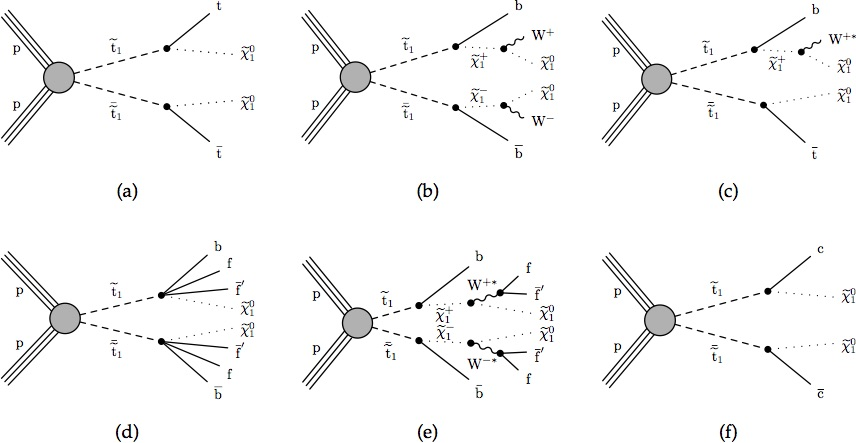
\includegraphics[width=1.00\textwidth]{T2tt_all.jpg}
	\end{center}
	\caption[Direct stop production]{Feynman diagrams for the direct \st{} production in SUSY. The allowed decay modes are (a) T2tt, (b) T2bW, (c) T2tb, (d,e) T2fbd, and (f) T2cc. }
	\label{fig:stop-direct-production}
\end{figure}

\begin{figure}[!h]
	\begin{center}
		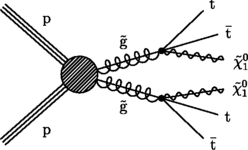
\includegraphics[width=0.32\textwidth]{T1tttt.png}
		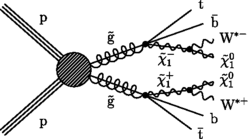
\includegraphics[width=0.32\textwidth]{T1ttbb.png} \\
		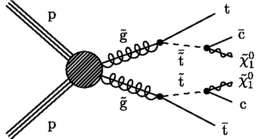
\includegraphics[width=0.32\textwidth]{T5ttcc.png}
		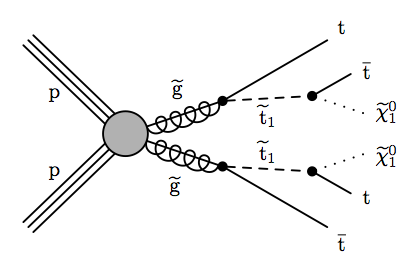
\includegraphics[width=0.32\textwidth]{T5tttt.png} \\
	\end{center}
	\caption[Gluino mediated stop production]{Feynman diagrams for the indirect \st{} production in SUSY. The allowed decay modes are T1tttt (top left), T1ttbb (top right), T5ttcc (bottom left), and T5tttt (bottom right).
	}
	\label{fig:stop-gluino-production}
\end{figure}


The main decay mode of the top squark is $\st\rightarrow t+\neutralino$ and $\st\rightarrow b+\chargino$, Fig. \ref{fig:stop-direct-production}. The top quark most likely decays as, $t\rightarrow b\W^+$, while the $b$ quark will decay to either a $c$ or an $u$ quark in its decay chain with an additional \W{} boson. The \neutralino{} is proposed to be a stable dark matter candidate while the \chargino{} could decay as, $\chargino\rightarrow\neutralino\W$. Next, a four body decay is allowed for, $\st\rightarrow b f f^\prime \neutralino$, see Fig. \ref{fig:stop-direct-production}(d, e). The final direct \st{} production we are interested in is the $\st\rightarrow c\neutralino$, see Fig. \ref{fig:stop-direct-production}(f). To be as inclusive as possible, we are also including indirect top squark production \cite{cms_collaboration_search_2013} as seen in Fig. \ref{fig:stop-gluino-production}. We see that the \st{} will decay to multiple jets, \nj, and missing transverse energy, \met. Now we are going to try to estimate the SM background that could be in each of our search region bins.

\section{Standard Model Background}
\label{sec:SMBackground}

The standard model background for the top squark search is defined by a large \met{} and multiple jets. The are a couple types of SM background that can be misinterpreted as our signal. The most likely background is that which causes many tops (or heavy particles) and missing energy. Events in the SM like \ttbar{} and \W+jets will have many jets produced and \met{} due to a missed lepton and neutrino. The production of heavy particles like \Znunu{} will give multiple jets and \met{} from the neutrinos being missed by the detector. QCD events often produce events with multiple jets. Due to acceptances in the detector jets can sometimes be mis-measured which can cause large \met{}. There are also various processes that are quite rare but still need to be included. We will take an in-depth look into each of these backgrounds. 

\section{Lost Lepton}
\label{sec:LL}

\begin{figure}
	\begin{center}
  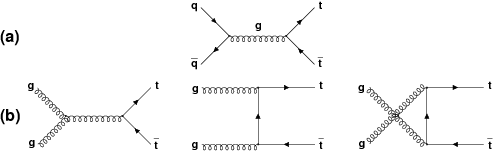
\includegraphics[width=0.9\textwidth]{LL/ttbar_diagrams.png}\\
  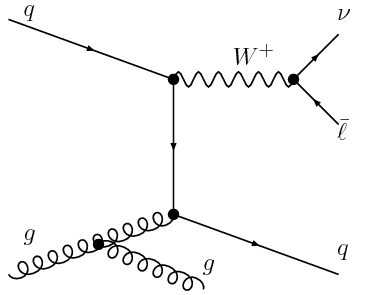
\includegraphics[width=0.30\textwidth]{LL/wjets_diagrams.png}
  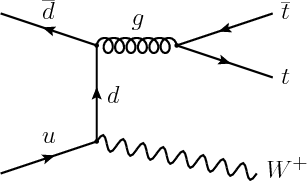
\includegraphics[width=0.30\textwidth]{LL/TTW_diagrams.png} 
  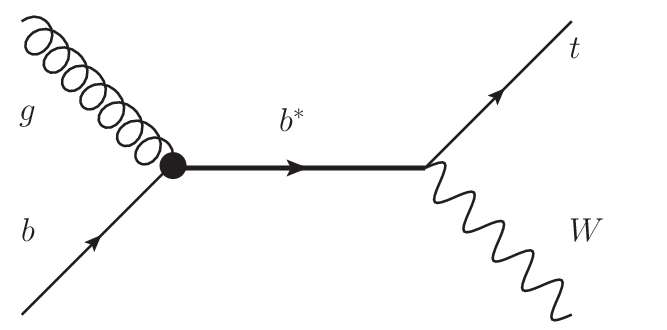
\includegraphics[width=0.30\textwidth]{LL/tW_diagrams.png} \\

	\caption[\ttbar{} Production]{Production Feynman diagrams for the LL backgrounds \cite{fiedler_precision_nodate, khachatryan_search_2016, aad_measurement_2013}. }
	\label{fig:llb-ttbar-diagram}
	\end{center}
\end{figure}

The contribution from the \ttbar{} and \W+jets processes arise from leptonic decays of the \W{} boson, where the charged lepton is outside the kinematic acceptance of CMS or evades identification by the dedicated lepton vetoes. Large \met{} can be generated by the associated neutrino and the lepton that is not reconstructed, allowing such events to enter the search regions. This background is collectively referred to as the "Lost Lepton" (LL) background. Contributions arising from $tW, ttW$ and single-top processes also enter into this category, but with much smaller importance. 

Studies of simulated events, indicate that the event kinematics for different lepton flavors are similar enough to allow us to estimate them collectively from a single control sample in data that has event characteristics similar to those of the search sample. Because of this, we use the single-lepton control sample to estimate the LL background, using the method described in detail in Ref. \cite{bravo_search_2015}. The single-lepton sample consists of events that have one lepton satisfying the lepton-veto criteria. In order to suppress potential signal contamination, we require $M_T(l,\met)<100~\GeV$. The requirement of low $M_T(l,\met)$ also ensures orthogonality to the search regions used in direct top squark production in the single-lepton or double-lepton final state, making it possible to statistically combine the results of the two searches. The selection applied to the single-lepton control sample follows the same selection on the search variables as in the zero-lepton selection with the exception of classification according to the number of top and \W-tagged candidates. 

\subsection{Combining All Run 2 Eras}\label{sec:LLCombination}
Firstly, each year of data can have a different detector configuration and corresponding simulation. These are split into separate eras that have accurate modeling of the data. We have defined five different eras for the data and simulation, 2016, 2017 RunBtoE, 2017 RunF, 2018 preHEM, and 2018 postHEM. The splits for 2017 are due to different average pileup and 2018 is split to take into account the loss of a part of the HCAL. For this analysis we are interested in the possibility of combining the yields of each era into one estimation. This is initially done by looking at the \met{} distributions in each era. Since the LL estimation is done with the transfer factor method, a good confirmation would be the comparison of the transfer factor in each SR for each era. 
\begin{figure}[!htb]
	\begin{center}
  \includegraphics[width=0.32\textwidth]{../Research/SUSY/2019/LLB/njets20_v3/MET_pt_DataMC___llcr_lm_RunBtoE_2017_allPU.pdf}
  \includegraphics[width=0.32\textwidth]{../Research/SUSY/2019/LLB/njets20_v3/MET_pt_DataMC___llcr_lm_RunF_2017_allPU.pdf} \\
  \includegraphics[width=0.32\textwidth]{../Research/SUSY/2019/LLB/njets20_v3/MET_pt_DataMC___llcr_lm_PreHEM_2018_allPU.pdf}
  \includegraphics[width=0.32\textwidth]{../Research/SUSY/2019/LLB/njets20_v3/MET_pt_DataMC___llcr_lm_PostHEM_2018_allPU.pdf} \\
	\end{center}
	\caption{Comparison of the Data and MC in the 1Lep CR for each era: Run2016, Run2017BtoE, Run2017F, Run2018preHEM, Run2018PostHEM, and the combination of all eras in the Low \dm{} region. Each era has a good agreement between Data and MC. 
	 }
	\label{fig:llb-1lcr-datavsmc-lm-inclusive}
\end{figure}
\begin{figure}[!htb]
	\begin{center}  
		\includegraphics[width=0.32\textwidth]{../Research/SUSY/2019/LLB/njets20_v3/MET_pt_DataMC___llcr_hm_RunBtoE_2017_allPU.pdf}
		\includegraphics[width=0.32\textwidth]{../Research/SUSY/2019/LLB/njets20_v3/MET_pt_DataMC___llcr_hm_RunF_2017_allPU.pdf} \\
		\includegraphics[width=0.32\textwidth]{../Research/SUSY/2019/LLB/njets20_v3/MET_pt_DataMC___llcr_hm_PreHEM_2018_allPU.pdf}
		\includegraphics[width=0.32\textwidth]{../Research/SUSY/2019/LLB/njets20_v3/MET_pt_DataMC___llcr_hm_PostHEM_2018_allPU.pdf}
	\end{center}
	\caption{Comparison of the Data and MC in the 1Lep CR for each era: Run2016, Run2017BtoE, Run2017F, Run2018preHEM, Run2018PostHEM, and the combination of all eras in the High \dm{} region. Each era has a good agreement between Data and MC. 
	 }
	\label{fig:llb-1lcr-datavsmc-hm-inclusive}
\end{figure}


\subsection{Transfer Factors}
\label{subsec:TF}

The LL estimation in each search region is based upon the event count in data in the corresponding control region in the single-lepton sample. The count is extrapolated to the search region to obtain a prediction by means of a transfer factor obtained from simulation as follows: 

\begin{equation}
\label{eqn:LLTF}
N_{pred}^{LL}=TF_{LL} \cdot N_{data}(1l).
\end{equation}

This allows us to have the same selection for the single-lepton control sample and the zero-lepton sample. The only exception is the number of top and W-tagged candidates. The LL estimation is dependent on the yield of data in the corresponding CR and the TF calculated by the single-lepton sample. The transfer factor is defined as, 
\begin{equation}
\label{eqn:TF}
TF_{LL}=\frac{N_{MC}(0l)}{N_{MC}(1l)},
\end{equation}
where $N_{MC}(1l)$ is the event count observed in the corresponding CR and $N_{MC}(0l)$ uses the event count in the corresponding SR. 

The main motivation behind this approach is to increase the statistical precision of the background estimation. The performance of the $t$ and \W{} taggers has been studied in data and MC samples and a reasonably good agreement is observed allowing us to proceed with this approach. Data-to-MC scale factors are extracted and applied to MC to account for residual differences of the tagging performance in data. Detailed studies comparing the performance of the $t$ and \W{} taggers in data and MC are found in Ref. \cite{cms_collaboration_search_2016}.

The control regions utilized to predict the LL background are displayed in Figs. \ref{fig:llb-1lcr-datavsmc-lm-nb0} to \ref{fig:llb-1lcr-datavsmc-hm-nb3-1}. Figures \ref{fig:llb-1lcr-datavsmc-lm-nb0} and \ref{fig:llb-1lcr-datavsmc-lm-nb1} display the control regions specific to the low \dm{} selection, where the regions are binned following the search region definition. Figures \ref{fig:llb-1lcr-datavsmc-hm-nt0-nrt0-nw0} to \ref{fig:llb-1lcr-datavsmc-hm-nb3-1} display the control regions dedicated for the high \dm{} selection. Due to the nature of the background estimation method applied in the high \dm{} search, control regions are utilized for the prediction of multiple search regions. 

Tables \ref{tab:0l-llb-pred-lm} to \ref{tab:0l-llb-pred-hm-3} summarize the yields in data observed in the single-lepton sample, the derived transfer factor, and the resulting LL predictions for the low \dm{} and high \dm{} search regions, respectively. The transfer factors in the high \dm{} region actually account for two levels of extrapolation. The CR for the high \dm{} is loose, such that, there is no binning in tops or W tagging. We then extrapolate to the SR with the inclusion of the top and W tags, along with scale factors, to estimate the LL background in the region with:
\begin{equation}\label{TFExtrapolation}
\begin{split}
\tfll=& \tfll^{CR-SR}\times \tfll^{SR-extrap} \\
=& \frac{N_{MC}(0l)(\nj,\nb,\met)}{N_{MC}(1l)(\nj,\nb,\met)}\times\frac{N_{MC}(0l)(\nj,\nb,\met,\nt,\nrt,\nw)}{N_{MC}(0l)(\nj,\nb,\met)}.
\end{split}
\end{equation}

We now want to consider how the transfer factor for each era relates to the total transfer factor. In Figs. \ref{fig:llb-1lcr-datavsmc-total-tf} and \ref{fig:llb-1lcr-datavsmc-sep-tf}, we see the comparison for the total \tfll{} for each era of the data and simulation. These are all in quite good agreement, but we see an extended tail due to the low statistics of the extrapolation in $t$ and \W. Once we alter the comparison for the \tfll{} to separate the CR-to-SR and the SR-to-Extrapolation, we see a much better agreement when for the CR-to-SR comparison. These are improved because of the better statistics in the region. 
\begin{figure}
	\begin{center}
  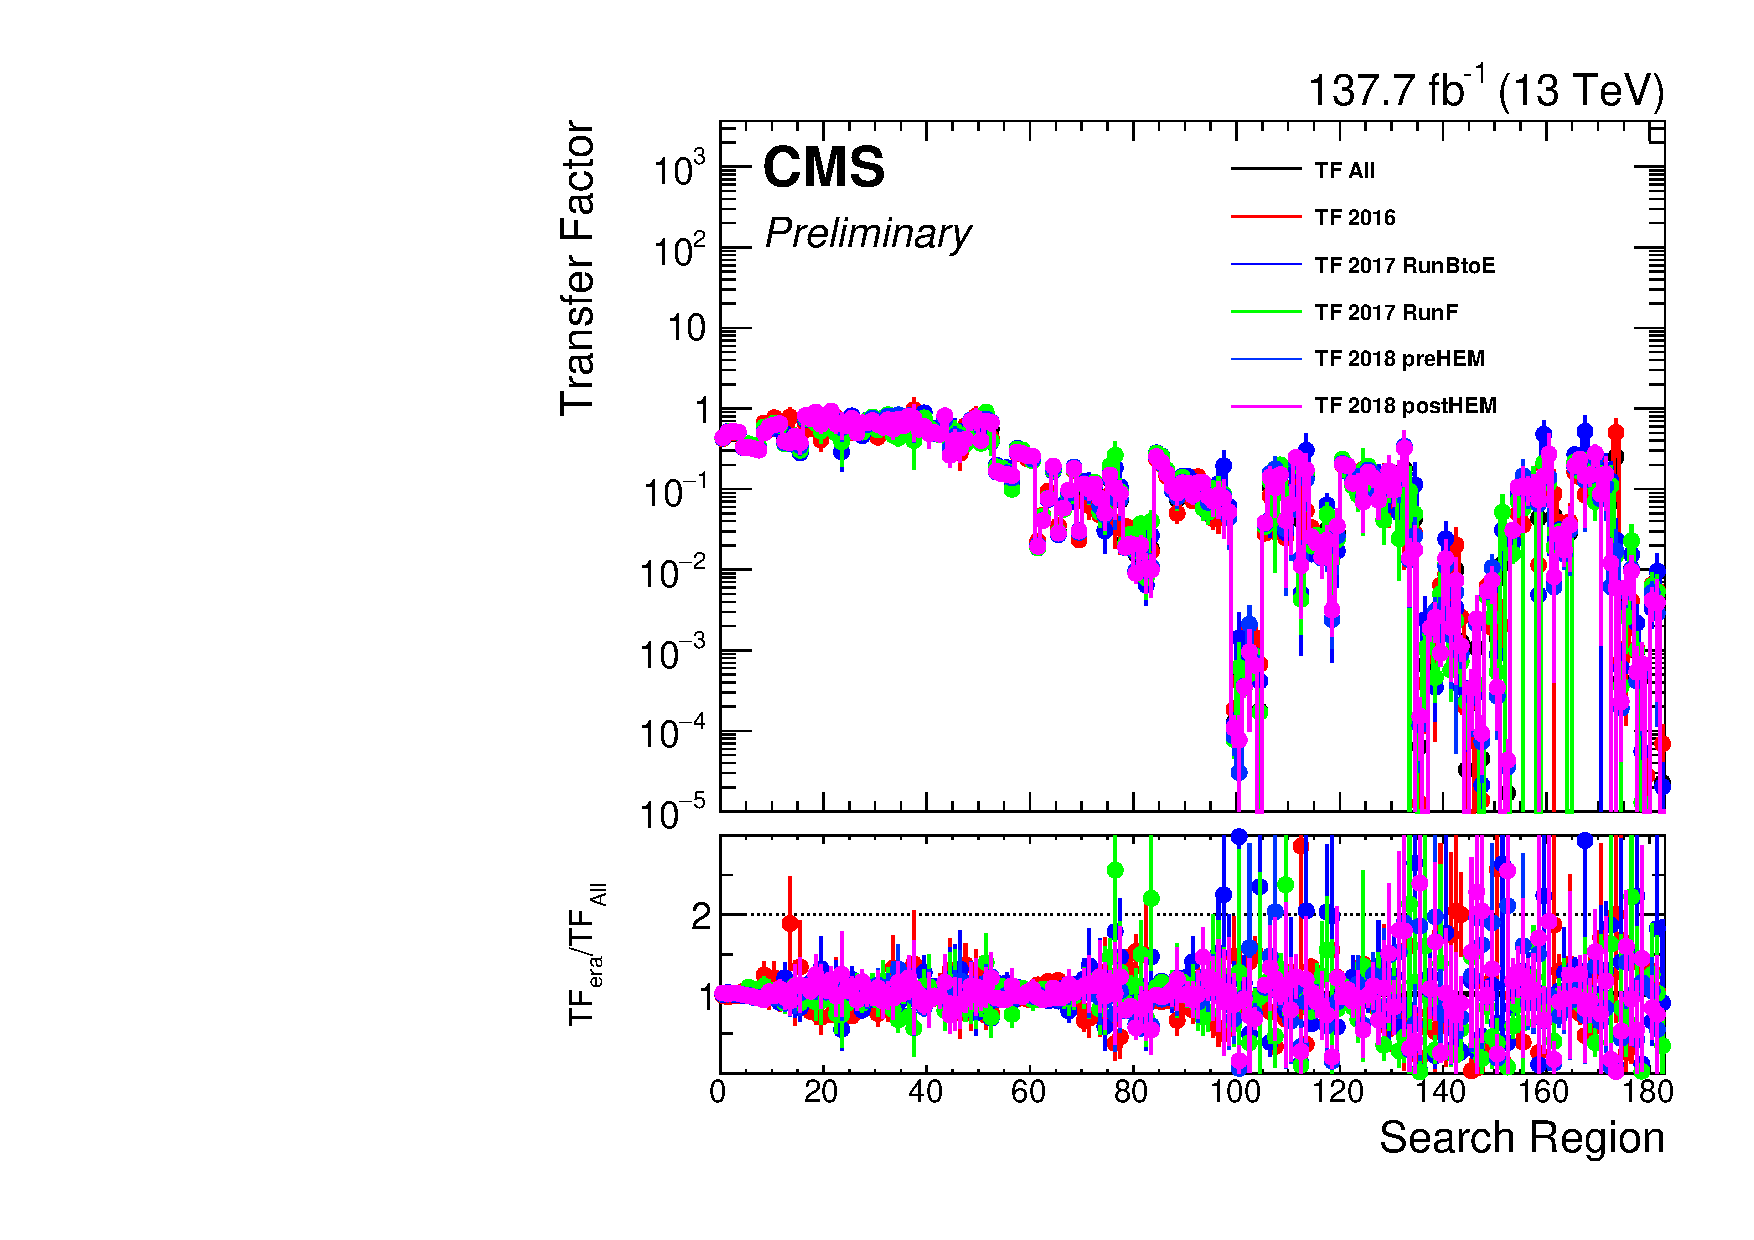
\includegraphics[width=0.4\textwidth]{LostLepton_TF_Comparison.pdf}
  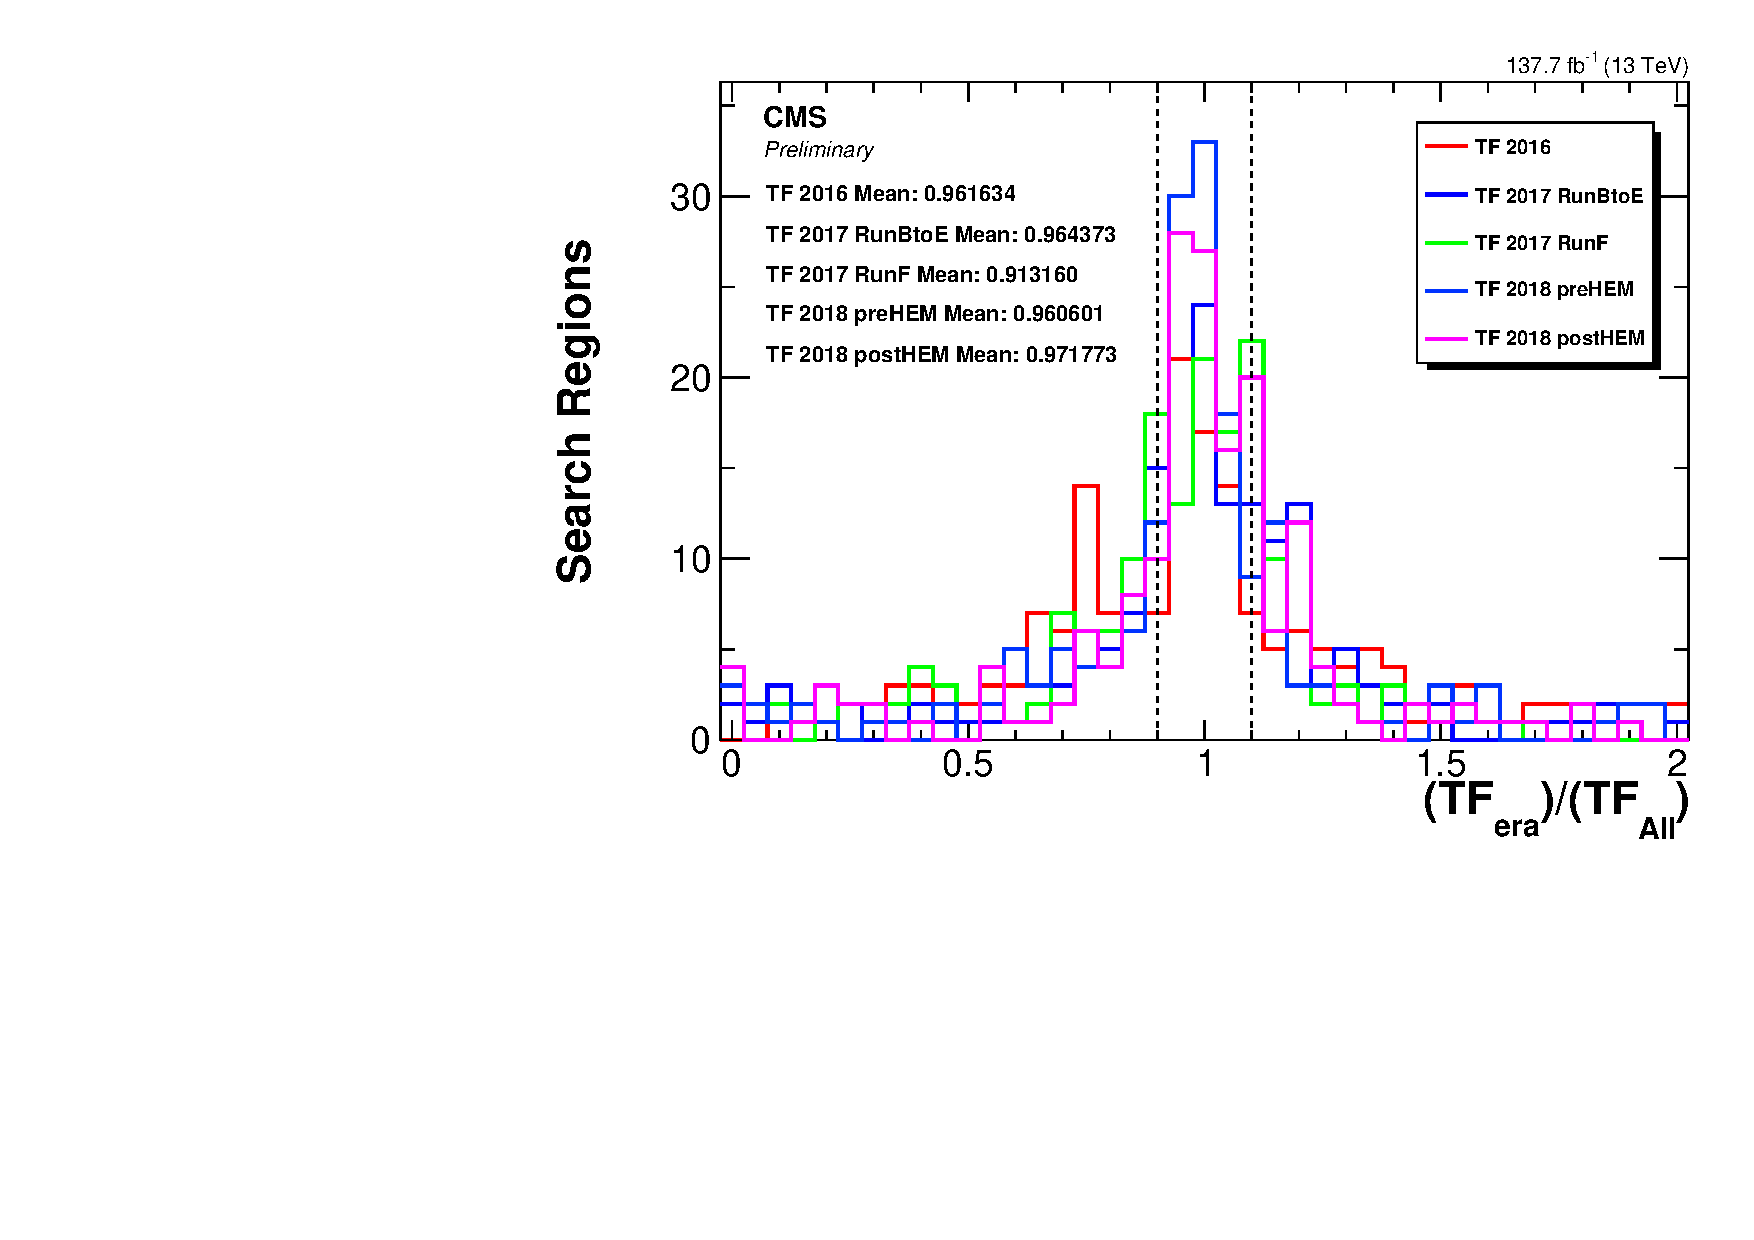
\includegraphics[width=0.5\textwidth]{LostLepton_TF_Comparison_sum.pdf} \\
	\end{center}
	\caption[Transfer Factor Comparison]{Comparisons of the transfer factors for each era of MC in the low and high \dm{} regions. The values are shown in their separate bins on the left plot and in a combined form on the right. The mean for each is also shown. 
	 }
	\label{fig:llb-1lcr-datavsmc-total-tf}
\end{figure}
\begin{figure}
	\begin{center}  
		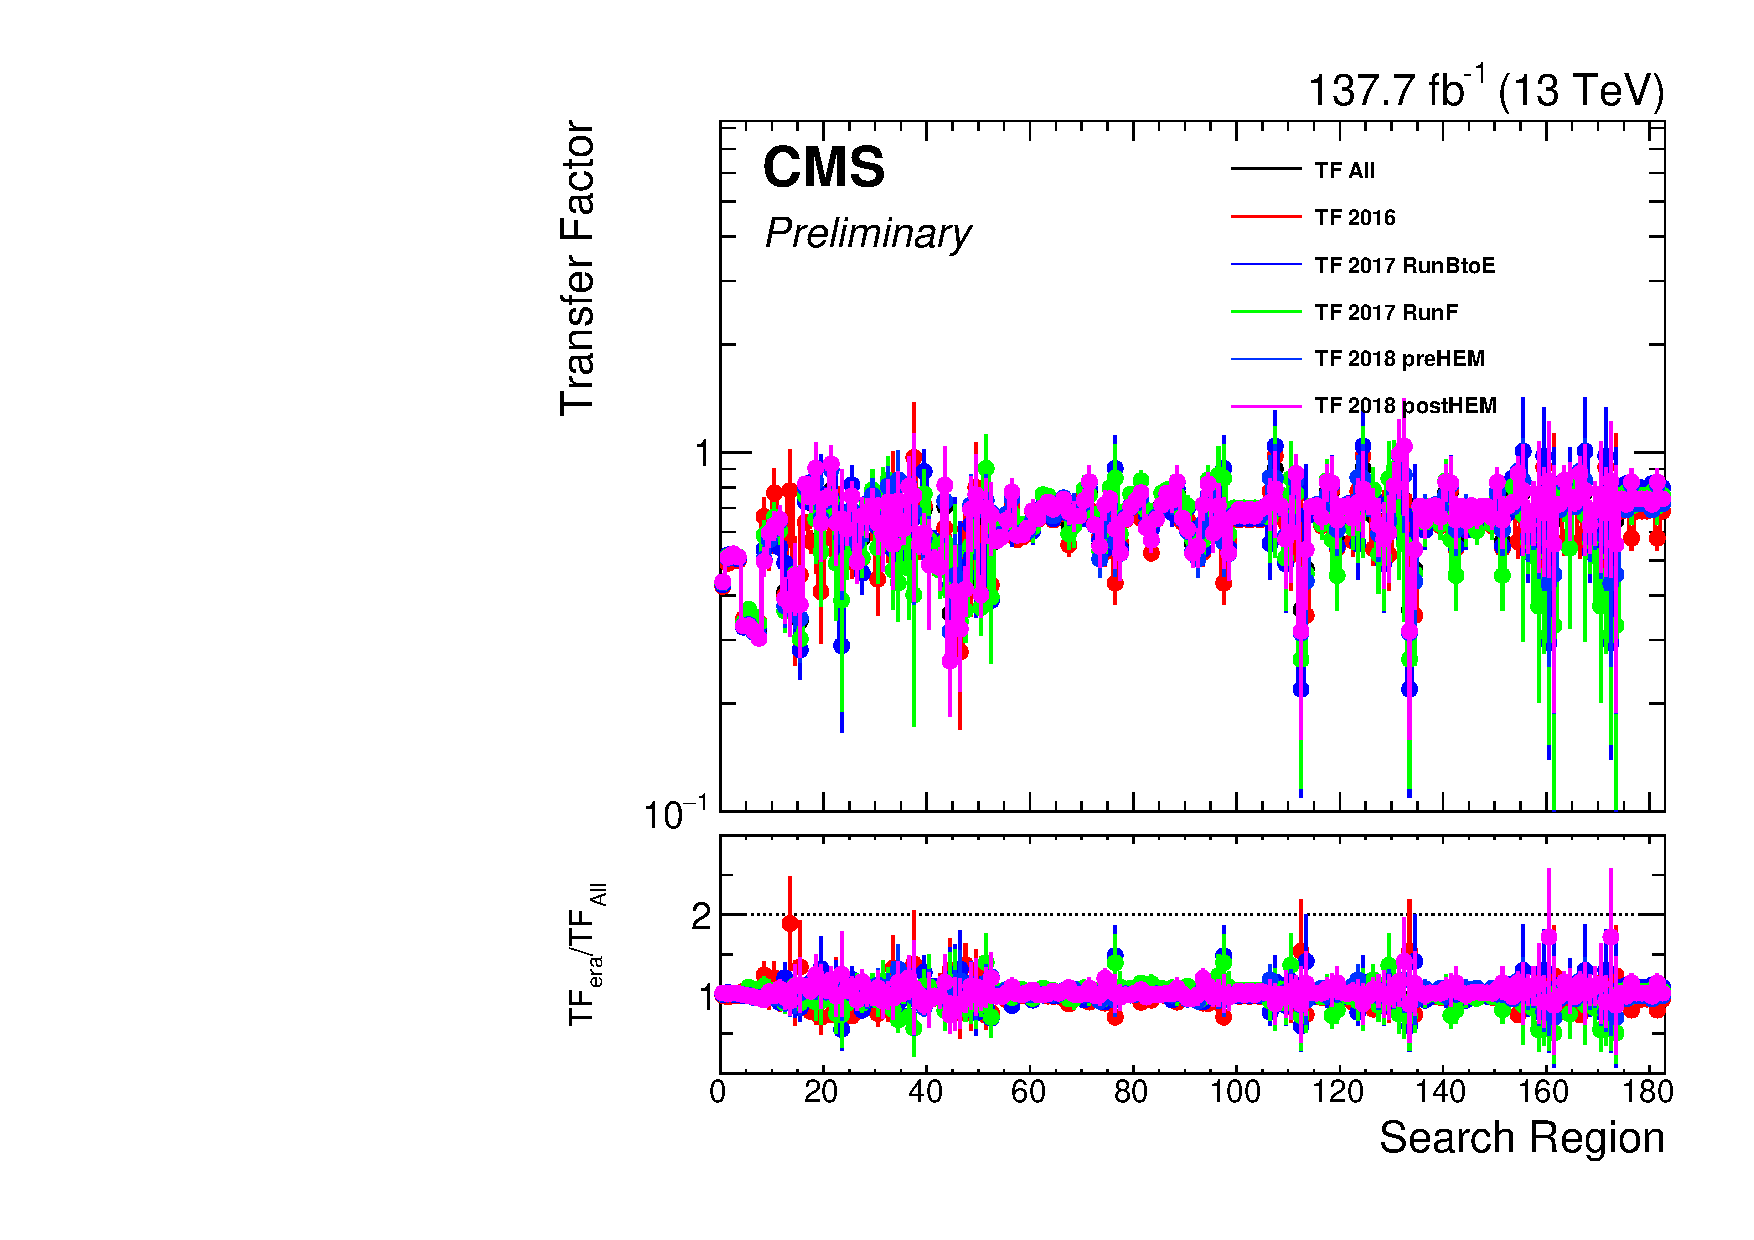
\includegraphics[width=0.4\textwidth]{LostLepton_TF_CR_to_SR_noextrap_Comparison.pdf}
		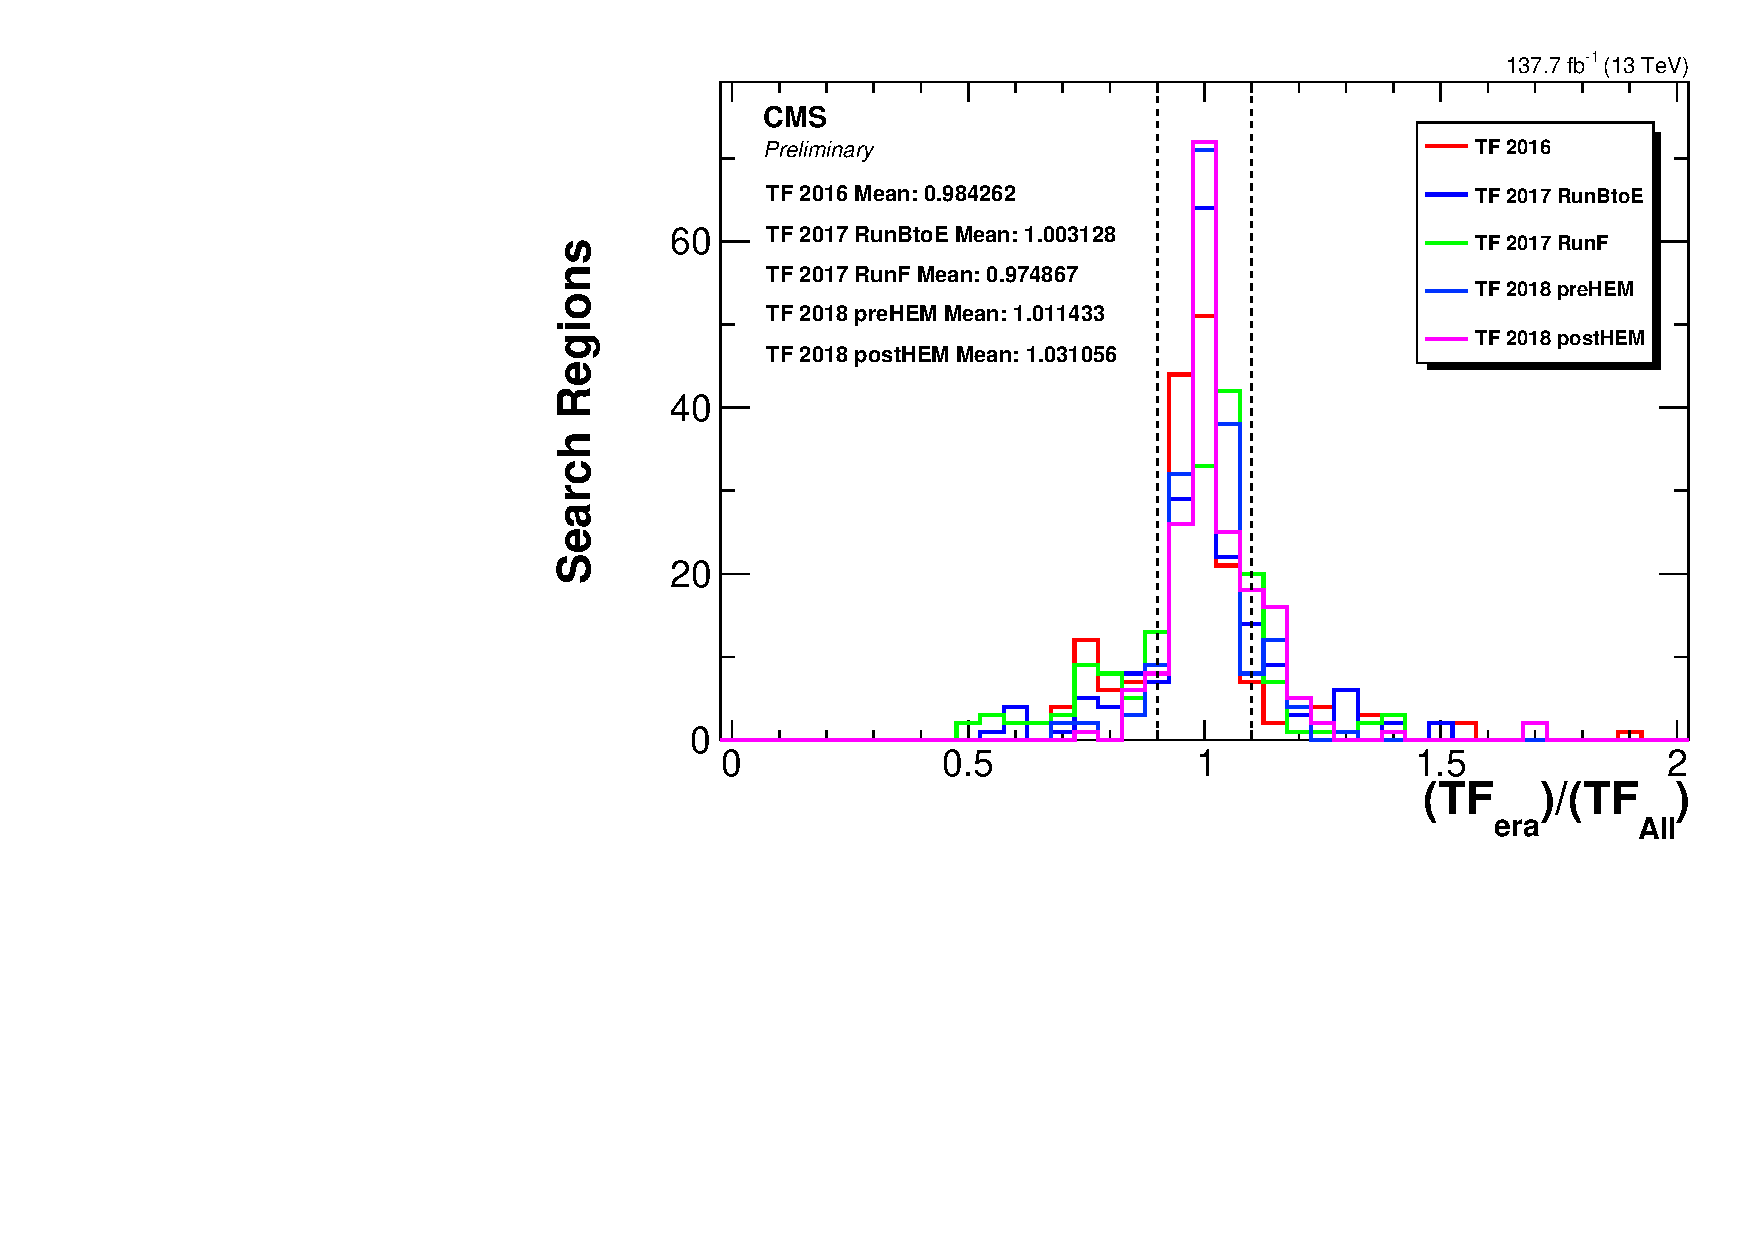
\includegraphics[width=0.5\textwidth]{LostLepton_TF_CR_to_SR_noextrap_Comparison_sum.pdf} \\
		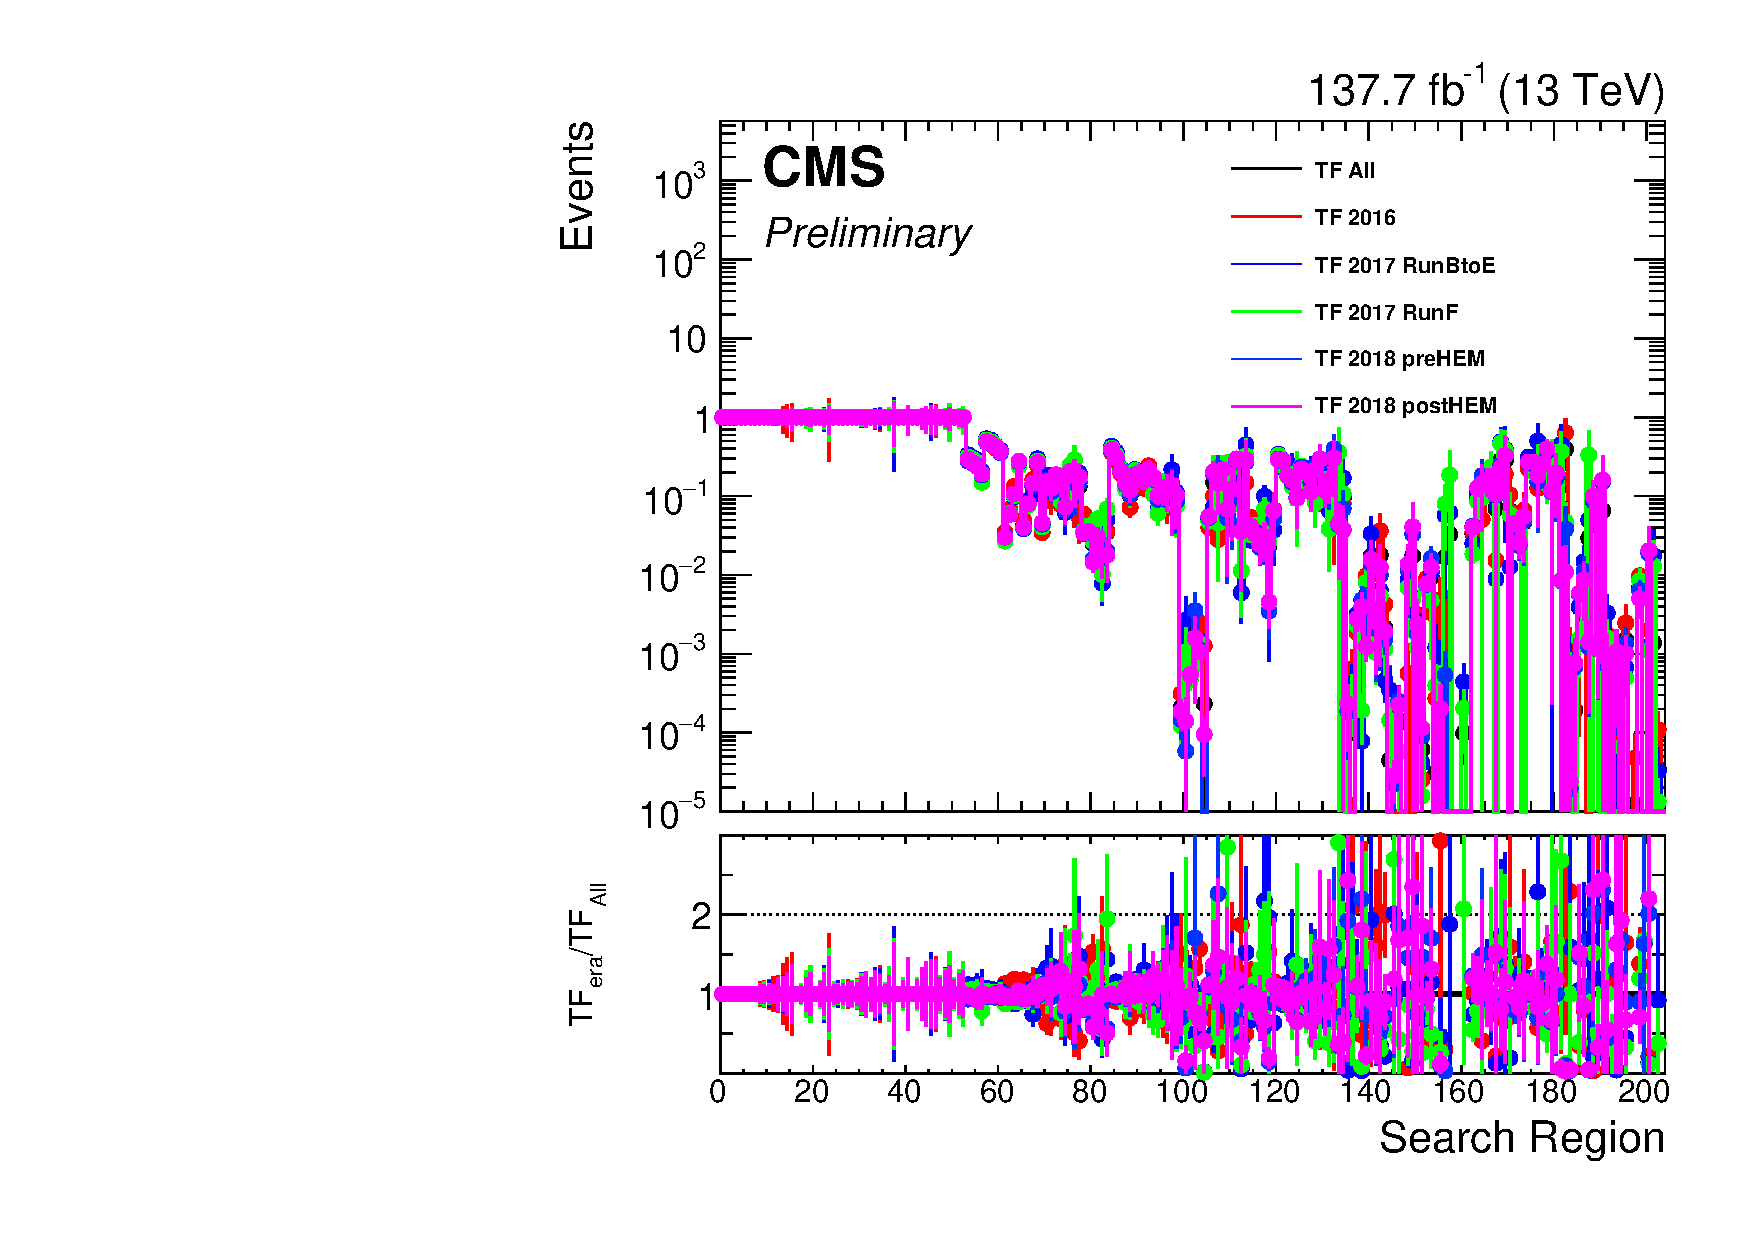
\includegraphics[width=0.4\textwidth]{LostLepton_TF_SR_extrap_Comparison.pdf}
		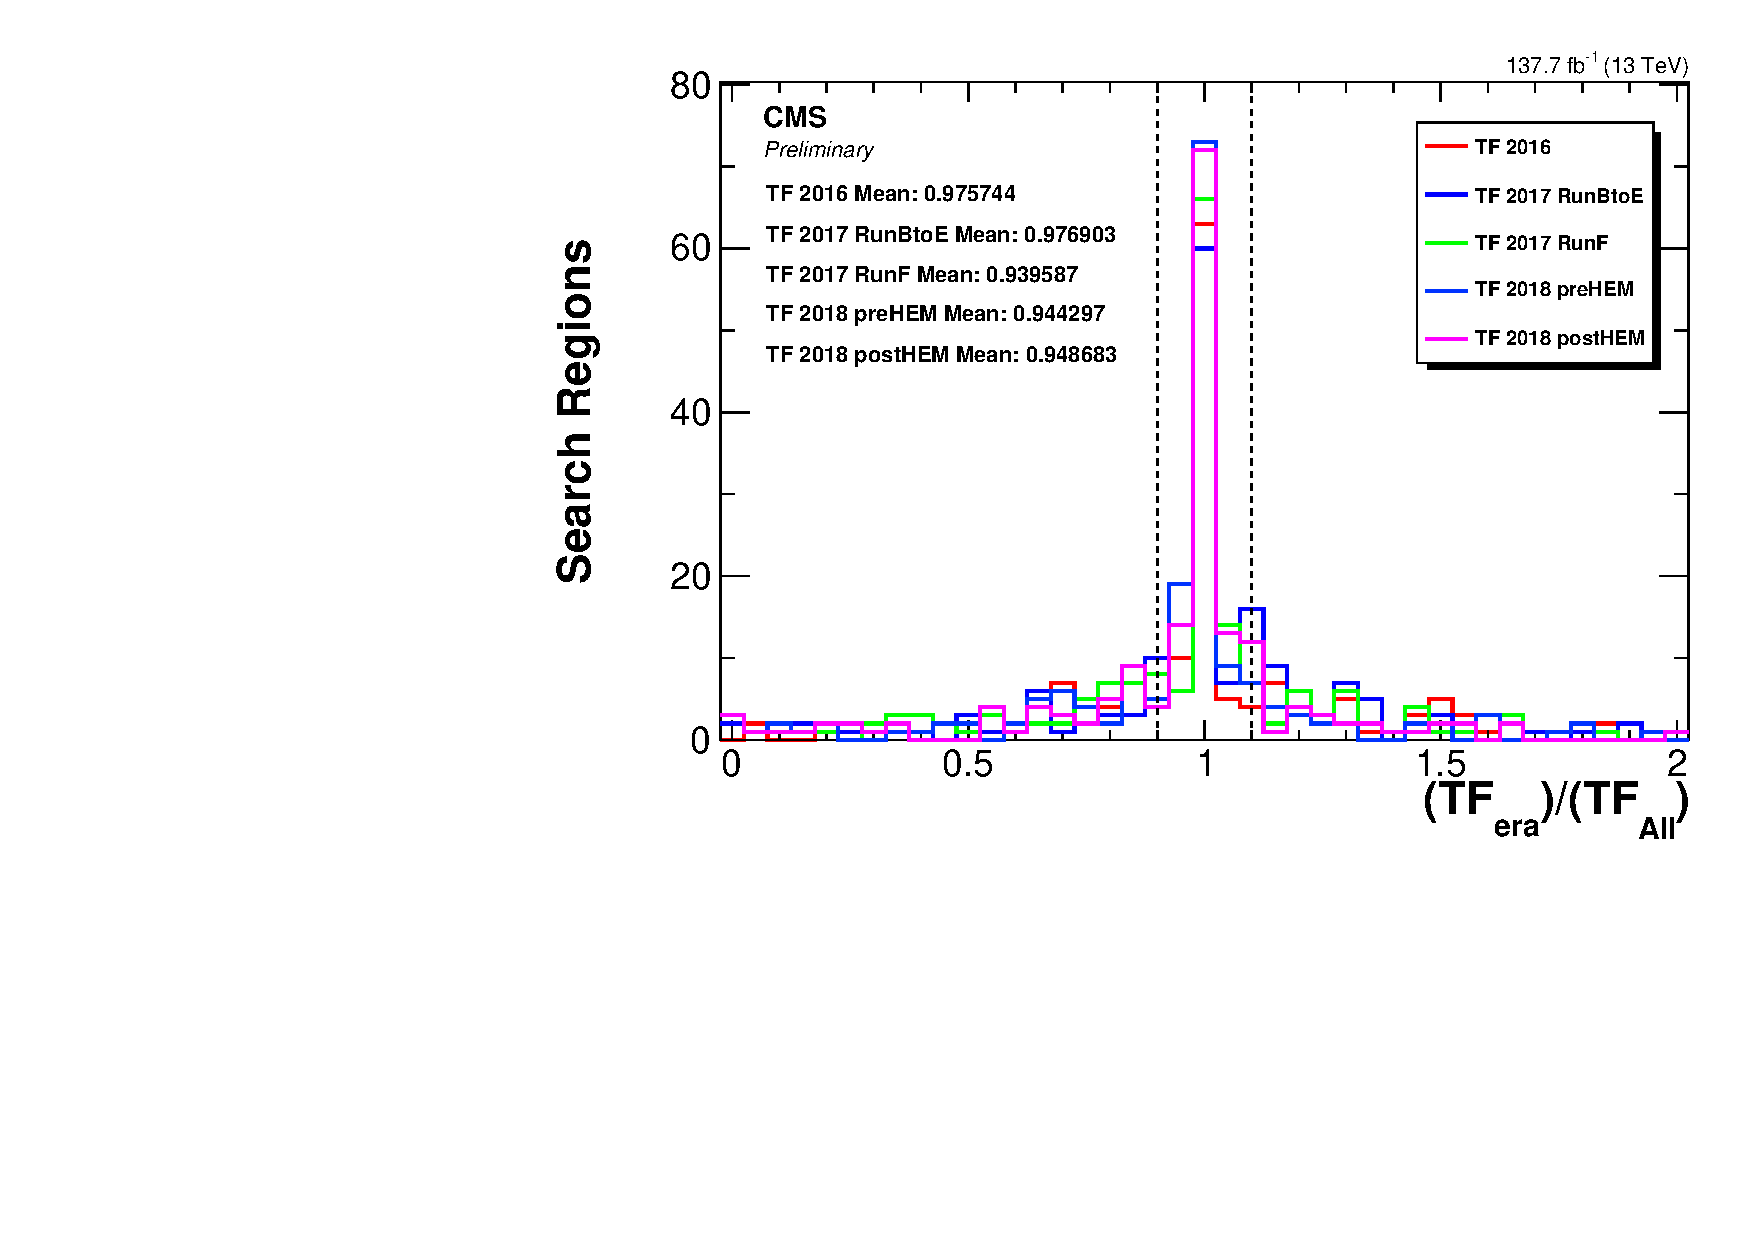
\includegraphics[width=0.5\textwidth]{LostLepton_TF_SR_extrap_Comparison_sum.pdf}
	\end{center}
	\caption[Separated Transfer Factor Comparison]{Comparisons of the transfer factors, separated into the CR-to-SR (top) and SR-to-extrapolation (bottom), for each era of MC in the low and high \dm{} regions. The values are shown in their separate bins on the left plot and in a combined form on the right. The mean for each is also shown. 
	 }
	\label{fig:llb-1lcr-datavsmc-sep-tf}
\end{figure}

% matches pred table
% copy and paste the output from the end of LLBPred() (it calls printMoriond17Table) between the below labels "start insert" and "stop insert".
\begin{table}[!!htbp]
\begin{center}
\resizebox*{0.6\textwidth}{!}{
\begin{tabular}{|c||c||c|c|c|}
\hline
Search Region & \met [GeV] & $N_{\text{data}}(1l)$ & $\tfll$ & $N_\text{pred}^{\text{LL}}$ \\
\hline
% Search region & 	$\met$ & 	singlelep & 	_TF & 	_pred & 	
\hline
\multicolumn{5}{c}{low \dm, $\nb=0$, $\nsv=0$, $\ptisr\geq500$\,GeV, $2\leq\nj\leq5$} \\
\hline
 %  lm_nb0_nivf0_highptisr_nj2to5
0 & 450$-$550 & 	5045 & 	0.432$\pm$0.004 & 	2178.23$\pm$35.68 \\
1 & 550$-$650 & 	2198 & 	0.509$\pm$0.004 & 	1118.77$\pm$25.67 \\
2 & 650$-$750 & 	818 & 	0.516$\pm$0.004 & 	421.97$\pm$15.16 \\
3 & $\geq750$ & 	540 & 	0.509$\pm$0.004 & 	274.59$\pm$12.04 \\
\hline
\multicolumn{5}{c}{low \dm, $\nb=0$, $\nsv=0$, $\ptisr\geq500$\,GeV, $\nj\geq6$} \\
\hline
 %     lm_nb0_nivf0_highptisr_nj6
4 & 450$-$550 & 	849 & 	0.333$\pm$0.004 & 	282.81$\pm$10.32 \\
5 & 550$-$650 & 	408 & 	0.338$\pm$0.005 & 	137.77$\pm$7.14 \\
6 & 650$-$750 & 	181 & 	0.331$\pm$0.006 & 	59.90$\pm$4.60 \\
7 & $\geq750$ & 	156 & 	0.321$\pm$0.006 & 	50.12$\pm$4.11 \\
\hline
\multicolumn{5}{c}{low \dm, $\nb=0$, $\nsv\geq1$, $\ptisr\geq500$\,GeV, $2\leq\nj\leq5$} \\
\hline
 %  lm_nb0_nivf1_highptisr_nj2to5
8 & 450$-$550 & 	148 & 	0.537$\pm$0.024 & 	79.42$\pm$7.44 \\
9 & 550$-$650 & 	38 & 	0.581$\pm$0.026 & 	22.09$\pm$3.71 \\
10 & 650$-$750 & 	25 & 	0.641$\pm$0.032 & 	16.03$\pm$3.31 \\
11 & $\geq750$ & 	16 & 	0.609$\pm$0.027 & 	9.75$\pm$2.48 \\
\hline
\multicolumn{5}{c}{low \dm, $\nb=0$, $\nsv\geq1$, $\ptisr\geq500$\,GeV, $\nj\geq6$} \\
\hline
 %     lm_nb0_nivf1_highptisr_nj6
12 & 450$-$550 & 	43 & 	0.410$\pm$0.028 & 	17.64$\pm$2.96 \\
13 & 550$-$650 & 	12 & 	0.415$\pm$0.037 & 	4.98$\pm$1.50 \\
14 & 650$-$750 & 	5 & 	0.414$\pm$0.040 & 	2.07$\pm$0.95 \\
15 & $\geq750$ & 	4 & 	0.341$\pm$0.041 & 	1.36$\pm$0.70 \\
\hline
\multicolumn{5}{c}{low \dm, $\nb=1$, $\nsv=0$, $\mtb<175$~\GeV, $300\leq\ptisr<500$\,GeV, $\ptb<40$\,GeV} \\
\hline
 % lm_nb1_nivf0_lowmtb_lowptisr_lowptb
16 & 300$-$400 & 	2037 & 	0.746$\pm$0.015 & 	1520.34$\pm$45.84 \\
17 & 400$-$500 & 	341 & 	0.724$\pm$0.031 & 	246.78$\pm$16.96 \\
18 & 500$-$600 & 	32 & 	0.726$\pm$0.061 & 	23.24$\pm$4.55 \\
19 & $\geq600$ & 	6 & 	0.581$\pm$0.068 & 	3.48$\pm$1.48 \\
\hline
\multicolumn{5}{c}{low \dm, $\nb=1$, $\nsv=0$, $\mtb<175$~\GeV, $300\leq\ptisr<500$\,GeV, $40<\ptb<70$\,GeV} \\
\hline
 % lm_nb1_nivf0_lowmtb_lowptisr_medptb
20 & 300$-$400 & 	1015 & 	0.716$\pm$0.019 & 	726.30$\pm$29.71 \\
21 & 400$-$500 & 	127 & 	0.786$\pm$0.047 & 	99.84$\pm$10.68 \\
22 & 500$-$600 & 	11 & 	0.655$\pm$0.076 & 	7.21$\pm$2.33 \\
23 & $\geq600$ & 	6 & 	0.524$\pm$0.115 & 	3.15$\pm$1.46 \\
\hline
\multicolumn{5}{c}{low \dm, $\nb=1$, $\nsv=0$, $\mtb<175$~\GeV, $\ptisr\geq500$\,GeV, $\ptb<40$\,GeV} \\
\hline
 % lm_nb1_nivf0_lowmtb_highptisr_lowptb
24 & 450$-$550 & 	136 & 	0.579$\pm$0.027 & 	78.76$\pm$7.72 \\
25 & 550$-$650 & 	45 & 	0.686$\pm$0.034 & 	30.87$\pm$4.85 \\
26 & 650$-$750 & 	12 & 	0.537$\pm$0.033 & 	6.44$\pm$1.90 \\
27 & $\geq750$ & 	14 & 	0.576$\pm$0.034 & 	8.07$\pm$2.21 \\
\hline
\multicolumn{5}{c}{low \dm, $\nb=1$, $\nsv=0$, $\mtb<175$~\GeV, $\ptisr\geq500$\,GeV, $40<\ptb<70$\,GeV} \\
\hline
 % lm_nb1_nivf0_lowmtb_highptisr_medptb
28 & 450$-$550 & 	89 & 	0.676$\pm$0.039 & 	60.14$\pm$7.25 \\
29 & 550$-$650 & 	19 & 	0.722$\pm$0.045 & 	13.72$\pm$3.26 \\
30 & 650$-$750 & 	11 & 	0.589$\pm$0.053 & 	6.47$\pm$2.04 \\
31 & $\geq750$ & 	3 & 	0.654$\pm$0.066 & 	1.96$\pm$1.15 \\
\hline
\multicolumn{5}{c}{low \dm, $\nb=1$, $\nsv\geq1$, $\mtb<175$~\GeV, $\ptb<40$\,GeV} \\
\hline
 %     lm_nb1_nivf1_lowmtb_lowptb
32 & 300$-$400 & 	115 & 	0.741$\pm$0.054 & 	85.23$\pm$10.10 \\
33 & 400$-$500 & 	26 & 	0.587$\pm$0.069 & 	15.26$\pm$3.49 \\
34 & $\geq500$ & 	13 & 	0.640$\pm$0.071 & 	8.32$\pm$2.49 \\
\hline
\multicolumn{5}{c}{low \dm, $\nb\geq2$, $\mtb<175$~\GeV, $300\leq\ptisr<500$\,GeV, $\ptbonetwo<80$\,GeV} \\
\hline
 % lm_nb2_lowmtb_lowptisr_lowptb12
35 & 300$-$400 & 	242 & 	0.603$\pm$0.028 & 	145.92$\pm$11.59 \\
36 & 400$-$500 & 	36 & 	0.667$\pm$0.066 & 	24.00$\pm$4.65 \\
37 & $\geq500$ & 	7 & 	0.704$\pm$0.169 & 	4.93$\pm$2.21 \\
\hline
\multicolumn{5}{c}{low \dm, $\nb\geq2$, $\mtb<175$~\GeV, $300\leq\ptisr<500$\,GeV, $80<\ptbonetwo<140$\,GeV} \\
\hline
 % lm_nb2_lowmtb_lowptisr_medptb12
38 & 300$-$400 & 	579 & 	0.554$\pm$0.015 & 	320.86$\pm$15.79 \\
39 & 400$-$500 & 	101 & 	0.694$\pm$0.045 & 	70.12$\pm$8.31 \\
40 & $\geq500$ & 	16 & 	0.525$\pm$0.081 & 	8.40$\pm$2.47 \\
\hline
\multicolumn{5}{c}{low \dm, $\nb\geq2$, $\mtb<175$~\GeV, $300\leq\ptisr<500$\,GeV, $\ptbonetwo\geq140$\,GeV, $\nj\geq7$} \\
\hline
 % lm_nb2_lowmtb_lowptisr_highptb12_nj7
41 & 300$-$400 & 	318 & 	0.516$\pm$0.016 & 	164.19$\pm$10.49 \\
42 & 400$-$500 & 	53 & 	0.494$\pm$0.031 & 	26.19$\pm$3.96 \\
43 & $\geq500$ & 	9 & 	0.706$\pm$0.088 & 	6.36$\pm$2.26 \\
\hline
\multicolumn{5}{c}{low \dm, $\nb\geq2$, $\mtb<175$~\GeV, $\ptisr\geq500$\,GeV, $\ptbonetwo<80$\,GeV} \\
\hline
 % lm_nb2_lowmtb_highptisr_lowptb12
44 & 450$-$550 & 	19 & 	0.356$\pm$0.047 & 	6.77$\pm$1.79 \\
45 & 550$-$650 & 	7 & 	0.469$\pm$0.075 & 	3.29$\pm$1.35 \\
46 & $\geq650$ & 	2 & 	0.366$\pm$0.057 & 	0.73$\pm$0.53 \\
\hline
\multicolumn{5}{c}{low \dm, $\nb\geq2$, $\mtb<175$~\GeV, $\ptisr\geq500$\,GeV, $80<\ptbonetwo<140$\,GeV} \\
\hline
 % lm_nb2_lowmtb_highptisr_medptb12
47 & 450$-$550 & 	50 & 	0.447$\pm$0.035 & 	22.33$\pm$3.60 \\
48 & 550$-$650 & 	16 & 	0.631$\pm$0.074 & 	10.10$\pm$2.79 \\
49 & $\geq650$ & 	6 & 	0.699$\pm$0.103 & 	4.20$\pm$1.82 \\
\hline
\multicolumn{5}{c}{low \dm, $\nb\geq2$, $\mtb<175$~\GeV, $\ptisr\geq500$\,GeV, $\ptbonetwo\geq140$\,GeV, $\nj\geq7$} \\
\hline
 % lm_nb2_lowmtb_highptisr_highptb12_nj7
50 & 450$-$550 & 	59 & 	0.429$\pm$0.027 & 	25.31$\pm$3.67 \\
51 & 550$-$650 & 	19 & 	0.649$\pm$0.063 & 	12.32$\pm$3.07 \\
52 & $\geq650$ & 	7 & 	0.559$\pm$0.070 & 	3.91$\pm$1.56 \\
\hline
\end{tabular}
}
\caption{\label{tab:0l-llb-pred-lm}The LL estimate in the various low \dm{} search regions, bins 0 to 53, using the \datalumi~dataset.}
\end{center}
\end{table}
% matches pred table
% copy and paste the output from the end of LLBPred() (it calls printMoriond17Table) between the below labels "start insert" and "stop insert".
\begin{table}[!h]
\begin{center}
\resizebox*{0.6\textwidth}{!}{
\begin{tabular}{|c||c||c|c|c|c|c|}
\hline
Search Region & \met [GeV] & $N_{\text{data}}(1l)$ & $\tfll$ & $\tfll^{\text{CR-SR}}$ & $\tfll^{\text{SR-extrap}}$ & $N_\text{pred}^{\text{LL}}$ \\
\hline
% Search region & 	$\met$ & 	singlelep & 	_TF & 	_TF_CR_to_SR_noextrap & 	_TF_SR_extrap & 	_pred & 	
\hline
\multicolumn{7}{c}{high \dm, $\nb=1$, $\mtb<175$~\GeV, $\nj\geq7$, $\nrt\geq1$} \\
\hline
 %      hm_nb1_lowmtb_nj7_nrtgeq1
53 & 250$-$300 & 	1151 & 	0.196$\pm$0.004 & 	0.519 & 	0.378 & 	225.43$\pm$8.24 \\
54 & 300$-$400 & 	697 & 	0.187$\pm$0.005 & 	0.550 & 	0.340 & 	130.35$\pm$6.21 \\
55 & 400$-$500 & 	129 & 	0.180$\pm$0.011 & 	0.577 & 	0.313 & 	23.26$\pm$2.53 \\
56 & $\geq500$ & 	43 & 	0.157$\pm$0.016 & 	0.598 & 	0.263 & 	6.77$\pm$1.25 \\
\hline
\multicolumn{7}{c}{high \dm, $\nb\geq2$, $\mtb<175$~\GeV, $\nj\geq7$, $\nrt\geq1$} \\
\hline
 %      hm_nb2_lowmtb_nj7_nrtgeq1
57 & 250$-$300 & 	2250 & 	0.292$\pm$0.004 & 	0.539 & 	0.542 & 	657.73$\pm$16.12 \\
58 & 300$-$400 & 	1256 & 	0.286$\pm$0.005 & 	0.548 & 	0.522 & 	359.11$\pm$11.69 \\
59 & 400$-$500 & 	236 & 	0.278$\pm$0.010 & 	0.582 & 	0.478 & 	65.56$\pm$4.92 \\
60 & $\geq500$ & 	99 & 	0.259$\pm$0.017 & 	0.625 & 	0.415 & 	25.67$\pm$3.06 \\
\hline
\multicolumn{7}{c}{high \dm, $\nb=1$, $\mtb\geq175$~\GeV, $\nt=0$, $\nrt=0$, $\nw=0$, $\Ht\geq1000$} \\
\hline
 % hm_nb1_highmtb_nt0_nrt0_nw0_htgt1000
61 & 250$-$350 & 	570 & 	0.383$\pm$0.007 & 	0.657 & 	0.583 & 	218.28$\pm$10.01 \\
62 & 350$-$450 & 	233 & 	0.369$\pm$0.011 & 	0.614 & 	0.602 & 	86.03$\pm$6.16 \\
63 & 450$-$550 & 	102 & 	0.362$\pm$0.015 & 	0.544 & 	0.666 & 	36.97$\pm$3.96 \\
64 & $\geq550$ & 	109 & 	0.352$\pm$0.013 & 	0.531 & 	0.663 & 	38.39$\pm$3.93 \\
\hline
\multicolumn{7}{c}{high \dm, $\nb\geq2$, $\mtb\geq175$~\GeV, $\nt=0$, $\nrt=0$, $\nw=0$, $\Ht\geq1000$} \\
\hline
 % hm_nb2_highmtb_nt0_nrt0_nw0_htgt1000
65 & 250$-$350 & 	186 & 	0.359$\pm$0.013 & 	0.738 & 	0.486 & 	66.78$\pm$5.49 \\
66 & 350$-$450 & 	57 & 	0.379$\pm$0.021 & 	0.675 & 	0.561 & 	21.58$\pm$3.11 \\
67 & 450$-$550 & 	23 & 	0.334$\pm$0.027 & 	0.616 & 	0.542 & 	7.69$\pm$1.72 \\
68 & $\geq550$ & 	32 & 	0.317$\pm$0.025 & 	0.537 & 	0.590 & 	10.14$\pm$1.97 \\
\hline
\multicolumn{7}{c}{high \dm, $\nb=1$, $\mtb\geq175$~\GeV, $\nt\geq1$, $\nrt=0$, $\nw=0$, $\Ht<1000$} \\
\hline
 % hm_nb1_highmtb_ntgeq1_nrt0_nw0_htlt1000
69 & 250$-$550 & 	11329 & 	0.035$\pm$0.001 & 	0.601 & 	0.058 & 	397.77$\pm$7.71 \\
70 & 550$-$650 & 	87 & 	0.081$\pm$0.010 & 	0.553 & 	0.147 & 	7.07$\pm$1.14 \\
71 & $\geq650$ & 	29 & 	0.075$\pm$0.015 & 	0.684 & 	0.110 & 	2.18$\pm$0.59 \\
\hline
\multicolumn{7}{c}{high \dm, $\nb=1$, $\mtb\geq175$~\GeV, $\nt\geq1$, $\nrt=0$, $\nw=0$, $1000\leq\Ht<1500$} \\
\hline
 % hm_nb1_highmtb_ntgeq1_nrt0_nw0_ht1000to1500
72 & 250$-$550 & 	739 & 	0.111$\pm$0.004 & 	0.621 & 	0.179 & 	81.90$\pm$4.07 \\
73 & 550$-$650 & 	36 & 	0.063$\pm$0.011 & 	0.507 & 	0.125 & 	2.27$\pm$0.55 \\
74 & $\geq650$ & 	42 & 	0.053$\pm$0.011 & 	0.539 & 	0.098 & 	2.23$\pm$0.56 \\
\hline
\multicolumn{7}{c}{high \dm, $\nb=1$, $\mtb\geq175$~\GeV, $\nt\geq1$, $\nrt=0$, $\nw=0$, $\Ht\geq1500$} \\
\hline
 % hm_nb1_highmtb_ntgeq1_nrt0_nw0_htgt1500
75 & 250$-$550 & 	166 & 	0.131$\pm$0.008 & 	0.690 & 	0.190 & 	21.70$\pm$2.19 \\
76 & 550$-$650 & 	8 & 	0.124$\pm$0.030 & 	0.637 & 	0.195 & 	0.99$\pm$0.43 \\
77 & $\geq650$ & 	23 & 	0.079$\pm$0.019 & 	0.506 & 	0.156 & 	1.81$\pm$0.57 \\
\hline
\multicolumn{7}{c}{high \dm, $\nb=1$, $\mtb\geq175$~\GeV, $\nt=0$, $\nrt=0$, $\nw\geq1$, $\Ht<1300$} \\
\hline
 % hm_nb1_highmtb_nt0_nrt0_nwgeq1_htlt1300
78 & 250$-$350 & 	9720 & 	0.023$\pm$0.000 & 	0.594 & 	0.038 & 	220.56$\pm$5.06 \\
79 & 350$-$450 & 	1773 & 	0.023$\pm$0.001 & 	0.638 & 	0.036 & 	40.40$\pm$2.18 \\
80 & $\geq450$ & 	586 & 	0.015$\pm$0.001 & 	0.612 & 	0.025 & 	9.07$\pm$0.94 \\
\hline
\multicolumn{7}{c}{high \dm, $\nb=1$, $\mtb\geq175$~\GeV, $\nt=0$, $\nrt=0$, $\nw\geq1$, $\Ht\geq1300$} \\
\hline
 % hm_nb1_highmtb_nt0_nrt0_nwgeq1_htgt1300
81 & 250$-$350 & 	206 & 	0.023$\pm$0.003 & 	0.718 & 	0.032 & 	4.67$\pm$0.68 \\
82 & 350$-$450 & 	87 & 	0.011$\pm$0.002 & 	0.607 & 	0.018 & 	0.94$\pm$0.22 \\
83 & $\geq450$ & 	87 & 	0.021$\pm$0.004 & 	0.545 & 	0.038 & 	1.82$\pm$0.37 \\
\hline
\multicolumn{7}{c}{high \dm, $\nb=1$, $\mtb\geq175$~\GeV, $\nt=0$, $\nrt\geq1$, $\nw=0$, $\Ht<1000$} \\
\hline
 % hm_nb1_highmtb_nt0_nrtgeq1_nw0_htlt1000
84 & 250$-$350 & 	9356 & 	0.253$\pm$0.002 & 	0.592 & 	0.427 & 	2362.92$\pm$30.67 \\
85 & 350$-$450 & 	1627 & 	0.227$\pm$0.004 & 	0.640 & 	0.355 & 	369.27$\pm$11.50 \\
86 & 450$-$550 & 	346 & 	0.169$\pm$0.007 & 	0.652 & 	0.259 & 	58.49$\pm$4.01 \\
87 & 550$-$650 & 	87 & 	0.123$\pm$0.011 & 	0.553 & 	0.223 & 	10.73$\pm$1.49 \\
88 & $\geq650$ & 	29 & 	0.118$\pm$0.017 & 	0.684 & 	0.173 & 	3.44$\pm$0.80 \\
\hline
\multicolumn{7}{c}{high \dm, $\nb=1$, $\mtb\geq175$~\GeV, $\nt=0$, $\nrt\geq1$, $\nw=0$, $1000\leq\Ht<1500$} \\
\hline
 % hm_nb1_highmtb_nt0_nrtgeq1_nw0_ht1000to1500
89 & 250$-$350 & 	470 & 	0.126$\pm$0.005 & 	0.639 & 	0.198 & 	59.43$\pm$3.64 \\
90 & 350$-$450 & 	187 & 	0.128$\pm$0.008 & 	0.619 & 	0.207 & 	23.93$\pm$2.35 \\
91 & 450$-$550 & 	82 & 	0.089$\pm$0.009 & 	0.520 & 	0.171 & 	7.28$\pm$1.11 \\
92 & 550$-$650 & 	36 & 	0.121$\pm$0.016 & 	0.507 & 	0.239 & 	4.36$\pm$0.93 \\
93 & $\geq650$ & 	42 & 	0.086$\pm$0.011 & 	0.539 & 	0.160 & 	3.61$\pm$0.73 \\
\hline
\end{tabular}
}
\caption[LL HM CR bins 53-93]{\label{tab:0l-llb-pred-hm-1}The LL estimate in the various high \dm{} search regions, bins 53 to 93, using the \datalumi~dataset.}
\end{center}
\end{table}
% matches pred table
% copy and paste the output from the end of LLBPred() (it calls printMoriond17Table) between the below labels "start insert" and "stop insert".
\begin{table}[!h]
\begin{center}
\resizebox*{0.6\textwidth}{!}{
\begin{tabular}{|c||c||c|c|c|c|c|}
\hline
Search Region & \met [GeV] & $N_{\text{data}}(1l)$ & $\tfll$ & $\tfll^{\text{CR-SR}}$ & $\tfll^{\text{SR-extrap}}$ & $N_\text{pred}^{\text{LL}}$ \\
\hline
\multicolumn{7}{c}{high \dm, $\nb=1$, $\mtb\geq175$~\GeV, $\nt=0$, $\nrt\geq1$, $\nw=0$, $\Ht\geq1500$} \\
\hline
 % hm_nb1_highmtb_nt0_nrtgeq1_nw0_htgt1500
94 & 250$-$350 & 	100 & 	0.075$\pm$0.008 & 	0.744 & 	0.100 & 	7.46$\pm$1.06 \\
95 & 350$-$450 & 	46 & 	0.069$\pm$0.011 & 	0.589 & 	0.118 & 	3.19$\pm$0.68 \\
96 & 450$-$550 & 	20 & 	0.087$\pm$0.017 & 	0.649 & 	0.135 & 	1.75$\pm$0.52 \\
97 & 550$-$650 & 	8 & 	0.101$\pm$0.029 & 	0.637 & 	0.158 & 	0.80$\pm$0.37 \\
98 & $\geq650$ & 	23 & 	0.040$\pm$0.011 & 	0.506 & 	0.079 & 	0.92$\pm$0.31 \\
\hline
\multicolumn{7}{c}{high \dm, $\nb=1$, $\mtb\geq175$~\GeV, $\nt\geq1$, $\nrt=0$, $\nw\geq1$} \\
\hline
 % hm_nb1_highmtb_ntgeq1_nrt0_nwgeq1
99 & 250$-$550 & 	12234 & 	0.000$\pm$0.000 & 	0.604 & 	0.000 & 	2.42$\pm$0.44 \\
100 & $\geq550$ & 	225 & 	0.001$\pm$0.000 & 	0.557 & 	0.001 & 	0.16$\pm$0.10 \\
\hline
\multicolumn{7}{c}{high \dm, $\nb=1$, $\mtb\geq175$~\GeV, $\nt\geq1$, $\nrt\geq1$, $\nw=0$} \\
\hline
 % hm_nb1_highmtb_ntgeq1_nrtgeq1_nw0
101 & 250$-$550 & 	12234 & 	0.001$\pm$0.000 & 	0.604 & 	0.001 & 	6.76$\pm$0.80 \\
102 & $\geq550$ & 	225 & 	0.002$\pm$0.001 & 	0.557 & 	0.003 & 	0.35$\pm$0.13 \\
\hline
\multicolumn{7}{c}{high \dm, $\nb=1$, $\mtb\geq175$~\GeV, $\nt=0$, $\nrt\geq1$, $\nw\geq1$} \\
\hline
 % hm_nb1_highmtb_nt0_nrtgeq1_nwgeq1
103 & 250$-$550 & 	12234 & 	0.001$\pm$0.000 & 	0.604 & 	0.002 & 	17.29$\pm$1.17 \\
104 & $\geq550$ & 	225 & 	0.000$\pm$0.000 & 	0.557 & 	0.001 & 	0.08$\pm$0.07 \\
\hline
\multicolumn{7}{c}{high \dm, $\nb=2$, $\mtb\geq175$~\GeV, $\nt=1$, $\nrt=0$, $\nw=0$, $\Ht<1000$} \\
\hline
 % hm_nbeq2_highmtb_nt1_nrt0_nw0_htlt1000
105 & 250$-$550 & 	2055 & 	0.040$\pm$0.001 & 	0.650 & 	0.062 & 	82.37$\pm$3.55 \\
106 & 550$-$650 & 	15 & 	0.108$\pm$0.022 & 	0.614 & 	0.176 & 	1.62$\pm$0.53 \\
107 & $\geq650$ & 	7 & 	0.084$\pm$0.030 & 	0.737 & 	0.115 & 	0.59$\pm$0.31 \\
\hline
\multicolumn{7}{c}{high \dm, $\nb=2$, $\mtb\geq175$~\GeV, $\nt=1$, $\nrt=0$, $\nw=0$, $1000\leq\Ht<1500$} \\
\hline
 % hm_nbeq2_highmtb_nt1_nrt0_nw0_ht1000to1500
108 & 250$-$550 & 	151 & 	0.149$\pm$0.009 & 	0.710 & 	0.210 & 	22.56$\pm$2.25 \\
109 & 550$-$650 & 	7 & 	0.042$\pm$0.016 & 	0.521 & 	0.080 & 	0.29$\pm$0.15 \\
110 & $\geq650$ & 	13 & 	0.089$\pm$0.028 & 	0.539 & 	0.165 & 	1.16$\pm$0.48 \\
\hline
\multicolumn{7}{c}{high \dm, $\nb=2$, $\mtb\geq175$~\GeV, $\nt=1$, $\nrt=0$, $\nw=0$, $\Ht\geq1500$} \\
\hline
 % hm_nbeq2_highmtb_nt1_nrt0_nw0_htgt1500
111 & 250$-$550 & 	45 & 	0.202$\pm$0.022 & 	0.819 & 	0.246 & 	9.07$\pm$1.67 \\
112 & 550$-$650 & 	3 & 	0.052$\pm$0.035 & 	0.418 & 	0.126 & 	0.16$\pm$0.14 \\
113 & $\geq650$ & 	5 & 	0.134$\pm$0.044 & 	0.446 & 	0.301 & 	0.67$\pm$0.37 \\
\hline
\multicolumn{7}{c}{high \dm, $\nb=2$, $\mtb\geq175$~\GeV, $\nt=0$, $\nrt=0$, $\nw=1$, $\Ht<1300$} \\
\hline
 % hm_nbeq2_highmtb_nt0_nrt0_nw1_htlt1300
114 & 250$-$350 & 	1742 & 	0.025$\pm$0.001 & 	0.657 & 	0.038 & 	43.11$\pm$2.60 \\
115 & 350$-$450 & 	340 & 	0.023$\pm$0.002 & 	0.656 & 	0.036 & 	7.96$\pm$0.92 \\
116 & $\geq450$ & 	121 & 	0.014$\pm$0.003 & 	0.601 & 	0.023 & 	1.71$\pm$0.40 \\
\hline
\multicolumn{7}{c}{high \dm, $\nb=2$, $\mtb\geq175$~\GeV, $\nt=0$, $\nrt=0$, $\nw=1$, $\Ht\geq1300$} \\
\hline
 % hm_nbeq2_highmtb_nt0_nrt0_nw1_htgt1300
117 & 250$-$350 & 	52 & 	0.028$\pm$0.006 & 	0.793 & 	0.036 & 	1.47$\pm$0.38 \\
118 & 350$-$450 & 	21 & 	0.017$\pm$0.008 & 	0.828 & 	0.021 & 	0.36$\pm$0.19 \\
119 & $\geq450$ & 	25 & 	0.035$\pm$0.011 & 	0.566 & 	0.062 & 	0.87$\pm$0.33 \\
\hline
\multicolumn{7}{c}{high \dm, $\nb=2$, $\mtb\geq175$~\GeV, $\nt=0$, $\nrt=1$, $\nw=0$, $\Ht<1000$} \\
\hline
 % hm_nbeq2_highmtb_nt0_nrt1_nw0_htlt1000
120 & 250$-$350 & 	1661 & 	0.225$\pm$0.004 & 	0.651 & 	0.346 & 	373.86$\pm$11.68 \\
121 & 350$-$450 & 	317 & 	0.196$\pm$0.009 & 	0.659 & 	0.297 & 	62.06$\pm$4.44 \\
122 & 450$-$550 & 	77 & 	0.147$\pm$0.014 & 	0.605 & 	0.243 & 	11.32$\pm$1.69 \\
123 & 550$-$650 & 	15 & 	0.143$\pm$0.026 & 	0.614 & 	0.234 & 	2.15$\pm$0.68 \\
124 & $\geq650$ & 	7 & 	0.173$\pm$0.048 & 	0.737 & 	0.235 & 	1.21$\pm$0.57 \\
\hline
\multicolumn{7}{c}{high \dm, $\nb=2$, $\mtb\geq175$~\GeV, $\nt=0$, $\nrt=1$, $\nw=0$, $1000\leq\Ht<1500$} \\
\hline
 % hm_nbeq2_highmtb_nt0_nrt1_nw0_ht1000to1500
125 & 250$-$350 & 	105 & 	0.171$\pm$0.011 & 	0.752 & 	0.227 & 	17.91$\pm$2.12 \\
126 & 350$-$450 & 	30 & 	0.119$\pm$0.014 & 	0.663 & 	0.180 & 	3.57$\pm$0.78 \\
127 & 450$-$550 & 	16 & 	0.102$\pm$0.018 & 	0.590 & 	0.172 & 	1.63$\pm$0.49 \\
128 & 550$-$650 & 	7 & 	0.104$\pm$0.026 & 	0.521 & 	0.199 & 	0.73$\pm$0.33 \\
129 & $\geq650$ & 	13 & 	0.110$\pm$0.028 & 	0.539 & 	0.204 & 	1.43$\pm$0.54 \\
\hline
\multicolumn{7}{c}{high \dm, $\nb=2$, $\mtb\geq175$~\GeV, $\nt=0$, $\nrt=1$, $\nw=0$, $\Ht\geq1500$} \\
\hline
 % hm_nbeq2_highmtb_nt0_nrt1_nw0_htgt1500
130 & 250$-$350 & 	28 & 	0.125$\pm$0.020 & 	0.812 & 	0.154 & 	3.49$\pm$0.87 \\
131 & 350$-$450 & 	14 & 	0.090$\pm$0.024 & 	0.844 & 	0.106 & 	1.26$\pm$0.48 \\
132 & 450$-$550 & 	3 & 	0.194$\pm$0.064 & 	0.800 & 	0.243 & 	0.58$\pm$0.39 \\
133 & 550$-$650 & 	3 & 	0.094$\pm$0.052 & 	0.418 & 	0.225 & 	0.28$\pm$0.23 \\
134 & $\geq650$ & 	5 & 	0.044$\pm$0.020 & 	0.446 & 	0.099 & 	0.22$\pm$0.14 \\
\hline
\end{tabular}
}
\caption[LL HM CR bins 94-134]{\label{tab:0l-llb-pred-hm-2}The LL estimate in the various high \dm{} search regions, bins 94 to 134, using the \datalumi~dataset.}
\end{center}
\end{table}
% matches pred table
% copy and paste the output from the end of LLBPred() (it calls printMoriond17Table) between the below labels "start insert" and "stop insert".
\begin{table}[!h]
\begin{center}
\resizebox*{0.6\textwidth}{!}{
\begin{tabular}{|c||c||c|c|c|c|c|}
\hline
Search Region & \met [GeV] & $N_{\text{data}}(1l)$ & $\tfll$ & $\tfll^{\text{CR-SR}}$ & $\tfll^{\text{SR-extrap}}$ & $N_\text{pred}^{\text{LL}}$ \\
\hline
\multicolumn{7}{c}{high \dm, $\nb=2$, $\mtb\geq175$~\GeV, $\nt=1$, $\nrt=0$, $\nw=1$} \\
\hline
 %  hm_nbeq2_highmtb_nt1_nrt0_nw1
135 & 250$-$550 & 	2251 & 	0.000$\pm$0.000 & 	0.659 & 	0.000 & 	0.21$\pm$0.09 \\
136 & $\geq550$ & 	50 & 	0.001$\pm$0.001 & 	0.566 & 	0.001 & 	0.04$\pm$0.03 \\
\hline
\multicolumn{7}{c}{high \dm, $\nb=2$, $\mtb\geq175$~\GeV, $\nt=1$, $\nrt=1$, $\nw=0$, $\Ht<1300$} \\
\hline
 % hm_nbeq2_highmtb_nt1_nrt1_nw0_htlt1300
137 & 250$-$350 & 	1742 & 	0.003$\pm$0.000 & 	0.657 & 	0.004 & 	4.39$\pm$0.66 \\
138 & 350$-$450 & 	340 & 	0.002$\pm$0.001 & 	0.656 & 	0.003 & 	0.72$\pm$0.22 \\
139 & $\geq450$ & 	121 & 	0.005$\pm$0.001 & 	0.601 & 	0.008 & 	0.57$\pm$0.19 \\
\hline
\multicolumn{7}{c}{high \dm, $\nb=2$, $\mtb\geq175$~\GeV, $\nt=1$, $\nrt=1$, $\nw=0$, $\Ht\geq1300$} \\
\hline
 % hm_nbeq2_highmtb_nt1_nrt1_nw0_htgt1300
140 & 250$-$350 & 	52 & 	0.015$\pm$0.005 & 	0.793 & 	0.019 & 	0.79$\pm$0.29 \\
141 & 350$-$450 & 	21 & 	0.002$\pm$0.001 & 	0.828 & 	0.002 & 	0.04$\pm$0.02 \\
142 & $\geq450$ & 	25 & 	0.010$\pm$0.005 & 	0.566 & 	0.018 & 	0.25$\pm$0.13 \\
\hline
\multicolumn{7}{c}{high \dm, $\nb=2$, $\mtb\geq175$~\GeV, $\nt=0$, $\nrt=1$, $\nw=1$} \\
\hline
 %  hm_nbeq2_highmtb_nt0_nrt1_nw1
143 & 250$-$550 & 	2251 & 	0.002$\pm$0.000 & 	0.659 & 	0.003 & 	3.93$\pm$0.59 \\
144 & $\geq550$ & 	50 & 	0.000$\pm$0.000 & 	0.566 & 	0.000 & 	0.01$\pm$0.01 \\
\hline
\multicolumn{7}{c}{high \dm, $\nb=2$, $\mtb\geq175$~\GeV, $\nt=2$, $\nrt=0$, $\nw=0$} \\
\hline
 %  hm_nbeq2_highmtb_nt2_nrt0_nw0
145 & 250$-$450 & 	2155 & 	0.000$\pm$0.000 & 	0.662 & 	0.000 & 	0.66$\pm$0.23 \\
146 & $\geq450$ & 	146 & 	0.001$\pm$0.001 & 	0.596 & 	0.002 & 	0.20$\pm$0.13 \\
\hline
\multicolumn{7}{c}{high \dm, $\nb=2$, $\mtb\geq175$~\GeV, $\nt=0$, $\nrt=0$, $\nw=2$} \\
\hline
 %  hm_nbeq2_highmtb_nt0_nrt0_nw2
147 & $\geq250$ & 	2301 & 	0.000$\pm$0.000 & 	0.657 & 	0.000 & 	0.15$\pm$0.06 \\
\hline
\multicolumn{7}{c}{high \dm, $\nb=2$, $\mtb\geq175$~\GeV, $\nt=0$, $\nrt=2$, $\nw=0$, $\Ht<1300$} \\
\hline
 % hm_nbeq2_highmtb_nt0_nrt2_nw0_htlt1300
148 & 250$-$450 & 	2082 & 	0.008$\pm$0.001 & 	0.656 & 	0.012 & 	15.82$\pm$1.28 \\
149 & $\geq450$ & 	121 & 	0.007$\pm$0.002 & 	0.601 & 	0.012 & 	0.86$\pm$0.26 \\
\hline
\multicolumn{7}{c}{high \dm, $\nb=2$, $\mtb\geq175$~\GeV, $\nt=0$, $\nrt=2$, $\nw=0$, $\Ht\geq1300$} \\
\hline
 % hm_nbeq2_highmtb_nt0_nrt2_nw0_htgt1300
150 & 250$-$450 & 	73 & 	0.002$\pm$0.001 & 	0.803 & 	0.002 & 	0.11$\pm$0.08 \\
151 & $\geq450$ & 	25 & 	0.012$\pm$0.006 & 	0.566 & 	0.022 & 	0.31$\pm$0.16 \\
\hline
\multicolumn{7}{c}{high \dm, $\nb=2$, $\mtb\geq175$~\GeV, $(\nt+\nrt+\nw)\geq3$} \\
\hline
 %   hm_nbeq2_highmtb_nrtntnwgeq3
152 & $\geq250$ & 	2301 & 	0.000$\pm$0.000 & 	0.657 & 	0.000 & 	0.10$\pm$0.05 \\
\hline
\multicolumn{7}{c}{high \dm, $\nb\geq3$, $\mtb\geq175$~\GeV, $\nt=1$, $\nrt=0$, $\nw=0$, $\Ht<1000$} \\
\hline
 % hm_nb3_highmtb_nt1_nrt0_nw0_htlt1000
153 & 250$-$350 & 	373 & 	0.027$\pm$0.003 & 	0.715 & 	0.037 & 	9.94$\pm$1.15 \\
154 & 350$-$550 & 	93 & 	0.080$\pm$0.010 & 	0.682 & 	0.117 & 	7.43$\pm$1.19 \\
155 & $\geq550$ & 	8 & 	0.077$\pm$0.033 & 	0.737 & 	0.104 & 	0.62$\pm$0.34 \\
\hline
\multicolumn{7}{c}{high \dm, $\nb\geq3$, $\mtb\geq175$~\GeV, $\nt=1$, $\nrt=0$, $\nw=0$, $1000\leq\Ht<1500$} \\
\hline
 % hm_nb3_highmtb_nt1_nrt0_nw0_ht1000to1500
156 & 250$-$350 & 	41 & 	0.112$\pm$0.017 & 	0.645 & 	0.174 & 	4.60$\pm$1.01 \\
157 & 350$-$550 & 	13 & 	0.099$\pm$0.020 & 	0.603 & 	0.165 & 	1.29$\pm$0.44 \\
158 & $\geq550$ & 	1 & 	0.050$\pm$0.037 & 	0.735 & 	0.068 & 	0.05$\pm$0.06 \\
\hline
\multicolumn{7}{c}{high \dm, $\nb\geq3$, $\mtb\geq175$~\GeV, $\nt=1$, $\nrt=0$, $\nw=0$, $\Ht\geq1500$} \\
\hline
 % hm_nb3_highmtb_nt1_nrt0_nw0_htgt1500
159 & 250$-$350 & 	12 & 	0.227$\pm$0.052 & 	0.722 & 	0.314 & 	2.72$\pm$1.01 \\
160 & 350$-$550 & 	4 & 	0.156$\pm$0.060 & 	0.532 & 	0.294 & 	0.63$\pm$0.39 \\
161 & $\geq550$ & 	3 & 	0.055$\pm$0.049 & 	0.697 & 	0.079 & 	0.17$\pm$0.18 \\
\hline
\multicolumn{7}{c}{high \dm, $\nb\geq3$, $\mtb\geq175$~\GeV, $\nt=0$, $\nrt=0$, $\nw=1$} \\
\hline
 %    hm_nb3_highmtb_nt0_nrt0_nw1
162 & 250$-$350 & 	426 & 	0.029$\pm$0.003 & 	0.708 & 	0.041 & 	12.41$\pm$1.31 \\
163 & 350$-$550 & 	110 & 	0.017$\pm$0.003 & 	0.659 & 	0.026 & 	1.85$\pm$0.41 \\
164 & $\geq550$ & 	12 & 	0.027$\pm$0.013 & 	0.730 & 	0.037 & 	0.32$\pm$0.18 \\
\hline
\multicolumn{7}{c}{high \dm, $\nb\geq3$, $\mtb\geq175$~\GeV, $\nt=0$, $\nrt=1$, $\nw=0$, $\Ht<1000$} \\
\hline
 % hm_nb3_highmtb_nt0_nrt1_nw0_htlt1000
165 & 250$-$350 & 	373 & 	0.222$\pm$0.009 & 	0.715 & 	0.310 & 	82.74$\pm$5.40 \\
166 & 350$-$550 & 	93 & 	0.201$\pm$0.017 & 	0.682 & 	0.295 & 	18.73$\pm$2.52 \\
167 & $\geq550$ & 	8 & 	0.213$\pm$0.067 & 	0.737 & 	0.289 & 	1.70$\pm$0.81 \\
\hline
\multicolumn{7}{c}{high \dm, $\nb\geq3$, $\mtb\geq175$~\GeV, $\nt=0$, $\nrt=1$, $\nw=0$, $1000\leq\Ht<1500$} \\
\hline
 % hm_nb3_highmtb_nt0_nrt1_nw0_ht1000to1500
168 & 250$-$350 & 	41 & 	0.162$\pm$0.020 & 	0.645 & 	0.251 & 	6.65$\pm$1.33 \\
169 & 350$-$550 & 	13 & 	0.152$\pm$0.025 & 	0.603 & 	0.252 & 	1.98$\pm$0.63 \\
170 & $\geq550$ & 	1 & 	0.152$\pm$0.057 & 	0.735 & 	0.207 & 	0.15$\pm$0.16 \\
\hline
\multicolumn{7}{c}{high \dm, $\nb\geq3$, $\mtb\geq175$~\GeV, $\nt=0$, $\nrt=1$, $\nw=0$, $\Ht\geq1500$} \\
\hline
 % hm_nb3_highmtb_nt0_nrt1_nw0_htgt1500
171 & 250$-$350 & 	12 & 	0.114$\pm$0.035 & 	0.722 & 	0.158 & 	1.37$\pm$0.57 \\
172 & 350$-$550 & 	4 & 	0.084$\pm$0.032 & 	0.532 & 	0.157 & 	0.33$\pm$0.21 \\
173 & $\geq550$ & 	3 & 	0.281$\pm$0.132 & 	0.697 & 	0.402 & 	0.84$\pm$0.63 \\
\hline
\multicolumn{7}{c}{high \dm, $\nb\geq3$, $\mtb\geq175$~\GeV, $\nt=1$, $\nrt=0$, $\nw=1$} \\
\hline
 %    hm_nb3_highmtb_nt1_nrt0_nw1
174 & $\geq250$ & 	548 & 	0.001$\pm$0.000 & 	0.697 & 	0.001 & 	0.29$\pm$0.13 \\
\hline
\multicolumn{7}{c}{high \dm, $\nb\geq3$, $\mtb\geq175$~\GeV, $\nt=1$, $\nrt=1$, $\nw=0$} \\
\hline
 %    hm_nb3_highmtb_nt1_nrt1_nw0
175 & 250$-$350 & 	426 & 	0.005$\pm$0.001 & 	0.708 & 	0.007 & 	2.09$\pm$0.47 \\
176 & $\geq350$ & 	122 & 	0.012$\pm$0.003 & 	0.666 & 	0.017 & 	1.41$\pm$0.37 \\
\hline
\multicolumn{7}{c}{high \dm, $\nb\geq3$, $\mtb\geq175$~\GeV, $\nt=0$, $\nrt=1$, $\nw=1$} \\
\hline
 %    hm_nb3_highmtb_nt0_nrt1_nw1
177 & $\geq250$ & 	548 & 	0.001$\pm$0.000 & 	0.697 & 	0.002 & 	0.67$\pm$0.25 \\
\hline
\multicolumn{7}{c}{high \dm, $\nb\geq3$, $\mtb\geq175$~\GeV, $\nt=2$, $\nrt=0$, $\nw=0$} \\
\hline
 %    hm_nb3_highmtb_nt2_nrt0_nw0
178 & $\geq250$ & 	548 & 	0.001$\pm$0.000 & 	0.697 & 	0.001 & 	0.32$\pm$0.16 \\
\hline
\multicolumn{7}{c}{high \dm, $\nb\geq3$, $\mtb\geq175$~\GeV, $\nt=0$, $\nrt=0$, $\nw=2$} \\
\hline
 %    hm_nb3_highmtb_nt0_nrt0_nw2
179 & $\geq250$ & 	548 & 	0.000$\pm$0.000 & 	0.697 & 	0.000 & 	0.00$\pm$0.00 \\
\hline
\multicolumn{7}{c}{high \dm, $\nb\geq3$, $\mtb\geq175$~\GeV, $\nt=0$, $\nrt=2$, $\nw=0$} \\
\hline
 %    hm_nb3_highmtb_nt0_nrt2_nw0
180 & 250$-$350 & 	426 & 	0.006$\pm$0.001 & 	0.708 & 	0.008 & 	2.55$\pm$0.48 \\
181 & $\geq350$ & 	122 & 	0.006$\pm$0.002 & 	0.666 & 	0.009 & 	0.72$\pm$0.25 \\
\hline
\multicolumn{7}{c}{high \dm, $\nb\geq3$, $\mtb\geq175$~\GeV, $(\nt+\nrt+\nw)\geq3$} \\
\hline
 %     hm_nb3_highmtb_nrtntnwgeq3
182 & $\geq250$ & 	548 & 	0.000$\pm$0.000 & 	0.697 & 	0.000 & 	0.00$\pm$0.00 \\
\hline
\end{tabular}
}
\caption[LL HM CR bins 135-182]{\label{tab:0l-llb-pred-hm-3}The LL estimate in the various high \dm{} search regions, bins 135 to 182, using the \datalumi~dataset.}
\end{center}
\end{table}

\begin{figure}[!h]
	\begin{center}
  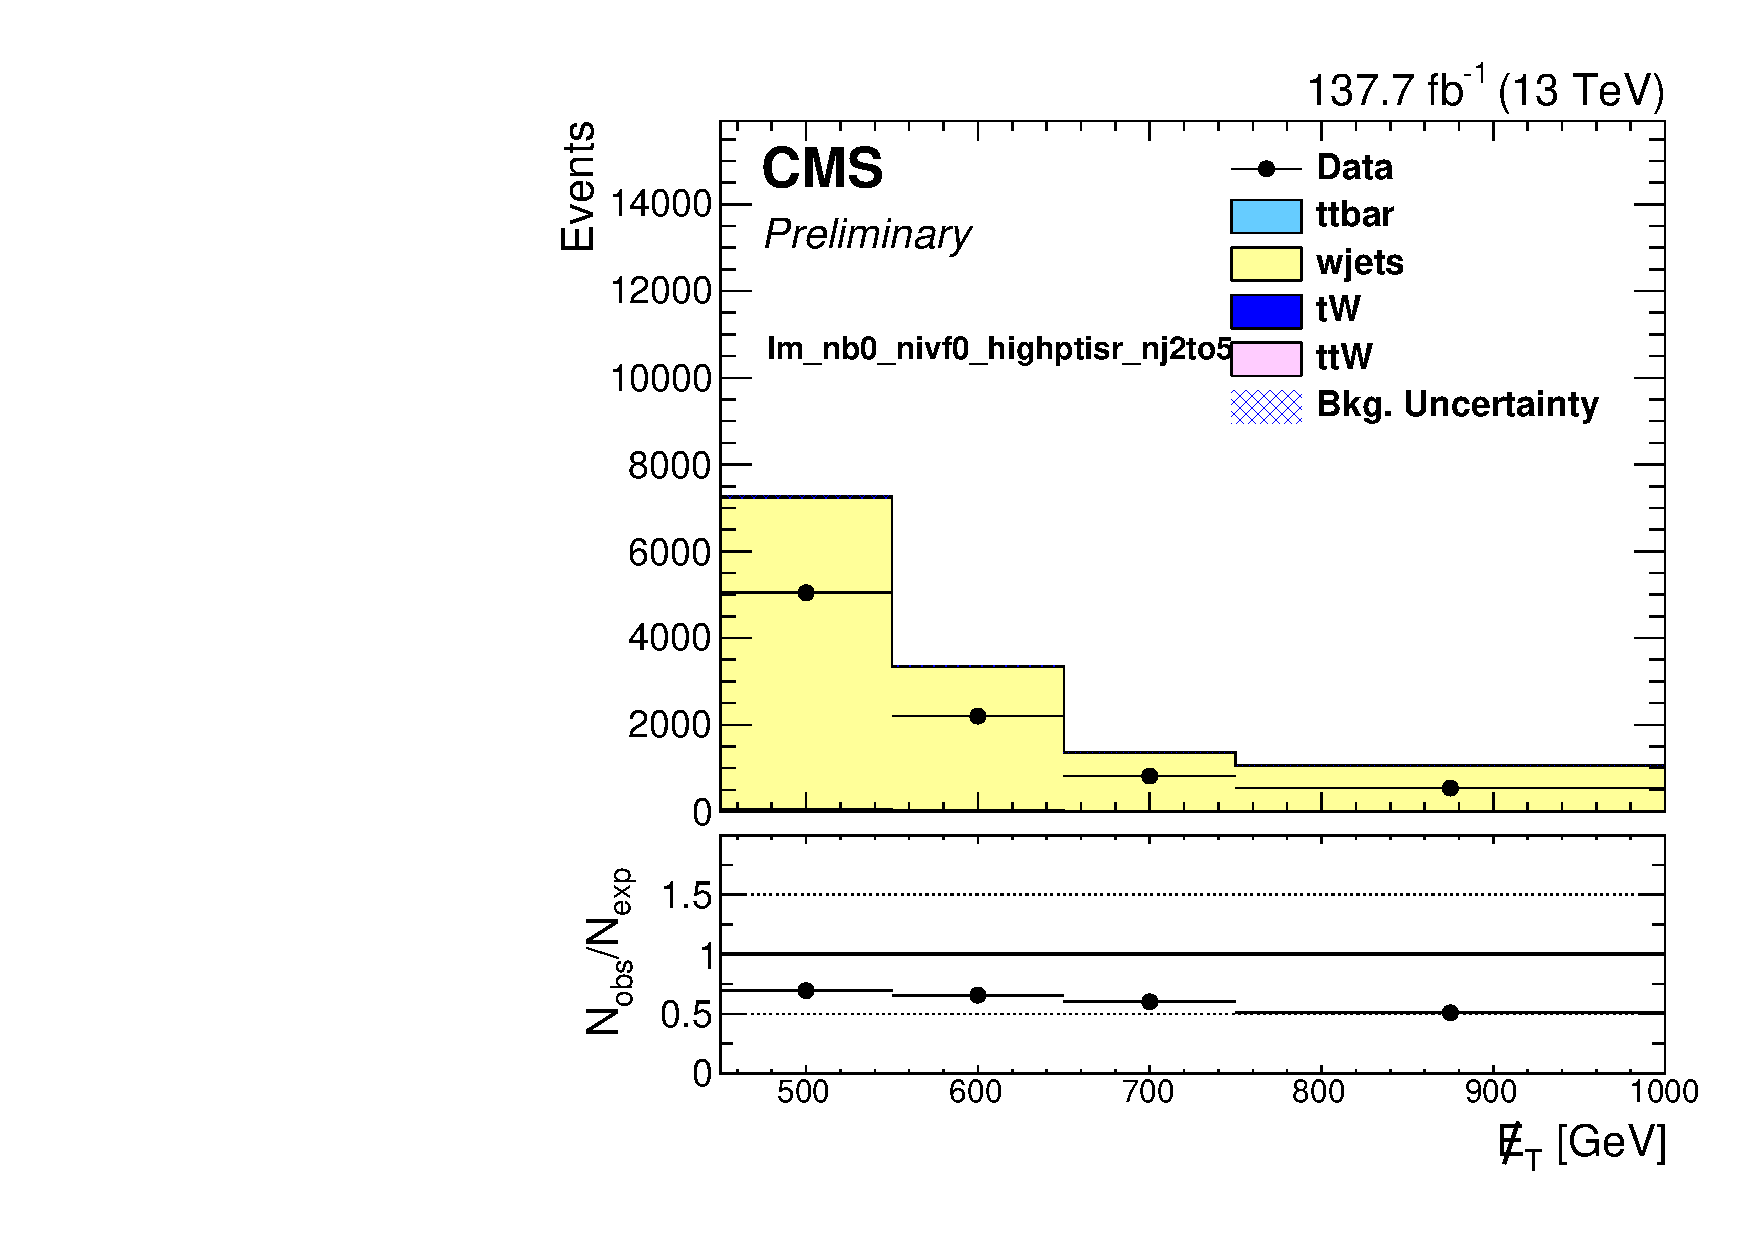
\includegraphics[width=0.49\textwidth]{lepcr_allEras/MET_pt_DataMC_lm_nb0_nivf0_highptisr_nj2to5__.pdf}
  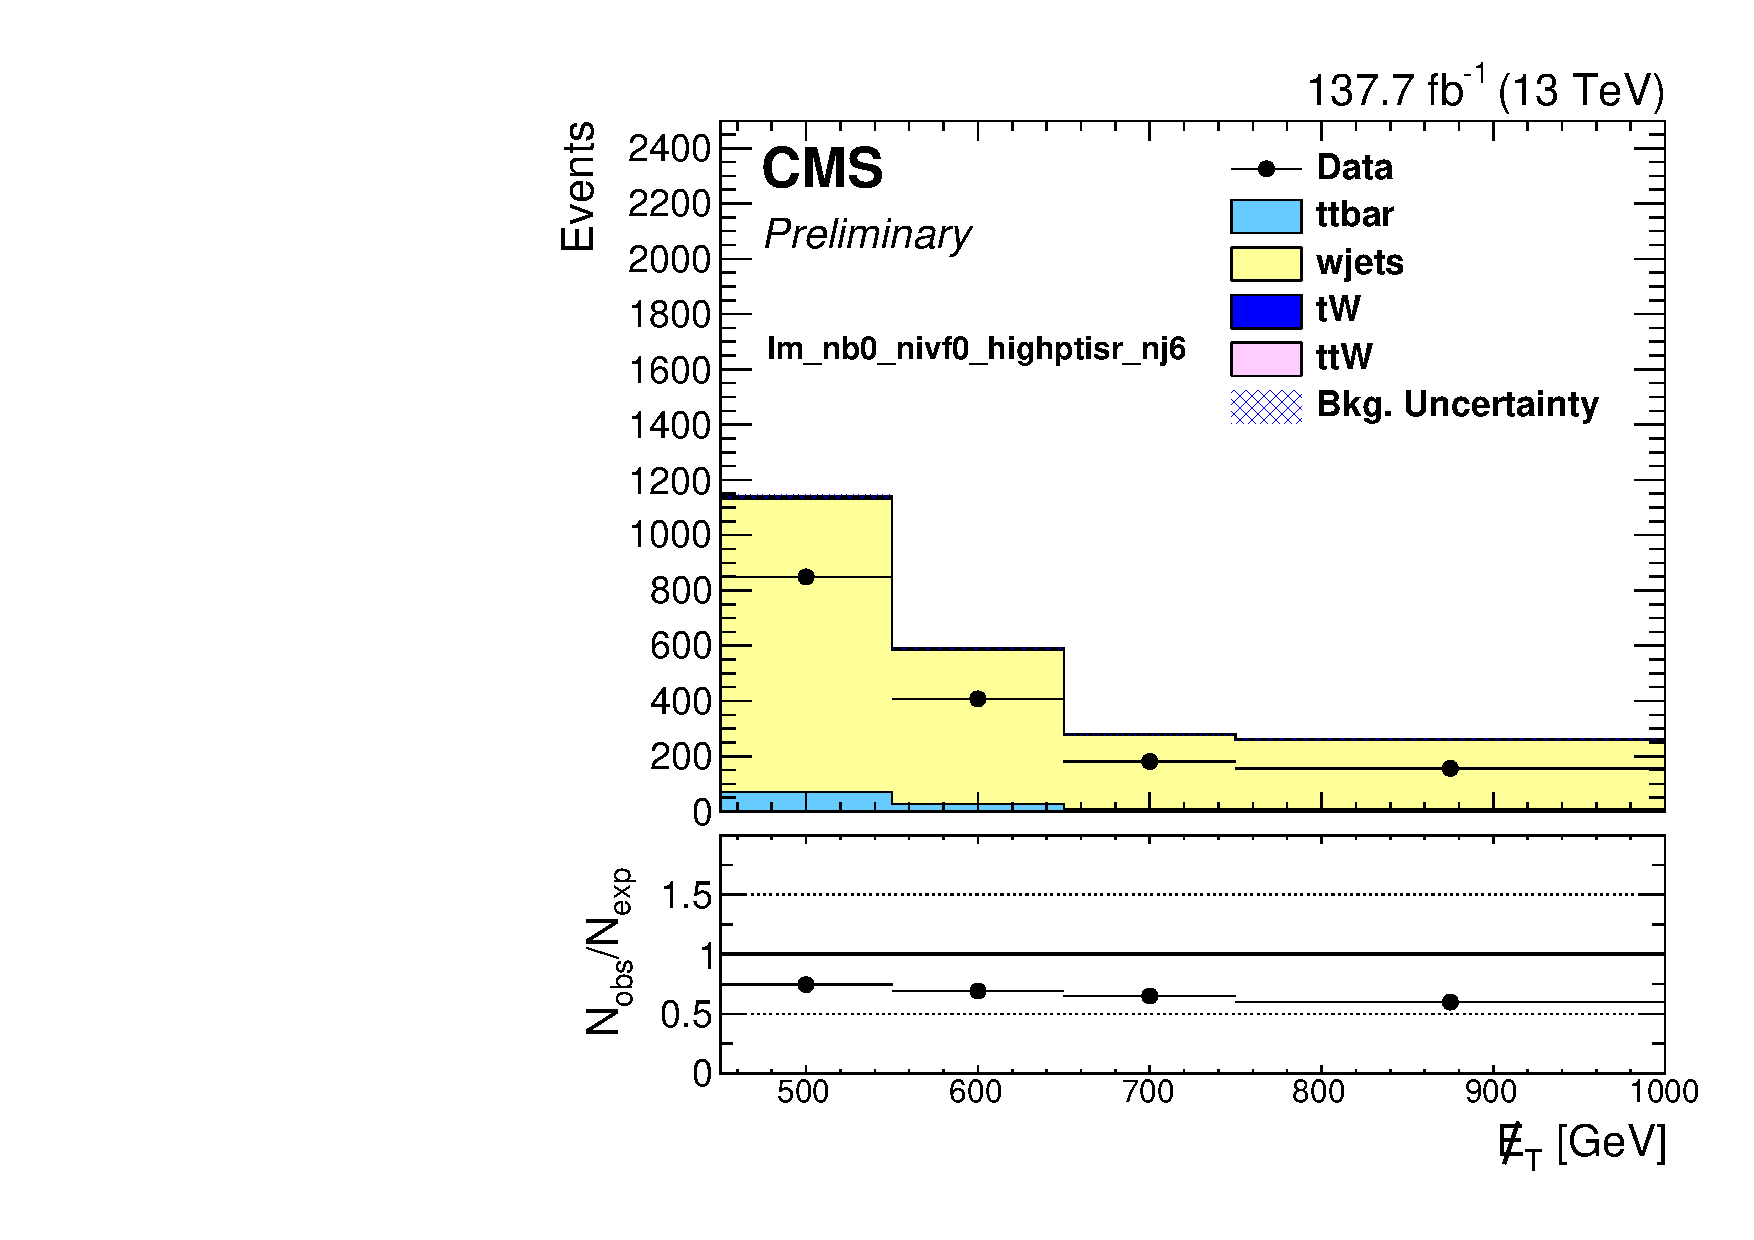
\includegraphics[width=0.49\textwidth]{lepcr_allEras/MET_pt_DataMC_lm_nb0_nivf0_highptisr_nj6__.pdf} \\
  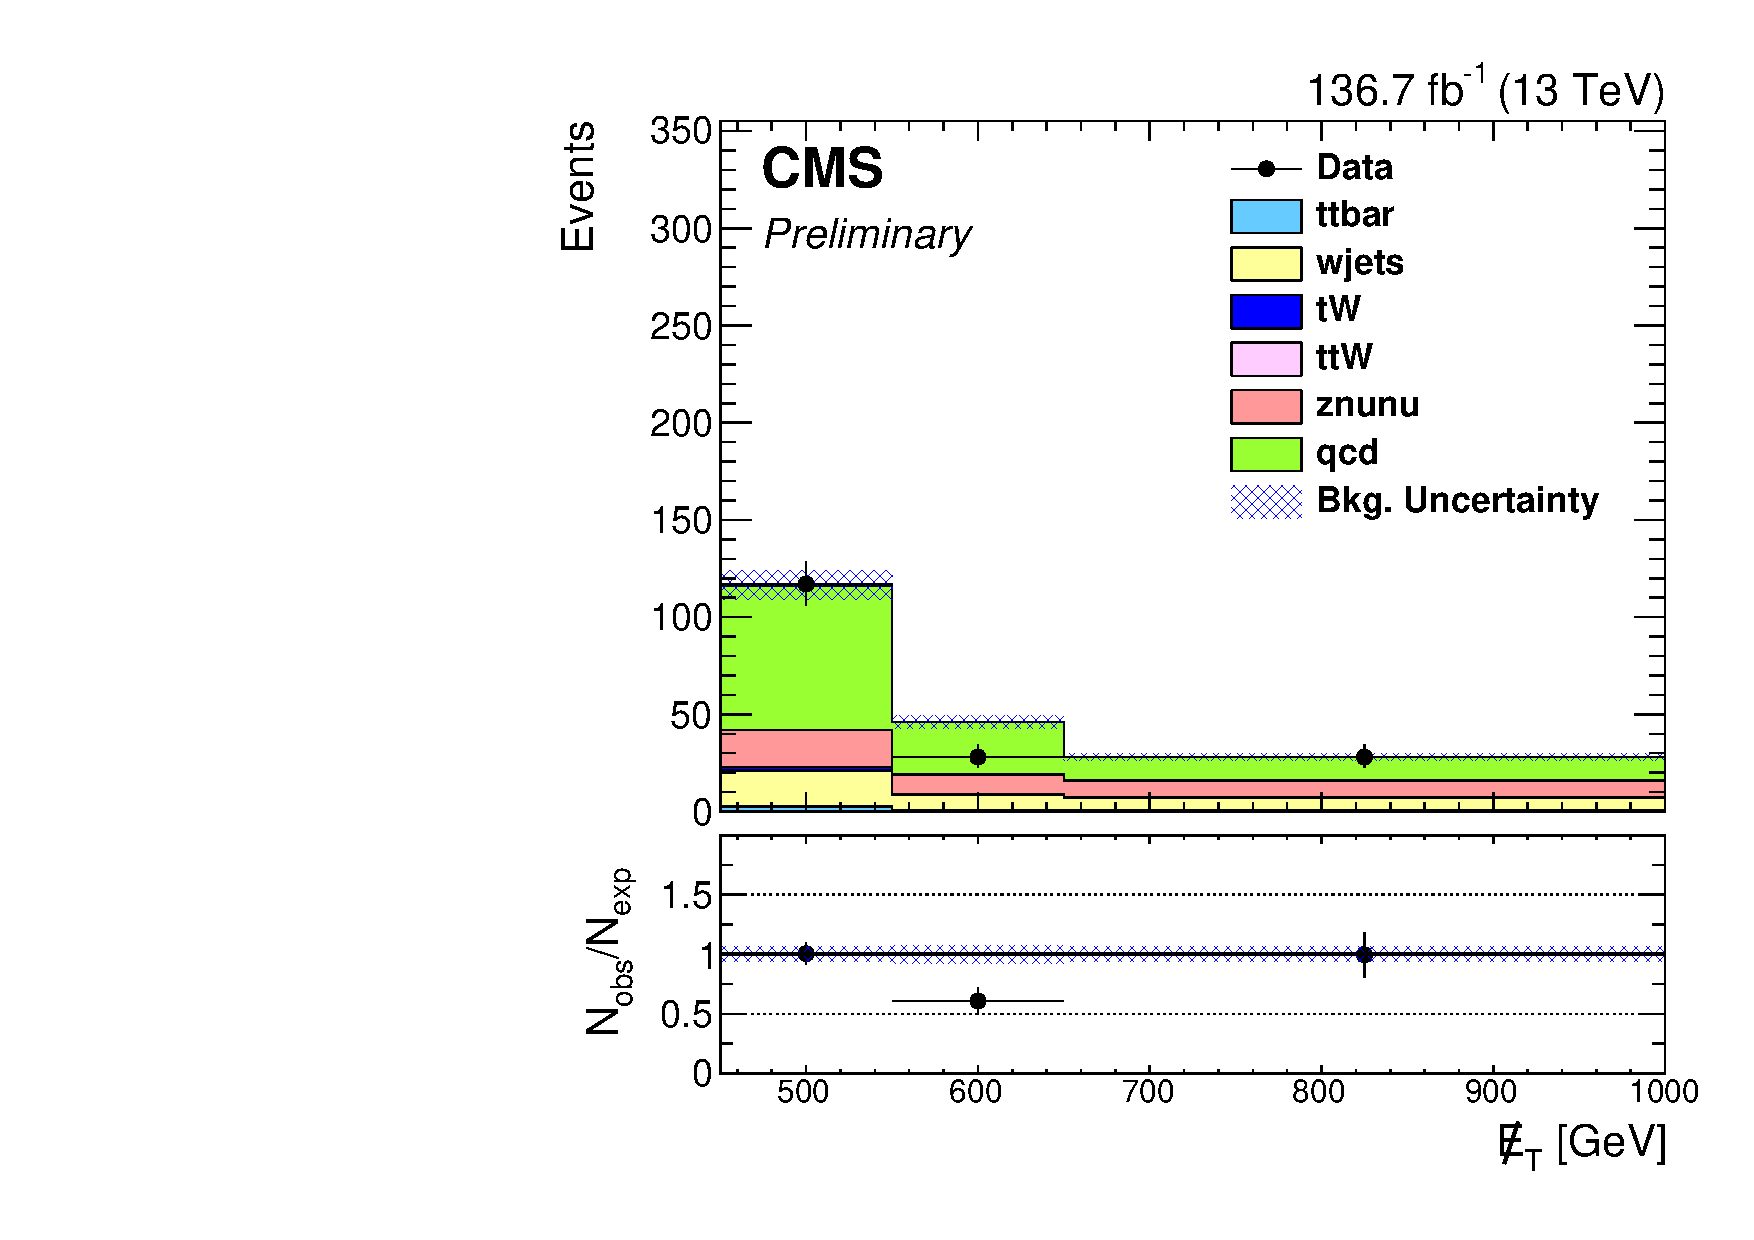
\includegraphics[width=0.49\textwidth]{lepcr_allEras/MET_pt_DataMC_lm_nb0_nivf1_highptisr_nj2to5__.pdf}
  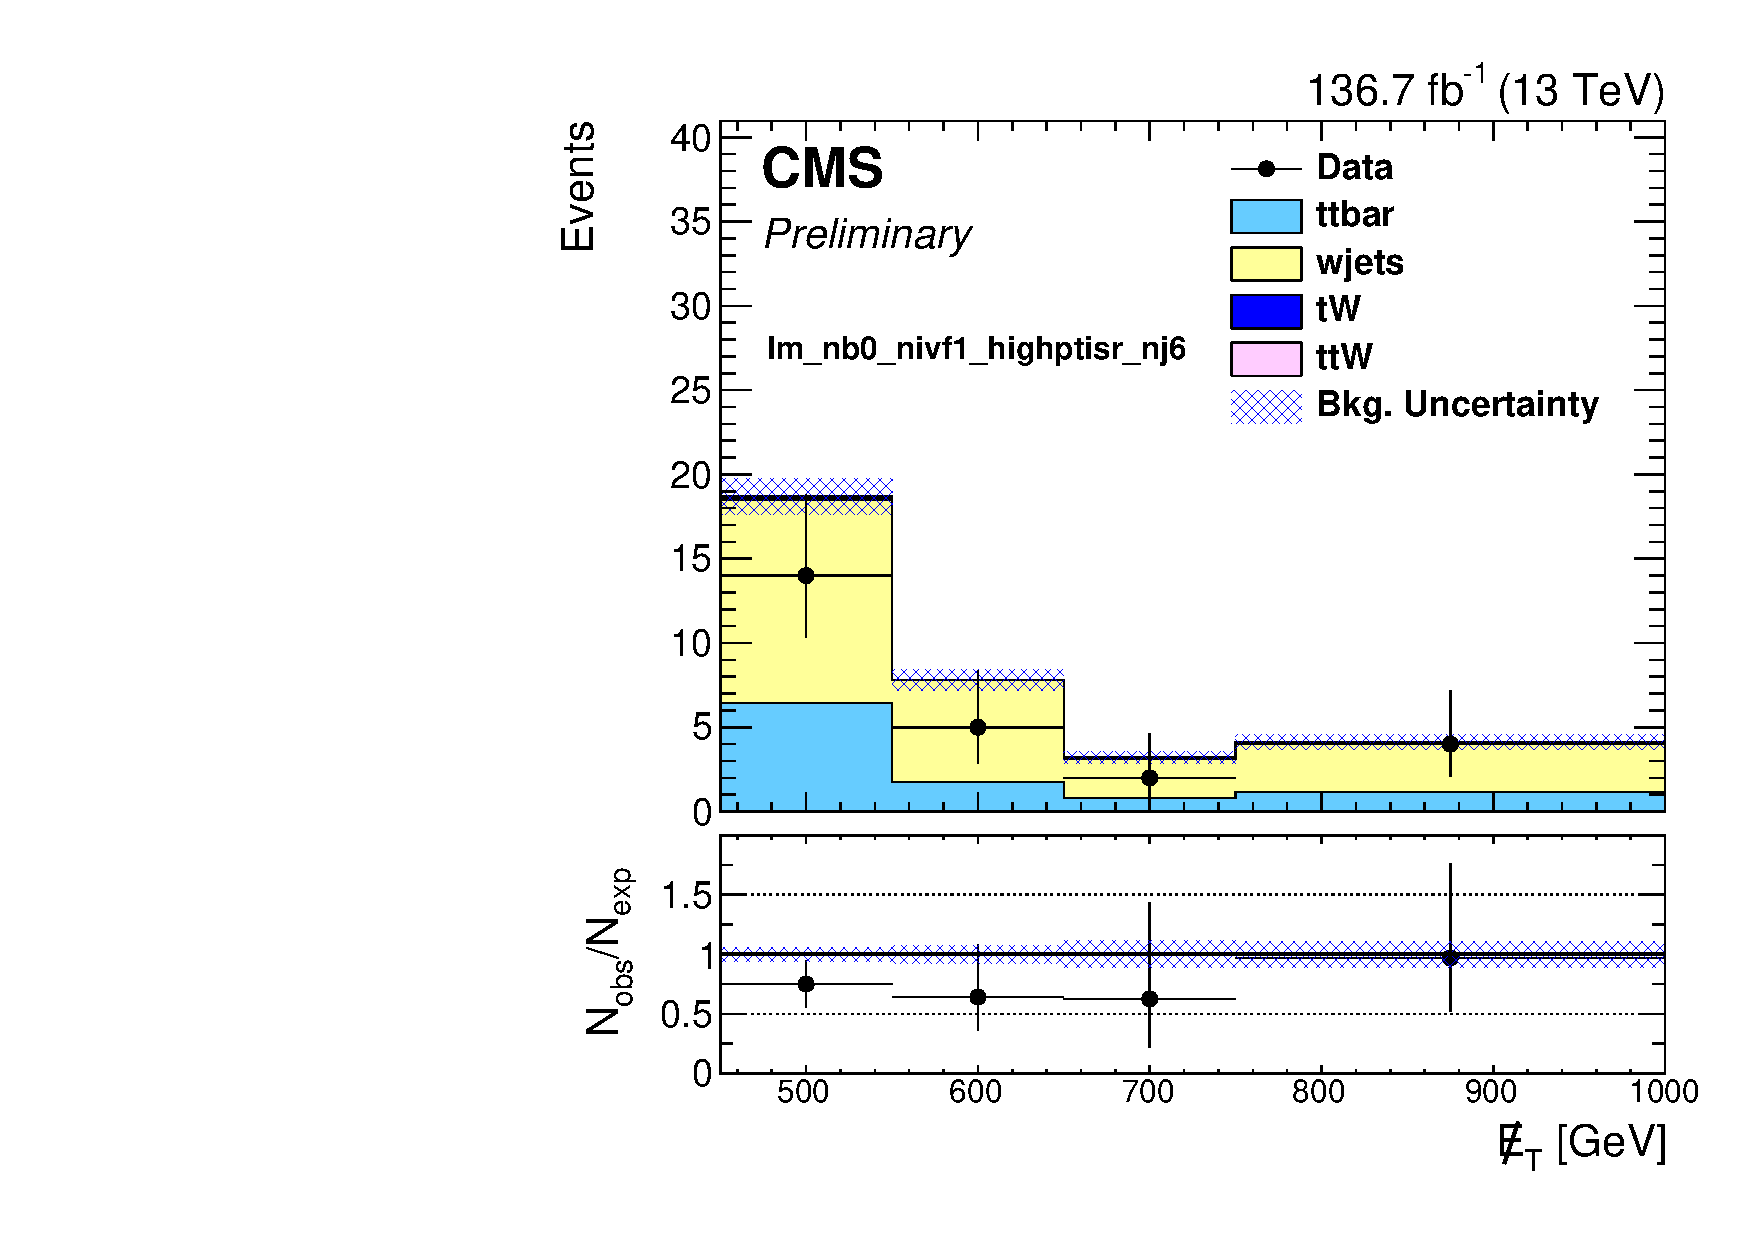
\includegraphics[width=0.49\textwidth]{lepcr_allEras/MET_pt_DataMC_lm_nb0_nivf1_highptisr_nj6__.pdf} \\
	\end{center}
	\caption[Lost Lepton LM Control Region $\nb=0$]{Comparison of the \met~distribution in the single-lepton sample after applying the low \dm~baseline selection in the $\nb=0$ region. Data and simulation are represented by the black points and stacked histograms, respectively. The error bars on the ratio of observed data to simulation correspond to the data statistical uncertainty and the shaded blue band represents the statistical uncertainty on the simulation. These regions are included with the search regions in the simultaneous fit for the signal extraction in order to estimate the LL contribution.
	 }
	\label{fig:llb-1lcr-datavsmc-lm-nb0}
\end{figure}
\begin{figure}[!h]
	\begin{center}  
		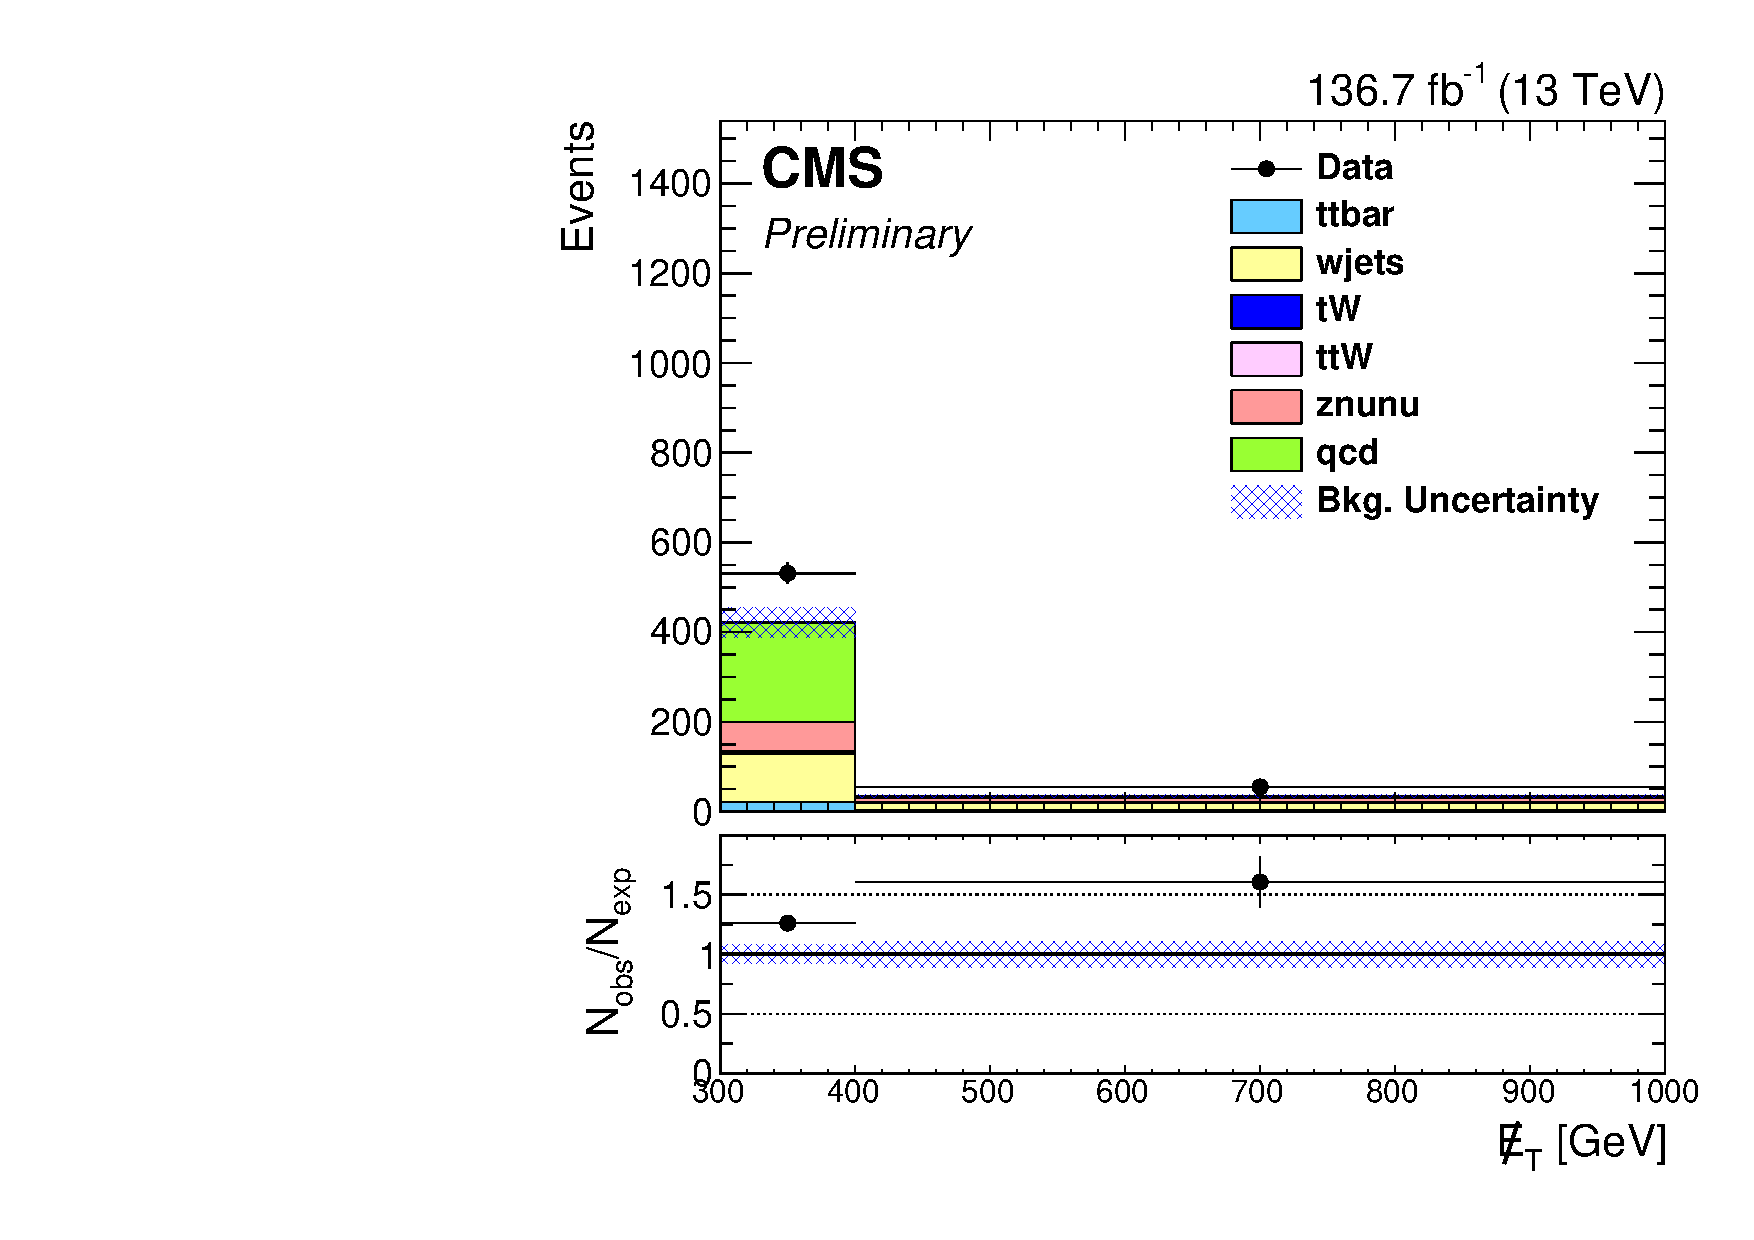
\includegraphics[width=0.32\textwidth]{lepcr_allEras/MET_pt_DataMC_lm_nb1_nivf0_lowmtb_lowptisr_lowptb__.pdf}
		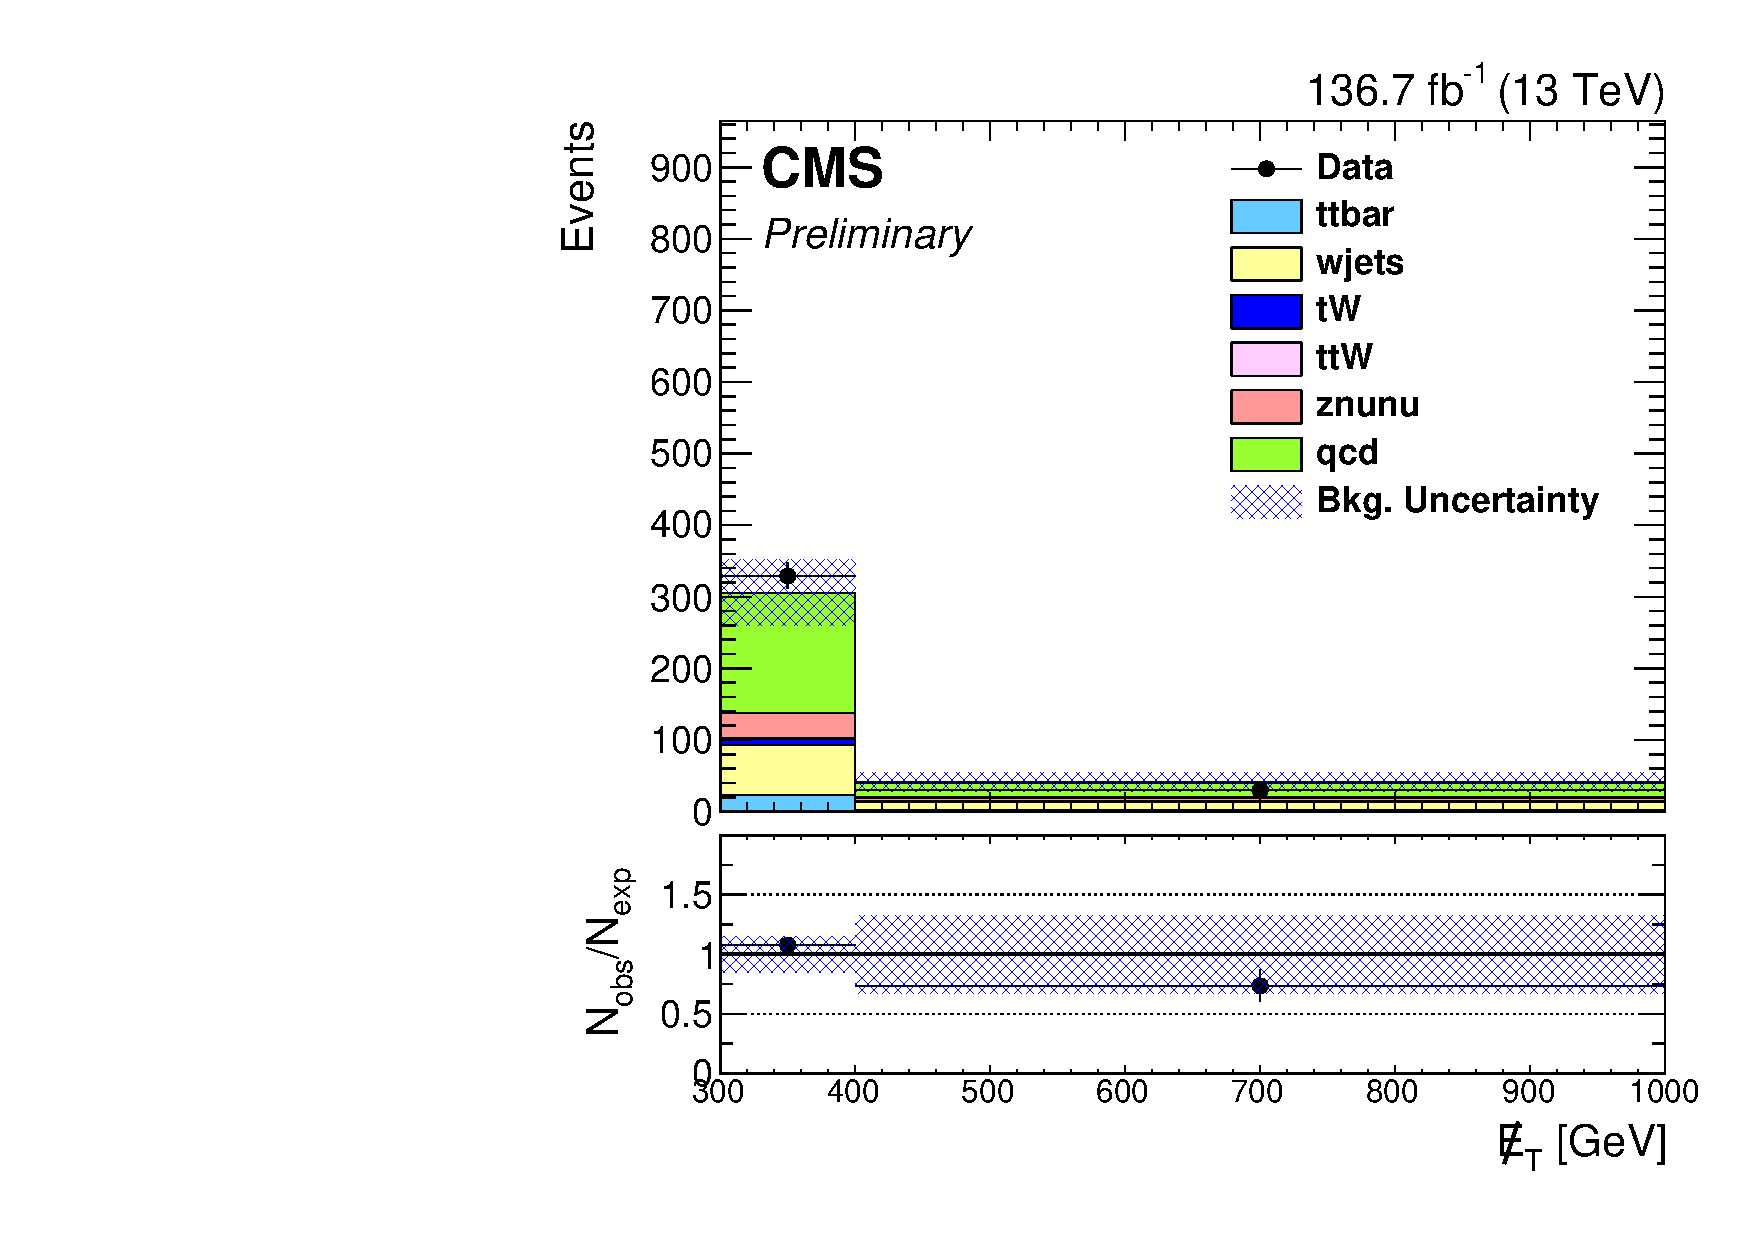
\includegraphics[width=0.32\textwidth]{lepcr_allEras/MET_pt_DataMC_lm_nb1_nivf0_lowmtb_lowptisr_medptb__.pdf} \\
		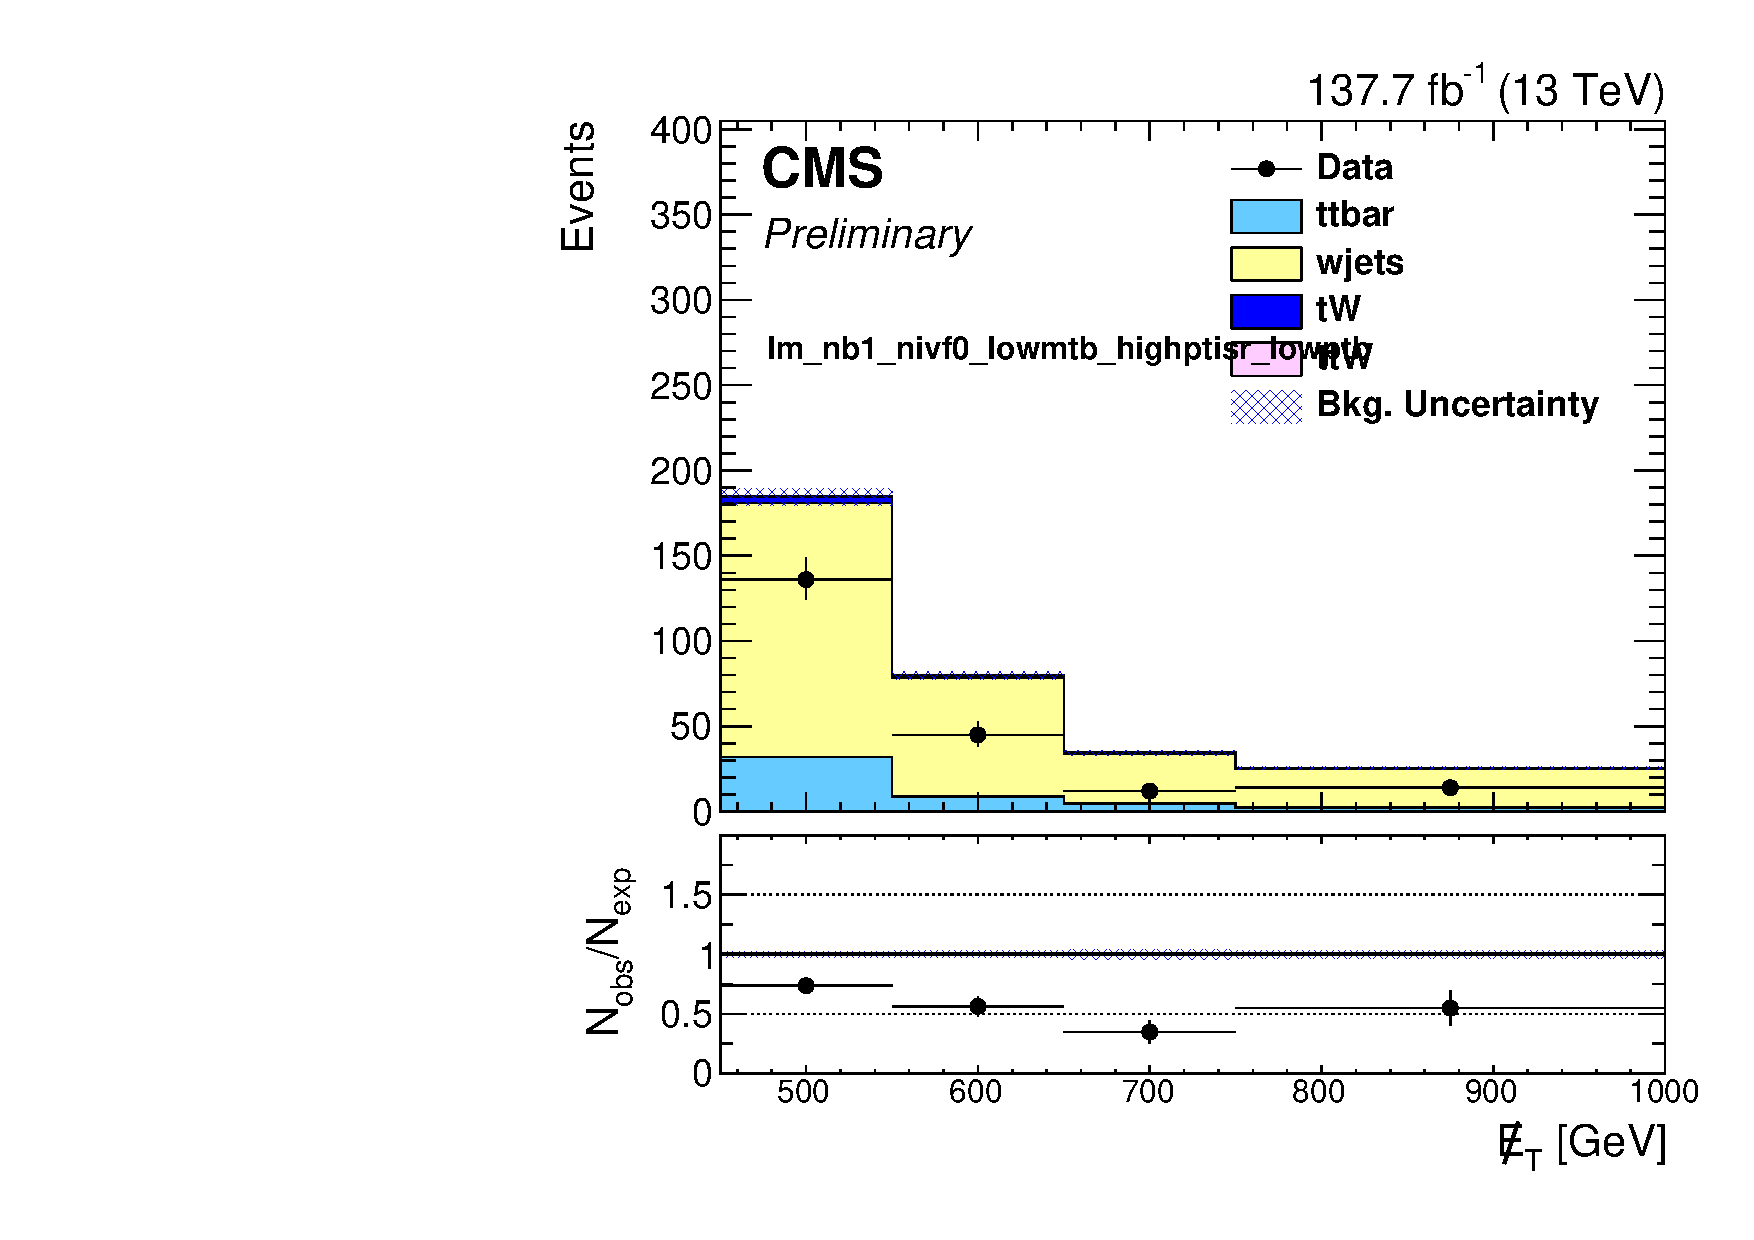
\includegraphics[width=0.32\textwidth]{lepcr_allEras/MET_pt_DataMC_lm_nb1_nivf0_lowmtb_highptisr_lowptb__.pdf}
		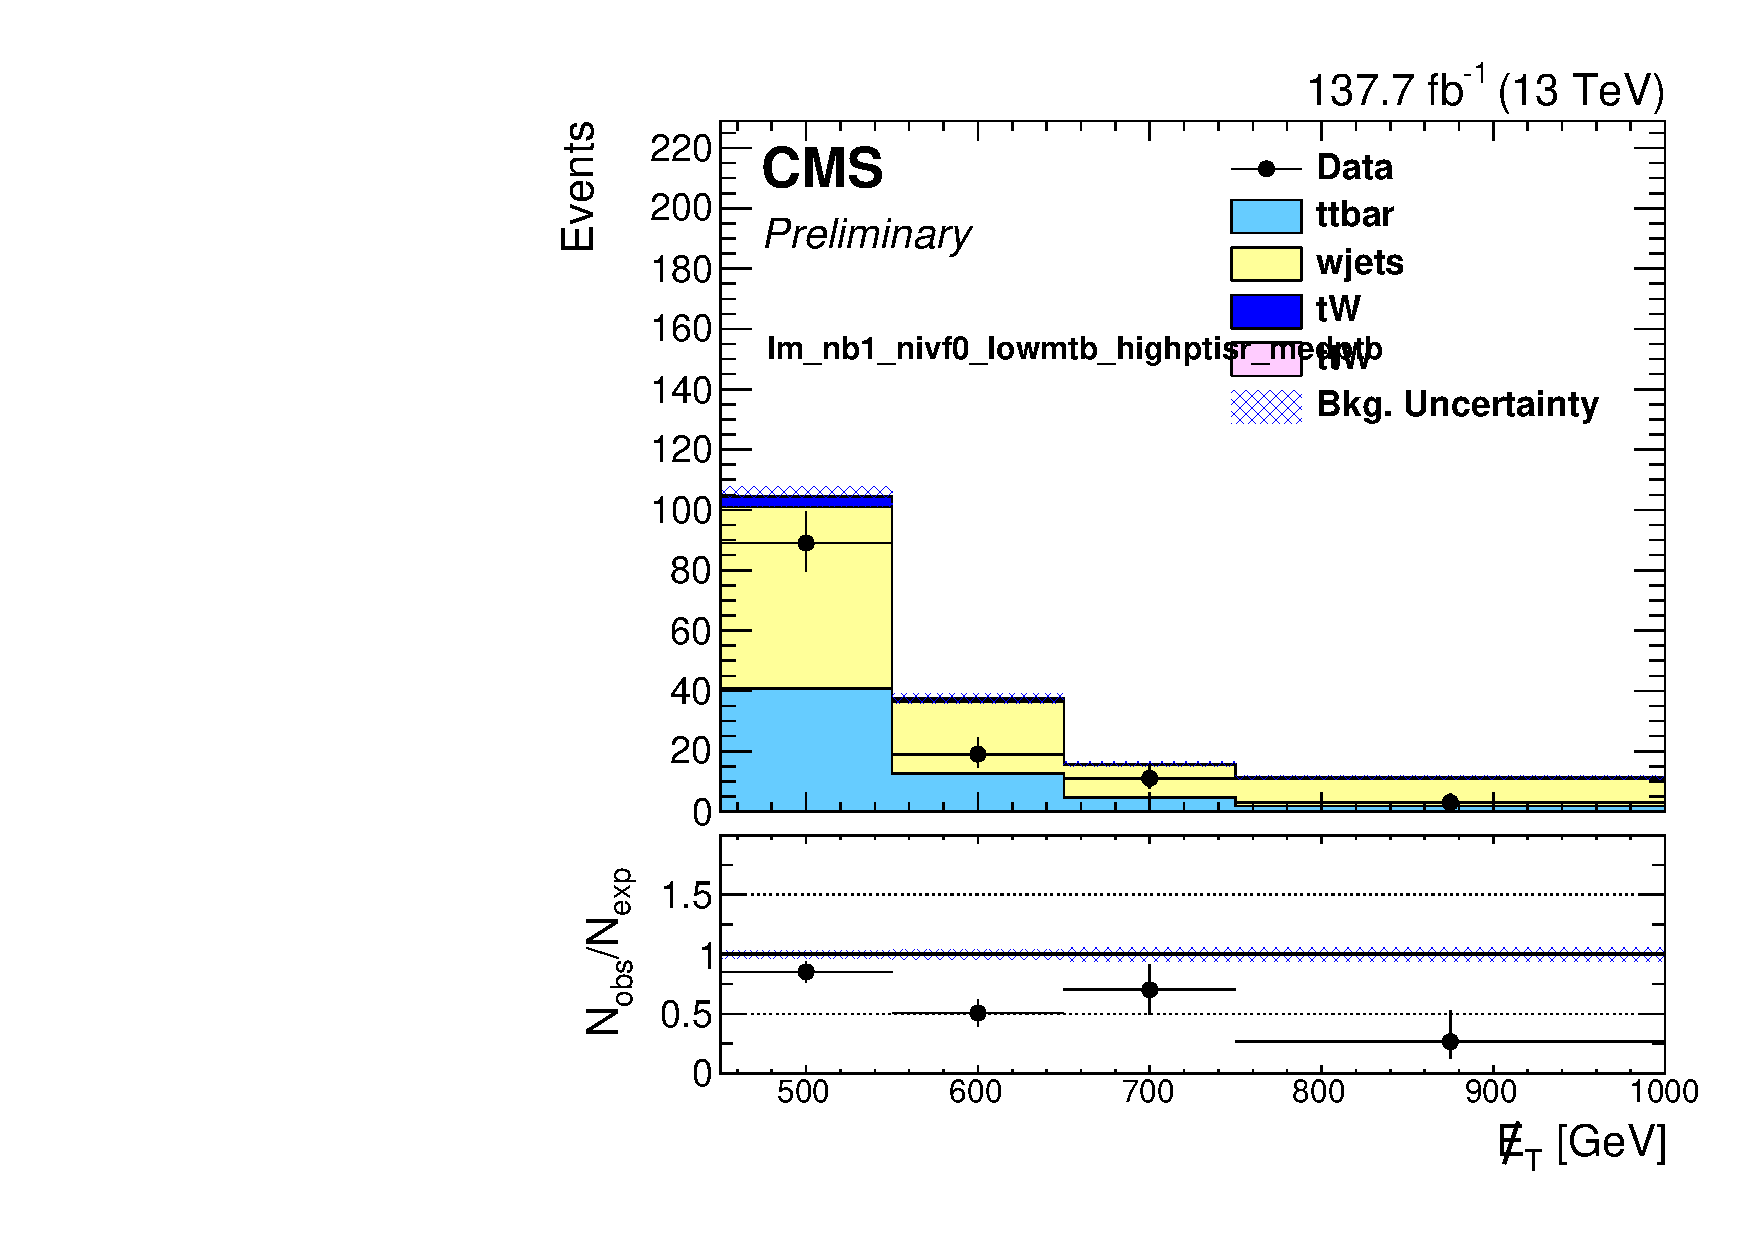
\includegraphics[width=0.32\textwidth]{lepcr_allEras/MET_pt_DataMC_lm_nb1_nivf0_lowmtb_highptisr_medptb__.pdf}
		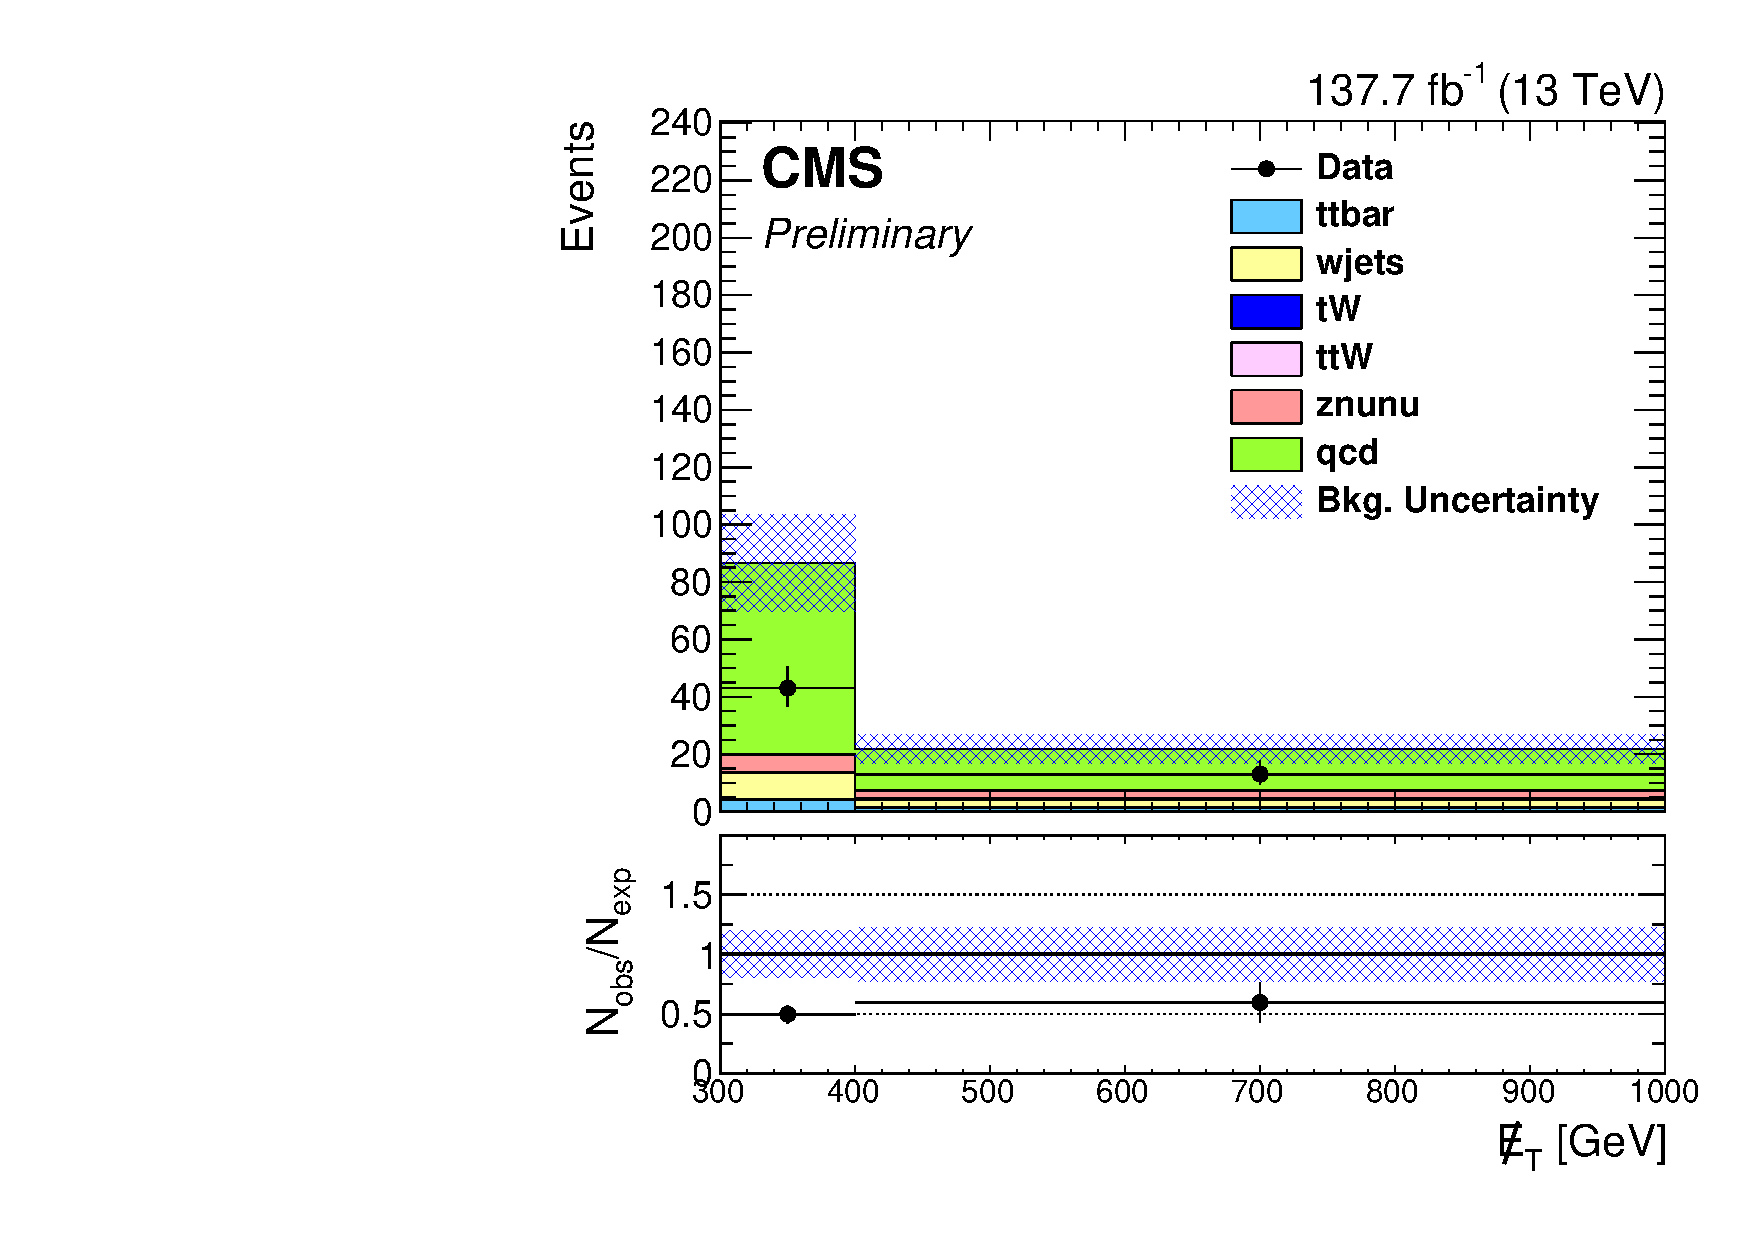
\includegraphics[width=0.32\textwidth]{lepcr_allEras/MET_pt_DataMC_lm_nb1_nivf1_lowmtb_lowptb__.pdf} \\
		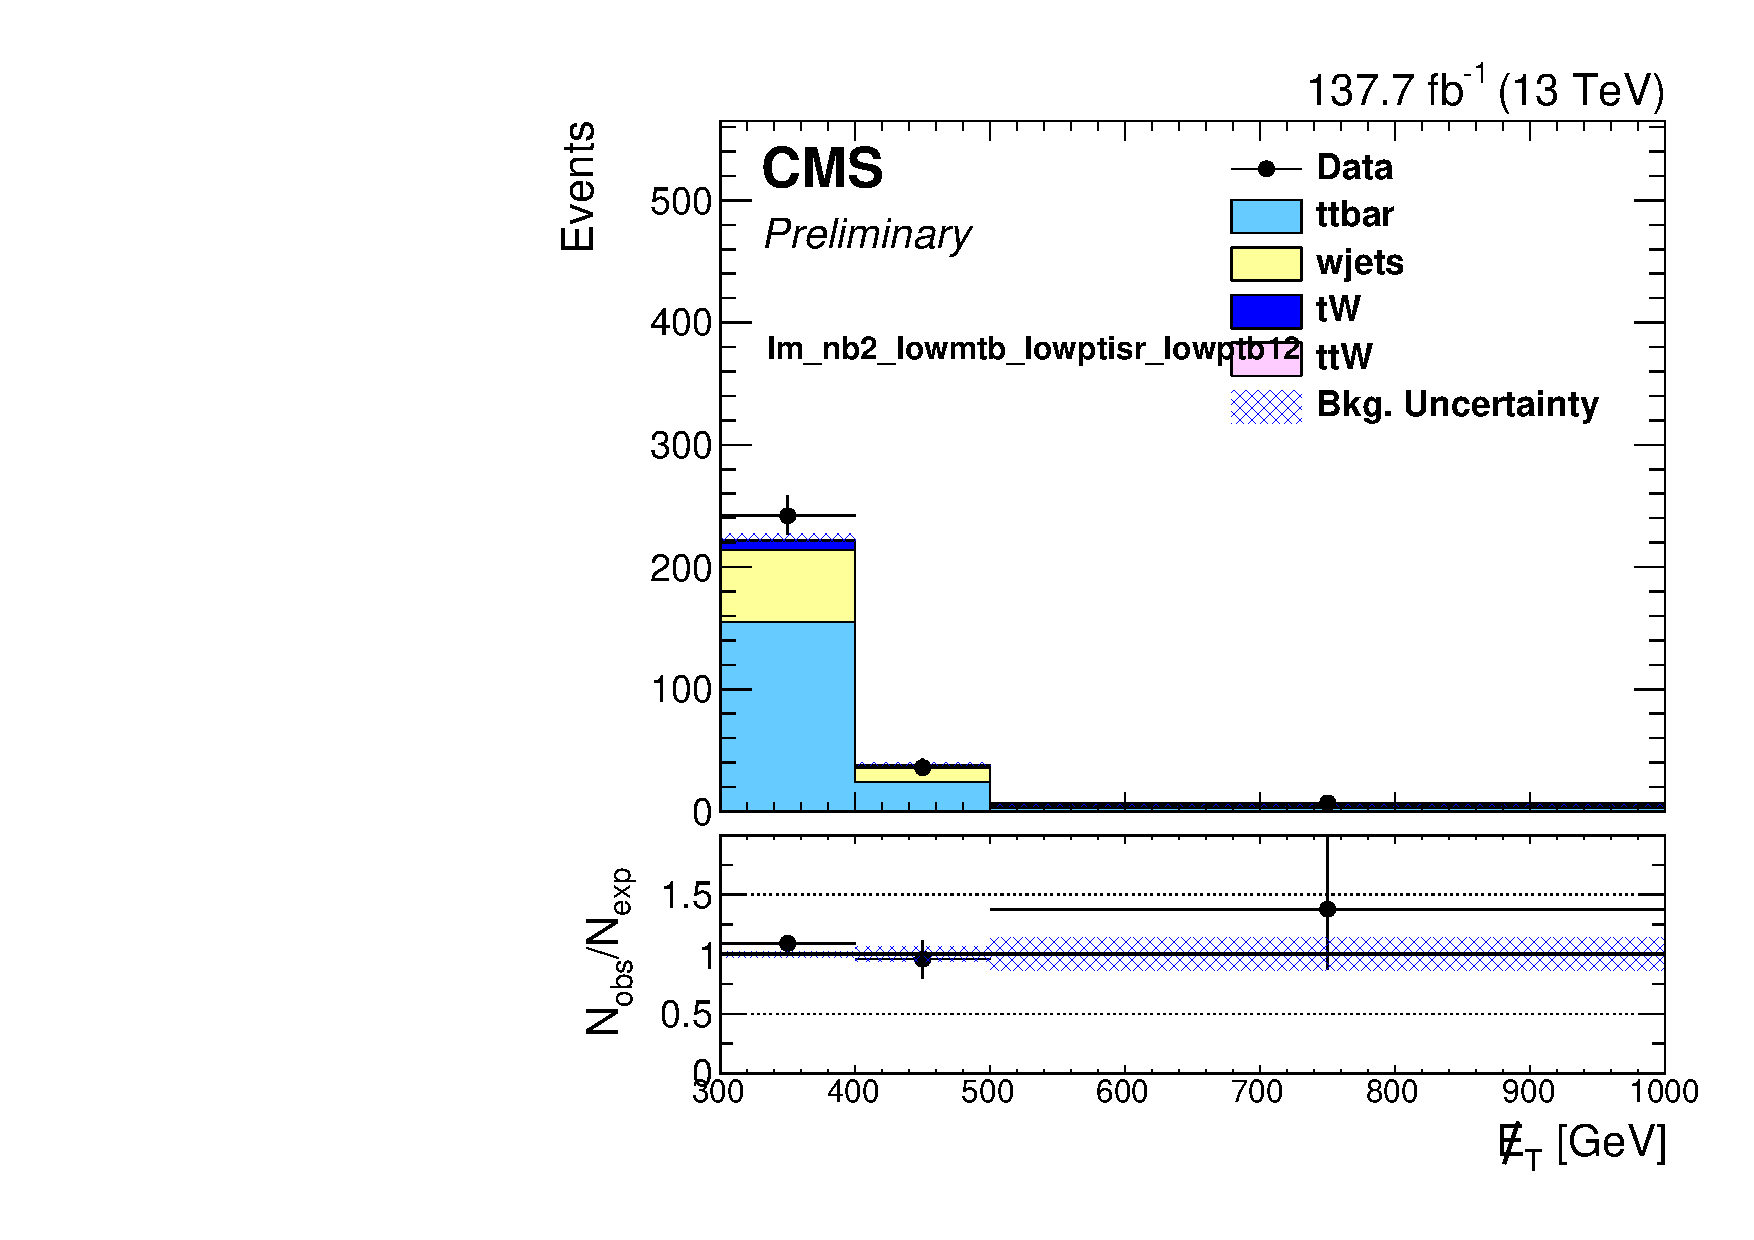
\includegraphics[width=0.32\textwidth]{lepcr_allEras/MET_pt_DataMC_lm_nb2_lowmtb_lowptisr_lowptb12__.pdf} 
		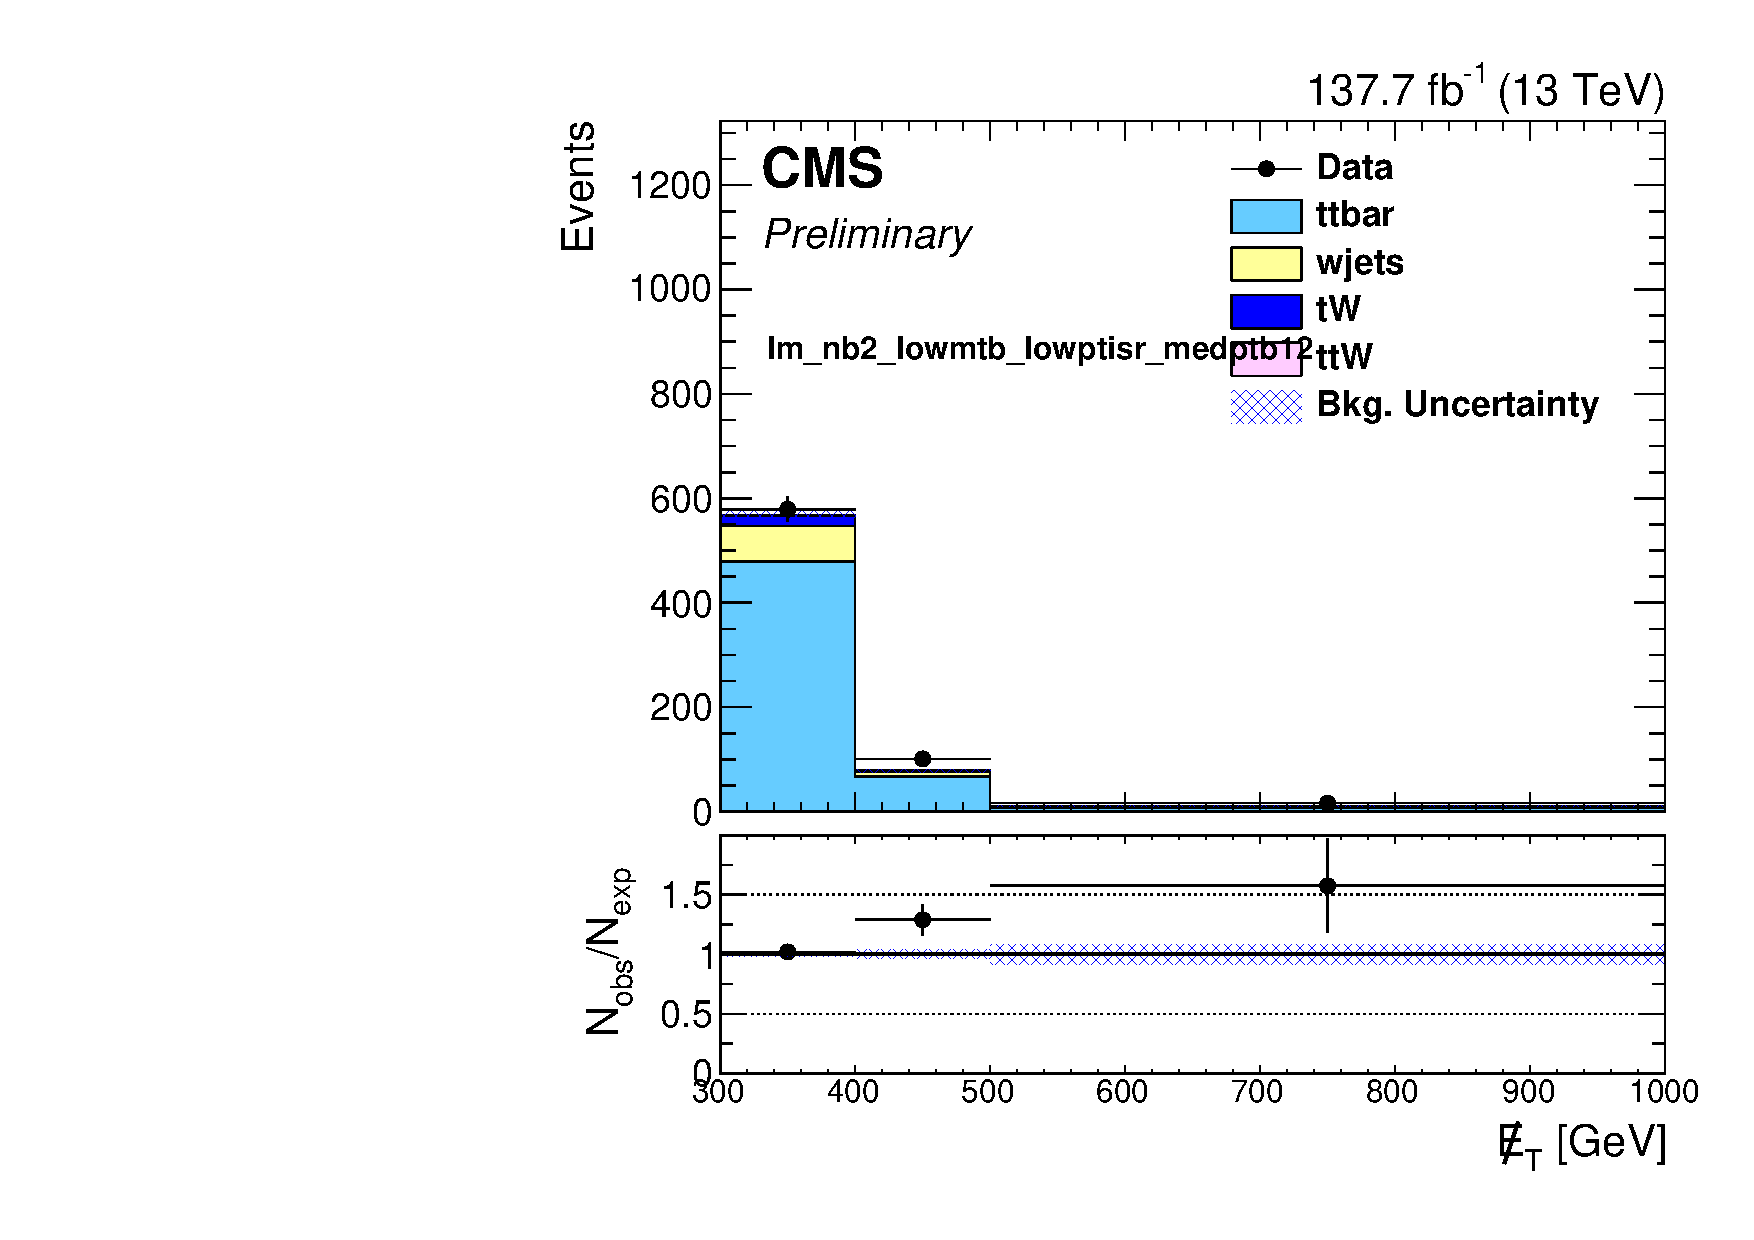
\includegraphics[width=0.32\textwidth]{lepcr_allEras/MET_pt_DataMC_lm_nb2_lowmtb_lowptisr_medptb12__.pdf}
		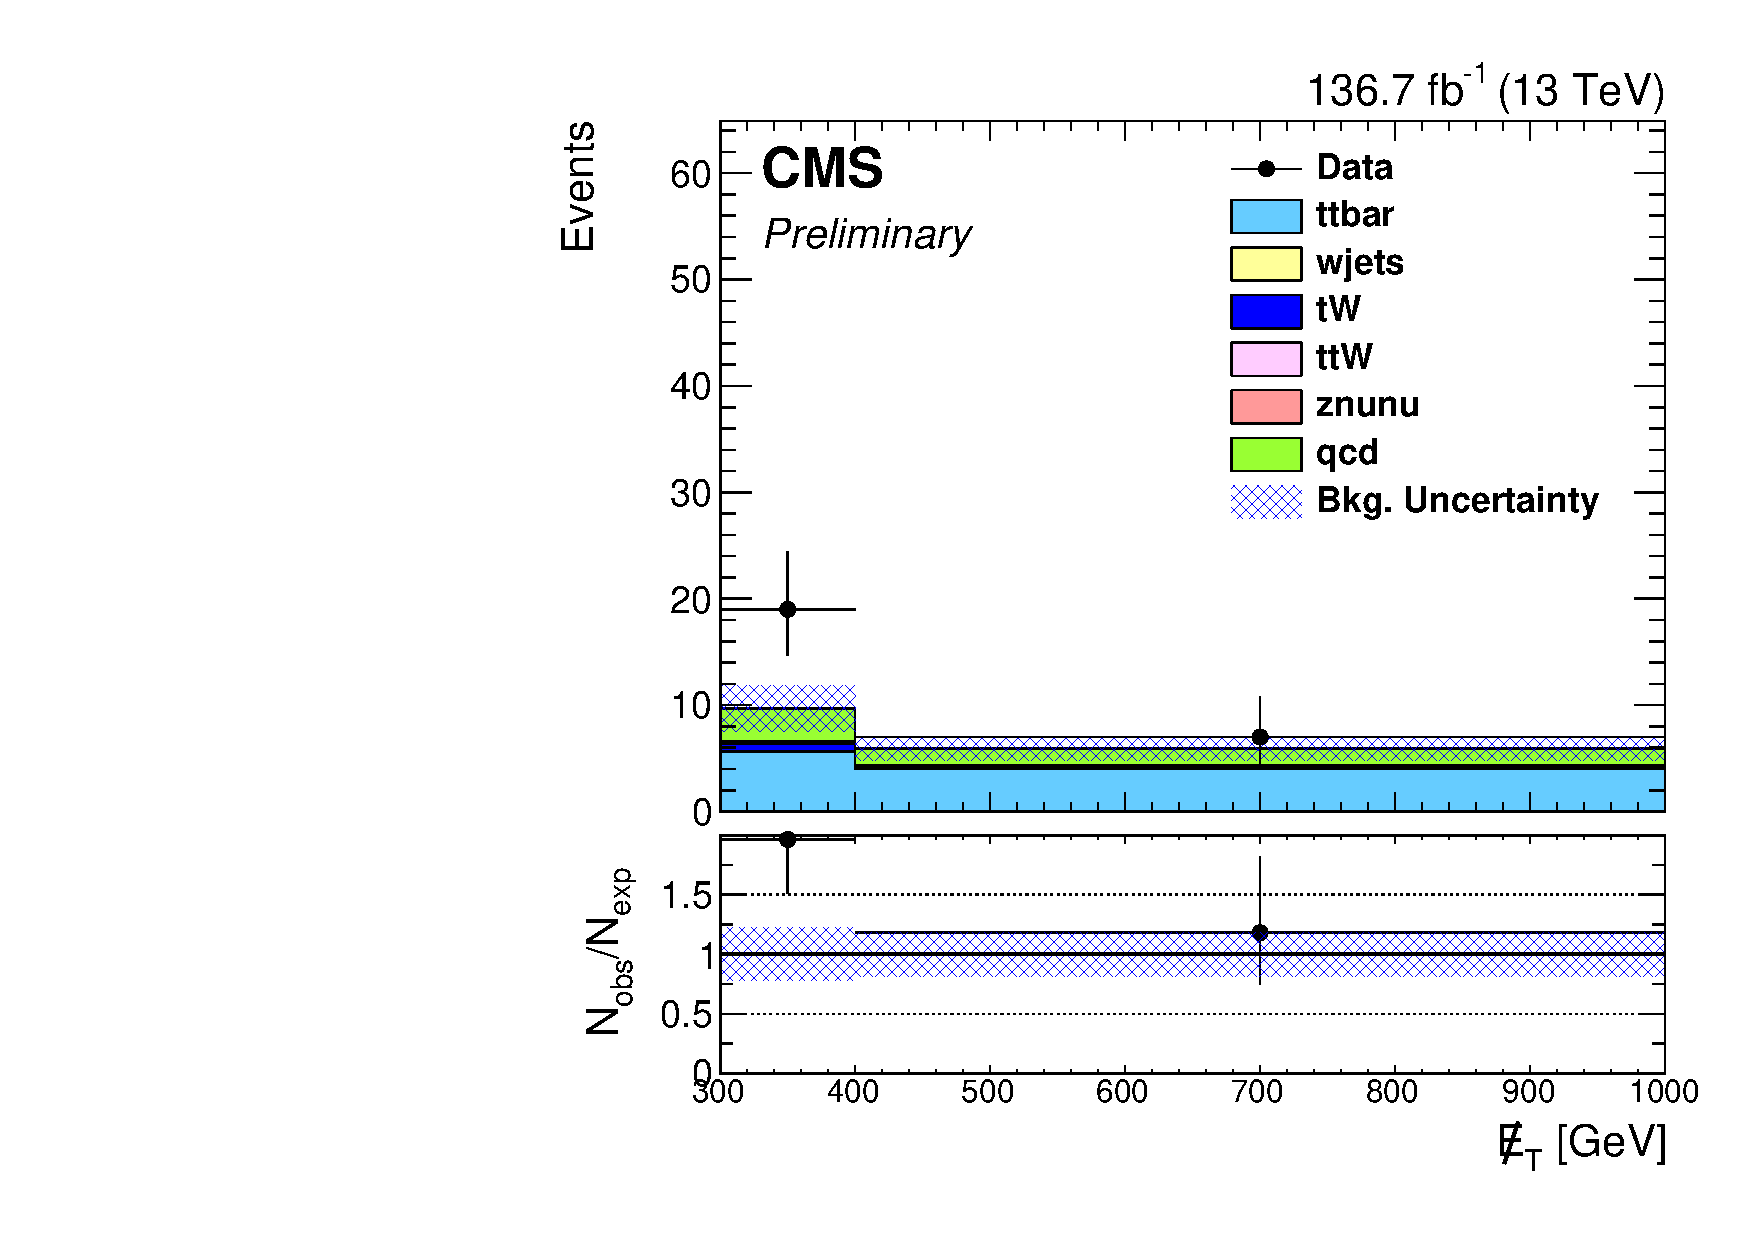
\includegraphics[width=0.32\textwidth]{lepcr_allEras/MET_pt_DataMC_lm_nb2_lowmtb_lowptisr_highptb12_nj7__.pdf} \\
		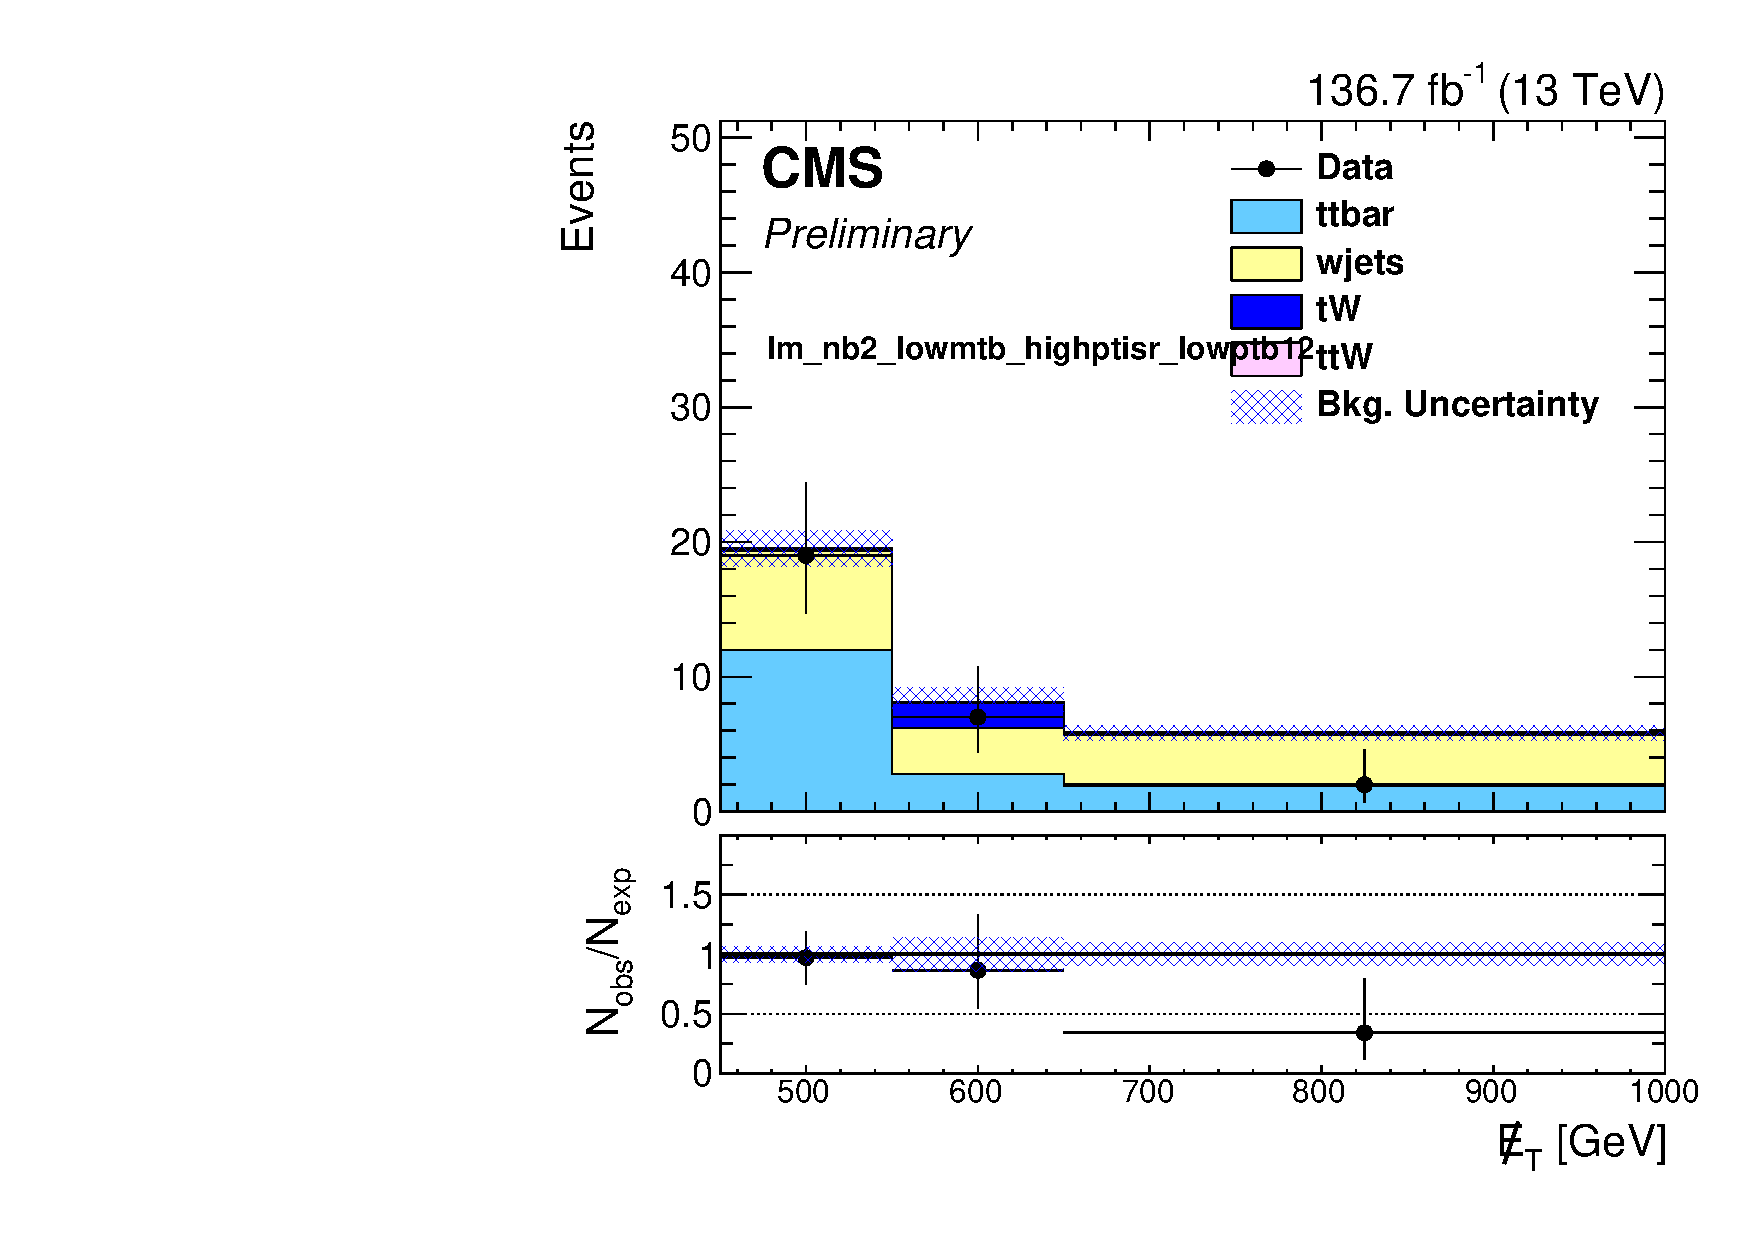
\includegraphics[width=0.32\textwidth]{lepcr_allEras/MET_pt_DataMC_lm_nb2_lowmtb_highptisr_lowptb12__.pdf} 
		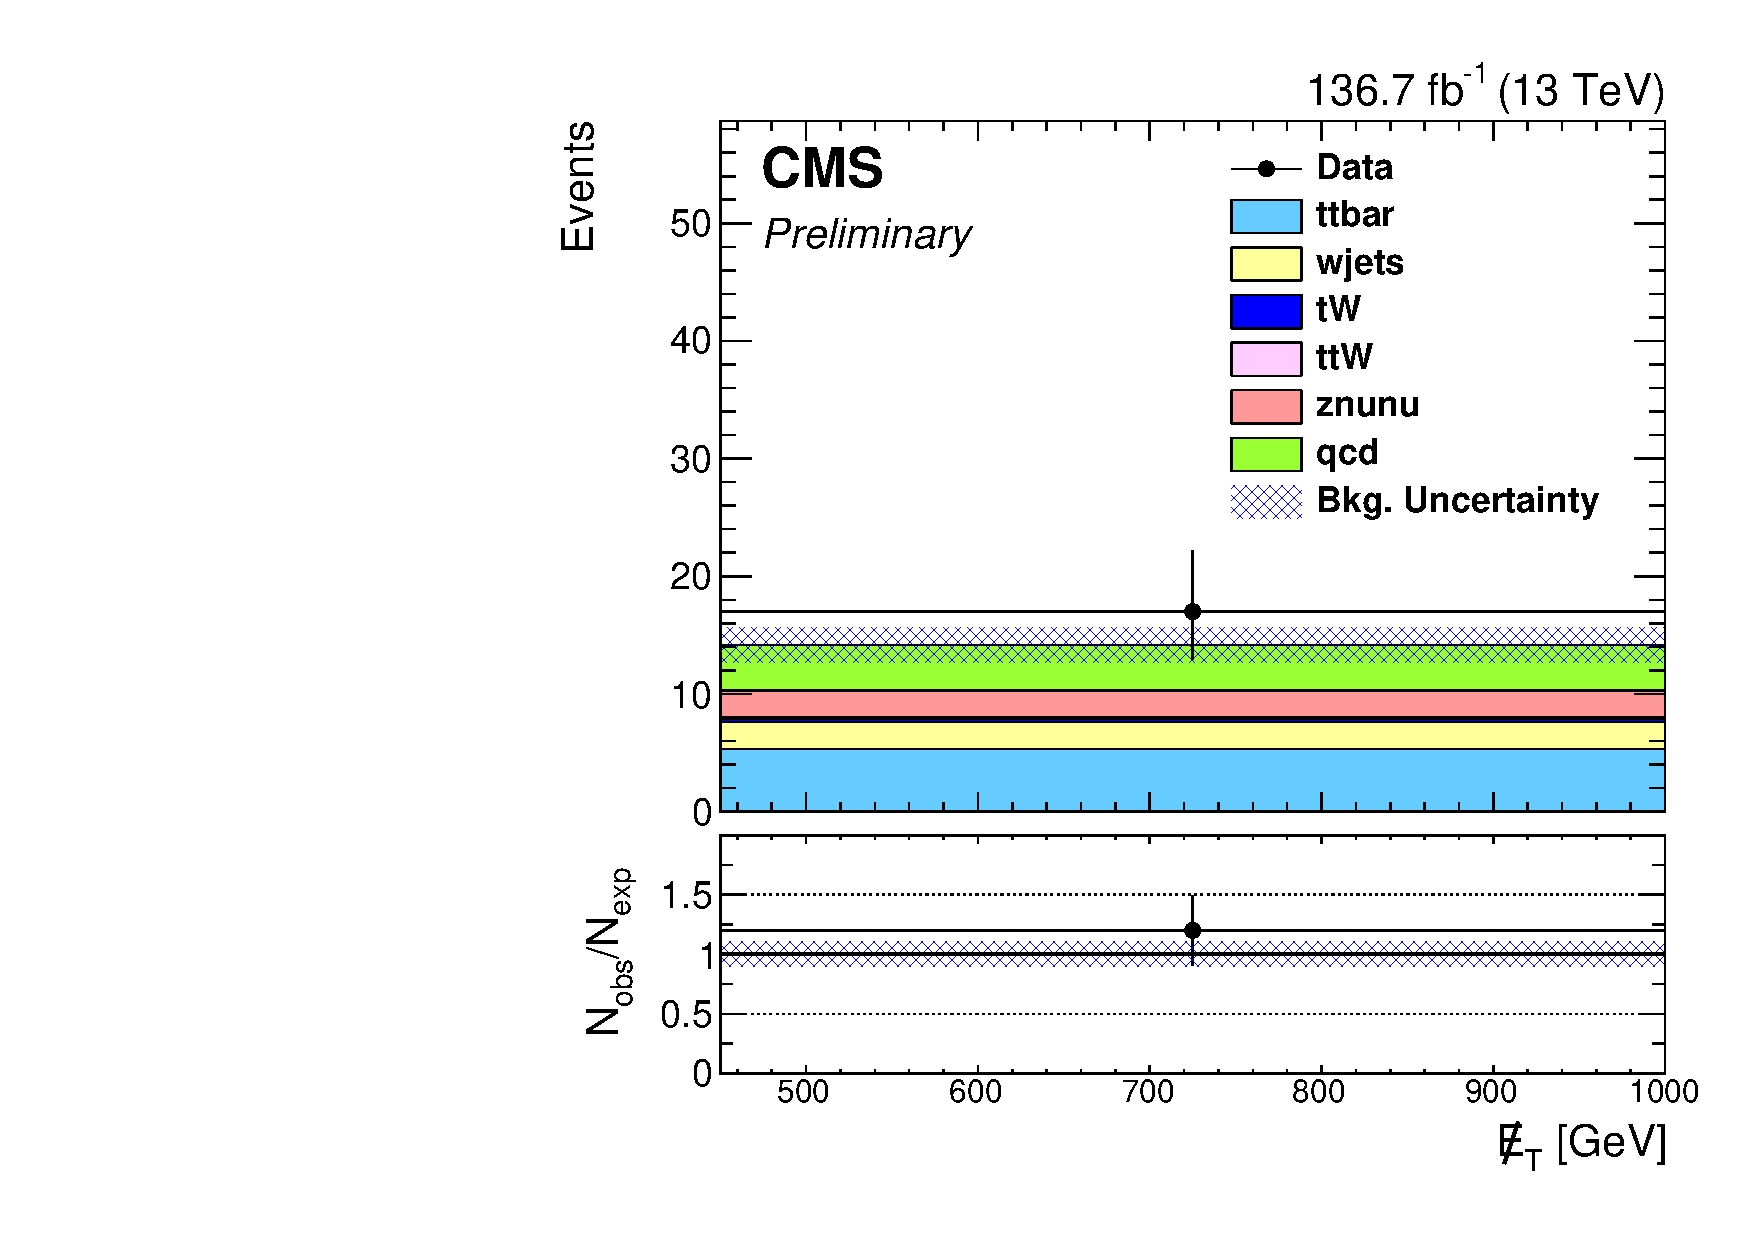
\includegraphics[width=0.32\textwidth]{lepcr_allEras/MET_pt_DataMC_lm_nb2_lowmtb_highptisr_medptb12__.pdf}
		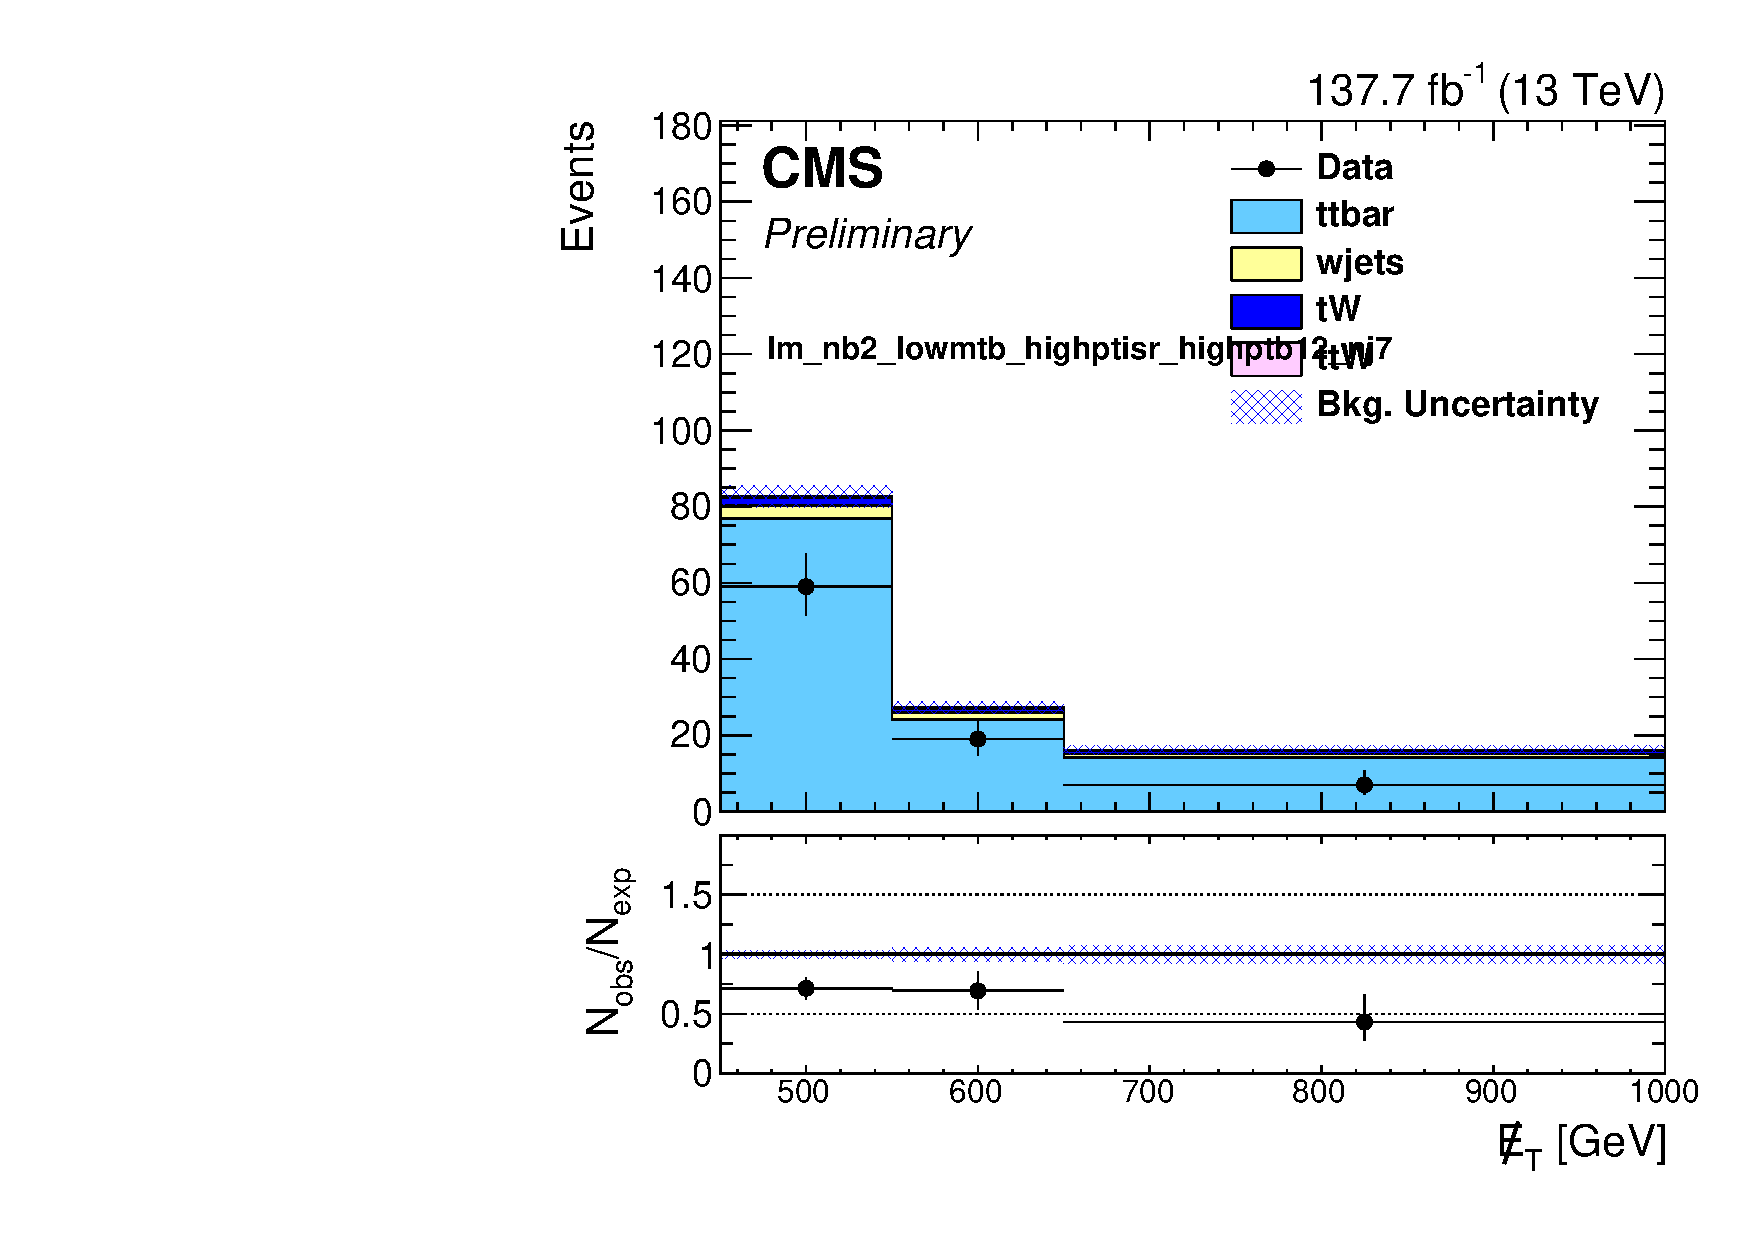
\includegraphics[width=0.32\textwidth]{lepcr_allEras/MET_pt_DataMC_lm_nb2_lowmtb_highptisr_highptb12_nj7__.pdf} \\
	\end{center}
	\caption[Lost Lepton LM Control Region $\nb=1$]{Comparison of the \met~distribution in the single-lepton sample after applying the low \dm~baseline selection. Two top rows: Events with $\nb=1$; Two bottom rows: Events with $\nb \geq2$;  Data and simulation are represented by the black points and stacked histograms, respectively. The error bars on the ratio of observed data to simulation correspond to the data statistical uncertainty and the shaded blue band represents the statistical uncertainty on the simulation. These regions are included with the search regions in the simultaneous fit for the signal extraction in order to estimate the LL contribution.
	 }
	\label{fig:llb-1lcr-datavsmc-lm-nb1}
\end{figure}

\begin{figure}[!htb]
	\begin{center}
  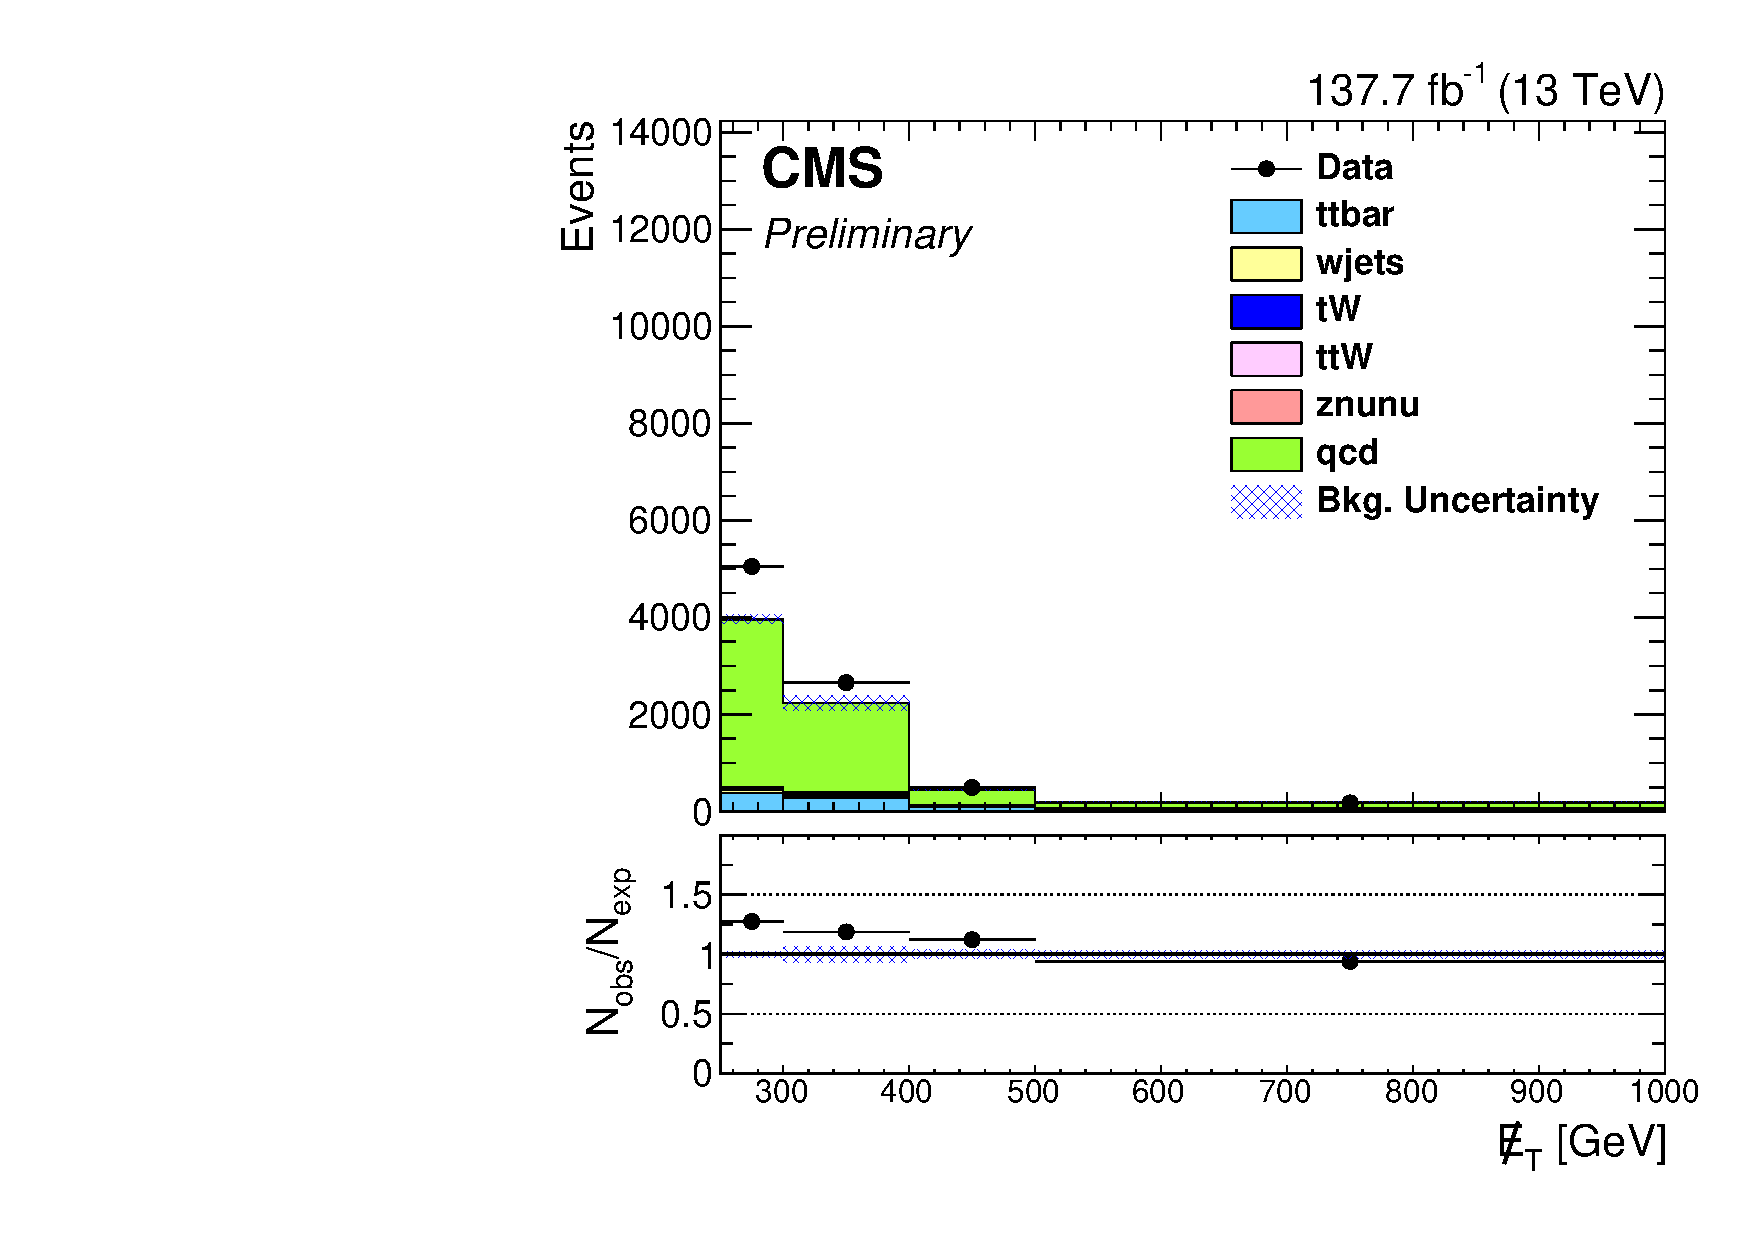
\includegraphics[width=0.32\textwidth]{../Research/SUSY/2019/LLB/lepcr_allEras/MET_pt_DataMC_hm_nb1_lowmtb_nj7_nrtgeq1__.pdf}
  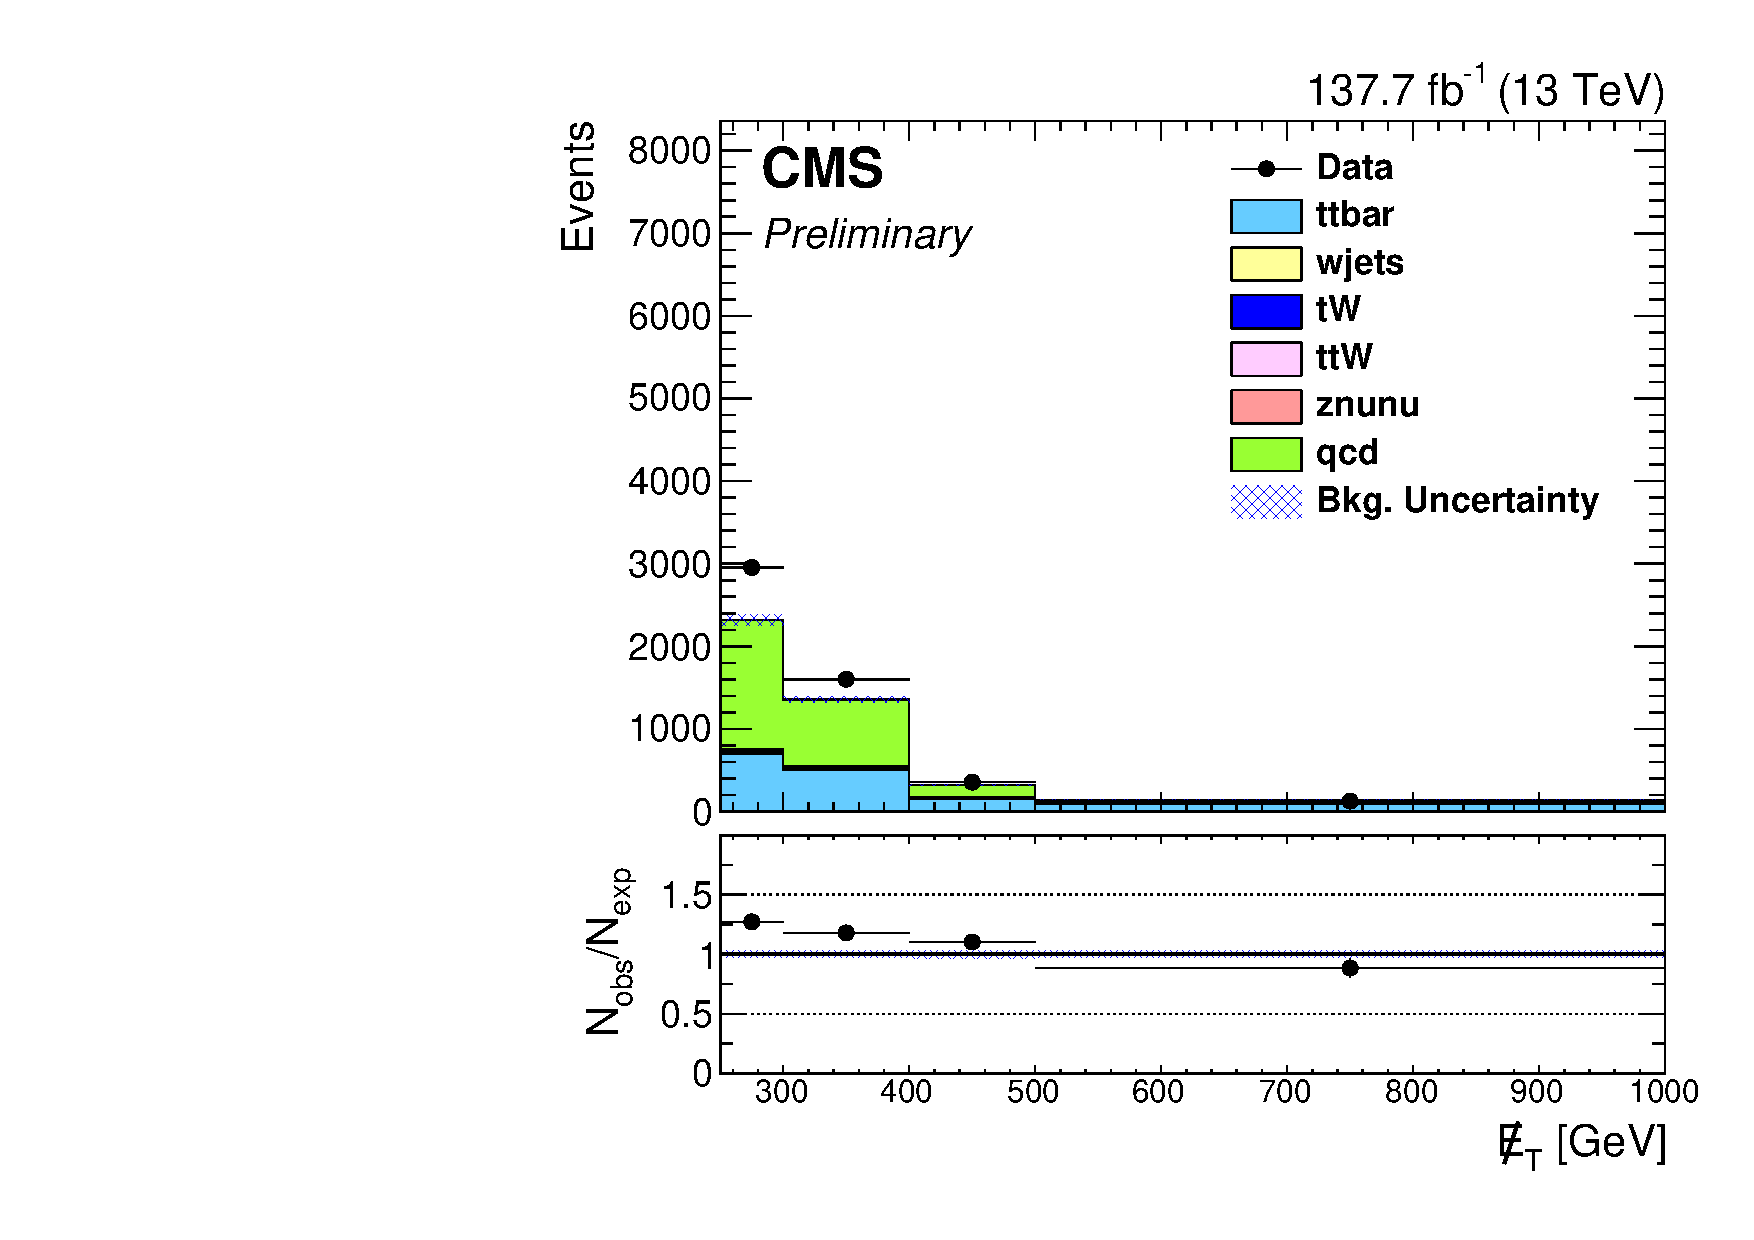
\includegraphics[width=0.32\textwidth]{../Research/SUSY/2019/LLB/lepcr_allEras/MET_pt_DataMC_hm_nb2_lowmtb_nj7_nrtgeq1__.pdf} \\
  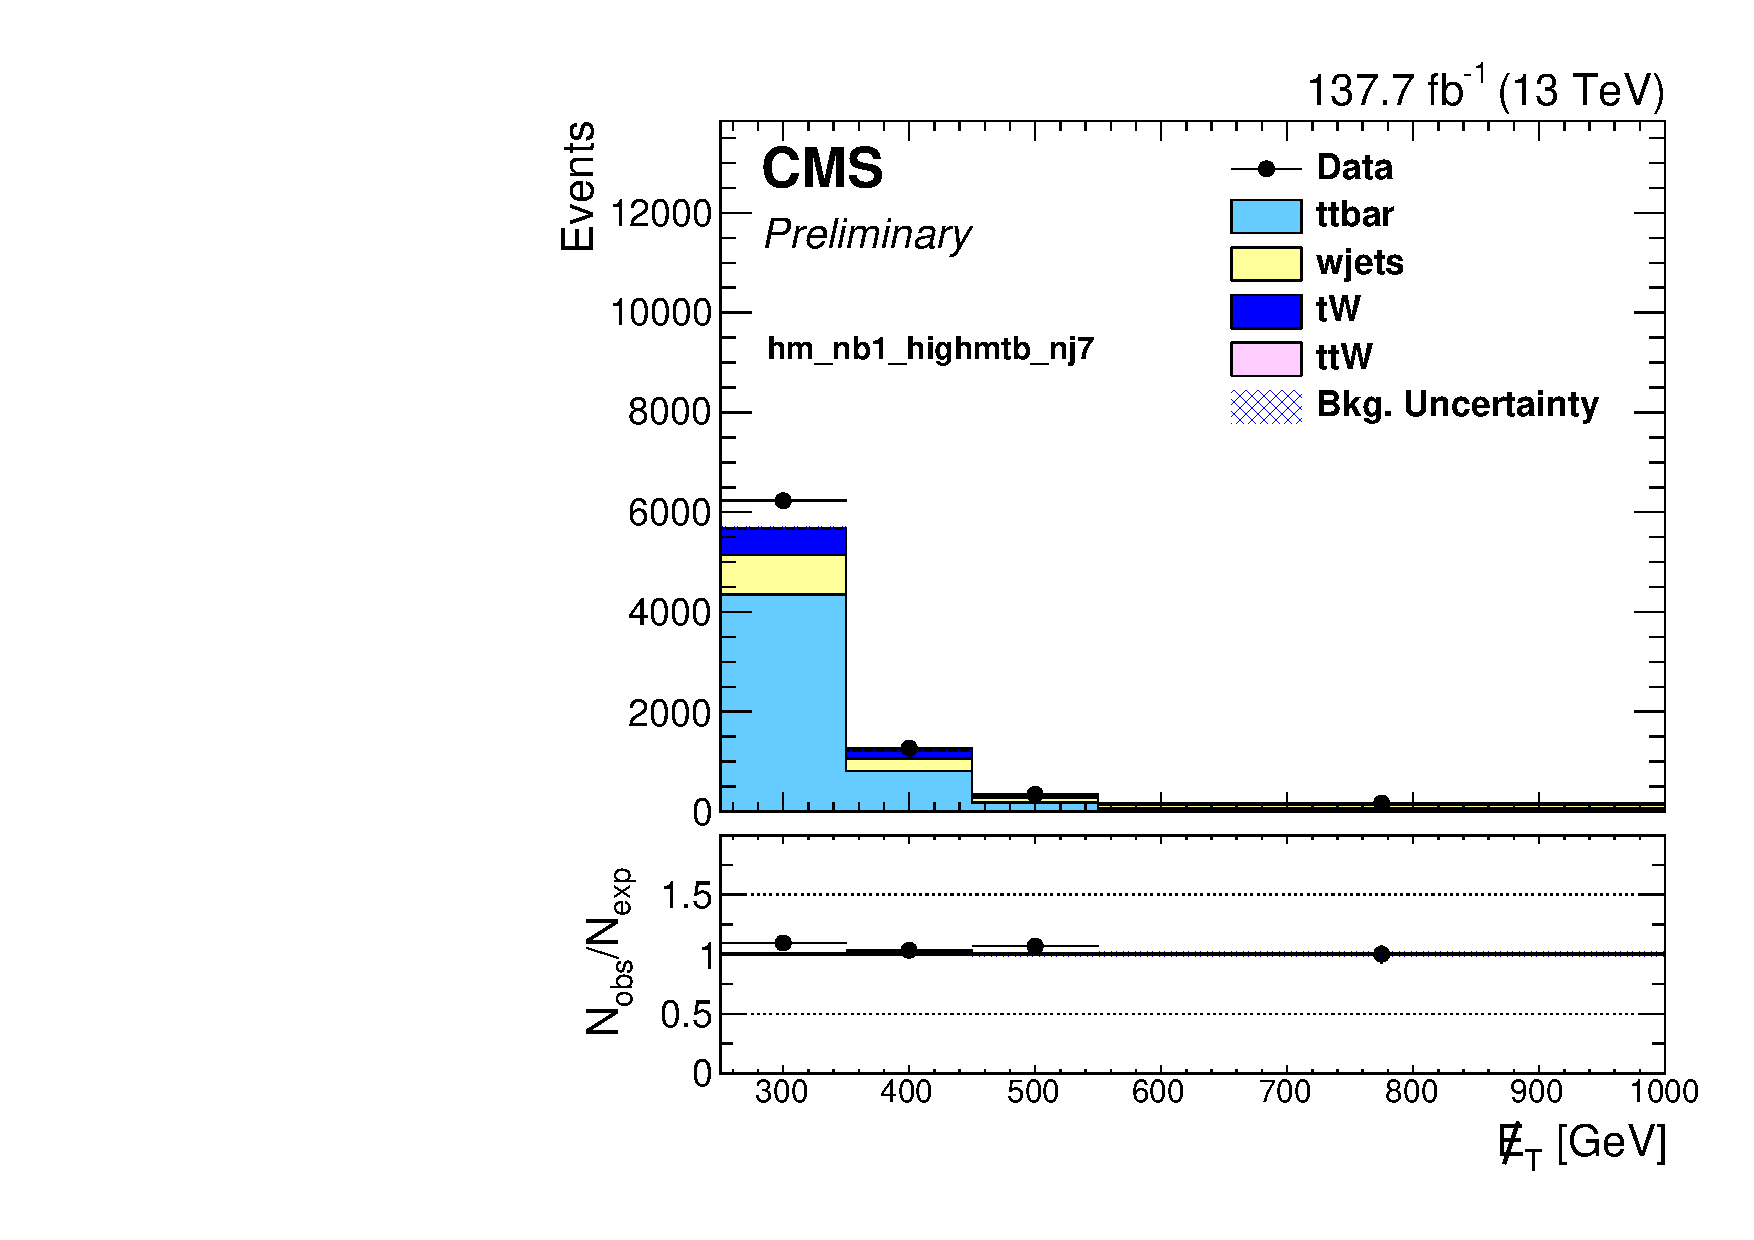
\includegraphics[width=0.32\textwidth]{../Research/SUSY/2019/LLB/lepcr_allEras/MET_pt_DataMC_hm_nb1_highmtb_nj7_nt0_nrt0_nw0__.pdf}
  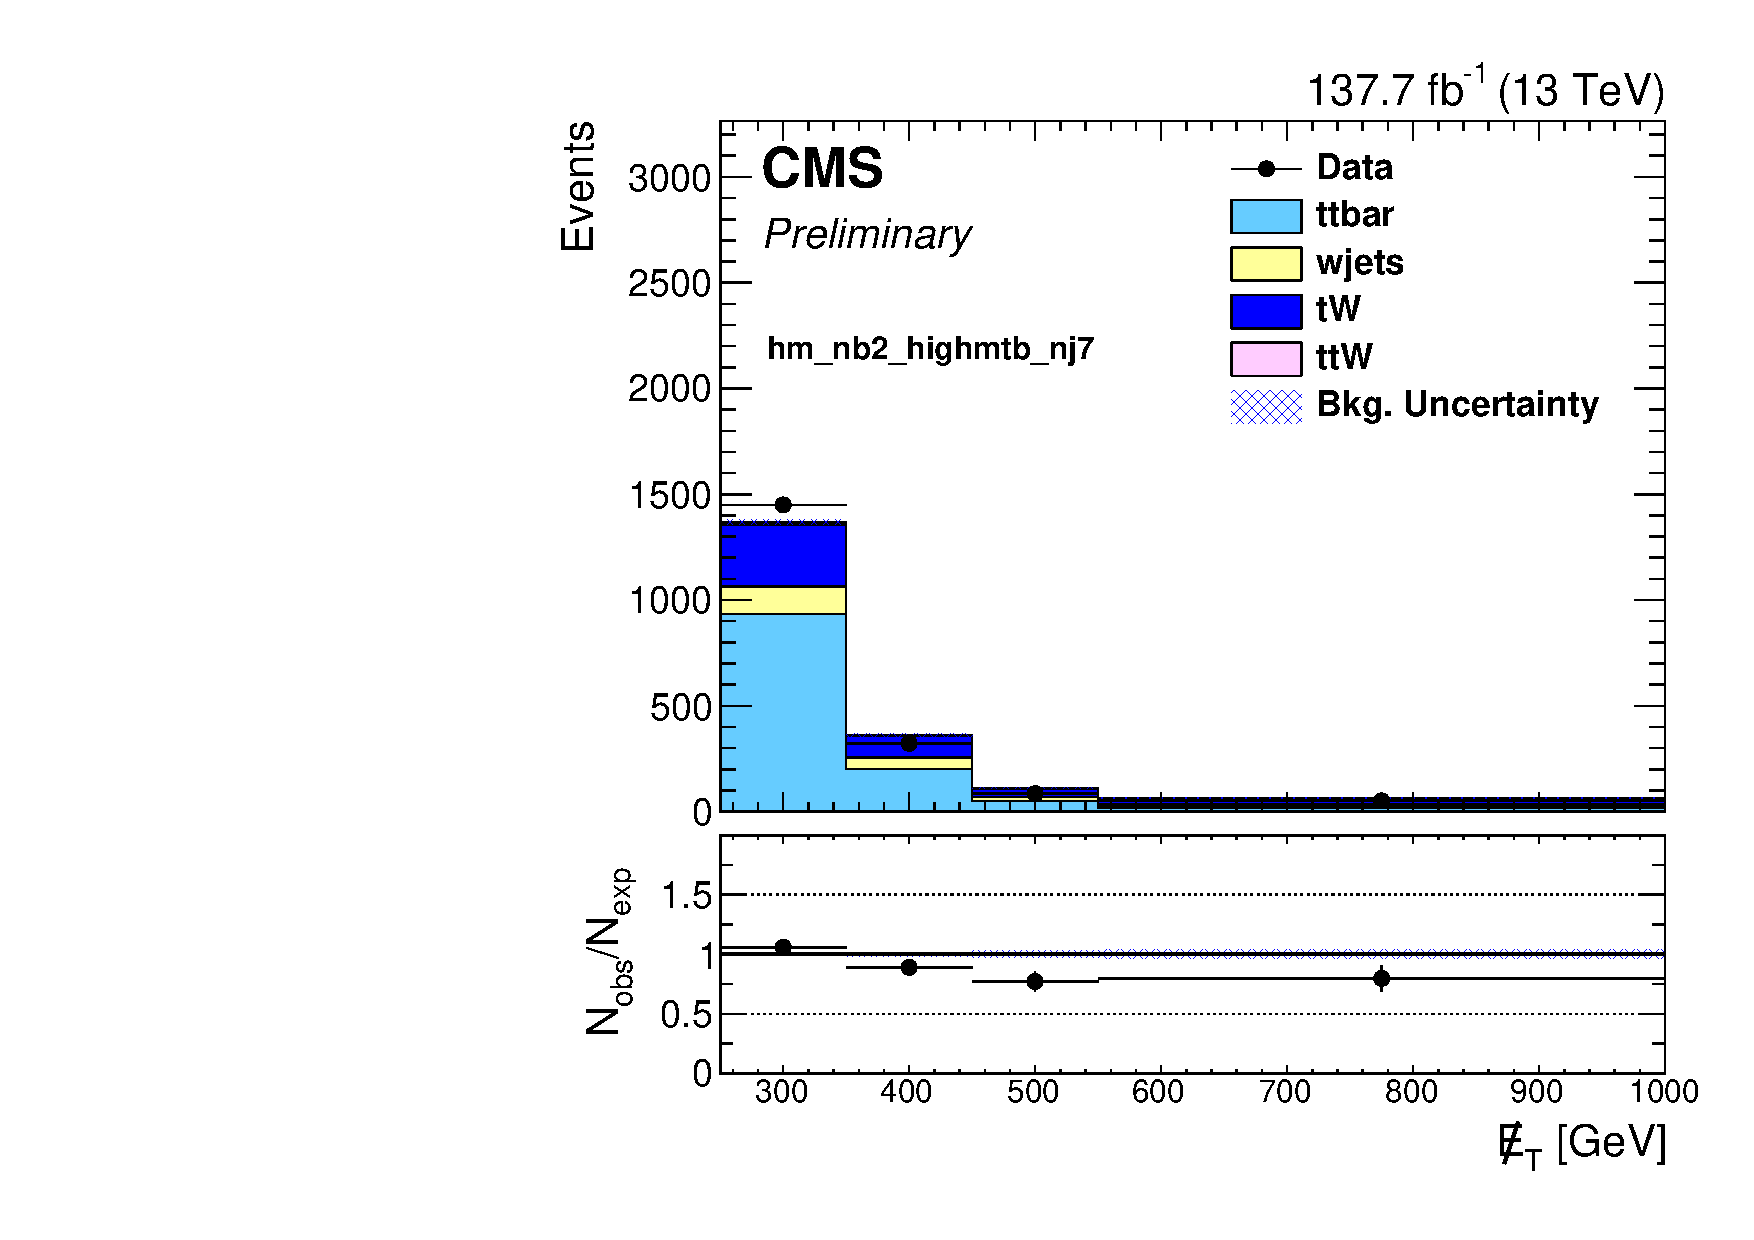
\includegraphics[width=0.32\textwidth]{../Research/SUSY/2019/LLB/lepcr_allEras/MET_pt_DataMC_hm_nb2_highmtb_nj7_nt0_nrt0_nw0__.pdf} \\
	\end{center}
	\caption{Comparison of the \met~distribution in the single-lepton sample after applying the high \dm~baseline selection in the $\mtb<175~\GeV$ and $\nt=0, \nrt=0,$ and $\nw=0$ region. Data and simulation are represented by the black points and stacked histograms, respectively. The error bars on the ratio of observed data to simulation correspond to the data statistical uncertainty and the shaded blue band represents the statistical uncertainty on the simulation. These regions are included with the search regions in the simultaneous fit for the signal extraction in order to estimate the LL contribution.
	 %               The plots in the top row are for events with $\mtb<175$~\GeV, with $5\leq\nj<7$ on the left and $\nj\geq7$ on the right. 
	 %               The plots in the middle row are for events with $\mtb>175$~\GeV and $\nt=0, \nw=0$, with $5\leq\nj<7$ on the left and $\nj\geq7$ on the right. 
	 %               The plot in the bottom row is for events with $\mtb>175$~\GeV and $\nj\geq5$, with $\nt=0, \nw\geq1$ on the left, $\nt\geq1, \nw=0$ on the middle, and $\nt\geq1$, and $\nw\geq1$ on the right.
	 }
	\label{fig:llb-1lcr-datavsmc-hm-nt0-nrt0-nw0}
\end{figure}

\begin{figure}[!htb]
	\begin{center}
  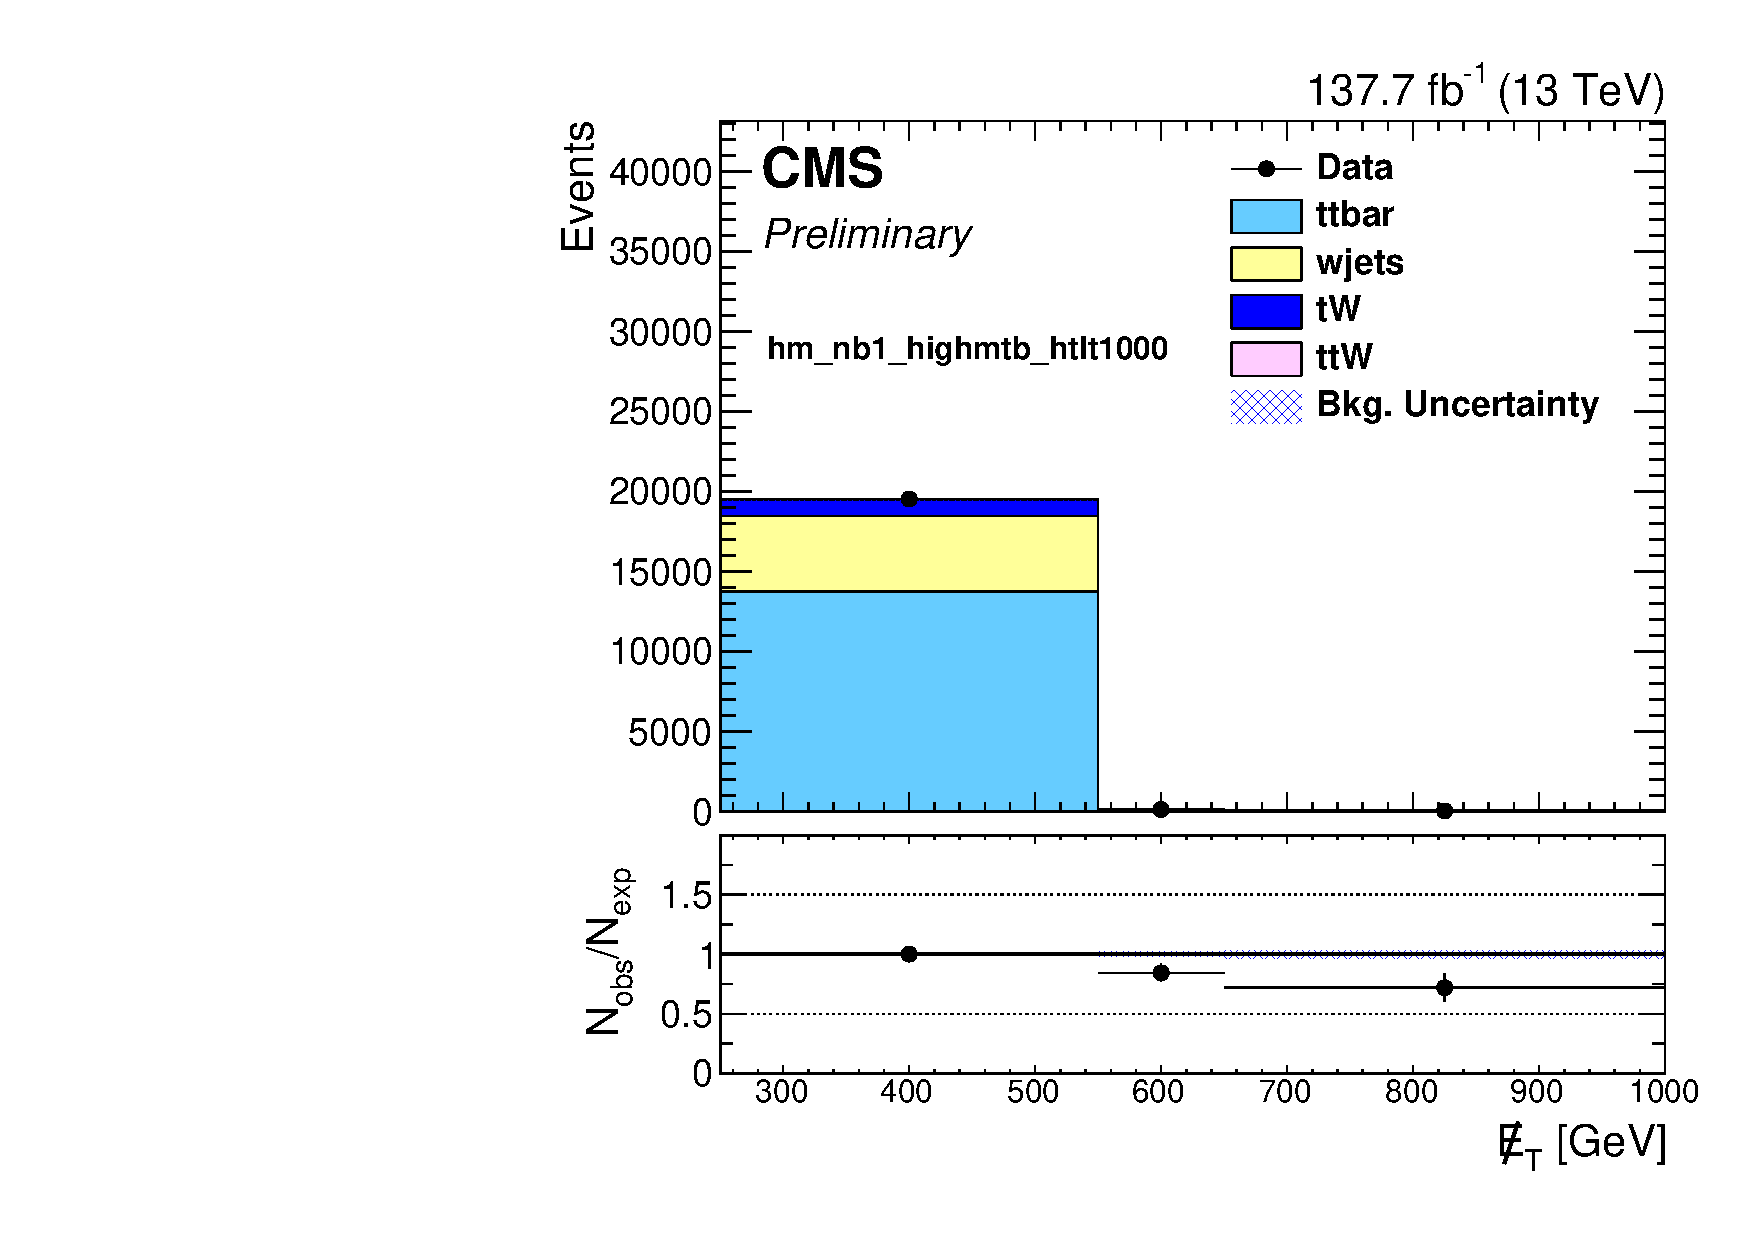
\includegraphics[width=0.32\textwidth]{../Research/SUSY/2019/LLB/lepcr_allEras/MET_pt_DataMC_hm_nb1_highmtb_ntgeq1_nrt0_nw0_htlt1000__.pdf}
  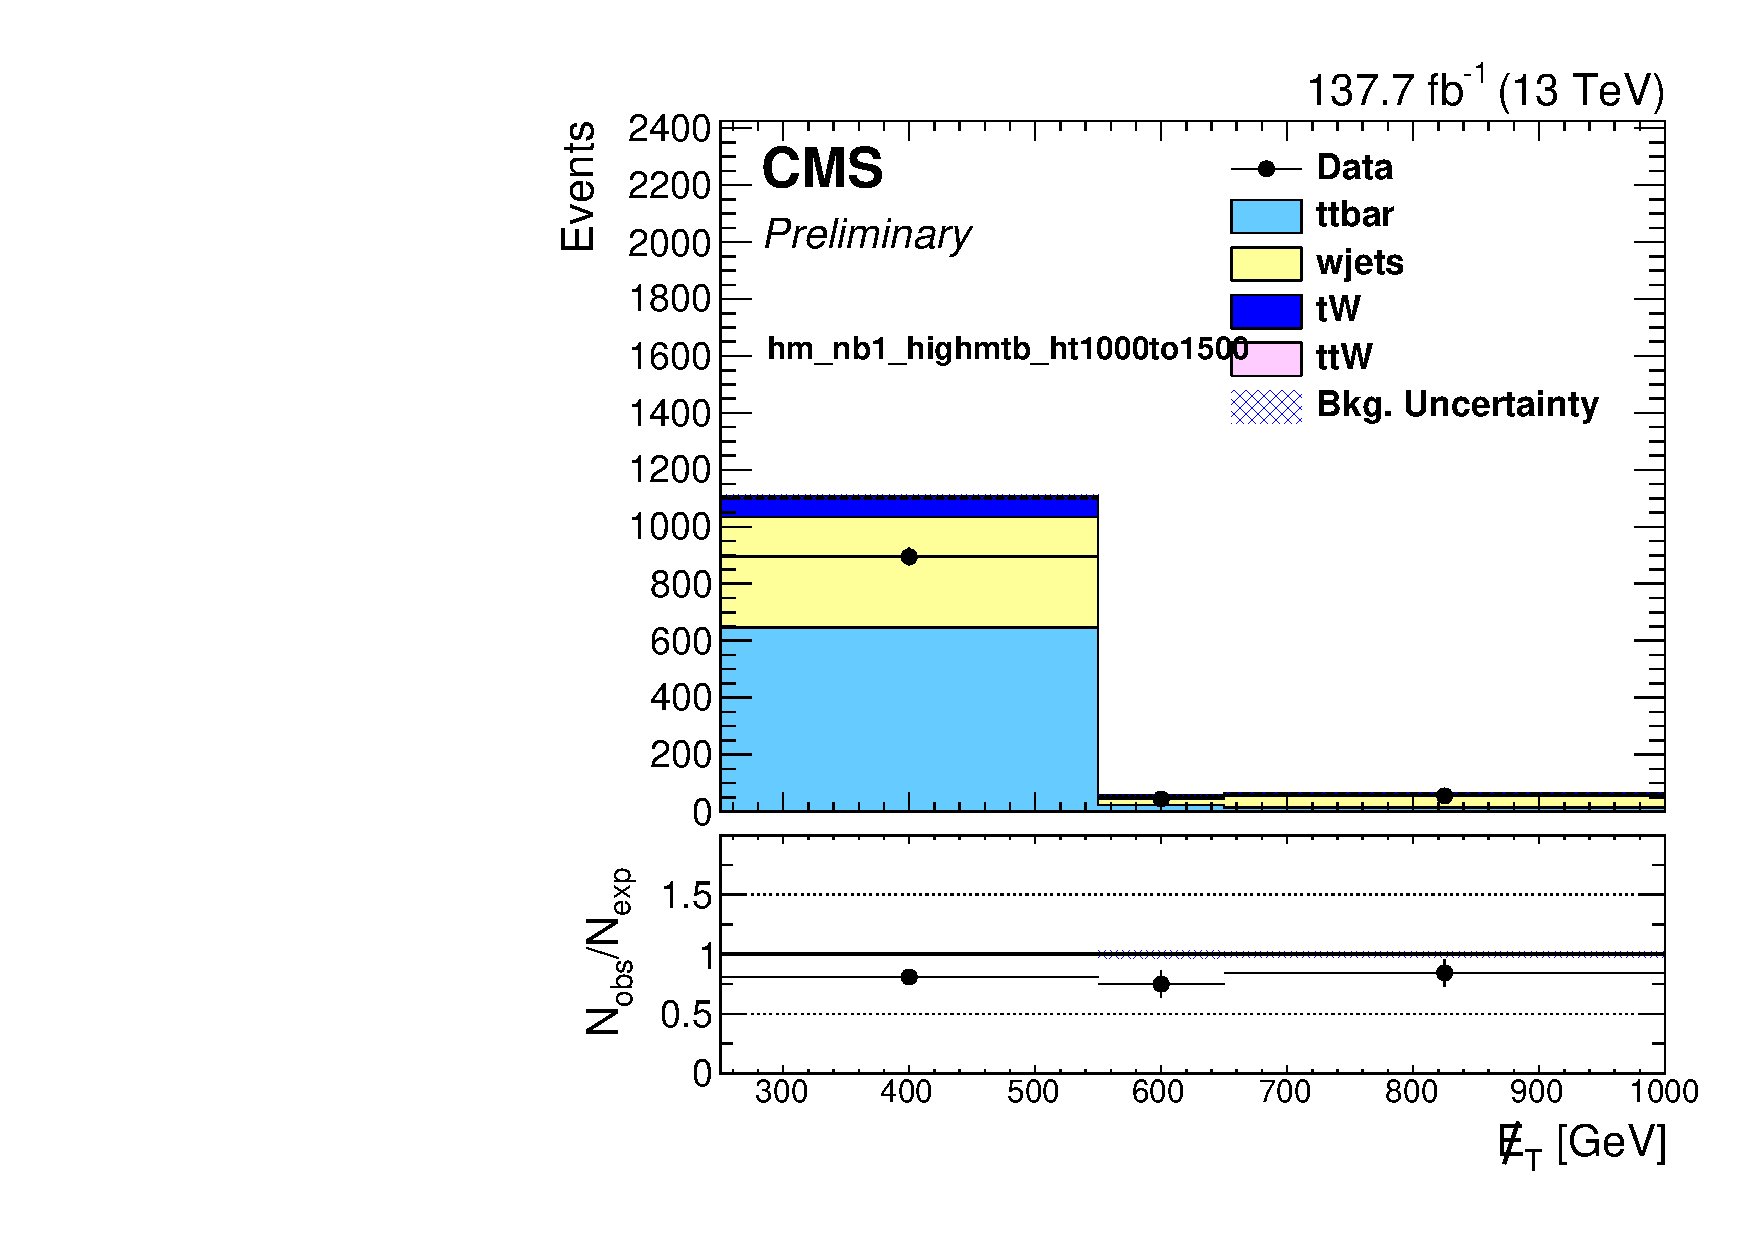
\includegraphics[width=0.32\textwidth]{../Research/SUSY/2019/LLB/lepcr_allEras/MET_pt_DataMC_hm_nb1_highmtb_ntgeq1_nrt0_nw0_ht1000to1500__.pdf}
  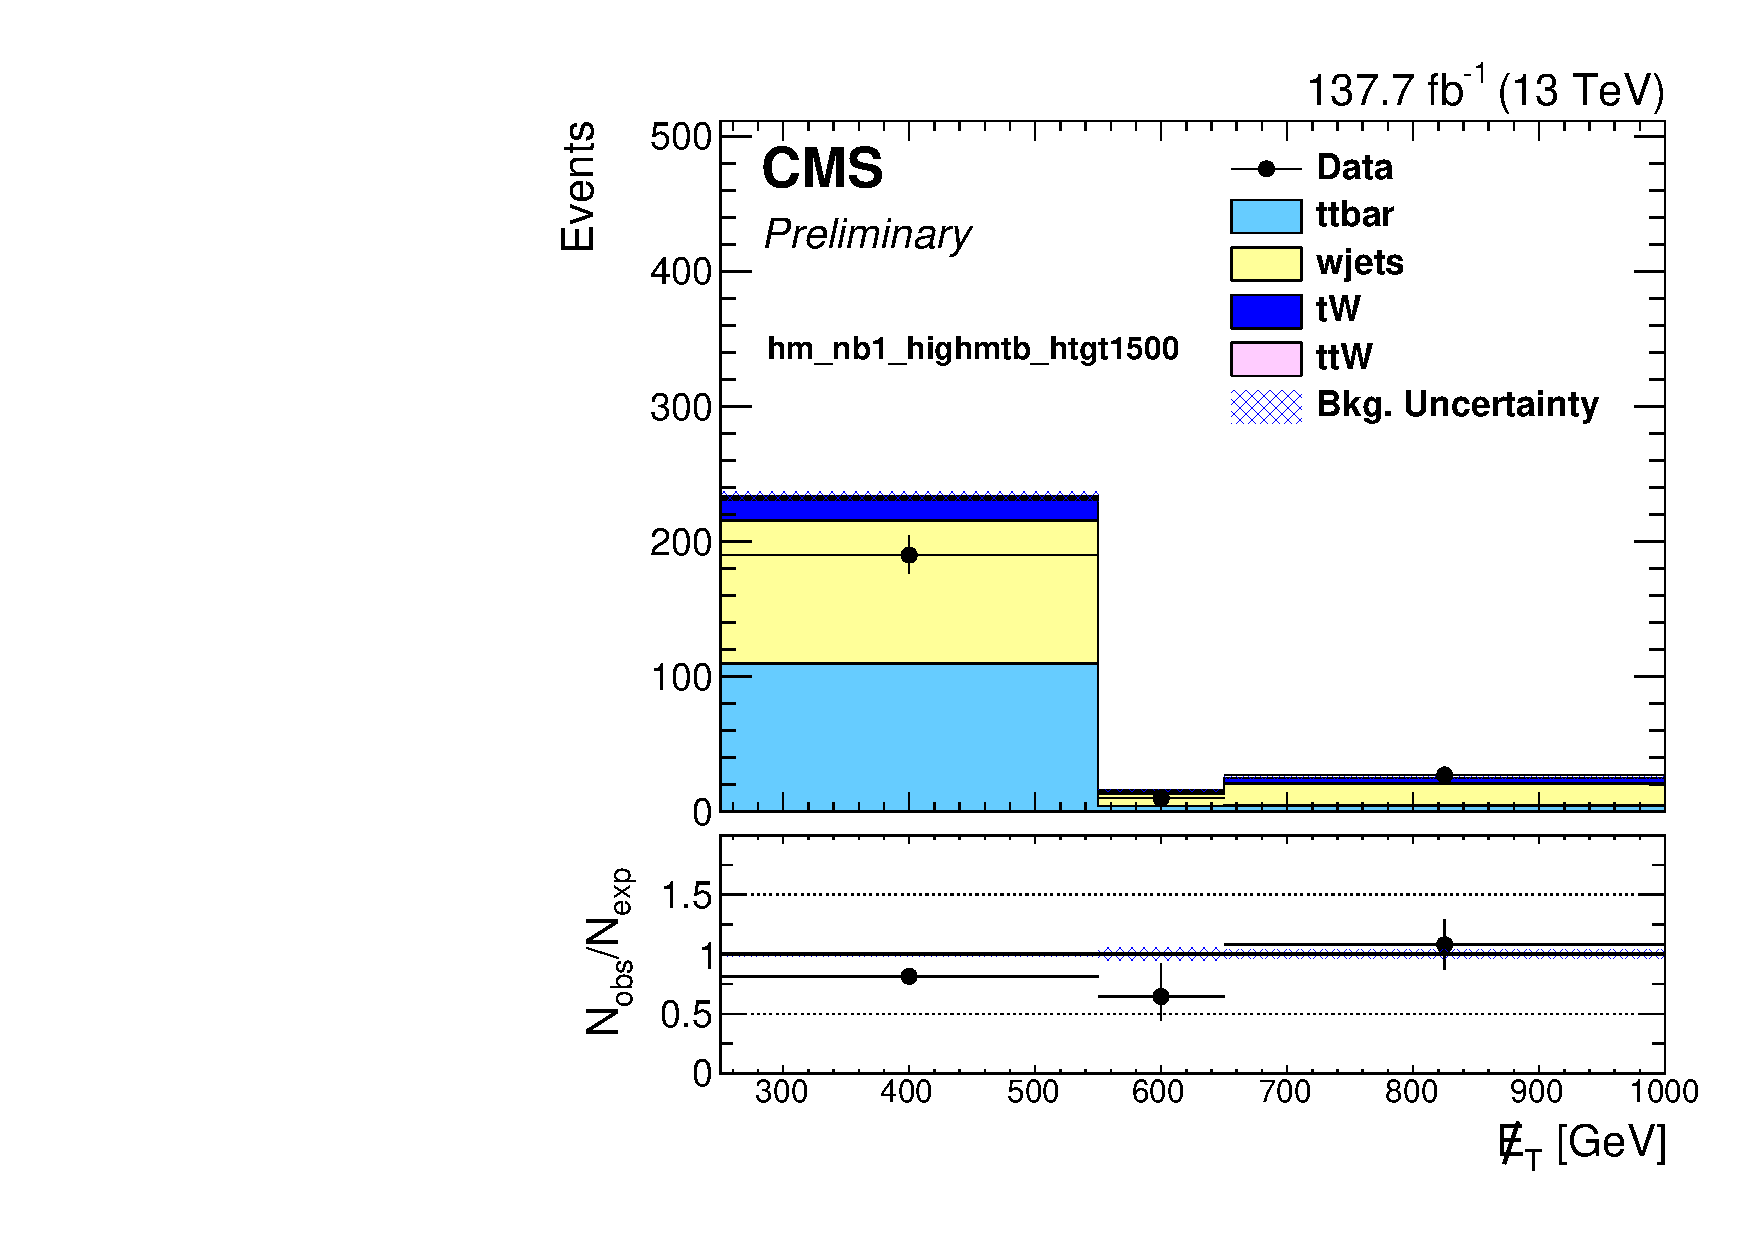
\includegraphics[width=0.32\textwidth]{../Research/SUSY/2019/LLB/lepcr_allEras/MET_pt_DataMC_hm_nb1_highmtb_ntgeq1_nrt0_nw0_htgt1500__.pdf} \\
  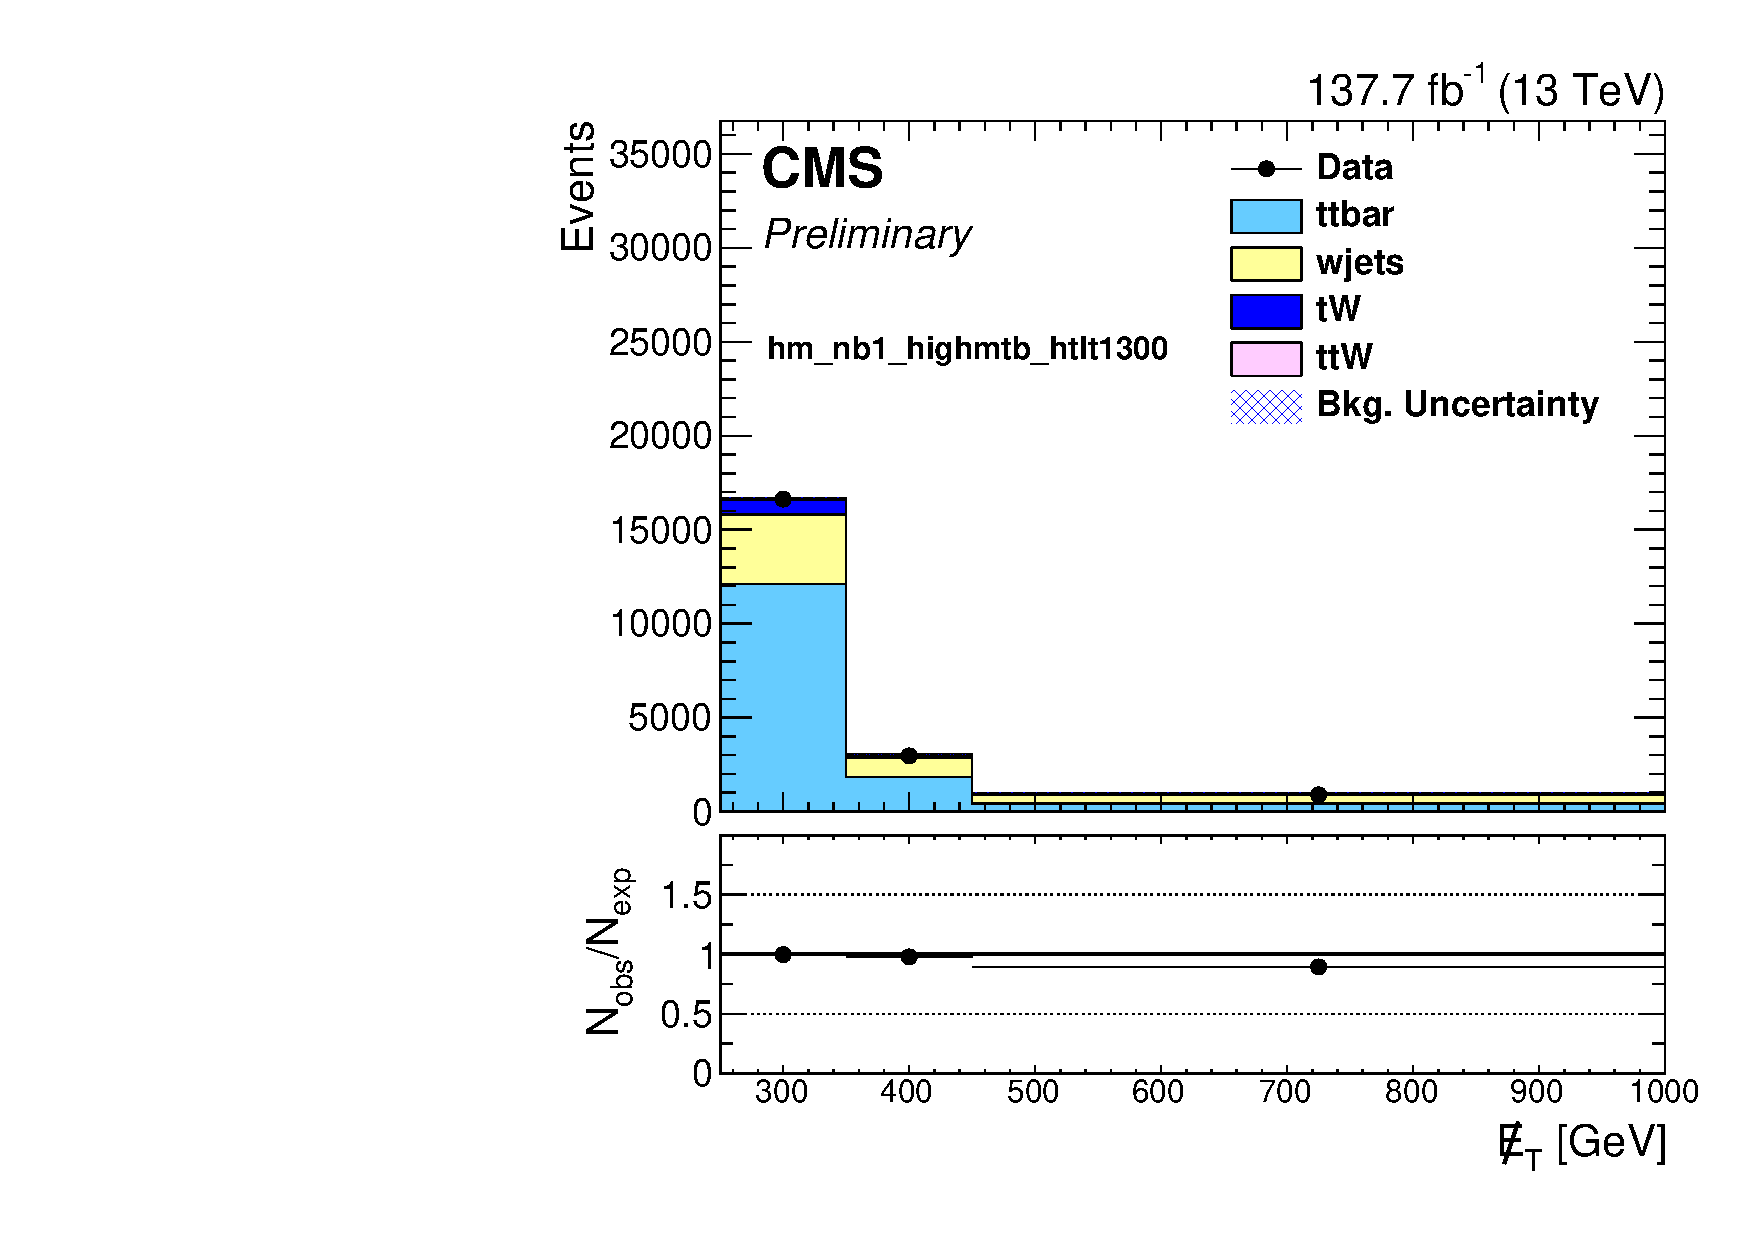
\includegraphics[width=0.32\textwidth]{../Research/SUSY/2019/LLB/lepcr_allEras/MET_pt_DataMC_hm_nb1_highmtb_nt0_nrt0_nwgeq1_htlt1300__.pdf} 
  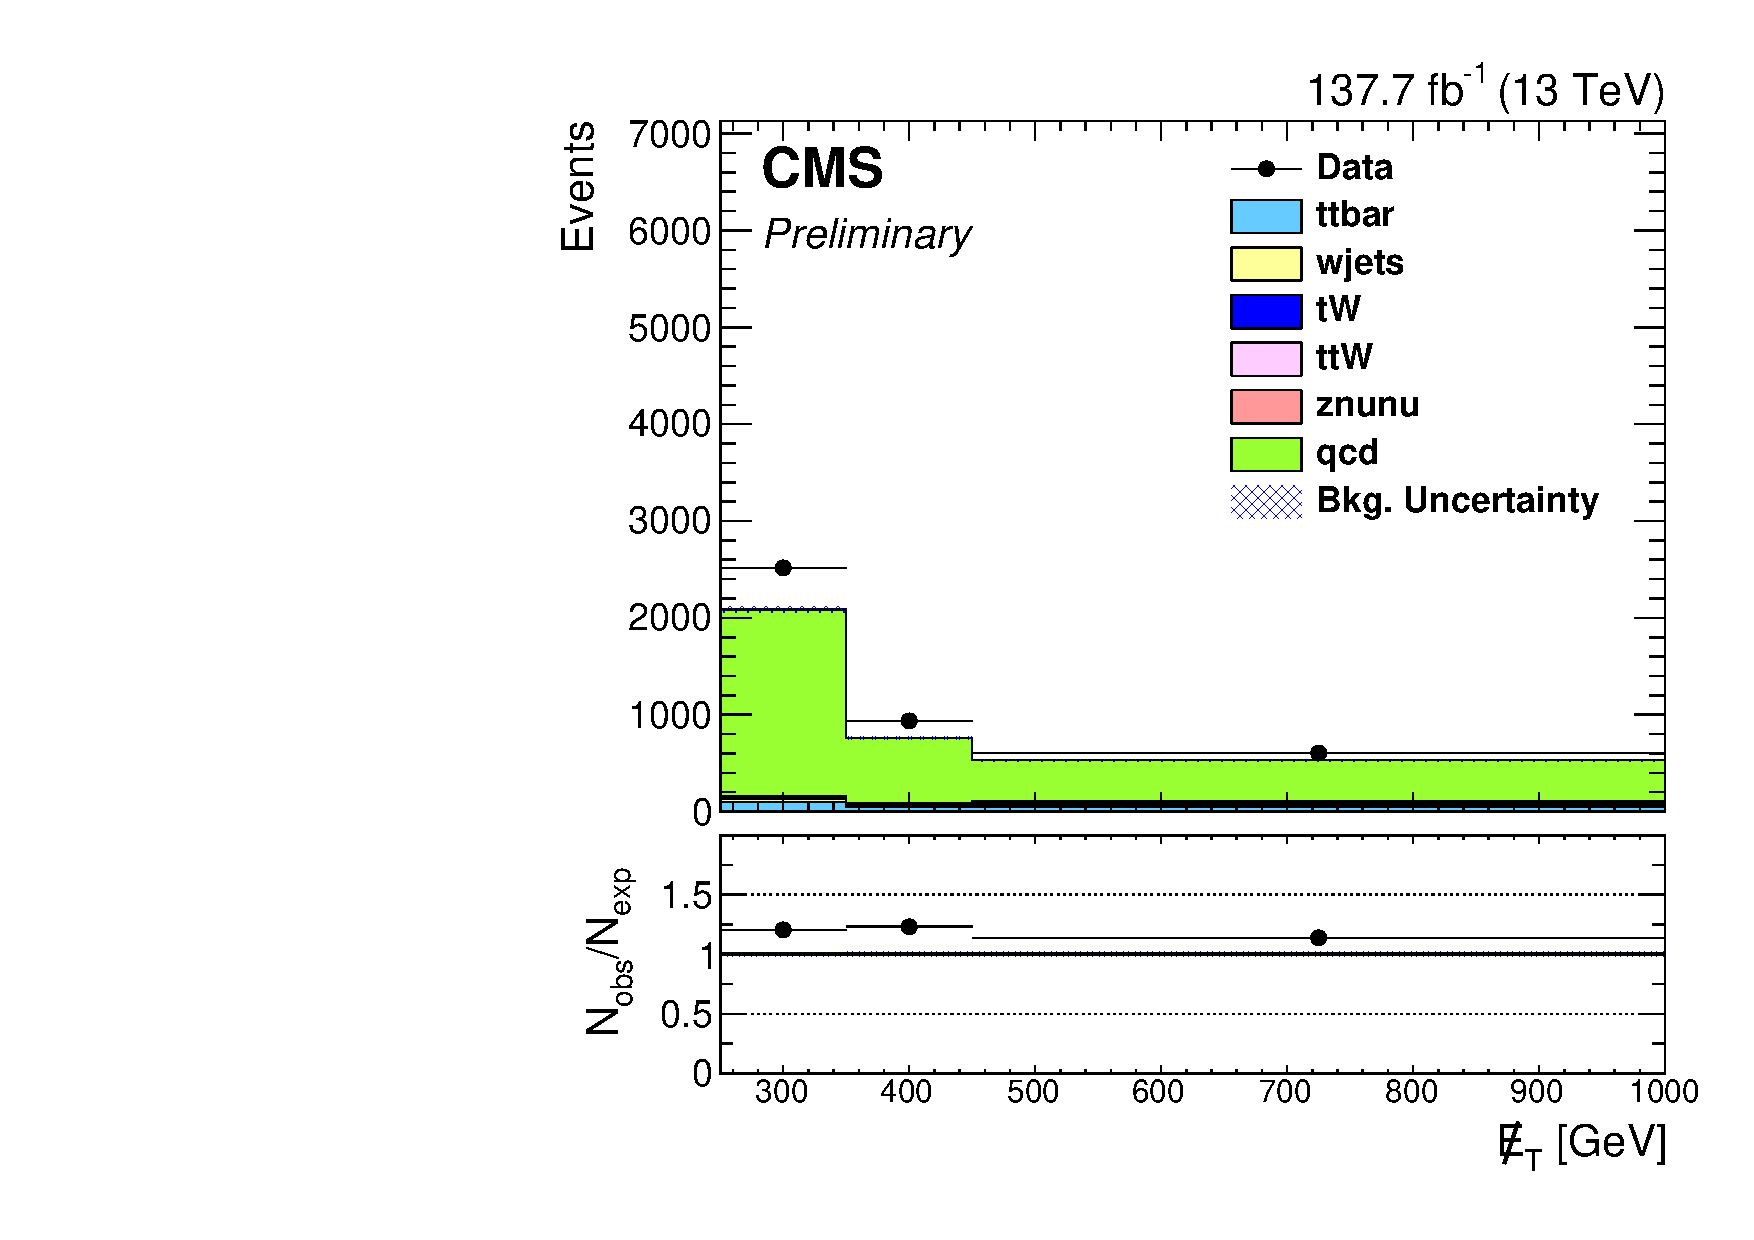
\includegraphics[width=0.32\textwidth]{../Research/SUSY/2019/LLB/lepcr_allEras/MET_pt_DataMC_hm_nb1_highmtb_nt0_nrt0_nwgeq1_htgt1300__.pdf} \\
  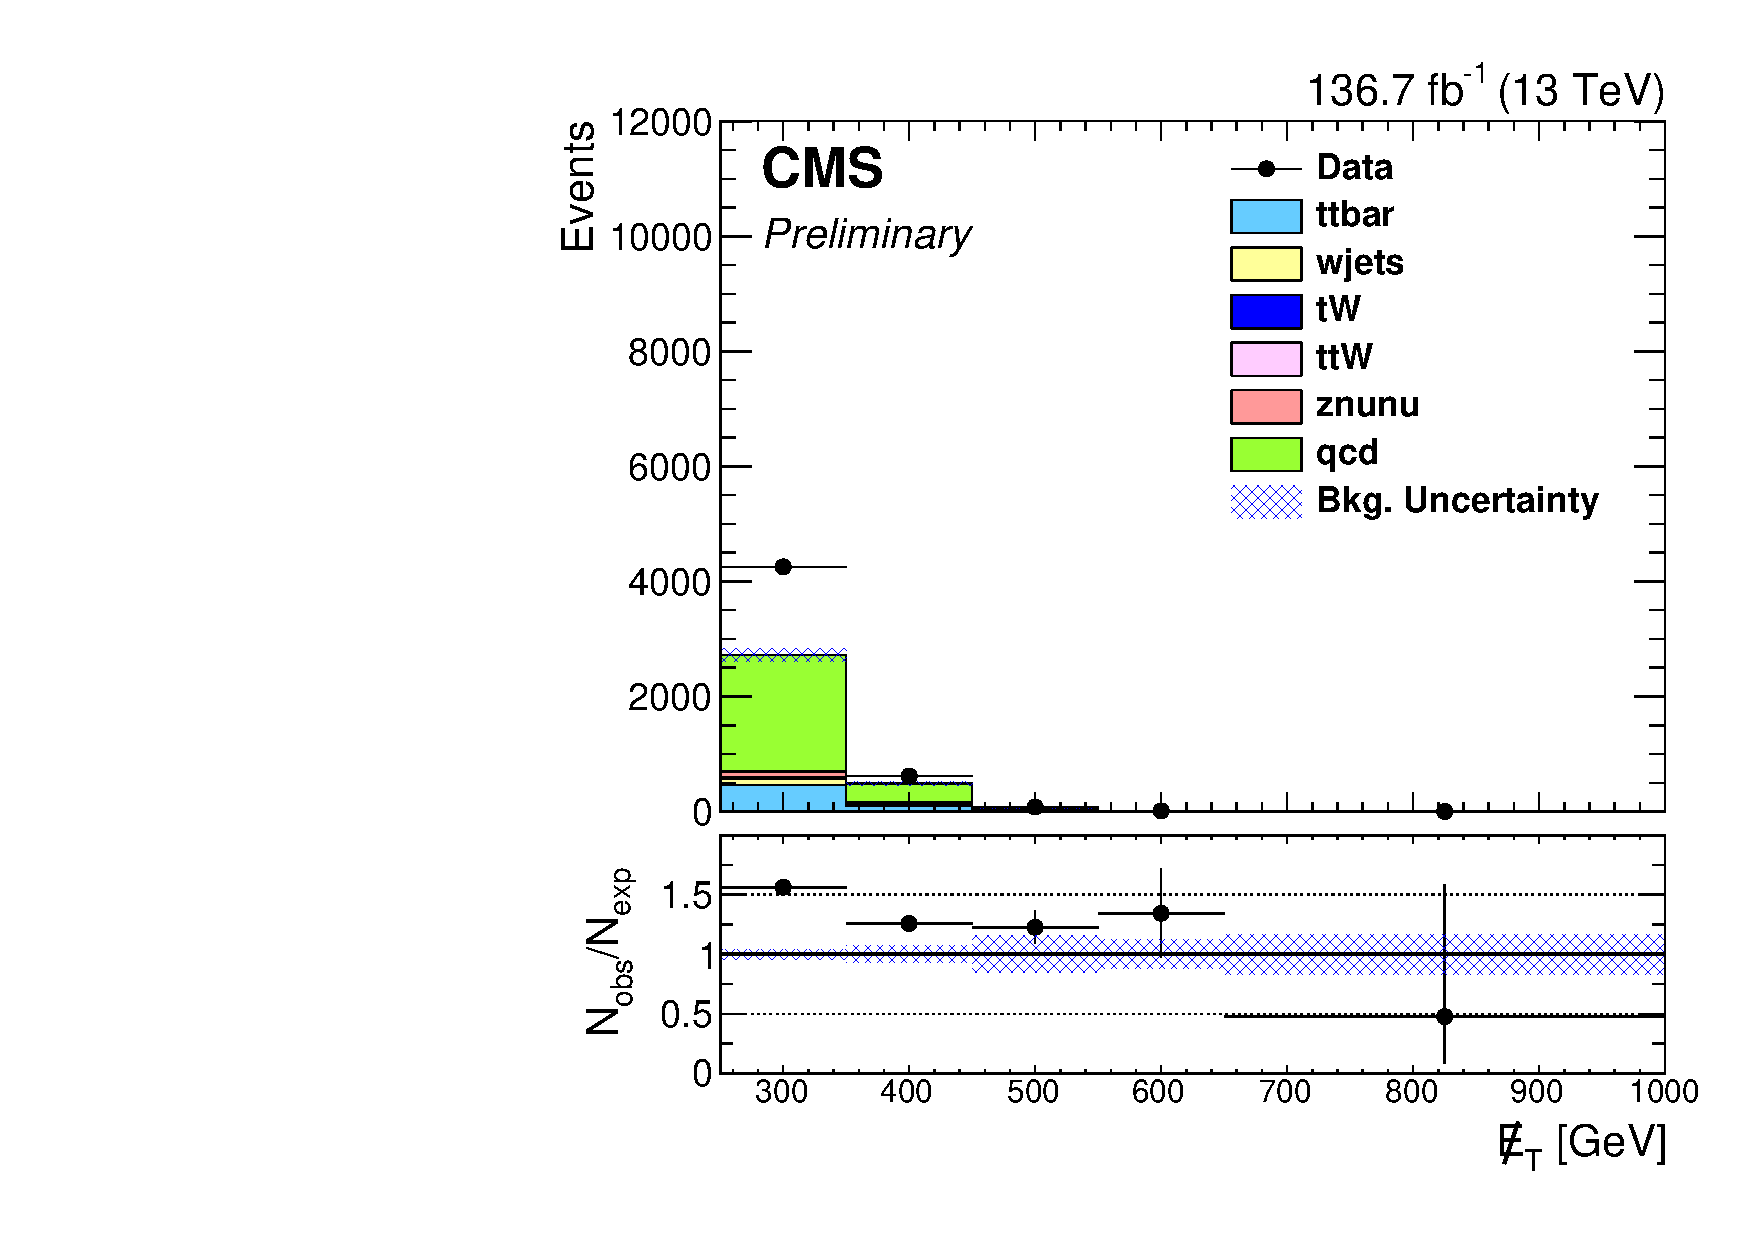
\includegraphics[width=0.32\textwidth]{../Research/SUSY/2019/LLB/lepcr_allEras/MET_pt_DataMC_hm_nb1_highmtb_nt0_nrtgeq1_nw0_htlt1000__.pdf} 
  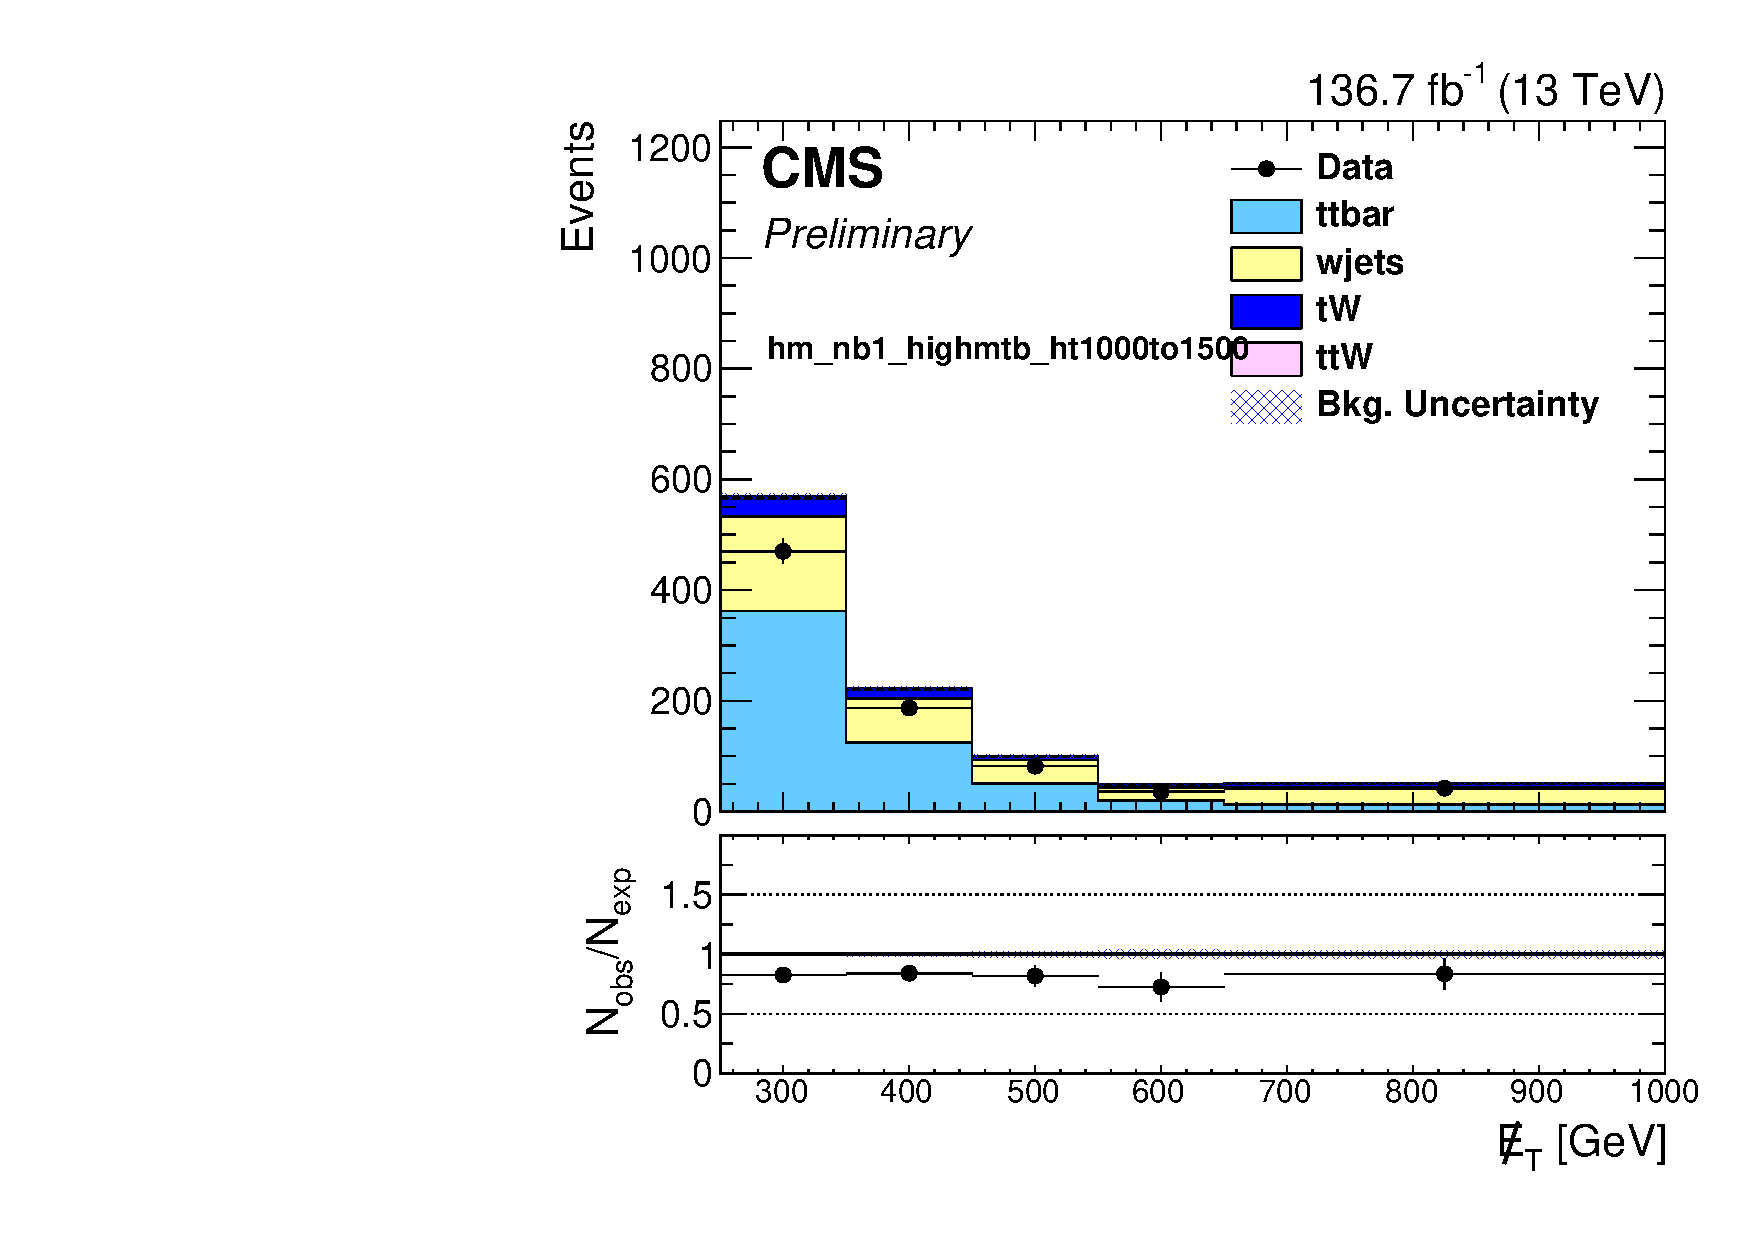
\includegraphics[width=0.32\textwidth]{../Research/SUSY/2019/LLB/lepcr_allEras/MET_pt_DataMC_hm_nb1_highmtb_nt0_nrtgeq1_nw0_ht1000to1500__.pdf} 
  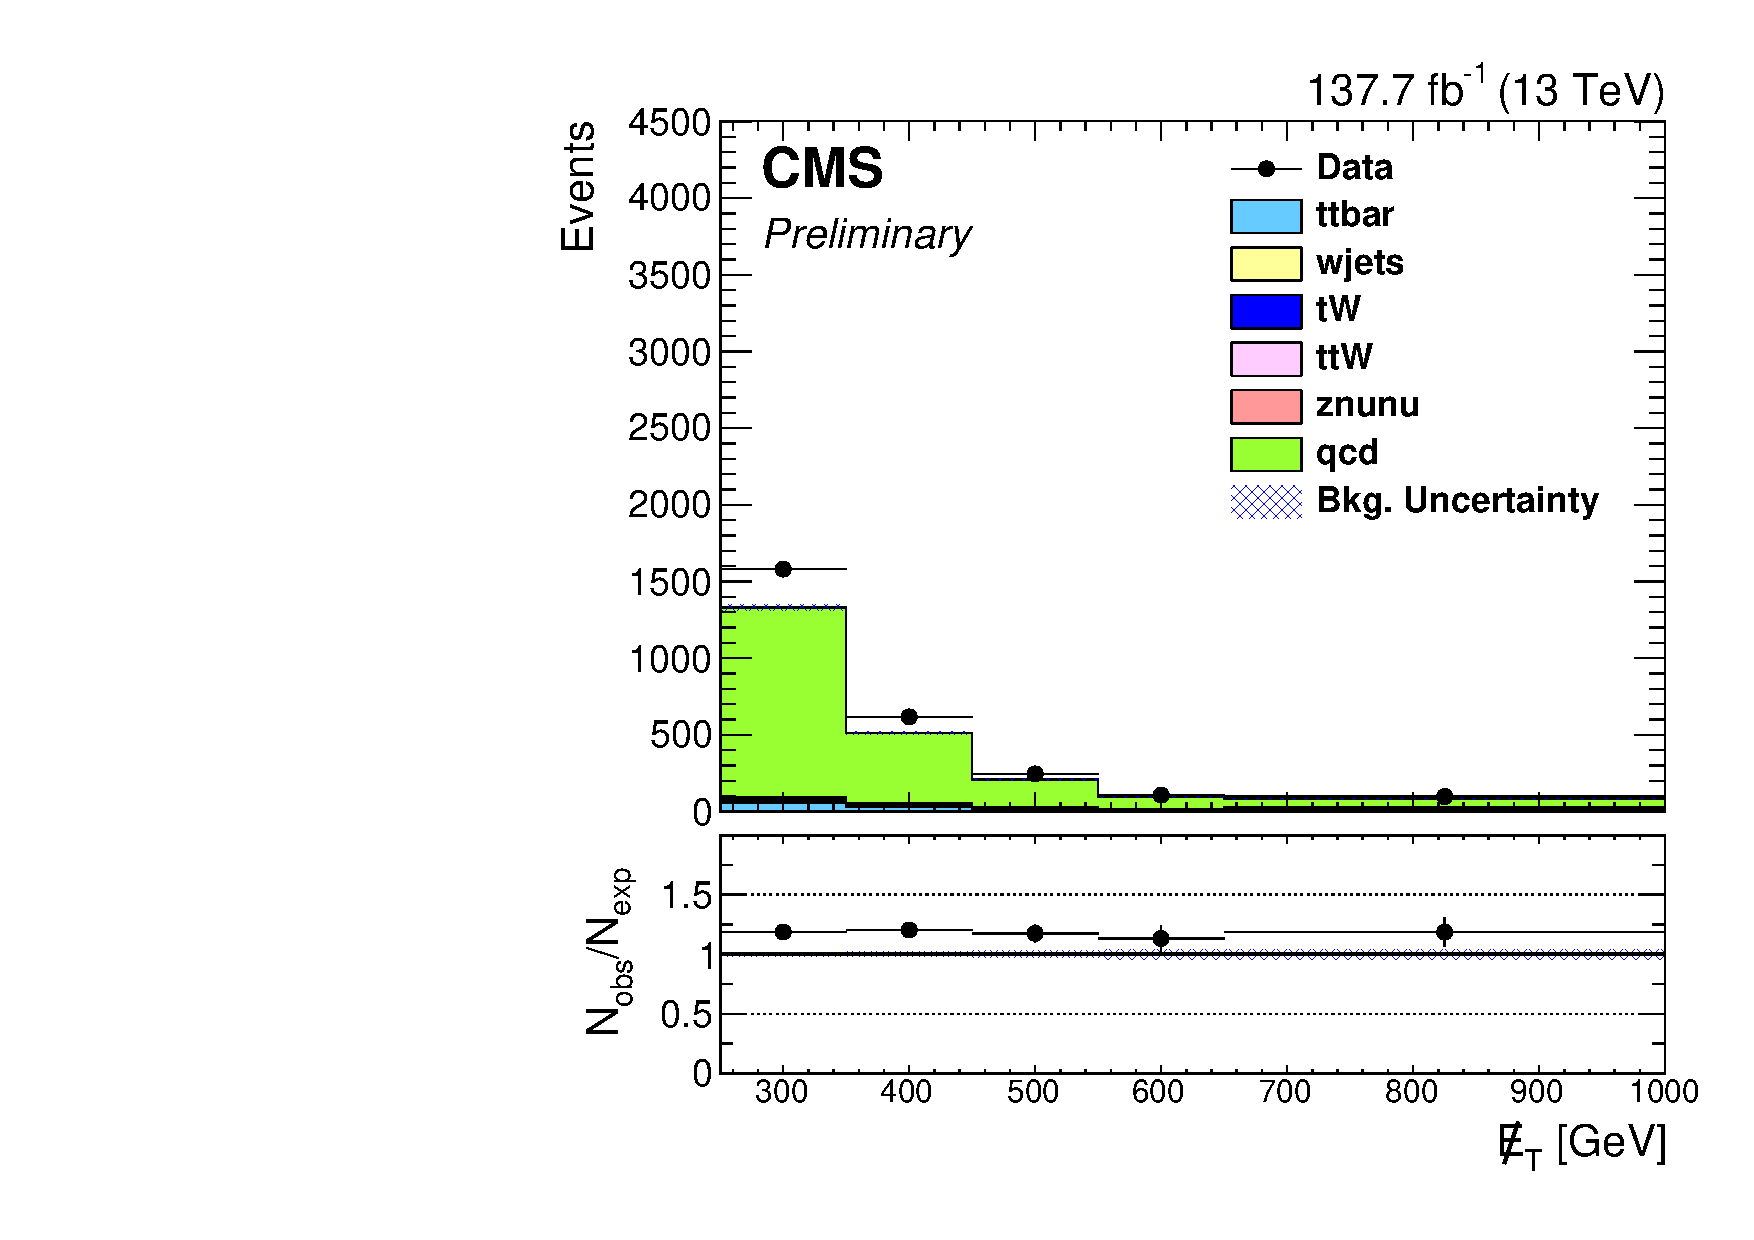
\includegraphics[width=0.32\textwidth]{../Research/SUSY/2019/LLB/lepcr_allEras/MET_pt_DataMC_hm_nb1_highmtb_nt0_nrtgeq1_nw0_htgt1500__.pdf} \\
  \includegraphics[width=0.32\textwidth]{../Research/SUSY/2019/LLB/lepcr_allEras/MET_pt_DataMC_hm_nb1_highmtb_ntgeq1_nrt0_nwgeq1__.pdf} 
  \includegraphics[width=0.32\textwidth]{../Research/SUSY/2019/LLB/lepcr_allEras/MET_pt_DataMC_hm_nb1_highmtb_ntgeq1_nrtgeq1_nw0__.pdf} 
  \includegraphics[width=0.32\textwidth]{../Research/SUSY/2019/LLB/lepcr_allEras/MET_pt_DataMC_hm_nb1_highmtb_nt0_nrtgeq1_nwgeq1__.pdf} \\
	\end{center}
	\caption{Comparison of the \met~distribution in the single-lepton sample after applying the high \dm~baseline selection in the $\nb=1$ region where there are $\geq1$ heavy object tags. Data and simulation are represented by the black points and stacked histograms, respectively. The error bars on the ratio of observed data to simulation correspo    nd to the data statistical uncertainty and the shaded blue band represents the statistical uncertainty on the simulation. These regions are included with the search regions in the simultaneous fit for the signal extraction in order to estimate the LL contribution.
	 %               The plots in the top row are for events with $\mtb<175$~\GeV, with $5\leq\nj<7$ on the left and $\nj\geq7$ on the right. 
	 %               The plots in the middle row are for events with $\mtb>175$~\GeV and $\nt=0, \nw=0$, with $5\leq\nj<7$ on the left and $\nj\geq7$ on the right. 
	 %               The plot in the bottom row is for events with $\mtb>175$~\GeV and $\nj\geq5$, with $\nt=0, \nw\geq1$ on the left, $\nt\geq1, \nw=0$ on the middle, and $\nt\geq1$, and $\nw\geq1$ on the right.
	 }
	\label{fig:llb-1lcr-datavsmc-hm-nb1}
\end{figure}

\begin{figure}[!htb]
	\begin{center}
  \includegraphics[width=0.32\textwidth]{../Research/SUSY/2019/LLB/lepcr_allEras/MET_pt_DataMC_hm_nbeq2_highmtb_nt1_nrt0_nw0_htlt1000__.pdf}
  \includegraphics[width=0.32\textwidth]{../Research/SUSY/2019/LLB/lepcr_allEras/MET_pt_DataMC_hm_nbeq2_highmtb_nt1_nrt0_nw0_ht1000to1500__.pdf}
  \includegraphics[width=0.32\textwidth]{../Research/SUSY/2019/LLB/lepcr_allEras/MET_pt_DataMC_hm_nbeq2_highmtb_nt1_nrt0_nw0_htgt1500__.pdf} \\
  \includegraphics[width=0.32\textwidth]{../Research/SUSY/2019/LLB/lepcr_allEras/MET_pt_DataMC_hm_nbeq2_highmtb_nt0_nrt0_nw1_htlt1300__.pdf} 
  \includegraphics[width=0.32\textwidth]{../Research/SUSY/2019/LLB/lepcr_allEras/MET_pt_DataMC_hm_nbeq2_highmtb_nt0_nrt0_nw1_htgt1300__.pdf} \\
  \includegraphics[width=0.32\textwidth]{../Research/SUSY/2019/LLB/lepcr_allEras/MET_pt_DataMC_hm_nbeq2_highmtb_nt0_nrt1_nw0_htlt1000__.pdf} 
  \includegraphics[width=0.32\textwidth]{../Research/SUSY/2019/LLB/lepcr_allEras/MET_pt_DataMC_hm_nbeq2_highmtb_nt0_nrt1_nw0_ht1000to1500__.pdf} 
  \includegraphics[width=0.32\textwidth]{../Research/SUSY/2019/LLB/lepcr_allEras/MET_pt_DataMC_hm_nbeq2_highmtb_nt0_nrt1_nw0_htgt1500__.pdf} \\
  \includegraphics[width=0.32\textwidth]{../Research/SUSY/2019/LLB/lepcr_allEras/MET_pt_DataMC_hm_nbeq2_highmtb_nt1_nrt0_nw1__.pdf} 
  \includegraphics[width=0.32\textwidth]{../Research/SUSY/2019/LLB/lepcr_allEras/MET_pt_DataMC_hm_nbeq2_highmtb_nt0_nrt1_nw1__.pdf} \\
	\end{center}
	\caption{Comparison of the \met~distribution in the single-lepton sample after applying the high \dm~baseline selection in the $\nb=2$ and $\nt=1, \nrt=1,$ or $\nw=1$ regions. Data and simulation are represented by the black points and stacked histograms, respectively. The error bars on the ratio of observed data to simulation correspo    nd to the data statistical uncertainty and the shaded blue band represents the statistical uncertainty on the simulation. These regions are included with the search regions in the simultaneous fit for the signal extraction in order to estimate the LL contribution.
	 %               The plots in the top row are for events with $\mtb<175$~\GeV, with $5\leq\nj<7$ on the left and $\nj\geq7$ on the right. 
	 %               The plots in the middle row are for events with $\mtb>175$~\GeV and $\nt=0, \nw=0$, with $5\leq\nj<7$ on the left and $\nj\geq7$ on the right. 
	 %               The plot in the bottom row is for events with $\mtb>175$~\GeV and $\nj\geq5$, with $\nt=0, \nw\geq1$ on the left, $\nt\geq1, \nw=0$ on the middle, and $\nt\geq1$, and $\nw\geq1$ on the right.
	 }
	\label{fig:llb-1lcr-datavsmc-hm-nb2-1}
\end{figure}

\begin{figure}[!htb]
	\begin{center}
  \includegraphics[width=0.32\textwidth]{../Research/SUSY/2019/LLB/lepcr_allEras/MET_pt_DataMC_hm_nbeq2_highmtb_nt1_nrt1_nw0_htlt1300__.pdf}
  \includegraphics[width=0.32\textwidth]{../Research/SUSY/2019/LLB/lepcr_allEras/MET_pt_DataMC_hm_nbeq2_highmtb_nt1_nrt1_nw0_htgt1300__.pdf} \\
  \includegraphics[width=0.32\textwidth]{../Research/SUSY/2019/LLB/lepcr_allEras/MET_pt_DataMC_hm_nbeq2_highmtb_nt2_nrt0_nw0_htlt1300__.pdf}
  \includegraphics[width=0.32\textwidth]{../Research/SUSY/2019/LLB/lepcr_allEras/MET_pt_DataMC_hm_nbeq2_highmtb_nt2_nrt0_nw0_htgt1300__.pdf} 
  \includegraphics[width=0.32\textwidth]{../Research/SUSY/2019/LLB/lepcr_allEras/MET_pt_DataMC_hm_nbeq2_highmtb_nt0_nrt0_nw2__.pdf} \\
  \includegraphics[width=0.32\textwidth]{../Research/SUSY/2019/LLB/lepcr_allEras/MET_pt_DataMC_hm_nbeq2_highmtb_nt0_nrt2_nw0_htlt1300__.pdf}  
  \includegraphics[width=0.32\textwidth]{../Research/SUSY/2019/LLB/lepcr_allEras/MET_pt_DataMC_hm_nbeq2_highmtb_nt0_nrt2_nw0_htgt1300__.pdf} \\
  \includegraphics[width=0.32\textwidth]{../Research/SUSY/2019/LLB/lepcr_allEras/MET_pt_DataMC_hm_nbeq2_highmtb_nrtntnwgeq3_htlt1300__.pdf} 
  \includegraphics[width=0.32\textwidth]{../Research/SUSY/2019/LLB/lepcr_allEras/MET_pt_DataMC_hm_nbeq2_highmtb_nrtntnwgeq3_htgt1300__.pdf} \\
	\end{center}
	\caption{Comparison of the \met~distribution in the single-lepton sample after applying the high \dm~baseline selection in the $\nb=2$ and $\nt=2, \nrt=2,$ or $\nw=2$ region. Data and simulation are represented by the black points and stacked histograms, respectively. The error bars on the ratio of observed data to simulation correspo    nd to the data statistical uncertainty and the shaded blue band represents the statistical uncertainty on the simulation. These regions are included with the search regions in the simultaneous fit for the signal extraction in order to estimate the LL contribution.
	 %               The plots in the top row are for events with $\mtb<175$~\GeV, with $5\leq\nj<7$ on the left and $\nj\geq7$ on the right. 
	 %               The plots in the middle row are for events with $\mtb>175$~\GeV and $\nt=0, \nw=0$, with $5\leq\nj<7$ on the left and $\nj\geq7$ on the right. 
	 %               The plot in the bottom row is for events with $\mtb>175$~\GeV and $\nj\geq5$, with $\nt=0, \nw\geq1$ on the left, $\nt\geq1, \nw=0$ on the middle, and $\nt\geq1$, and $\nw\geq1$ on the right.
	 }
	\label{fig:llb-1lcr-datavsmc-hm-nb2-2}
\end{figure}

\begin{figure}[!htb]
	\begin{center}
  \includegraphics[width=0.32\textwidth]{../Research/SUSY/2019/LLB/lepcr_allEras/MET_pt_DataMC_hm_nb3_highmtb_nt1_nrt0_nw0_htlt1000__.pdf}
  \includegraphics[width=0.32\textwidth]{../Research/SUSY/2019/LLB/lepcr_allEras/MET_pt_DataMC_hm_nb3_highmtb_nt1_nrt0_nw0_ht1000to1500__.pdf} 
  \includegraphics[width=0.32\textwidth]{../Research/SUSY/2019/LLB/lepcr_allEras/MET_pt_DataMC_hm_nb3_highmtb_nt1_nrt0_nw0_htgt1500__.pdf} \\
  \includegraphics[width=0.32\textwidth]{../Research/SUSY/2019/LLB/lepcr_allEras/MET_pt_DataMC_hm_nb3_highmtb_nt0_nrt0_nw1__.pdf} 
  \includegraphics[width=0.32\textwidth]{../Research/SUSY/2019/LLB/lepcr_allEras/MET_pt_DataMC_hm_nb3_highmtb_nt0_nrt1_nw0_htlt1000__.pdf} \\
  \includegraphics[width=0.32\textwidth]{../Research/SUSY/2019/LLB/lepcr_allEras/MET_pt_DataMC_hm_nb3_highmtb_nt0_nrt1_nw0_ht1000to1500__.pdf}  
  \includegraphics[width=0.32\textwidth]{../Research/SUSY/2019/LLB/lepcr_allEras/MET_pt_DataMC_hm_nb3_highmtb_nt0_nrt1_nw0_htgt1500__.pdf} \\
  \includegraphics[width=0.32\textwidth]{../Research/SUSY/2019/LLB/lepcr_allEras/MET_pt_DataMC_hm_nb3_highmtb_nt1_nrt0_nw1__.pdf} 
  \includegraphics[width=0.32\textwidth]{../Research/SUSY/2019/LLB/lepcr_allEras/MET_pt_DataMC_hm_nb3_highmtb_nt0_nrt1_nw1__.pdf} \\
	\end{center}
	\caption{Comparison of the \met~distribution in the single-lepton sample after applying the high \dm~baseline selection in the $\nb\geq3$ and $\nt=1, \nrt=1,$ or $\nw=1$ region. Data and simulation are represented by the black points and stacked histograms, respectively. The error bars on the ratio of observed data to simulation correspo    nd to the data statistical uncertainty and the shaded blue band represents the statistical uncertainty on the simulation. These regions are included with the search regions in the simultaneous fit for the signal extraction in order to estimate the LL contribution.
	 %               The plots in the top row are for events with $\mtb<175$~\GeV, with $5\leq\nj<7$ on the left and $\nj\geq7$ on the right. 
	 %               The plots in the middle row are for events with $\mtb>175$~\GeV and $\nt=0, \nw=0$, with $5\leq\nj<7$ on the left and $\nj\geq7$ on the right. 
	 %               The plot in the bottom row is for events with $\mtb>175$~\GeV and $\nj\geq5$, with $\nt=0, \nw\geq1$ on the left, $\nt\geq1, \nw=0$ on the middle, and $\nt\geq1$, and $\nw\geq1$ on the right.
	 }
	\label{fig:llb-1lcr-datavsmc-hm-nb3-1}
\end{figure}

\begin{figure}[!htb]
	\begin{center}
  \includegraphics[width=0.32\textwidth]{../Research/SUSY/2019/LLB/lepcr_allEras/MET_pt_DataMC_hm_nb3_highmtb_nt1_nrt1_nw0_htlt1300__.pdf} 
  \includegraphics[width=0.32\textwidth]{../Research/SUSY/2019/LLB/lepcr_allEras/MET_pt_DataMC_hm_nb3_highmtb_nt1_nrt1_nw0_htgt1300__.pdf} \\  
  \includegraphics[width=0.32\textwidth]{../Research/SUSY/2019/LLB/lepcr_allEras/MET_pt_DataMC_hm_nb3_highmtb_nt2_nrt0_nw0_htlt1300__.pdf} 
  \includegraphics[width=0.32\textwidth]{../Research/SUSY/2019/LLB/lepcr_allEras/MET_pt_DataMC_hm_nb3_highmtb_nt2_nrt0_nw0_htgt1300__.pdf} 
  \includegraphics[width=0.32\textwidth]{../Research/SUSY/2019/LLB/lepcr_allEras/MET_pt_DataMC_hm_nb3_highmtb_nt0_nrt0_nw2__.pdf} \\
  \includegraphics[width=0.32\textwidth]{../Research/SUSY/2019/LLB/lepcr_allEras/MET_pt_DataMC_hm_nb3_highmtb_nt0_nrt2_nw0_htlt1300__.pdf} 
  \includegraphics[width=0.32\textwidth]{../Research/SUSY/2019/LLB/lepcr_allEras/MET_pt_DataMC_hm_nb3_highmtb_nt0_nrt2_nw0_htgt1300__.pdf} 
  \includegraphics[width=0.32\textwidth]{../Research/SUSY/2019/LLB/lepcr_allEras/MET_pt_DataMC_hm_nb3_highmtb_nrtntnwgeq3__.pdf} \\
	\end{center}
	\caption{Comparison of the \met~distribution in the single-lepton sample after applying the high \dm~baseline selection in the $\nb\geq3$ $\nt=2, \nrt=2,$ or $\nw=2$ region. Data and simulation are represented by the black points and stacked histograms, respectively. The error bars on the ratio of observed data to simulation correspo    nd to the data statistical uncertainty and the shaded blue band represents the statistical uncertainty on the simulation. These regions are included with the search regions in the simultaneous fit for the signal extraction in order to estimate the LL contribution.
	 %               The plots in the top row are for events with $\mtb<175$~\GeV, with $5\leq\nj<7$ on the left and $\nj\geq7$ on the right. 
	 %               The plots in the middle row are for events with $\mtb>175$~\GeV and $\nt=0, \nw=0$, with $5\leq\nj<7$ on the left and $\nj\geq7$ on the right. 
	 %               The plot in the bottom row is for events with $\mtb>175$~\GeV and $\nj\geq5$, with $\nt=0, \nw\geq1$ on the left, $\nt\geq1, \nw=0$ on the middle, and $\nt\geq1$, and $\nw\geq1$ on the right.
	 }
	\label{fig:llb-1lcr-datavsmc-hm-nb3-2}
\end{figure}


Now that we have confirmed that the LL background is valid to be combined for all the eras we can combine the transfer factors and control region comparisons of each era in the final estimation. Now, we can consider the combination of the other background estimations. 

\section{Z Boson Decay to Neutrinos}
\label{sec:Znunu}

An important source of background for the zero-lepton search is from events in which a \Z{} boson decays to neutrinos. Since neutrinos are weakly interacting they are missed by the CMS detector which results in \met. Two methods are traditionally used to estimate the \Znunu{} background. The first method makes use of a sample dominated by \Zll+jets events which has the same kinematics, but has much lower statistics in the tight search regions. The second method utilizes a $\gamma+$jets sample which has a factor of 5 or more larger cross section and similar leading Feynman diagrams. The main differences are quark-boson couplings and the fact that the \Z{} boson is very massive. In the realm of the analysis, where events have large boson \pt{} these effects become less important. The \met{} of the $\gamma+$jets process is calculated after removing the photon from the event to mimic the \Znunu{} process.

We use a hybrid method to estimate the \Znunu{} background that makes use of both the $\gamma+$jets and the \Zll+jets processes. The photon and the dilepton system are removed from the events before calculating \met{} and other kinematic variables related to \met, and the modified \met{} is denoted by \metgamma{} and \metll{} for $\gamma+$jets and the \Zll+jets processes, respectively. The \Zll+jets sample is used to measure the normalization of the \Znunu{} process in different ranges of \nb{} and \nsv, and we take advantage of the much higher statistics of the $\gamma+$jets sample to extract shape corrections. 

\subsection{Prediction Method}\label{subsec:znunupred}

The prediction of the \Znunu{} background is given by:
\begin{equation}
N_{pred}^{\Znunu}=N_{MC}^{\Znunu} \cdot R_Z \cdot S_\gamma
\end{equation}
where $N_{MC}^{\Znunu}$ is the expected number of \Znunu{} events obtained from simulation in a given search region, $R_Z$ is a factor used to account for any difference betweeen data and simulation in the cross section of the \Znunu{} process, and $S_\gamma$ accounts for any shape difference in the \Znunu{} process between data and simulation and is integrated in top and W tags. We use the same extrapolation method, see sec. \ref{sec:LL}, for the CR-to-SR transfer factor. The merged bins in $t$ and $W$ tags increases the limited statistics in these regions. 

The factor $R_Z$ is calculated by comparing the observed and expected \Zll{} yields after applying a relaxed definition of the baseline selection, with the $\Delta\phi(j,\metll)$ cut removed. The purity of the sample is improved by requiring the dilepton invariant mass to be near the \Z-mass window $(80<M_{ll}<100$ GeV) with a $\pt>200$ GeV cut for the entire system. Unfortunately the \ttbar{} contamination is not negligible in the $\nb\geq1$ region. To account for this we define a factor $R_T$ for \ttbar{} events that is calculated by using events outside the \Z-mass window $(50<M_{ll}<80$ or $M_{ll}>100$ GeV). The relation between the factors, $R_Z$ and $R_T$, and the observed and expected yields inside and outside the Z-mass window, is expressed as:
\begin{equation}
\begin{bmatrix}
\text{Data}_{\text{on}-Z} \\
\text{Data}_{\text{off}-Z}
\end{bmatrix}
=
\begin{bmatrix}
\text{MC}_{\text{on}-Z}(\Zll) & MC_{\text{on}-Z}(\ttbar) \\
\text{MC}_{\text{off}-Z}(\Zll) & MC_{\text{off}-Z}(\ttbar)
\end{bmatrix}
\cdot
\begin{bmatrix}
R_Z \\
R_T
\end{bmatrix}.
\end{equation}
The small contributions from $tZ, ttZ, WZ,$ and $ZZ$ and included in $R_Z$, while the processes $tW, ttW,$ and $WW$ are included in $R_T$. 

%To account for potential effects related to heavy flavor production, $R_Z$ and $R_T$ are calculated separately for different \nb{} and \nsv{} requirements. The high and low \dm{} baseline selections are applied for the corresponding regions, except for the requirements on the azimuthal angles between the leading jets and \met. Figures ? to ? show the data and simulated events in the regions used to calculate $R_Z$ and $R_T$, and results are summarized in Table ?. The statistical uncertainties on $R_Z$ are included in the systematic uncertainty on the final background prediction. 

%We utilize the $\gamma$+jets sample to extract corrections related to the modeling of the kinematics of \Znunu+jets events. The selected $\gamma$+jets sample consists of events that have at least one photon satisfying the selection described in Section 3.11. The quantity $S_\gamma$ is the shape correction factor that is calculated via a comparison of the $\met^\gamma$ distributions of $\gamma$+jets events in simulation and data. The simulation is normalized to the number of events seen in data after applying the baseline selections corresponding to the low and high \dm{} searches, respectively. A different $S_\gamma$ is estimated for each search region, to account for effects related to the search variables, and is used to correct the corresponding \Znunu+jets yields from simulation. To increase the statistical power of the correction, in the low \dm{} regions, we integrate over \nsv{} for $\nb=0$ and $\nb=1$ separately after verifying in simulation that there is no bias introduced in $\gamma$+jets $\met^\gamma$ distributions.

\subsection{Combination of Eras and Prediction}\label{subsec:znunucombine}

We want to make sure that the normalization and shape corrections in the electron and muon control regions are in relative aggreement to be able to combine them into a single normalization and shape correction. Figures \ref{fig:znunu-norm-lm-electron} and \ref{fig:znunu-norm-lm-muon} compare the normalized \metgamma{} distributions for $\gamma$+jets in data and simulation in each separate low \dm{} control region and era of the analysis. In Figures \ref{fig:znunu-norm-hm-electron} and \ref{fig:znunu-norm-hm-muon}, we have a comparison of the normalization of \metgamma{} distributions for $\gamma$+jets in data and simulation in each separate high \dm{} control region and era of the analysis. The agreement between each era and in each region is good which indicates that we can combine them before doing the normalization. The photon shape comparisons are shown in Figs. \ref{fig:znunu-shape-lm-photon} and \ref{fig:znunu-shape-hm-photon} for low and high \dm{}, respectively. The shape factors also show good agreement between each era to allow us to combine the eras and provide a single shape factor. 

A comparison between the electron and muon control regions and the combinations is shown in Fig. \ref{fig:znunu-norm-lm-comp} and \ref{fig:znunu-norm-hm-comp}. The shape correction is in good agreement among the eras so we are able to combine them all together. In Fig. \ref{fig:znunu-shape-lm-photon}, we have the shape correction in the low \dm{} photon control region separated into each era. Each of the eras are in good agreement so we should be able to combine all of the eras for each part of the analysis together. Tables \ref{tab:0l-zinv-pred-lm}, \ref{tab:0l-zinv-pred-hm-1}, \ref{tab:0l-zinv-pred-hm-2}, and \ref{tab:0l-zinv-pred-hm-3} summarize the yields of the \Znunu{} background and the prediction in each search region after applying the appropriate normalization and shape factors.  
\begin{figure}[!h]
	\begin{center}
    \includegraphics[width=0.3\textwidth]{znunu/fromCaleb/DataMC_Muon_LowDM_bestRecoZM_50to250_jetpt30_2016.png}
    \includegraphics[width=0.3\textwidth]{znunu/fromCaleb/DataMC_Muon_LowDM_bestRecoZM_50to250_jetpt30_2017_BE.png} \\
    \includegraphics[width=0.3\textwidth]{znunu/fromCaleb/DataMC_Muon_LowDM_bestRecoZM_50to250_jetpt30_2017_F.png}
    \includegraphics[width=0.3\textwidth]{znunu/fromCaleb/DataMC_Muon_LowDM_bestRecoZM_50to250_jetpt30_2018_PreHEM.png}
    \includegraphics[width=0.3\textwidth]{znunu/fromCaleb/DataMC_Muon_LowDM_bestRecoZM_50to250_jetpt30_2018_PostHEM.png}
	\end{center}
	\caption[\Znunu{} Normalization in low \dm{} for muons]{The \Znunu{} normalization separated by era for the muon control region. The selection is the low $\dm, \nb=0, \nsv=0$ in the muon control region.
	 }
	\label{fig:znunu-norm-lm-muon}
\end{figure}

\begin{figure}[!h]
	\begin{center}
    \includegraphics[width=0.3\textwidth]{znunu/fromCaleb/DataMC_Muon_HighDM_bestRecoZM_50to250_jetpt30_2016.png}
    \includegraphics[width=0.3\textwidth]{znunu/fromCaleb/DataMC_Muon_HighDM_bestRecoZM_50to250_jetpt30_2017_BE.png} \\
    \includegraphics[width=0.3\textwidth]{znunu/fromCaleb/DataMC_Muon_HighDM_bestRecoZM_50to250_jetpt30_2017_F.png}
    \includegraphics[width=0.3\textwidth]{znunu/fromCaleb/DataMC_Muon_HighDM_bestRecoZM_50to250_jetpt30_2018_PreHEM.png}
    \includegraphics[width=0.3\textwidth]{znunu/fromCaleb/DataMC_Muon_HighDM_bestRecoZM_50to250_jetpt30_2018_PostHEM.png}
	\end{center}
	\caption[\Znunu{} Normalization in high \dm{} for muons]{The \Znunu{} normalization separated by era for the muon control region. The selection is the high $\dm, \nb=1, =2, \geq2,\geq3$ in the muon control region.
	 }
	\label{fig:znunu-norm-hm-muon}
\end{figure}

\begin{figure}[!h]
	\begin{center}
    \includegraphics[width=0.3\textwidth]{znunu/fromCaleb/DataMC_Electron_LowDM_bestRecoZM_50to250_jetpt30_2016.png}
    \includegraphics[width=0.3\textwidth]{znunu/fromCaleb/DataMC_Electron_LowDM_bestRecoZM_50to250_jetpt30_2017_BE.png} \\
    \includegraphics[width=0.3\textwidth]{znunu/fromCaleb/DataMC_Electron_LowDM_bestRecoZM_50to250_jetpt30_2017_F.png}
    \includegraphics[width=0.3\textwidth]{znunu/fromCaleb/DataMC_Electron_LowDM_bestRecoZM_50to250_jetpt30_2018_PreHEM.png}
    \includegraphics[width=0.3\textwidth]{znunu/fromCaleb/DataMC_Electron_LowDM_bestRecoZM_50to250_jetpt30_2018_PostHEM.png}
	\end{center}
	\caption[\Znunu{} Normalization in low \dm{} for electronss]{The \Znunu{} normalization separated by era for the electron control region. The selection is the low $\dm, \nb=0, \nsv=0$ in the electron control region.
	 }
	\label{fig:znunu-norm-lm-electron}
\end{figure}

\begin{figure}[!h]
	\begin{center}
    \includegraphics[width=0.3\textwidth]{znunu/fromCaleb/DataMC_Electron_HighDM_bestRecoZM_50to250_jetpt30_2016.png}
    \includegraphics[width=0.3\textwidth]{znunu/fromCaleb/DataMC_Electron_HighDM_bestRecoZM_50to250_jetpt30_2017_BE.png} \\
    \includegraphics[width=0.3\textwidth]{znunu/fromCaleb/DataMC_Electron_HighDM_bestRecoZM_50to250_jetpt30_2017_F.png}
    \includegraphics[width=0.3\textwidth]{znunu/fromCaleb/DataMC_Electron_HighDM_bestRecoZM_50to250_jetpt30_2018_PreHEM.png}
    \includegraphics[width=0.3\textwidth]{znunu/fromCaleb/DataMC_Electron_HighDM_bestRecoZM_50to250_jetpt30_2018_PostHEM.png}
	\end{center}
	\caption[\Znunu{} Normalization in high \dm{} for electrons]{The \Znunu{} normalization separated by era for the electron control region. The selection is the high $\dm, \nb=1, =2, \geq2,\geq3$ in the electron control region.
	 }
	\label{fig:znunu-norm-hm-electron}
\end{figure}

\begin{figure}[!h]
	\begin{center}
  \includegraphics[width=0.3\textwidth]{znunu/fromCaleb/DataMC_Photon_LowDM_met_jetpt30_2016.png}
  \includegraphics[width=0.3\textwidth]{znunu/fromCaleb/DataMC_Photon_LowDM_met_jetpt30_2017_BE.png} \\
  \includegraphics[width=0.3\textwidth]{znunu/fromCaleb/DataMC_Photon_LowDM_met_jetpt30_2017_F.png}
  \includegraphics[width=0.3\textwidth]{znunu/fromCaleb/DataMC_Photon_LowDM_met_jetpt30_2018_PreHEM.png}
  \includegraphics[width=0.3\textwidth]{znunu/fromCaleb/DataMC_Photon_LowDM_met_jetpt30_2018_PostHEM.png}
	\end{center}
	\caption[\Znunu{} Shape by Era]{The \Znunu{} shape corrections separated by era for the low \dm{} control region. The selection is the low $\dm, \nb=0, 2\leq\nj\leq5$ in the photon control region.
	 }
	\label{fig:znunu-shape-lm-photon}
\end{figure}

\begin{figure}[!h]
	\begin{center}
  \includegraphics[width=0.3\textwidth]{znunu/fromCaleb/DataMC_Photon_HighDM_met_jetpt30_2016.png}
  \includegraphics[width=0.3\textwidth]{znunu/fromCaleb/DataMC_Photon_HighDM_met_jetpt30_2017_BE.png} \\
  \includegraphics[width=0.3\textwidth]{znunu/fromCaleb/DataMC_Photon_HighDM_met_jetpt30_2017_F.png}
  \includegraphics[width=0.3\textwidth]{znunu/fromCaleb/DataMC_Photon_HighDM_met_jetpt30_2018_PreHEM.png}
  \includegraphics[width=0.3\textwidth]{znunu/fromCaleb/DataMC_Photon_HighDM_met_jetpt30_2018_PostHEM.png}
	\end{center}
	\caption[\Znunu{} Shape by Era]{The \Znunu{} shape corrections separated by era for the high \dm{} control region. The selection is the low $\dm, \nb=0, 2\leq\nj\leq5$ in the photon control region.
	 }
	\label{fig:znunu-shape-hm-photon}
\end{figure}

\begin{figure}[!h]
	\begin{center}
  \includegraphics[width=0.40\textwidth]{znunu/znunu_norm_lm_comp_nb0_nsv0.png} \\
  \includegraphics[width=0.40\textwidth]{znunu/znunu_norm_lm_comp_nb0_nsv1.png} 
  \includegraphics[width=0.40\textwidth]{znunu/znunu_norm_lm_comp_nb1_nsv0.png} \\
  \includegraphics[width=0.40\textwidth]{znunu/znunu_norm_lm_comp_nb1_nsv1.png} 
  \includegraphics[width=0.40\textwidth]{znunu/znunu_norm_lm_comp_nb2.png} \\

	\end{center}
	\caption[\Znunu{} Normalization Low \dm{} Comparisons]{The \Znunu{} normalization comparisons for each era in the electron and muon control region for different regions in the low $\dm, \nb=0,=1,\geq2, \nsv=0,\geq1$.
	 }
	\label{fig:znunu-norm-lm-comp}
\end{figure}

\begin{figure}[!h]
	\begin{center}
  \includegraphics[width=0.49\textwidth]{znunu/znunu_norm_hm_comp_nb1.png}
  \includegraphics[width=0.49\textwidth]{znunu/znunu_norm_hm_comp_nb2.png} \\
  \includegraphics[width=0.49\textwidth]{znunu/znunu_norm_hm_comp_nbgeq2.png}
  \includegraphics[width=0.49\textwidth]{znunu/znunu_norm_hm_comp_nbgeq3.png} \\
	\end{center}
	\caption[\Znunu{} Normalization High \dm{} Comparisons]{The \Znunu{} normalization comparisons for each era in the electron and muon control region for different regions in the high $\dm, \nb=1,=2,\geq2, \text{ and } \geq3$.
	 }
	\label{fig:znunu-norm-hm-comp}
\end{figure}

{
\footnotesize
\tabcolsep=0.01cm
\centering
\begin{longtable}{|p{0.05\textwidth}|p{0.5\textwidth}|*2{p{0.2\textwidth}|}}
\hline Bin & Selection & $N_{MC}$ & $N_{p}$ \\
\hline 0 & $\mathrm{Low}~\Delta m, N_{b} = 0, N_{sv} = 0, N_{j} \leq 5$, $450 \leq \met < 550$ & $7256.263 \pm 19.884$ & $5208.311 \pm 76.401$ \\
\hline 1 & $\mathrm{Low}~\Delta m, N_{b} = 0, N_{sv} = 0, N_{j} \leq 5$, $550 \leq \met < 650$ & $5411.438 \pm 14.579$ & $3526.854 \pm 60.845$ \\
\hline 2 & $\mathrm{Low}~\Delta m, N_{b} = 0, N_{sv} = 0, N_{j} \leq 5$, $650 \leq \met < 750$ & $2671.714 \pm 8.082$ & $1640.922 \pm 36.527$ \\
\hline 3 & $\mathrm{Low}~\Delta m, N_{b} = 0, N_{sv} = 0, N_{j} \leq 5$, $\met \geq 750$ & $2628.838 \pm 8.373$ & $1435.498 \pm 37.419$ \\
\hline 4 & $\mathrm{Low}~\Delta m, N_{b} = 0, N_{sv} = 0, N_{j} \geq 6$, $450 \leq \met < 550$ & $142.274 \pm 1.975$ & $109.280 \pm 6.374$ \\
\hline 5 & $\mathrm{Low}~\Delta m, N_{b} = 0, N_{sv} = 0, N_{j} \geq 6$, $550 \leq \met < 650$ & $92.175 \pm 1.562$ & $67.417 \pm 5.987$ \\
\hline 6 & $\mathrm{Low}~\Delta m, N_{b} = 0, N_{sv} = 0, N_{j} \geq 6$, $650 \leq \met < 750$ & $53.798 \pm 1.197$ & $49.864 \pm 5.190$ \\
\hline 7 & $\mathrm{Low}~\Delta m, N_{b} = 0, N_{sv} = 0, N_{j} \geq 6$, $\met \geq 750$ & $70.683 \pm 1.421$ & $45.003 \pm 5.664$ \\
\hline 8 & $\mathrm{Low}~\Delta m, N_{b} = 0, N_{sv} \geq 1, N_{j} \leq 5$, $450 \leq \met < 550$ & $212.081 \pm 3.384$ & $122.858 \pm 6.501$ \\
\hline 9 & $\mathrm{Low}~\Delta m, N_{b} = 0, N_{sv} \geq 1, N_{j} \leq 5$, $550 \leq \met < 650$ & $160.857 \pm 2.554$ & $84.854 \pm 4.589$ \\
\hline 10 & $\mathrm{Low}~\Delta m, N_{b} = 0, N_{sv} \geq 1, N_{j} \leq 5$, $650 \leq \met < 750$ & $83.583 \pm 1.497$ & $41.669 \pm 2.377$ \\
\hline 11 & $\mathrm{Low}~\Delta m, N_{b} = 0, N_{sv} \geq 1, N_{j} \leq 5$, $\met \geq 750$ & $78.561 \pm 1.513$ & $34.971 \pm 2.074$ \\
\hline 12 & $\mathrm{Low}~\Delta m, N_{b} = 0, N_{sv} \geq 1, N_{j} \geq 6$, $450 \leq \met < 550$ & $4.999 \pm 0.381$ & $3.141 \pm 0.339$ \\
\hline 13 & $\mathrm{Low}~\Delta m, N_{b} = 0, N_{sv} \geq 1, N_{j} \geq 6$, $550 \leq \met < 650$ & $2.894 \pm 0.291$ & $1.788 \pm 0.256$ \\
\hline 14 & $\mathrm{Low}~\Delta m, N_{b} = 0, N_{sv} \geq 1, N_{j} \geq 6$, $650 \leq \met < 750$ & $1.642 \pm 0.242$ & $1.293 \pm 0.247$ \\
\hline 15 & $\mathrm{Low}~\Delta m, N_{b} = 0, N_{sv} \geq 1, N_{j} \geq 6$, $\met \geq 750$ & $2.840 \pm 0.294$ & $1.510 \pm 0.259$ \\
\hline 16 & $\mathrm{Low}~\Delta m, N_{b} = 1, N_{sv} = 0$, $300 \leq \met < 400$ & $985.010 \pm 11.471$ & $994.981 \pm 44.192$ \\
\hline 17 & $\mathrm{Low}~\Delta m, N_{b} = 1, N_{sv} = 0$, $400 \leq \met < 500$ & $234.210 \pm 4.993$ & $212.599 \pm 12.399$ \\
\hline 18 & $\mathrm{Low}~\Delta m, N_{b} = 1, N_{sv} = 0$, $500 \leq \met < 600$ & $27.269 \pm 1.151$ & $23.612 \pm 2.169$ \\
\hline 19 & $\mathrm{Low}~\Delta m, N_{b} = 1, N_{sv} = 0$, $\met \geq 600$ & $5.843 \pm 0.392$ & $5.567 \pm 0.666$ \\
\hline 20 & $\mathrm{Low}~\Delta m, N_{b} = 1, N_{sv} = 0$, $300 \leq \met < 400$ & $416.933 \pm 7.066$ & $420.647 \pm 19.396$ \\
\hline 21 & $\mathrm{Low}~\Delta m, N_{b} = 1, N_{sv} = 0$, $400 \leq \met < 500$ & $77.689 \pm 2.660$ & $71.123 \pm 4.579$ \\
\hline 22 & $\mathrm{Low}~\Delta m, N_{b} = 1, N_{sv} = 0$, $500 \leq \met < 600$ & $7.063 \pm 0.444$ & $6.177 \pm 0.632$ \\
\hline 23 & $\mathrm{Low}~\Delta m, N_{b} = 1, N_{sv} = 0$, $\met \geq 600$ & $1.448 \pm 0.181$ & $1.371 \pm 0.220$ \\
\hline 24 & $\mathrm{Low}~\Delta m, N_{b} = 1, N_{sv} = 0$, $450 \leq \met < 550$ & $89.469 \pm 2.246$ & $83.374 \pm 5.664$ \\
\hline 25 & $\mathrm{Low}~\Delta m, N_{b} = 1, N_{sv} = 0$, $550 \leq \met < 650$ & $43.078 \pm 1.145$ & $34.743 \pm 3.843$ \\
\hline 26 & $\mathrm{Low}~\Delta m, N_{b} = 1, N_{sv} = 0$, $650 \leq \met < 750$ & $22.023 \pm 0.772$ & $23.572 \pm 3.910$ \\
\hline 27 & $\mathrm{Low}~\Delta m, N_{b} = 1, N_{sv} = 0$, $\met \geq 750$ & $16.925 \pm 0.685$ & $19.063 \pm 3.716$ \\
\hline 28 & $\mathrm{Low}~\Delta m, N_{b} = 1, N_{sv} = 0$, $450 \leq \met < 550$ & $43.452 \pm 1.485$ & $40.451 \pm 2.916$ \\
\hline 29 & $\mathrm{Low}~\Delta m, N_{b} = 1, N_{sv} = 0$, $550 \leq \met < 650$ & $17.811 \pm 0.669$ & $14.281 \pm 1.632$ \\
\hline 30 & $\mathrm{Low}~\Delta m, N_{b} = 1, N_{sv} = 0$, $650 \leq \met < 750$ & $7.014 \pm 0.425$ & $7.328 \pm 1.250$ \\
\hline 31 & $\mathrm{Low}~\Delta m, N_{b} = 1, N_{sv} = 0$, $\met \geq 750$ & $6.412 \pm 0.425$ & $7.164 \pm 1.469$ \\
\hline 32 & $\mathrm{Low}~\Delta m, N_{b} = 1, N_{sv} \geq 1$, $300 \leq \met < 400$ & $71.110 \pm 3.266$ & $47.063 \pm 9.630$ \\
\hline 33 & $\mathrm{Low}~\Delta m, N_{b} = 1, N_{sv} \geq 1$, $400 \leq \met < 500$ & $19.866 \pm 1.270$ & $11.198 \pm 2.441$ \\
\hline 34 & $\mathrm{Low}~\Delta m, N_{b} = 1, N_{sv} \geq 1$, $\met \geq 500$ & $12.494 \pm 0.755$ & $7.547 \pm 1.621$ \\
\hline 35 & $\mathrm{Low}~\Delta m, N_{b} \geq 2$, $300 \leq \met < 400$ & $65.112 \pm 2.836$ & $62.074 \pm 9.733$ \\
\hline 36 & $\mathrm{Low}~\Delta m, N_{b} \geq 2$, $400 \leq \met < 500$ & $17.910 \pm 1.404$ & $13.174 \pm 2.841$ \\
\hline 37 & $\mathrm{Low}~\Delta m, N_{b} \geq 2$, $\met \geq 500$ & $4.292 \pm 0.849$ & $3.364 \pm 0.935$ \\
\hline 38 & $\mathrm{Low}~\Delta m, N_{b} \geq 2$, $300 \leq \met < 400$ & $78.522 \pm 2.758$ & $76.869 \pm 11.902$ \\
\hline 39 & $\mathrm{Low}~\Delta m, N_{b} \geq 2$, $400 \leq \met < 500$ & $19.902 \pm 1.252$ & $14.495 \pm 3.120$ \\
\hline 40 & $\mathrm{Low}~\Delta m, N_{b} \geq 2$, $\met \geq 500$ & $2.641 \pm 0.266$ & $2.409 \pm 0.544$ \\
\hline 41 & $\mathrm{Low}~\Delta m, N_{b} \geq 2, N_{j} \geq 7$, $300 \leq \met < 400$ & $1.938 \pm 0.256$ & $7.399 \pm 14.091$ \\
\hline 42 & $\mathrm{Low}~\Delta m, N_{b} \geq 2, N_{j} \geq 7$, $400 \leq \met < 500$ & $0.576 \pm 0.111$ & $-1.796 \pm 3.170$ \\
\hline 43 & $\mathrm{Low}~\Delta m, N_{b} \geq 2, N_{j} \geq 7$, $\met \geq 500$ & $0.220 \pm 0.070$ & $-1.288 \pm 2.305$ \\
\hline 44 & $\mathrm{Low}~\Delta m, N_{b} \geq 2$, $450 \leq \met < 550$ & $5.117 \pm 0.354$ & $3.551 \pm 0.824$ \\
\hline 45 & $\mathrm{Low}~\Delta m, N_{b} \geq 2$, $550 \leq \met < 650$ & $4.043 \pm 0.307$ & $3.292 \pm 0.950$ \\
\hline 46 & $\mathrm{Low}~\Delta m, N_{b} \geq 2$, $\met \geq 650$ & $2.714 \pm 0.251$ & $4.148 \pm 1.290$ \\
\hline 47 & $\mathrm{Low}~\Delta m, N_{b} \geq 2$, $450 \leq \met < 550$ & $8.715 \pm 0.498$ & $6.463 \pm 1.423$ \\
\hline 48 & $\mathrm{Low}~\Delta m, N_{b} \geq 2$, $550 \leq \met < 650$ & $4.707 \pm 0.409$ & $3.786 \pm 1.087$ \\
\hline 49 & $\mathrm{Low}~\Delta m, N_{b} \geq 2$, $\met \geq 650$ & $3.214 \pm 0.277$ & $5.198 \pm 1.662$ \\
\hline 50 & $\mathrm{Low}~\Delta m, N_{b} \geq 2, N_{j} \geq 7$, $450 \leq \met < 550$ & $0.557 \pm 0.130$ & $1.364 \pm 1.139$ \\
\hline 51 & $\mathrm{Low}~\Delta m, N_{b} \geq 2, N_{j} \geq 7$, $550 \leq \met < 650$ & $0.267 \pm 0.083$ & $0.437 \pm 0.471$ \\
\hline 52 & $\mathrm{Low}~\Delta m, N_{b} \geq 2, N_{j} \geq 7$, $\met \geq 650$ & $0.354 \pm 0.109$ & $-5.232 \pm 8.317$ \\
\hline 53 & $\mathrm{High}~\Delta m, N_{b} = 1, N_{j} \geq 7$, $250 \leq \met < 300$ & $7.227 \pm 0.671$ & $8.161 \pm 1.731$ \\
\hline 54 & $\mathrm{High}~\Delta m, N_{b} = 1, N_{j} \geq 7$, $300 \leq \met < 400$ & $4.664 \pm 0.414$ & $5.827 \pm 0.930$ \\
\hline 55 & $\mathrm{High}~\Delta m, N_{b} = 1, N_{j} \geq 7$, $400 \leq \met < 500$ & $1.115 \pm 0.157$ & $1.762 \pm 0.340$ \\
\hline 56 & $\mathrm{High}~\Delta m, N_{b} = 1, N_{j} \geq 7$, $\met \geq 500$ & $1.175 \pm 0.212$ & $1.397 \pm 0.355$ \\
\hline 57 & $\mathrm{High}~\Delta m, N_{b} \geq 2, N_{j} \geq 7$, $250 \leq \met < 300$ & $7.040 \pm 0.666$ & $9.220 \pm 2.070$ \\
\hline 58 & $\mathrm{High}~\Delta m, N_{b} \geq 2, N_{j} \geq 7$, $300 \leq \met < 400$ & $5.418 \pm 0.606$ & $7.500 \pm 1.538$ \\
\hline 59 & $\mathrm{High}~\Delta m, N_{b} \geq 2, N_{j} \geq 7$, $400 \leq \met < 500$ & $1.436 \pm 0.175$ & $2.244 \pm 0.536$ \\
\hline 60 & $\mathrm{High}~\Delta m, N_{b} \geq 2, N_{j} \geq 7$, $\met \geq 500$ & $0.907 \pm 0.140$ & $0.799 \pm 0.279$ \\
\hline 61 & $\mathrm{High}~\Delta m, N_{b} = 1$, $250 \leq \met < 350$ & $174.544 \pm 2.195$ & $219.327 \pm 15.411$ \\
\hline 62 & $\mathrm{High}~\Delta m, N_{b} = 1$, $350 \leq \met < 450$ & $101.459 \pm 1.665$ & $130.446 \pm 6.753$ \\
\hline 63 & $\mathrm{High}~\Delta m, N_{b} = 1$, $450 \leq \met < 550$ & $62.139 \pm 1.323$ & $83.367 \pm 5.201$ \\
\hline 64 & $\mathrm{High}~\Delta m, N_{b} = 1$, $\met \geq 550$ & $120.674 \pm 1.875$ & $140.392 \pm 8.978$ \\
\hline 65 & $\mathrm{High}~\Delta m, N_{b} \geq 2$, $250 \leq \met < 350$ & $26.815 \pm 0.850$ & $35.406 \pm 3.703$ \\
\hline 66 & $\mathrm{High}~\Delta m, N_{b} \geq 2$, $350 \leq \met < 450$ & $18.766 \pm 0.698$ & $23.182 \pm 2.581$ \\
\hline 67 & $\mathrm{High}~\Delta m, N_{b} \geq 2$, $450 \leq \met < 550$ & $12.745 \pm 0.588$ & $15.712 \pm 2.105$ \\
\hline 68 & $\mathrm{High}~\Delta m, N_{b} \geq 2$, $\met \geq 550$ & $23.555 \pm 0.795$ & $22.626 \pm 3.261$ \\
\hline 69 & $\mathrm{High}~\Delta m, N_{b} = 1$, $250 \leq \met < 550$ & $22.898 \pm 1.171$ & $29.511 \pm 2.094$ \\
\hline 70 & $\mathrm{High}~\Delta m, N_{b} = 1$, $550 \leq \met < 650$ & $3.399 \pm 0.336$ & $4.569 \pm 0.595$ \\
\hline 71 & $\mathrm{High}~\Delta m, N_{b} = 1$, $\met \geq 650$ & $2.112 \pm 0.233$ & $2.178 \pm 0.306$ \\
\hline 72 & $\mathrm{High}~\Delta m, N_{b} = 1$, $250 \leq \met < 550$ & $8.321 \pm 0.471$ & $10.788 \pm 0.835$ \\
\hline 73 & $\mathrm{High}~\Delta m, N_{b} = 1$, $550 \leq \met < 650$ & $0.917 \pm 0.156$ & $1.137 \pm 0.227$ \\
\hline 74 & $\mathrm{High}~\Delta m, N_{b} = 1$, $\met \geq 650$ & $1.693 \pm 0.223$ & $1.715 \pm 0.276$ \\
\hline 75 & $\mathrm{High}~\Delta m, N_{b} = 1$, $250 \leq \met < 550$ & $2.397 \pm 0.263$ & $3.017 \pm 0.388$ \\
\hline 76 & $\mathrm{High}~\Delta m, N_{b} = 1$, $550 \leq \met < 650$ & $0.237 \pm 0.080$ & $0.267 \pm 0.095$ \\
\hline 77 & $\mathrm{High}~\Delta m, N_{b} = 1$, $\met \geq 650$ & $0.382 \pm 0.121$ & $0.375 \pm 0.130$ \\
\hline 78 & $\mathrm{High}~\Delta m, N_{b} = 1$, $250 \leq \met < 350$ & $17.309 \pm 0.921$ & $19.688 \pm 2.408$ \\
\hline 79 & $\mathrm{High}~\Delta m, N_{b} = 1$, $350 \leq \met < 450$ & $9.976 \pm 0.860$ & $11.894 \pm 1.263$ \\
\hline 80 & $\mathrm{High}~\Delta m, N_{b} = 1$, $\met \geq 450$ & $5.631 \pm 0.383$ & $6.236 \pm 0.607$ \\
\hline 81 & $\mathrm{High}~\Delta m, N_{b} = 1$, $250 \leq \met < 350$ & $1.235 \pm 0.179$ & $1.401 \pm 0.260$ \\
\hline 82 & $\mathrm{High}~\Delta m, N_{b} = 1$, $350 \leq \met < 450$ & $0.563 \pm 0.115$ & $0.641 \pm 0.141$ \\
\hline 83 & $\mathrm{High}~\Delta m, N_{b} = 1$, $\met \geq 450$ & $0.746 \pm 0.135$ & $0.807 \pm 0.164$ \\
\hline 84 & $\mathrm{High}~\Delta m, N_{b} = 1$, $250 \leq \met < 350$ & $195.175 \pm 4.837$ & $251.383 \pm 16.983$ \\
\hline 85 & $\mathrm{High}~\Delta m, N_{b} = 1$, $350 \leq \met < 450$ & $74.884 \pm 2.420$ & $97.067 \pm 5.751$ \\
\hline 86 & $\mathrm{High}~\Delta m, N_{b} = 1$, $450 \leq \met < 550$ & $26.313 \pm 1.155$ & $34.960 \pm 2.636$ \\
\hline 87 & $\mathrm{High}~\Delta m, N_{b} = 1$, $550 \leq \met < 650$ & $10.278 \pm 0.501$ & $13.003 \pm 1.193$ \\
\hline 88 & $\mathrm{High}~\Delta m, N_{b} = 1$, $\met \geq 650$ & $5.139 \pm 0.356$ & $4.945 \pm 0.565$ \\
\hline 89 & $\mathrm{High}~\Delta m, N_{b} = 1$, $250 \leq \met < 350$ & $8.008 \pm 0.446$ & $10.110 \pm 0.929$ \\
\hline 90 & $\mathrm{High}~\Delta m, N_{b} = 1$, $350 \leq \met < 450$ & $5.178 \pm 0.363$ & $6.583 \pm 0.575$ \\
\hline 91 & $\mathrm{High}~\Delta m, N_{b} = 1$, $450 \leq \met < 550$ & $3.186 \pm 0.286$ & $4.299 \pm 0.478$ \\
\hline 92 & $\mathrm{High}~\Delta m, N_{b} = 1$, $550 \leq \met < 650$ & $2.187 \pm 0.237$ & $2.741 \pm 0.381$ \\
\hline 93 & $\mathrm{High}~\Delta m, N_{b} = 1$, $\met \geq 650$ & $3.978 \pm 0.324$ & $4.073 \pm 0.485$ \\
\hline 94 & $\mathrm{High}~\Delta m, N_{b} = 1$, $250 \leq \met < 350$ & $1.434 \pm 0.206$ & $1.735 \pm 0.295$ \\
\hline 95 & $\mathrm{High}~\Delta m, N_{b} = 1$, $350 \leq \met < 450$ & $0.902 \pm 0.163$ & $1.163 \pm 0.226$ \\
\hline 96 & $\mathrm{High}~\Delta m, N_{b} = 1$, $450 \leq \met < 550$ & $0.615 \pm 0.131$ & $0.822 \pm 0.189$ \\
\hline 97 & $\mathrm{High}~\Delta m, N_{b} = 1$, $550 \leq \met < 650$ & $0.288 \pm 0.083$ & $0.298 \pm 0.091$ \\
\hline 98 & $\mathrm{High}~\Delta m, N_{b} = 1$, $\met \geq 650$ & $1.129 \pm 0.173$ & $1.008 \pm 0.193$ \\
\hline 99 & $\mathrm{High}~\Delta m, N_{b} = 1$, $250 \leq \met < 550$ & $0.110 \pm 0.048$ & $0.112 \pm 0.051$ \\
\hline 100 & $\mathrm{High}~\Delta m, N_{b} = 1$, $\met \geq 550$ & $0.001 \pm 0.002$ & $0.001 \pm 0.002$ \\
\hline 101 & $\mathrm{High}~\Delta m, N_{b} = 1$, $250 \leq \met < 550$ & $0.398 \pm 0.102$ & $0.479 \pm 0.129$ \\
\hline 102 & $\mathrm{High}~\Delta m, N_{b} = 1$, $\met \geq 550$ & $0.260 \pm 0.081$ & $0.307 \pm 0.106$ \\
\hline 103 & $\mathrm{High}~\Delta m, N_{b} = 1$, $250 \leq \met < 550$ & $1.145 \pm 0.290$ & $1.374 \pm 0.400$ \\
\hline 104 & $\mathrm{High}~\Delta m, N_{b} = 1$, $\met \geq 550$ & $0.118 \pm 0.046$ & $0.114 \pm 0.047$ \\
\hline 105 & $\mathrm{High}~\Delta m, N_{b} = 2$, $250 \leq \met < 550$ & $6.792 \pm 0.557$ & $8.638 \pm 1.096$ \\
\hline 106 & $\mathrm{High}~\Delta m, N_{b} = 2$, $550 \leq \met < 650$ & $1.649 \pm 0.580$ & $1.514 \pm 0.611$ \\
\hline 107 & $\mathrm{High}~\Delta m, N_{b} = 2$, $\met \geq 650$ & $0.786 \pm 0.140$ & $0.855 \pm 0.230$ \\
\hline 108 & $\mathrm{High}~\Delta m, N_{b} = 2$, $250 \leq \met < 550$ & $2.581 \pm 0.256$ & $3.281 \pm 0.454$ \\
\hline 109 & $\mathrm{High}~\Delta m, N_{b} = 2$, $550 \leq \met < 650$ & $0.201 \pm 0.066$ & $0.186 \pm 0.069$ \\
\hline 110 & $\mathrm{High}~\Delta m, N_{b} = 2$, $\met \geq 650$ & $0.608 \pm 0.117$ & $0.587 \pm 0.161$ \\
\hline 111 & $\mathrm{High}~\Delta m, N_{b} = 2$, $250 \leq \met < 550$ & $0.289 \pm 0.083$ & $0.359 \pm 0.109$ \\
\hline 112 & $\mathrm{High}~\Delta m, N_{b} = 2$, $550 \leq \met < 650$ & $0.102 \pm 0.058$ & $0.092 \pm 0.055$ \\
\hline 113 & $\mathrm{High}~\Delta m, N_{b} = 2$, $\met \geq 650$ & $0.253 \pm 0.084$ & $0.282 \pm 0.117$ \\
\hline 114 & $\mathrm{High}~\Delta m, N_{b} = 2$, $250 \leq \met < 350$ & $2.668 \pm 0.351$ & $3.328 \pm 0.584$ \\
\hline 115 & $\mathrm{High}~\Delta m, N_{b} = 2$, $350 \leq \met < 450$ & $1.094 \pm 0.175$ & $1.241 \pm 0.274$ \\
\hline 116 & $\mathrm{High}~\Delta m, N_{b} = 2$, $\met \geq 450$ & $1.024 \pm 0.150$ & $1.073 \pm 0.217$ \\
\hline 117 & $\mathrm{High}~\Delta m, N_{b} = 2$, $250 \leq \met < 350$ & $0.060 \pm 0.036$ & $0.070 \pm 0.044$ \\
\hline 118 & $\mathrm{High}~\Delta m, N_{b} = 2$, $350 \leq \met < 450$ & $0.138 \pm 0.053$ & $0.153 \pm 0.066$ \\
\hline 119 & $\mathrm{High}~\Delta m, N_{b} = 2$, $\met \geq 450$ & $0.069 \pm 0.036$ & $0.069 \pm 0.038$ \\
\hline 120 & $\mathrm{High}~\Delta m, N_{b} = 2$, $250 \leq \met < 350$ & $50.003 \pm 2.431$ & $65.511 \pm 7.190$ \\
\hline 121 & $\mathrm{High}~\Delta m, N_{b} = 2$, $350 \leq \met < 450$ & $21.195 \pm 1.350$ & $24.494 \pm 3.139$ \\
\hline 122 & $\mathrm{High}~\Delta m, N_{b} = 2$, $450 \leq \met < 550$ & $6.467 \pm 0.494$ & $7.814 \pm 1.257$ \\
\hline 123 & $\mathrm{High}~\Delta m, N_{b} = 2$, $550 \leq \met < 650$ & $3.162 \pm 0.285$ & $2.865 \pm 0.614$ \\
\hline 124 & $\mathrm{High}~\Delta m, N_{b} = 2$, $\met \geq 650$ & $1.199 \pm 0.159$ & $1.325 \pm 0.322$ \\
\hline 125 & $\mathrm{High}~\Delta m, N_{b} = 2$, $250 \leq \met < 350$ & $1.885 \pm 0.205$ & $2.449 \pm 0.367$ \\
\hline 126 & $\mathrm{High}~\Delta m, N_{b} = 2$, $350 \leq \met < 450$ & $1.374 \pm 0.182$ & $1.625 \pm 0.286$ \\
\hline 127 & $\mathrm{High}~\Delta m, N_{b} = 2$, $450 \leq \met < 550$ & $0.996 \pm 0.153$ & $1.166 \pm 0.239$ \\
\hline 128 & $\mathrm{High}~\Delta m, N_{b} = 2$, $550 \leq \met < 650$ & $0.776 \pm 0.141$ & $0.700 \pm 0.184$ \\
\hline 129 & $\mathrm{High}~\Delta m, N_{b} = 2$, $\met \geq 650$ & $0.906 \pm 0.140$ & $0.901 \pm 0.233$ \\
\hline 130 & $\mathrm{High}~\Delta m, N_{b} = 2$, $250 \leq \met < 350$ & $0.398 \pm 0.103$ & $0.535 \pm 0.155$ \\
\hline 131 & $\mathrm{High}~\Delta m, N_{b} = 2$, $350 \leq \met < 450$ & $0.247 \pm 0.081$ & $0.275 \pm 0.098$ \\
\hline 132 & $\mathrm{High}~\Delta m, N_{b} = 2$, $450 \leq \met < 550$ & $0.395 \pm 0.110$ & $0.461 \pm 0.143$ \\
\hline 133 & $\mathrm{High}~\Delta m, N_{b} = 2$, $550 \leq \met < 650$ & $0.098 \pm 0.046$ & $0.092 \pm 0.051$ \\
\hline 134 & $\mathrm{High}~\Delta m, N_{b} = 2$, $\met \geq 650$ & $0.275 \pm 0.086$ & $0.299 \pm 0.131$ \\
\hline 135 & $\mathrm{High}~\Delta m, N_{b} = 2$, $250 \leq \met < 550$ & $0.026 \pm 0.026$ & $0.030 \pm 0.030$ \\
\hline 136 & $\mathrm{High}~\Delta m, N_{b} = 2$, $\met \geq 550$ & $0.026 \pm 0.025$ & $0.022 \pm 0.022$ \\
\hline 137 & $\mathrm{High}~\Delta m, N_{b} = 2$, $250 \leq \met < 350$ & $0.051 \pm 0.030$ & $0.064 \pm 0.038$ \\
\hline 138 & $\mathrm{High}~\Delta m, N_{b} = 2$, $350 \leq \met < 450$ & $0.111 \pm 0.050$ & $0.138 \pm 0.064$ \\
\hline 139 & $\mathrm{High}~\Delta m, N_{b} = 2$, $\met \geq 450$ & $0.177 \pm 0.077$ & $0.206 \pm 0.096$ \\
\hline 140 & $\mathrm{High}~\Delta m, N_{b} = 2$, $250 \leq \met < 350$ & $0.008 \pm 0.009$ & $0.010 \pm 0.010$ \\
\hline 141 & $\mathrm{High}~\Delta m, N_{b} = 2$, $350 \leq \met < 450$ & $0.027 \pm 0.027$ & $0.031 \pm 0.032$ \\
\hline 142 & $\mathrm{High}~\Delta m, N_{b} = 2$, $\met \geq 450$ & $0.090 \pm 0.049$ & $0.095 \pm 0.053$ \\
\hline 143 & $\mathrm{High}~\Delta m, N_{b} = 2$, $250 \leq \met < 550$ & $0.212 \pm 0.066$ & $0.252 \pm 0.086$ \\
\hline 144 & $\mathrm{High}~\Delta m, N_{b} = 2$, $\met \geq 550$ & $0.035 \pm 0.027$ & $0.027 \pm 0.021$ \\
\hline 145 & $\mathrm{High}~\Delta m, N_{b} = 2$, $250 \leq \met < 450$ & $0.000 \pm 0.002$ & $0.000 \pm 0.002$ \\
\hline 146 & $\mathrm{High}~\Delta m, N_{b} = 2$, $\met \geq 450$ & $0.000 \pm 0.002$ & $0.000 \pm 0.002$ \\
\hline 147 & $\mathrm{High}~\Delta m, N_{b} = 2$, $\met \geq 250$ & $0.019 \pm 0.020$ & $0.022 \pm 0.023$ \\
\hline 148 & $\mathrm{High}~\Delta m, N_{b} = 2$, $250 \leq \met < 450$ & $0.657 \pm 0.203$ & $0.831 \pm 0.293$ \\
\hline 149 & $\mathrm{High}~\Delta m, N_{b} = 2$, $\met \geq 450$ & $0.190 \pm 0.068$ & $0.198 \pm 0.076$ \\
\hline 150 & $\mathrm{High}~\Delta m, N_{b} = 2$, $250 \leq \met < 450$ & $0.000 \pm 0.002$ & $0.000 \pm 0.002$ \\
\hline 151 & $\mathrm{High}~\Delta m, N_{b} = 2$, $\met \geq 450$ & $0.019 \pm 0.019$ & $0.019 \pm 0.019$ \\
\hline 152 & $\mathrm{High}~\Delta m, N_{b} = 2$, $\met \geq 250$ & $0.000 \pm 0.002$ & $0.000 \pm 0.002$ \\
\hline 153 & $\mathrm{High}~\Delta m, N_{b} \geq 3$, $250 \leq \met < 350$ & $0.175 \pm 0.054$ & $0.308 \pm 0.211$ \\
\hline 154 & $\mathrm{High}~\Delta m, N_{b} \geq 3$, $350 \leq \met < 550$ & $0.276 \pm 0.080$ & $0.566 \pm 0.301$ \\
\hline 155 & $\mathrm{High}~\Delta m, N_{b} \geq 3$, $\met \geq 550$ & $0.340 \pm 0.096$ & $0.235 \pm 0.167$ \\
\hline 156 & $\mathrm{High}~\Delta m, N_{b} \geq 3$, $250 \leq \met < 350$ & $0.152 \pm 0.063$ & $0.212 \pm 0.170$ \\
\hline 157 & $\mathrm{High}~\Delta m, N_{b} \geq 3$, $350 \leq \met < 550$ & $0.221 \pm 0.071$ & $0.397 \pm 0.206$ \\
\hline 158 & $\mathrm{High}~\Delta m, N_{b} \geq 3$, $\met \geq 550$ & $0.238 \pm 0.088$ & $0.213 \pm 0.152$ \\
\hline 159 & $\mathrm{High}~\Delta m, N_{b} \geq 3$, $250 \leq \met < 350$ & $0.057 \pm 0.039$ & $0.034 \pm 0.092$ \\
\hline 160 & $\mathrm{High}~\Delta m, N_{b} \geq 3$, $350 \leq \met < 550$ & $0.000 \pm 0.002$ & $0.000 \pm 0.002$ \\
\hline 161 & $\mathrm{High}~\Delta m, N_{b} \geq 3$, $\met \geq 550$ & $0.063 \pm 0.046$ & $0.038 \pm 0.047$ \\
\hline 162 & $\mathrm{High}~\Delta m, N_{b} \geq 3$, $250 \leq \met < 350$ & $0.232 \pm 0.074$ & $0.355 \pm 0.228$ \\
\hline 163 & $\mathrm{High}~\Delta m, N_{b} \geq 3$, $350 \leq \met < 550$ & $0.234 \pm 0.083$ & $0.079 \pm 0.125$ \\
\hline 164 & $\mathrm{High}~\Delta m, N_{b} \geq 3$, $\met \geq 550$ & $0.027 \pm 0.018$ & $0.020 \pm 0.021$ \\
\hline 165 & $\mathrm{High}~\Delta m, N_{b} \geq 3$, $250 \leq \met < 350$ & $3.020 \pm 0.452$ & $4.522 \pm 2.638$ \\
\hline 166 & $\mathrm{High}~\Delta m, N_{b} \geq 3$, $350 \leq \met < 550$ & $2.826 \pm 0.428$ & $6.297 \pm 2.829$ \\
\hline 167 & $\mathrm{High}~\Delta m, N_{b} \geq 3$, $\met \geq 550$ & $0.195 \pm 0.065$ & $0.353 \pm 0.257$ \\
\hline 168 & $\mathrm{High}~\Delta m, N_{b} \geq 3$, $250 \leq \met < 350$ & $0.399 \pm 0.096$ & $0.717 \pm 0.365$ \\
\hline 169 & $\mathrm{High}~\Delta m, N_{b} \geq 3$, $350 \leq \met < 550$ & $0.217 \pm 0.066$ & $0.415 \pm 0.218$ \\
\hline 170 & $\mathrm{High}~\Delta m, N_{b} \geq 3$, $\met \geq 550$ & $0.348 \pm 0.093$ & $0.482 \pm 0.311$ \\
\hline 171 & $\mathrm{High}~\Delta m, N_{b} \geq 3$, $250 \leq \met < 350$ & $0.054 \pm 0.035$ & $0.079 \pm 0.069$ \\
\hline 172 & $\mathrm{High}~\Delta m, N_{b} \geq 3$, $350 \leq \met < 550$ & $0.035 \pm 0.024$ & $0.056 \pm 0.057$ \\
\hline 173 & $\mathrm{High}~\Delta m, N_{b} \geq 3$, $\met \geq 550$ & $0.032 \pm 0.028$ & $0.016 \pm 0.022$ \\
\hline 174 & $\mathrm{High}~\Delta m, N_{b} \geq 3$, $\met \geq 250$ & $0.022 \pm 0.022$ & $0.023 \pm 0.027$ \\
\hline 175 & $\mathrm{High}~\Delta m, N_{b} \geq 3$, $250 \leq \met < 350$ & $0.001 \pm 0.002$ & $0.000 \pm 0.002$ \\
\hline 176 & $\mathrm{High}~\Delta m, N_{b} \geq 3$, $\met \geq 350$ & $0.142 \pm 0.051$ & $0.390 \pm 0.197$ \\
\hline 177 & $\mathrm{High}~\Delta m, N_{b} \geq 3$, $\met \geq 250$ & $0.000 \pm 0.002$ & $0.000 \pm 0.002$ \\
\hline 178 & $\mathrm{High}~\Delta m, N_{b} \geq 3$, $\met \geq 250$ & $0.038 \pm 0.028$ & $0.050 \pm 0.057$ \\
\hline 179 & $\mathrm{High}~\Delta m, N_{b} \geq 3$, $\met \geq 250$ & $0.000 \pm 0.002$ & $0.000 \pm 0.002$ \\
\hline 180 & $\mathrm{High}~\Delta m, N_{b} \geq 3$, $250 \leq \met < 350$ & $0.018 \pm 0.018$ & $0.027 \pm 0.031$ \\
\hline 181 & $\mathrm{High}~\Delta m, N_{b} \geq 3$, $\met \geq 350$ & $0.023 \pm 0.014$ & $0.049 \pm 0.043$ \\
\hline 182 & $\mathrm{High}~\Delta m, N_{b} \geq 3$, $\met \geq 250$ & $0.000 \pm 0.002$ & $0.000 \pm 0.002$ \\
\hline
\caption{Z Invisible Total Prediction for Search Bins (Run2)}
% WARNING: do not delete label
\label{table:zinv_search}
\end{longtable}
}

% matches pred table
% copy and paste the output from the end of ZnunuPred() (it calls printMoriond17Table) between the below labels "start insert" and "stop insert".
\begin{table}[!h]
\begin{center}
\resizebox*{0.6\textwidth}{!}{
\begin{tabular}{|c||c||c|c|c|c|c|}
\hline
Search Region & \met [GeV] & $N_{MC}^{\Znunu}$ & $N_{\text{pred}}^{\Znunu}$ \\
\hline
\hline
\multicolumn{4}{c}{high \dm, $\nb=1$, $\mtb<175$~\GeV, $\nj\geq7$, $\nrt\geq1$} \\
\hline
 %      hm_nb1_lowmtb_nj7_nrtgeq1
53  & $250-300$ 	& $7.227 \pm 0.671$ & $8.161 \pm 1.731$ \\
54  & $300-400$ 	& $4.664 \pm 0.414$ & $5.827 \pm 0.930$ \\
55  & $400-500$ 	& $1.115 \pm 0.157$ & $1.762 \pm 0.340$ \\
56  & $\geq 500$ 	& $1.175 \pm 0.212$ & $1.397 \pm 0.355$ \\
\hline
\multicolumn{4}{c}{high \dm, $\nb\geq2$, $\mtb<175$~\GeV, $\nj\geq7$, $\nrt\geq1$} \\
\hline
 %      hm_nb2_lowmtb_nj7_nrtgeq1
57  & $250-300$ 	& $7.040 \pm 0.666$ & $9.220 \pm 2.070$ \\
58  & $300-400$ 	& $5.418 \pm 0.606$ & $7.500 \pm 1.538$ \\
59  & $400-500$ 	& $1.436 \pm 0.175$ & $2.244 \pm 0.536$ \\
60  & $\geq 500$ 	& $0.907 \pm 0.140$ & $0.799 \pm 0.279$ \\
\hline
\multicolumn{4}{c}{high \dm, $\nb=1$, $\mtb\geq175$~\GeV, $\nt=0$, $\nrt=0$, $\nw=0$, $\Ht\geq1000$} \\
\hline
 % hm_nb1_highmtb_nt0_nrt0_nw0_htgt1000
61  & $250-350$ 	& $174.544 \pm 2.195$ & $219.327 \pm 15.411$ \\
62  & $350-450$ 	& $101.459 \pm 1.665$ & $130.446 \pm 6.753$ \\
63  & $450-550$ 	& $62.139 \pm 1.323$ & $83.367 \pm 5.201$ \\
64  & $\geq 550$ 	& $120.674 \pm 1.875$ & $140.392 \pm 8.978$ \\
\hline
\multicolumn{4}{c}{high \dm, $\nb\geq2$, $\mtb\geq175$~\GeV, $\nt=0$, $\nrt=0$, $\nw=0$, $\Ht\geq1000$} \\
\hline
 % hm_nb2_highmtb_nt0_nrt0_nw0_htgt1000
65  & $250-350$ 	& $26.815 \pm 0.850$ & $35.406 \pm 3.703$ \\
66  & $350-450$ 	& $18.766 \pm 0.698$ & $23.182 \pm 2.581$ \\
67  & $450-550$ 	& $12.745 \pm 0.588$ & $15.712 \pm 2.105$ \\
68  & $\geq 550$ 	& $23.555 \pm 0.795$ & $22.626 \pm 3.261$ \\
\hline
\multicolumn{4}{c}{high \dm, $\nb=1$, $\mtb\geq175$~\GeV, $\nt\geq1$, $\nrt=0$, $\nw=0$, $\Ht<1000$} \\
\hline
 % hm_nb1_highmtb_ntgeq1_nrt0_nw0_htlt1000
69  & $250-550$ 	& $22.898 \pm 1.171$ & $29.511 \pm 2.094$ \\
70  & $550-650$ 	& $3.399 \pm 0.336$ & $4.569 \pm 0.595$ \\
71  & $\geq 650$ 	& $2.112 \pm 0.233$ & $2.178 \pm 0.306$ \\
\hline
\multicolumn{4}{c}{high \dm, $\nb=1$, $\mtb\geq175$~\GeV, $\nt\geq1$, $\nrt=0$, $\nw=0$, $1000\leq\Ht<1500$} \\
\hline
 % hm_nb1_highmtb_ntgeq1_nrt0_nw0_ht1000to1500
72  & $250-550$ 	& $8.321 \pm 0.471$ & $10.788 \pm 0.835$ \\
73  & $550-650$ 	& $0.917 \pm 0.156$ & $1.137 \pm 0.227$ \\
74  & $\geq 650$ 	& $1.693 \pm 0.223$ & $1.715 \pm 0.276$ \\
\hline
\multicolumn{4}{c}{high \dm, $\nb=1$, $\mtb\geq175$~\GeV, $\nt\geq1$, $\nrt=0$, $\nw=0$, $\Ht\geq1500$} \\
\hline
 % hm_nb1_highmtb_ntgeq1_nrt0_nw0_htgt1500
75  & $250-550$ 	& $2.397 \pm 0.263$ & $3.017 \pm 0.388$ \\
76  & $550-650$ 	& $0.237 \pm 0.080$ & $0.267 \pm 0.095$ \\
77  & $\geq 650$ 	& $0.382 \pm 0.121$ & $0.375 \pm 0.130$ \\
\hline
\multicolumn{4}{c}{high \dm, $\nb=1$, $\mtb\geq175$~\GeV, $\nt=0$, $\nrt=0$, $\nw\geq1$, $\Ht<1300$} \\
\hline
 % hm_nb1_highmtb_nt0_nrt0_nwgeq1_htlt1300
78  & $250-350$ 	& $17.309 \pm 0.921$ & $19.688 \pm 2.408$ \\
79  & $350-450$ 	& $9.976 \pm 0.860$ & $11.894 \pm 1.263$ \\
80  & $\geq 450$ 	& $5.631 \pm 0.383$ & $6.236 \pm 0.607$ \\
\hline
\multicolumn{4}{c}{high \dm, $\nb=1$, $\mtb\geq175$~\GeV, $\nt=0$, $\nrt=0$, $\nw\geq1$, $\Ht\geq1300$} \\
\hline
 % hm_nb1_highmtb_nt0_nrt0_nwgeq1_htgt1300
81  & $250-350$ 	& $1.235 \pm 0.179$ & $1.401 \pm 0.260$ \\
82  & $350-450$ 	& $0.563 \pm 0.115$ & $0.641 \pm 0.141$ \\
83  & $\geq 450$ 	& $0.746 \pm 0.135$ & $0.807 \pm 0.164$ \\
\hline
\multicolumn{4}{c}{high \dm, $\nb=1$, $\mtb\geq175$~\GeV, $\nt=0$, $\nrt\geq1$, $\nw=0$, $\Ht<1000$} \\
\hline
 % hm_nb1_highmtb_nt0_nrtgeq1_nw0_htlt1000
84  & $250-350$ 	& $195.175 \pm 4.837$ & $251.383 \pm 16.983$ \\
85  & $350-450$ 	& $74.884 \pm 2.420$ & $97.067 \pm 5.751$ \\
86  & $450-550$ 	& $26.313 \pm 1.155$ & $34.960 \pm 2.636$ \\
87  & $550-650$ 	& $10.278 \pm 0.501$ & $13.003 \pm 1.193$ \\
88  & $\geq 650$ 	& $5.139 \pm 0.356$ & $4.945 \pm 0.565$ \\
\hline
\multicolumn{4}{c}{high \dm, $\nb=1$, $\mtb\geq175$~\GeV, $\nt=0$, $\nrt\geq1$, $\nw=0$, $1000\leq\Ht<1500$} \\
\hline
 % hm_nb1_highmtb_nt0_nrtgeq1_nw0_ht1000to1500
89  & $250-350$ 	& $8.008 \pm 0.446$ & $10.110 \pm 0.929$ \\
90  & $350-450$ 	& $5.178 \pm 0.363$ & $6.583 \pm 0.575$ \\
91  & $450-550$ 	& $3.186 \pm 0.286$ & $4.299 \pm 0.478$ \\
92  & $550-650$ 	& $2.187 \pm 0.237$ & $2.741 \pm 0.381$ \\
93  & $\geq 650$ 	& $3.978 \pm 0.324$ & $4.073 \pm 0.485$ \\
\hline
\end{tabular}
}
\caption[\Znunu{} HM CR bins 53-93]{\label{tab:0l-zinv-pred-hm-1}The \Znunu{} estimate in the various high \dm{} search regions, bins 53 to 93, using the \datalumi~dataset.}
\end{center}
\end{table}
% matches pred table
% copy and paste the output from the end of ZnunuPred() (it calls printMoriond17Table) between the below labels "start insert" and "stop insert".
\begin{table}[!h]
\begin{center}
\resizebox*{0.6\textwidth}{!}{
\begin{tabular}{|c||c||c|c|c|c|c|}
\hline
Search Region & \met [GeV] & $N_{MC}^{\Znunu}$ & $N_{\text{pred}}^{\Znunu}$ \\
\hline
\multicolumn{4}{c}{high \dm, $\nb=1$, $\mtb\geq175$~\GeV, $\nt=0$, $\nrt\geq1$, $\nw=0$, $\Ht\geq1500$} \\
\hline
 % hm_nb1_highmtb_nt0_nrtgeq1_nw0_htgt1500
94  & $250-350$ 	& $1.434 \pm 0.206$ & $1.735 \pm 0.295$ \\
95  & $350-450$ 	& $0.902 \pm 0.163$ & $1.163 \pm 0.226$ \\
96  & $450-550$ 	& $0.615 \pm 0.131$ & $0.822 \pm 0.189$ \\
97  & $550-650$ 	& $0.288 \pm 0.083$ & $0.298 \pm 0.091$ \\
98  & $\geq 650$ 	& $1.129 \pm 0.173$ & $1.008 \pm 0.193$ \\
\hline
\multicolumn{4}{c}{high \dm, $\nb=1$, $\mtb\geq175$~\GeV, $\nt\geq1$, $\nrt=0$, $\nw\geq1$} \\
\hline
 % hm_nb1_highmtb_ntgeq1_nrt0_nwgeq1
99  & $250-550$ 	& $0.110 \pm 0.048$ & $0.112 \pm 0.051$ \\
100 & $\geq 550$ 	& $0.001 \pm 0.002$ & $0.001 \pm 0.002$ \\
\hline
\multicolumn{4}{c}{high \dm, $\nb=1$, $\mtb\geq175$~\GeV, $\nt\geq1$, $\nrt\geq1$, $\nw=0$} \\
\hline
 % hm_nb1_highmtb_ntgeq1_nrtgeq1_nw0
101 & $250-550$ 	& $0.398 \pm 0.102$ & $0.479 \pm 0.129$ \\
102 & $\geq 550$ 	& $0.260 \pm 0.081$ & $0.307 \pm 0.106$ \\
\hline
\multicolumn{4}{c}{high \dm, $\nb=1$, $\mtb\geq175$~\GeV, $\nt=0$, $\nrt\geq1$, $\nw\geq1$} \\
\hline
 % hm_nb1_highmtb_nt0_nrtgeq1_nwgeq1
103 & $250-550$ 	& $1.145 \pm 0.290$ & $1.374 \pm 0.400$ \\
104 & $\geq 550$ 	& $0.118 \pm 0.046$ & $0.114 \pm 0.047$ \\
\hline
\multicolumn{4}{c}{high \dm, $\nb=2$, $\mtb\geq175$~\GeV, $\nt=1$, $\nrt=0$, $\nw=0$, $\Ht<1000$} \\
\hline
 % hm_nbeq2_highmtb_nt1_nrt0_nw0_htlt1000
105 & $250-550$ 	& $6.792 \pm 0.557$ & $8.638 \pm 1.096$ \\
106 & $550-650$ 	& $1.649 \pm 0.580$ & $1.514 \pm 0.611$ \\
107 & $\geq 650$ 	& $0.786 \pm 0.140$ & $0.855 \pm 0.230$ \\
\hline
\multicolumn{4}{c}{high \dm, $\nb=2$, $\mtb\geq175$~\GeV, $\nt=1$, $\nrt=0$, $\nw=0$, $1000\leq\Ht<1500$} \\
\hline
 % hm_nbeq2_highmtb_nt1_nrt0_nw0_ht1000to1500
108 & $250-550$ 	& $2.581 \pm 0.256$ & $3.281 \pm 0.454$ \\
109 & $550-650$ 	& $0.201 \pm 0.066$ & $0.186 \pm 0.069$ \\
110 & $\geq 650$ 	& $0.608 \pm 0.117$ & $0.587 \pm 0.161$ \\
\hline
\multicolumn{4}{c}{high \dm, $\nb=2$, $\mtb\geq175$~\GeV, $\nt=1$, $\nrt=0$, $\nw=0$, $\Ht\geq1500$} \\
\hline
 % hm_nbeq2_highmtb_nt1_nrt0_nw0_htgt1500
111 & $250-550$ 	& $0.289 \pm 0.083$ & $0.359 \pm 0.109$ \\
112 & $550-650$ 	& $0.102 \pm 0.058$ & $0.092 \pm 0.055$ \\
113 & $\geq 650$ 	& $0.253 \pm 0.084$ & $0.282 \pm 0.117$ \\
\hline
\multicolumn{4}{c}{high \dm, $\nb=2$, $\mtb\geq175$~\GeV, $\nt=0$, $\nrt=0$, $\nw=1$, $\Ht<1300$} \\
\hline
 % hm_nbeq2_highmtb_nt0_nrt0_nw1_htlt1300
114 & $250-350$ 	& $2.668 \pm 0.351$ & $3.328 \pm 0.584$ \\
115 & $350-450$ 	& $1.094 \pm 0.175$ & $1.241 \pm 0.274$ \\
116 & $\geq 450$ 	& $1.024 \pm 0.150$ & $1.073 \pm 0.217$ \\
\hline
\multicolumn{4}{c}{high \dm, $\nb=2$, $\mtb\geq175$~\GeV, $\nt=0$, $\nrt=0$, $\nw=1$, $\Ht\geq1300$} \\
\hline
 % hm_nbeq2_highmtb_nt0_nrt0_nw1_htgt1300
117 & $250-350$ 	& $0.060 \pm 0.036$ & $0.070 \pm 0.044$ \\
118 & $350-450$ 	& $0.138 \pm 0.053$ & $0.153 \pm 0.066$ \\
119 & $\geq 450$ 	& $0.069 \pm 0.036$ & $0.069 \pm 0.038$ \\
\hline
\multicolumn{4}{c}{high \dm, $\nb=2$, $\mtb\geq175$~\GeV, $\nt=0$, $\nrt=1$, $\nw=0$, $\Ht<1000$} \\
\hline
 % hm_nbeq2_highmtb_nt0_nrt1_nw0_htlt1000
120 & $250-350$ 	& $50.003 \pm 2.431$ & $65.511 \pm 7.190$ \\
121 & $350-450$ 	& $21.195 \pm 1.350$ & $24.494 \pm 3.139$ \\
122 & $450-550$ 	& $6.467 \pm 0.494$ & $7.814 \pm 1.257$ \\
123 & $550-650$ 	& $3.162 \pm 0.285$ & $2.865 \pm 0.614$ \\
124 & $\geq 650$ 	& $1.199 \pm 0.159$ & $1.325 \pm 0.322$ \\
\hline
\multicolumn{4}{c}{high \dm, $\nb=2$, $\mtb\geq175$~\GeV, $\nt=0$, $\nrt=1$, $\nw=0$, $1000\leq\Ht<1500$} \\
\hline
 % hm_nbeq2_highmtb_nt0_nrt1_nw0_ht1000to1500
125 & $250-350$ 	& $1.885 \pm 0.205$ & $2.449 \pm 0.367$ \\
126 & $350-450$ 	& $1.374 \pm 0.182$ & $1.625 \pm 0.286$ \\
127 & $450-550$ 	& $0.996 \pm 0.153$ & $1.166 \pm 0.239$ \\
128 & $550-650$ 	& $0.776 \pm 0.141$ & $0.700 \pm 0.184$ \\
129 & $\geq 650$ 	& $0.906 \pm 0.140$ & $0.901 \pm 0.233$ \\
\hline
\multicolumn{4}{c}{high \dm, $\nb=2$, $\mtb\geq175$~\GeV, $\nt=0$, $\nrt=1$, $\nw=0$, $\Ht\geq1500$} \\
\hline
 % hm_nbeq2_highmtb_nt0_nrt1_nw0_htgt1500
130 & $250-350$ 	& $0.398 \pm 0.103$ & $0.535 \pm 0.155$ \\
131 & $350-450$ 	& $0.247 \pm 0.081$ & $0.275 \pm 0.098$ \\
132 & $450-550$ 	& $0.395 \pm 0.110$ & $0.461 \pm 0.143$ \\
133 & $550-650$ 	& $0.098 \pm 0.046$ & $0.092 \pm 0.051$ \\
134 & $\geq 650$ 	& $0.275 \pm 0.086$ & $0.299 \pm 0.131$ \\
\hline
\end{tabular}
}
\caption[\Znunu{} HM CR bins 94-134]{\label{tab:0l-zinv-pred-hm-2}The \Znunu{} estimate in the various high \dm{} search regions, bins 94 to 134, using the \datalumi~dataset.}
\end{center}
\end{table}
% matches pred table
% copy and paste the output from the end of ZnunuPred() (it calls printMoriond17Table) between the below labels "start insert" and "stop insert".
\begin{table}[!h]
\begin{center}
\resizebox*{0.6\textwidth}{!}{
\begin{tabular}{|c||c||c|c|c|c|c|}
\hline
Search Region & \met [GeV] & $N_{MC}^{\Znunu}$ & $N_{\text{pred}}^{\Znunu}$ \\
\hline
\multicolumn{4}{c}{high \dm, $\nb=2$, $\mtb\geq175$~\GeV, $\nt=1$, $\nrt=0$, $\nw=1$} \\
\hline
 %  hm_nbeq2_highmtb_nt1_nrt0_nw1
135 & $250-550$ 	& $0.026 \pm 0.026$ & $0.030 \pm 0.030$ \\
136 & $\geq 550$ 	& $0.026 \pm 0.025$ & $0.022 \pm 0.022$ \\
\hline
\multicolumn{4}{c}{high \dm, $\nb=2$, $\mtb\geq175$~\GeV, $\nt=1$, $\nrt=1$, $\nw=0$, $\Ht<1300$} \\
\hline
 % hm_nbeq2_highmtb_nt1_nrt1_nw0_htlt1300
137 & $250-350$ 	& $0.051 \pm 0.030$ & $0.064 \pm 0.038$ \\
138 & $350-450$ 	& $0.111 \pm 0.050$ & $0.138 \pm 0.064$ \\
139 & $\geq 450$ 	& $0.177 \pm 0.077$ & $0.206 \pm 0.096$ \\
\hline
\multicolumn{4}{c}{high \dm, $\nb=2$, $\mtb\geq175$~\GeV, $\nt=1$, $\nrt=1$, $\nw=0$, $\Ht\geq1300$} \\
\hline
 % hm_nbeq2_highmtb_nt1_nrt1_nw0_htgt1300
140 & $250-350$ 	& $0.008 \pm 0.009$ & $0.010 \pm 0.010$ \\
141 & $350-450$ 	& $0.027 \pm 0.027$ & $0.031 \pm 0.032$ \\
142 & $\geq 450$ 	& $0.090 \pm 0.049$ & $0.095 \pm 0.053$ \\
\hline
\multicolumn{4}{c}{high \dm, $\nb=2$, $\mtb\geq175$~\GeV, $\nt=0$, $\nrt=1$, $\nw=1$} \\
\hline
 %  hm_nbeq2_highmtb_nt0_nrt1_nw1
143 & $250-550$ 	& $0.212 \pm 0.066$ & $0.252 \pm 0.086$ \\
144 & $\geq 550$ 	& $0.035 \pm 0.027$ & $0.027 \pm 0.021$ \\
\hline
\multicolumn{4}{c}{high \dm, $\nb=2$, $\mtb\geq175$~\GeV, $\nt=2$, $\nrt=0$, $\nw=0$} \\
\hline
 %  hm_nbeq2_highmtb_nt2_nrt0_nw0
145 & $250-450$ 	& $0.000 \pm 0.002$ & $0.000 \pm 0.002$ \\
146 & $\geq 450$ 	& $0.000 \pm 0.002$ & $0.000 \pm 0.002$ \\
\hline
\multicolumn{4}{c}{high \dm, $\nb=2$, $\mtb\geq175$~\GeV, $\nt=0$, $\nrt=0$, $\nw=2$} \\
\hline
 %  hm_nbeq2_highmtb_nt0_nrt0_nw2
147 & $\geq 250$ 	& $0.019 \pm 0.020$ & $0.022 \pm 0.023$ \\
\hline
\multicolumn{4}{c}{high \dm, $\nb=2$, $\mtb\geq175$~\GeV, $\nt=0$, $\nrt=2$, $\nw=0$, $\Ht<1300$} \\
\hline
 % hm_nbeq2_highmtb_nt0_nrt2_nw0_htlt1300
148 & $250-450$ 	& $0.657 \pm 0.203$ & $0.831 \pm 0.293$ \\
149 & $\geq 450$ 	& $0.190 \pm 0.068$ & $0.198 \pm 0.076$ \\
\hline
\multicolumn{4}{c}{high \dm, $\nb=2$, $\mtb\geq175$~\GeV, $\nt=0$, $\nrt=2$, $\nw=0$, $\Ht\geq1300$} \\
\hline
 % hm_nbeq2_highmtb_nt0_nrt2_nw0_htgt1300
150 & $250-450$ 	& $0.000 \pm 0.002$ & $0.000 \pm 0.002$ \\
151 & $\geq 450$ 	& $0.019 \pm 0.019$ & $0.019 \pm 0.019$ \\
\hline
\multicolumn{4}{c}{high \dm, $\nb=2$, $\mtb\geq175$~\GeV, $(\nt+\nrt+\nw)\geq3$} \\
\hline
 %   hm_nbeq2_highmtb_nrtntnwgeq3
152 & $\geq 250$ 	& $0.000 \pm 0.002$ & $0.000 \pm 0.002$ \\
\hline
\multicolumn{4}{c}{high \dm, $\nb\geq3$, $\mtb\geq175$~\GeV, $\nt=1$, $\nrt=0$, $\nw=0$, $\Ht<1000$} \\
\hline
 % hm_nb3_highmtb_nt1_nrt0_nw0_htlt1000
153 & $250-350$ 	& $0.175 \pm 0.054$ & $0.308 \pm 0.211$ \\
154 & $350-550$ 	& $0.276 \pm 0.080$ & $0.566 \pm 0.301$ \\
155 & $\geq 550$ 	& $0.340 \pm 0.096$ & $0.235 \pm 0.167$ \\
\hline
\multicolumn{4}{c}{high \dm, $\nb\geq3$, $\mtb\geq175$~\GeV, $\nt=1$, $\nrt=0$, $\nw=0$, $1000\leq\Ht<1500$} \\
\hline
 % hm_nb3_highmtb_nt1_nrt0_nw0_ht1000to1500
156 & $250-350$ 	& $0.152 \pm 0.063$ & $0.212 \pm 0.170$ \\
157 & $350-550$ 	& $0.221 \pm 0.071$ & $0.397 \pm 0.206$ \\
158 & $\geq 550$ 	& $0.238 \pm 0.088$ & $0.213 \pm 0.152$ \\
\hline
\multicolumn{4}{c}{high \dm, $\nb\geq3$, $\mtb\geq175$~\GeV, $\nt=1$, $\nrt=0$, $\nw=0$, $\Ht\geq1500$} \\
\hline
 % hm_nb3_highmtb_nt1_nrt0_nw0_htgt1500
159 & $250-350$ 	& $0.057 \pm 0.039$ & $0.034 \pm 0.092$ \\
160 & $350-550$ 	& $0.000 \pm 0.002$ & $0.000 \pm 0.002$ \\
161 & $\geq 550$ 	& $0.063 \pm 0.046$ & $0.038 \pm 0.047$ \\
\hline
\multicolumn{4}{c}{high \dm, $\nb\geq3$, $\mtb\geq175$~\GeV, $\nt=0$, $\nrt=0$, $\nw=1$} \\
\hline
 %    hm_nb3_highmtb_nt0_nrt0_nw1
162 & $250-350$ 	& $0.232 \pm 0.074$ & $0.355 \pm 0.228$ \\
163 & $350-550$ 	& $0.234 \pm 0.083$ & $0.079 \pm 0.125$ \\
164 & $\geq 550$ 	& $0.027 \pm 0.018$ & $0.020 \pm 0.021$ \\
\hline
\multicolumn{4}{c}{high \dm, $\nb\geq3$, $\mtb\geq175$~\GeV, $\nt=0$, $\nrt=1$, $\nw=0$, $\Ht<1000$} \\
\hline
 % hm_nb3_highmtb_nt0_nrt1_nw0_htlt1000
165 & $250-350$ 	& $3.020 \pm 0.452$ & $4.522 \pm 2.638$ \\
166 & $350-550$ 	& $2.826 \pm 0.428$ & $6.297 \pm 2.829$ \\
167 & $\geq 550$ 	& $0.195 \pm 0.065$ & $0.353 \pm 0.257$ \\
\hline
\multicolumn{4}{c}{high \dm, $\nb\geq3$, $\mtb\geq175$~\GeV, $\nt=0$, $\nrt=1$, $\nw=0$, $1000\leq\Ht<1500$} \\
\hline
 % hm_nb3_highmtb_nt0_nrt1_nw0_ht1000to1500
168 & $250-350$ 	& $0.399 \pm 0.096$ & $0.717 \pm 0.365$ \\
169 & $350-550$ 	& $0.217 \pm 0.066$ & $0.415 \pm 0.218$ \\
170 & $\geq 550$ 	& $0.348 \pm 0.093$ & $0.482 \pm 0.311$ \\
\hline
\multicolumn{4}{c}{high \dm, $\nb\geq3$, $\mtb\geq175$~\GeV, $\nt=0$, $\nrt=1$, $\nw=0$, $\Ht\geq1500$} \\
\hline
 % hm_nb3_highmtb_nt0_nrt1_nw0_htgt1500
171 & $250-350$ 	& $0.054 \pm 0.035$ & $0.079 \pm 0.069$ \\
172 & $350-550$ 	& $0.035 \pm 0.024$ & $0.056 \pm 0.057$ \\
173 & $\geq 550$ 	& $0.032 \pm 0.028$ & $0.016 \pm 0.022$ \\
\hline
\multicolumn{4}{c}{high \dm, $\nb\geq3$, $\mtb\geq175$~\GeV, $\nt=1$, $\nrt=0$, $\nw=1$} \\
\hline
 %    hm_nb3_highmtb_nt1_nrt0_nw1
174 & $\geq 250$ 	& $0.022 \pm 0.022$ & $0.023 \pm 0.027$ \\
\hline
\multicolumn{4}{c}{high \dm, $\nb\geq3$, $\mtb\geq175$~\GeV, $\nt=1$, $\nrt=1$, $\nw=0$} \\
\hline
 %    hm_nb3_highmtb_nt1_nrt1_nw0
175 & $250-350$ 	& $0.001 \pm 0.002$ & $0.000 \pm 0.002$ \\
176 & $\geq 350$ 	& $0.142 \pm 0.051$ & $0.390 \pm 0.197$ \\
\hline
\multicolumn{4}{c}{high \dm, $\nb\geq3$, $\mtb\geq175$~\GeV, $\nt=0$, $\nrt=1$, $\nw=1$} \\
\hline
 %    hm_nb3_highmtb_nt0_nrt1_nw1
177 & $\geq 250$ 	& $0.000 \pm 0.002$ & $0.000 \pm 0.002$ \\
\hline
\multicolumn{4}{c}{high \dm, $\nb\geq3$, $\mtb\geq175$~\GeV, $\nt=2$, $\nrt=0$, $\nw=0$} \\
\hline
 %    hm_nb3_highmtb_nt2_nrt0_nw0
178 & $\geq 250$ 	& $0.038 \pm 0.028$ & $0.050 \pm 0.057$ \\
\hline
\multicolumn{4}{c}{high \dm, $\nb\geq3$, $\mtb\geq175$~\GeV, $\nt=0$, $\nrt=0$, $\nw=2$} \\
\hline
 %    hm_nb3_highmtb_nt0_nrt0_nw2
179 & $\geq 250$ 	& $0.000 \pm 0.002$ & $0.000 \pm 0.002$ \\
\hline
\multicolumn{4}{c}{high \dm, $\nb\geq3$, $\mtb\geq175$~\GeV, $\nt=0$, $\nrt=2$, $\nw=0$} \\
\hline
 %    hm_nb3_highmtb_nt0_nrt2_nw0
180 & $250-350$ 	& $0.018 \pm 0.018$ & $0.027 \pm 0.031$ \\
181 & $\geq 350$ 	& $0.023 \pm 0.014$ & $0.049 \pm 0.043$ \\
\hline
\multicolumn{4}{c}{high \dm, $\nb\geq3$, $\mtb\geq175$~\GeV, $(\nt+\nrt+\nw)\geq3$} \\
\hline
 %     hm_nb3_highmtb_nrtntnwgeq3
182 & $\geq 250$ 	& $0.000 \pm 0.002$ & $0.000 \pm 0.002$ \\
\hline
\end{tabular}
}
\caption[\Znunu{} HM CR bins 135-182]{\label{tab:0l-zinv-pred-hm-3}The \Znunu{} estimate in the various high \dm{} search regions, 135 to 182, using the \datalumi~dataset.}
\end{center}
\end{table}



%The events are selected online using the HLT\_Photon165\_HE10 trigger. The photon trigger efficiency is observed to degrade by up to ~ 10\% at high photon \pt{} due to an inefficiency in the L1 trigger. We therefore utilize the combination of triggers listed in Table 1 to recover efficiency. To suppress potential signal contamination and ensure that the control sample is independent from the search sample, we only consider events with $\met<200$ GeV. The $\gamma$+jets data control sample consists of three main components: prompt photons produced directly or via fragmentation, and fake photons. We combine the $\gamma$+jets and QCD simulated samples to estimate the contributions of these components to our control sample. We consider prompt photons to be reconstructed photons that are matched to a generator-level photon in space and momentum as follows: $\Delta R(\gamma_{gen}, \gamma_{reco})<0.1$ and $0.5<\pt^{gen}/\pt^reco<2$. We use the $\gamma$+jets simulation to describe the direct photon component and the QCD simulation to describe the fragmentation and fake components. We consider direct photons to be those that satisfy the relationship $\Delta R(\gamma, \text{parton})>0.4$, where parton refers to a quark of gluon at the generator level. To avoid double-counting events from the $\gamma$+jets and QCD simulated samples, we reject events in the QCD sample with $\Delta R(\gamma,\text{parton})>0.4$. Finally, reconstructed photons that are not matched to a generator-level photon are considered to be fakes. Finally, the $\gamma$+jets sample can also have a sizable contribution from $tt\gamma$ events in regions requiring at least one top- or W- have shown that significant variations in the normalization of each of these components in the $\gamma$+jets sample do not significantly affect the shapes of the search region variable distributions, and therefore it is sufficient to estimate the relative contributions of each component using the simulated samples.  

\section{Quantum Chromodynamic Events}
\label{subsec:QCD}

Simulation predicts negligible levels of QCD contamination in the various search regions. However, the QCD multijet simulation has limited statistics and there are uncertainties related to the description of physics in the simulation, particularly for the rare scenarios that would lead to a multijet event passing all of the final search region selection criteria. For these reasons, it is necessary to perform a data-driven QCD background estimation. We follow an approach similar to those described for other SM backgrounds, first using a QCD-enhanced control region and use it to validate the simulation, then extrapolate the event count in the control region to a prediction in the search region. 

\met{} is generated in QCD events through either jet \pt{} mis-measurement or semileptonic heavy flavor decay and for the purposes of this section both sources of \met{} will be generally referred to as "mis-measurement". This leads to the characteristic of \met{} being aligned to one of the leading jets, which motivates including a veto on such events in the baseline selection. On the other hand, inverting and tightening the \highdm{} selection from the high \dm{} region, or the \lowdm{} selection from the low \dm{} region, to \qcdcr{} for both the high and low \dm{} regions result in regions with fairly pure samples of QCD events. The QCD search region yields are estimated with data yields in a series of control regions with this modified baseline selection after subtracting the contamination of non-QCD processes. The control region yields are related to search region yields with the following simulation transfer factors:
\begin{equation}\label{QCDTF}
TF_{QCD}=\frac{N_{MC}^{QCD}(SR)}{N_{MC}^{QCD}(\qcdcr)},
\end{equation}
where $N_{MC}^{QCD}(SR)$ are the expected QCD yields from simulation for the signal regions, (\highdm{} for high \dm{} and \lowdm{} for low \dm) and $N_{MC}^{QCD}(\qcdcr)$ is the expected QCD yield from simulation for the control region. The QCD estimate, $N_{pred}^{QCD}$, is defined as:
\begin{equation}
N_{pred}^{QCD}=TF_{QCD}\cdot(N_{data}-N_{MC}^{non-QCD}),
\end{equation}
where $N_{data}$ is the number of events in the \qcdcr{} control sample described above, and $N_{MC}^{non-QCD}$ is the number of non-QCD events in this sample as estimated by the background predictions. This method is used to make the comparison with only the QCD events from data. The transfer factors in the high \dm{} region actually account for two levels of extrapolation, i.e., the extrapolation from the control regions to the search regions without the requirement of top and W tags, and the extrapolation in top and W tags in the search regions after correcting the top- and W-tagging efficiencies:
\begin{equation}\label{QCDTFExtrapolation}
\begin{split}
TF_{QCD}&=TF_{QCD}^{CR-SR}\times TF_{QCD}^{SR-extrap} \\
&=\frac{N_{MC}(SR)(\nj,\nb,\met)}{N_{MC}(\qcdcr)(\nj,\nb,\met)}\times\frac{N_{MC}(SR)(\nj,\nb,\met,\nt,\nrt,\nw)}{N_{MC}(SR)(\nj,\nb,\met)},
\end{split}
\end{equation}
where we have split the transfer function into two different parts, a control region to search region comparison and a search region to search region extrapolation.

The QCD control region estimation uses an extrapolation method for the high \dm{} region, similar to Sec. \ref{sec:LL}. The selection for these regions are the same except for the \nt, \nrt, and \nw{} tags, see Eqn. \ref{QCDTFExtrapolation}. This method allows for the measurement of the efficiency directly in data. This also allows for the statistical error on the estimation to be greatly improved. The lepton vetoes are still applied to the $N_{MC}^{non-QCD}$ and $N_{data}$, but not the $TF_{QCD}$ estimation. For the low \dm{} control region, it is binned in the same manner as the search region with the same cuts applied. Unfortunately, the QCD purity is low for the regions with one or more b-tags. To improve the statistics in these regions we merge the \met{} bins to improve the precision of the prediction in these regions. 

\subsection{QCD Local Smearing}\label{Smearing}
\input{QCD_jetResponse.tex}
The local smearing methods for QCD use a parameterization of the reconstructed (reco) jet. The reco jet is used when defining the jet response, see Eqn. \ref{jetres}. The analysis of the jet response spans many orders of magnitude and is binned in \pt{} and jet flavor, see Figs. \ref{fig:qcd-light-jet-res} and \ref{fig:qcd-b-jet-res}. 

The QCD events that fail the high \dm{} selection \highdm{} or the low \dm{} selection \lowdm, enter the search region due to a leading jet undergoing such severe mis-measurement that it is reconstructed as one of the sub-leading jets. Mis-measurement is parameterized by the jet response, defined as:
\begin{equation}\label{jetres}
r_{jet}=\frac{(\pt)_{reco}}{(\pt)_{gen}},
\end{equation}
where $(\pt)_{reco}$ is the \pt{} of the reco jet and $(\pt)_{gen}$ is the \pt{} of the gen-level jet that is matched to the reco jet.

Smearing is done by taking the response, Eqn. \ref{jetres}, and adjusting it using a small probability window. With the new response, we calculate what the new jet \pt{} for the new event using the gen-level jet \pt{} of the original event. This is done on the two reco jets that are matched to the leading and sub-leading gen-level jets. We then recalculate the missing energy parameters, but all other properties of the event are unaltered. We then store all events that pass, $\met>200$ GeV to reduce storage space. This allows for the improvement of the limited statistics of the original simulation. 

\subsection{QCD Corrections}

%\begin{figure}
%	\begin{center}
%  \includegraphics[width=0.8\textwidth]{QCD/qcd_res_tail_2016.png}
%  \includegraphics[width=0.8\textwidth]{QCD/qcd_res_tail_2017.png}
%  \includegraphics[width=0.8\textwidth]{QCD/qcd_res_tail_2018.png}
%	\end{center}
%	\caption[QCD Jet Response for each b-jet and light jet]{The correction for each event that has the corresponding b-jet or light jet that is then associated with the response of the jet. }
%	\label{fig:qcd-cr-response-corr}
%\end{figure}

%A much larger proportion of events in the search region than the control region are in the tail of the $r_{jet}$ distribution, which means that this method relies on the correct modeling of $r_{jet}$ in simulation. A $r_{jet}$ correction and uncertainty is extracted from data using the method described in Ref. \cite{cms_collaboration_search_2016}. In the case of \met{} being caused by the severe mis-measurement of a single jet, \met{} and that jet are aligned and the generated level transverse momentum of the jet is approximately the pseudo-generator level \pt. The correction is derived with the pseudo jet response $(r_{pseudo,jet})$ distribution, applying the QCD control region selection except for the number of jets and b-tagging requirements. We divide this region into two, in the case of the jet aligned to \met{} passing the medium b-tag requirement and in the case of it not passing the light b-tag requirement. The corrections range between $1.52\pm1.44$ to $1.53\pm2.44$, $0.13\pm1.08$ to $0.32\pm0.71$, and $0.82\pm0.29$ to $0.84\pm0.56$ in the case of jets originating from b-quarks and between $0.26\pm0.44$ to $1.66\pm0.46$, $0.87\pm0.24$ to $1.51\pm0.41$, and $0.98\pm0.27$ to $1.16\pm0.32$ for 2016, 2017, and 2018 respectively, and for all other jets as can be seen in Tables \ref{tab:qcd_tailsf-2016}, \ref{tab:qcd_tailsf-2017}, \ref{tab:qcd_tailsf-2018}.

%\begin{table}[h!]
  \begin{center}
  \resizebox*{1\textwidth}{!}{
    \begin{tabular}{|c|c|c|c|c|c|}
      \hline
      & \multicolumn{3}{c|}{Non-b-jets} & \multicolumn{2}{c|}{b-jets} \\
      \hline
       & $\textit{r}_{\mathrm{jet}} > 0.88$ & $0.55 < \textit{r}_{\mathrm{jet}} < 0.88$ & $\textit{r}_{\mathrm{jet}} < 0.55$ & $\textit{r}_{\mathrm{jet}} > 0.88$ & $\textit{r}_{\mathrm{jet}} < 0.88$ \\ \hline
      Correction 					& 0.26 & 0.95 & 1.66 & 1.53 & 1.52 \\ \hline
      \hline
      Data statistics 				& 0.43 & 0.12 & 0.07 & 2.30 & 1.33 \\ \hline
      QCD MC statistics 		& 0.07 & 0.26 & 0.45 & 0.41 & 0.41 \\ \hline
      Non-QCD subtraction 	& 0.08 & 0.01 & 0.08 & 0.70 & 0.38 \\ \hline
      Light b-tag SF 			   & 0.01 & 0.03 & 0.01 & 0.31 & 0.10 \\ \hline
      Heavy b-tag SF 			 & 0.02 & 0.01 & 0.01 & 0.19 & 0.01 \\ \hline
      \hline
      Total unc. 					 & 0.44 & 0.28 & 0.46 & 2.44 & 1.44 \\ \hline
    \end{tabular}
    }
  \end{center}
  \caption[QCD Response Tail Scale Factor 2016]{\label{tab:qcd_tailsf-2016}The correction to the smeared QCD for severely mis-measured jets for the 2016 simulation.}
\end{table}

\begin{table}[h!]
  \begin{center}
  \resizebox*{1\textwidth}{!}{
    \begin{tabular}{|c|c|c|c|c|c|}
      \hline
      & \multicolumn{2}{c|}{Non-b-jets} & \multicolumn{2}{c|}{b-jets} \\
      \hline
       & $\textit{r}_{\mathrm{jet}} > 0.8$ & $\textit{r}_{\mathrm{jet}} < 0.8$ & $\textit{r}_{\mathrm{jet}} > 0.8$ & $\textit{r}_{\mathrm{jet}} < 0.8$ \\ \hline
      Correction 					& 0.87 & 1.51 & 0.32 & 0.13 \\ \hline
      \hline
      Data statistics 				& 0.05 & 0.03 & 0.68 & 1.02 \\ \hline
      QCD MC statistics 		& 0.23 & 0.41 & 0.09 & 0.03 \\ \hline
      Non-QCD subtraction 	& 0.01 & 0.06 & 0.18 & 0.34 \\ \hline
      Light b-tag SF 			   & 0.01 & 0.01 & 0.26 & 0.11 \\ \hline
      Heavy b-tag SF 			 & 0.01 & 0.00 & 0.25 & 0.15 \\ \hline
      \hline
      Total unc. 					 & 0.24 & 0.41 & 0.71 & 1.08 \\ \hline
    \end{tabular}
    }
  \end{center}
  \caption[QCD Response Tail Scale Factor 2017]{\label{tab:qcd_tailsf-2017}The correction to the smeared QCD for severely mis-measured jets for the 2017 simulation.}
\end{table}

\begin{table}[h!]
  \begin{center}
  \resizebox*{1\textwidth}{!}{
    \begin{tabular}{|c|c|c|c|c|c|}
      \hline
      & \multicolumn{3}{c|}{Non-b-jets} & \multicolumn{2}{c|}{b-jets} \\
      \hline
       & $\textit{r}_{\mathrm{jet}} > 0.66$ & $0.33 < \textit{r}_{\mathrm{jet}} < 0.66$ & $\textit{r}_{\mathrm{jet}} < 0.33$ & $\textit{r}_{\mathrm{jet}} > 0.70$ & $\textit{r}_{\mathrm{jet}} < 0.70$ \\ \hline
      Correction 					 & 0.98 & 1.16 & 1.13 & 0.82 & 0.84 \\ \hline
      \hline
      Data statistics 				& 0.02 & 0.01 & 0.04 & 0.19 & 0.41 \\ \hline
      QCD MC statistics 		& 0.27 & 0.31 & 0.31 & 0.22 & 0.23 \\ \hline
      Non-QCD subtraction 	& 0.01 & 0.03 & 0.13 & 0.03 & 0.32 \\ \hline
      Light b-tag SF 			   & 0.03 & 0.04 & 0.00 & 0.40 & 0.17 \\ \hline
      Heavy b-tag SF 			 & 0.02 & 0.00 & 0.03 & 0.22 & 0.43 \\ \hline
      \hline
      Total unc. 					 & 0.27 & 0.32 & 0.33 & 0.29 & 0.56 \\ \hline
    \end{tabular}
    }
  \end{center}
  \caption[QCD Response Tail Scale Factor 2018]{\label{tab:qcd_tailsf-2018}The correction to the smeared QCD for severely mis-measured jets for the 2018 simulation.}
\end{table}

\begin{figure}
	\begin{center}
  \includegraphics[width=0.75\textwidth]{QCD/JetCorrection_2016.png} \\
  \includegraphics[width=0.75\textwidth]{QCD/JetCorrection_2017.png} \\
	\end{center}
	\caption[QCD Jet Response Scale Factor]{The scale factor for the smeared QCD when comparing the data to simulation for 2016 and 2017.}
	\label{fig:qcd-cr-response-sf-1}
\end{figure}

\begin{figure}
	\begin{center}
  \includegraphics[width=0.75\textwidth]{QCD/JetCorrection_2018PreHEM.png} \\
  \includegraphics[width=0.75\textwidth]{QCD/JetCorrection_2018PostHEM.png} \\
	\end{center}
	\caption[QCD Jet Response Scale Factor]{The scale factor for the smeared QCD when comparing the data to simulation for 2018 pre-HEM and 2018 post-HEM.}
	\label{fig:qcd-cr-response-sf-2}
\end{figure}

\begin{figure}
	\begin{center}
  \includegraphics[width=0.75\textwidth]{QCD/QCD_corr_2016.png} \\
  \includegraphics[width=0.75\textwidth]{QCD/QCD_corr_2017.png} \\
	\end{center}
	\caption[QCD Jet Response Correction]{The correction for each event that has the corresponding b-jet or light jet that is then associated with the response of the jet. }
	\label{fig:qcd-cr-response-corr-1}
\end{figure}

\begin{figure}
	\begin{center}
  \includegraphics[width=0.75\textwidth]{QCD/QCD_corr_2018preHEM.png} \\
  \includegraphics[width=0.75\textwidth]{QCD/QCD_corr_2018postHEM.png} \\
	\end{center}
	\caption[QCD Jet Response Correction]{The correction for each event that has the corresponding b-jet or light jet that is then associated with the response of the jet. }
	\label{fig:qcd-cr-response-corr-2}
\end{figure}

The QCD jet response, $r_{jet}$, is known to have a mismatch between data and simulation. To account for this, we devide the $r_{jet}$ distribution into five bins which are then normalized to the data, see Fig. \ref{fig:qcd-cr-response-sf-1} and \ref{qcd-cr-response-sf-2}. The scale factor for 2018 post-HEM is large but the $r_{jet}$ is in good agreement after the correction. The $r_{jet}$ distribution after corrections is show in Fig. \ref{fig:qcd-cr-response-corr-1} and \ref{fig:qcd-cr-response-corr-2}. We can see each era has a good agreement between data and simulation.

\subsection{QCD Prediction}\label{sec:QCDPred}

The statistical uncertainty on $TF_{QCD}$ is reduced by increasing the effective luminosity of the QCD multijet sample with a method referred to as "local smearing." The method relies on the parameterization of $r_{jet}$, which is only dependent on jet properties. Tables \ref{tab:0l-qcd-pred-lm}, \ref{tab:0l-qcd-pred-hm-1}, \ref{tab:0l-qcd-pred-hm-2}, and \ref{tab:0l-qcd-pred-hm-3} summarize the yields in data, the derived transfer factors, and the resulting QCD predictions in all \datalumi{} of Run 2 data for the high \dm{} and low \dm{} search regions, respectively. 

\begin{figure}[!h]
	\begin{center}
  \includegraphics[width=0.32\textwidth]{QCD/MET_pt_DataMC_lm_nb0_nivf0_highptisr_nj2to5__.pdf}
  \includegraphics[width=0.32\textwidth]{QCD/MET_pt_DataMC_lm_nb0_nivf0_highptisr_nj6__.pdf} \\
  \includegraphics[width=0.32\textwidth]{QCD/MET_pt_DataMC_lm_nb0_nivf1_highptisr_nj2to5__.pdf}
  \includegraphics[width=0.32\textwidth]{QCD/MET_pt_DataMC_lm_nb0_nivf1_highptisr_nj6__.pdf} \\
	\end{center}
	\caption[QCD Multijet LM Control Region $\nb=0$]{Comparison of the \met~distribution in the QCD multijet sample after applying the low \dm~baseline selection in the $\nb=0$ region. Data and simulation are represented by the black points and stacked histograms, respectively. The error bars on the ratio of observed data to simulation correspond to the data statistical uncertainty and the shaded blue band represents the statistical uncertainty on the simulation. These regions are included with the search regions in the simultaneous fit for the signal extraction in order to estimate the QCD contribution.
	 %               The plots in the top row are for events with $\mtb<175$~\GeV, with $5\leq\nj<7$ on the left and $\nj\geq7$ on the right. 
	 %               The plots in the middle row are for events with $\mtb>175$~\GeV and $\nt=0, \nw=0$, with $5\leq\nj<7$ on the left and $\nj\geq7$ on the right. 
	 %               The plot in the bottom row is for events with $\mtb>175$~\GeV and $\nj\geq5$, with $\nt=0, \nw\geq1$ on the left, $\nt\geq1, \nw=0$ on the middle, and $\nt\geq1$, and $\nw\geq1$ on the right.
	 }
	\label{fig:qcd-cr-datavsmc-lm-nb0}
\end{figure}
\begin{figure}[!h]
	\begin{center}  
		\includegraphics[width=0.32\textwidth]{QCD/MET_pt_DataMC_lm_nb1_nivf0_lowmtb_lowptisr_lowptb__.pdf}
		\includegraphics[width=0.32\textwidth]{QCD/MET_pt_DataMC_lm_nb1_nivf0_lowmtb_lowptisr_medptb__.pdf} \\
		\includegraphics[width=0.32\textwidth]{QCD/MET_pt_DataMC_lm_nb1_nivf0_lowmtb_highptisr_lowptb__.pdf}
		\includegraphics[width=0.32\textwidth]{QCD/MET_pt_DataMC_lm_nb1_nivf0_lowmtb_highptisr_medptb__.pdf}
		\includegraphics[width=0.32\textwidth]{QCD/MET_pt_DataMC_lm_nb1_nivf1_lowmtb_lowptb__.pdf} \\
		\includegraphics[width=0.32\textwidth]{QCD/MET_pt_DataMC_lm_nb2_lowmtb_lowptisr_lowptb12__.pdf} 
		\includegraphics[width=0.32\textwidth]{QCD/MET_pt_DataMC_lm_nb2_lowmtb_lowptisr_medptb12__.pdf}
		\includegraphics[width=0.32\textwidth]{QCD/MET_pt_DataMC_lm_nb2_lowmtb_lowptisr_highptb12_nj7__.pdf} \\
		\includegraphics[width=0.32\textwidth]{QCD/MET_pt_DataMC_lm_nb2_lowmtb_highptisr_lowptb12__.pdf} 
		\includegraphics[width=0.32\textwidth]{QCD/MET_pt_DataMC_lm_nb2_lowmtb_highptisr_medptb12__.pdf}
		\includegraphics[width=0.32\textwidth]{QCD/MET_pt_DataMC_lm_nb2_lowmtb_highptisr_highptb12_nj7__.pdf} \\
	\end{center}
	\caption[QCD Multijet LM Control Region $\nb=1$]{Comparison of the \met~distribution in the QCD multijet sample after applying the low \dm~baseline selection. Two top rows: Events with $\nb=1$; Two bottom rows: Events with $\nb \geq2$;  Data and simulation are represented by the black points and stacked histograms, respectively. The error bars on the ratio of observed data to simulation correspond to the data statistical uncertainty and the shaded blue band represents the statistical uncertainty on the simulation. These regions are included with the search regions in the simultaneous fit for the signal extraction in order to estimate the QCD contribution.
	%               The plots in the top row are for events with $\mtb<175$~\GeV, with $5\leq\nj<7$ on the left and $\nj\geq7$ on the right. 
	%               The plots in the middle row are for events with $\mtb>175$~\GeV and $\nt=0, \nw=0$, with $5\leq\nj<7$ on the left and $\nj\geq7$ on the right. 
	 %               The plot in the bottom row is for events with $\mtb>175$~\GeV and $\nj\geq5$, with $\nt=0, \nw\geq1$ on the left, $\nt\geq1, \nw=0$ on the middle, and $\nt\geq1$, and $\nw\geq1$ on the right.
	 }
	\label{fig:qcd-cr-datavsmc-lm-nb1}
\end{figure}

\begin{figure}[!h]
	\begin{center}
  \includegraphics[width=0.49\textwidth]{QCD/MET_pt_DataMC_hm_nb1_lowmtb_nj7_nrtgeq1__.pdf}
  \includegraphics[width=0.49\textwidth]{QCD/MET_pt_DataMC_hm_nb2_lowmtb_nj7_nrtgeq1__.pdf} \\
  \includegraphics[width=0.49\textwidth]{QCD/MET_pt_DataMC_hm_nb1_highmtb_nt0_nrt0_nw0_htgt1000__.pdf}
  \includegraphics[width=0.49\textwidth]{QCD/MET_pt_DataMC_hm_nb2_highmtb_nt0_nrt0_nw0_htgt1000__.pdf} \\
	\end{center}
	\caption[QCD Multijet HM Control Region]{Comparison of the \met~distribution in the QCD multijet sample after applying the high \dm~baseline selection in the $\mtb<175~\GeV$ and $\nt=0, \nrt=0,$ and $\nw=0$ region. Data and simulation are represented by the black points and stacked histograms, respectively. The error bars on the ratio of observed data to simulation correspond to the data statistical uncertainty and the shaded blue band represents the statistical uncertainty on the simulation. These regions are included with the search regions in the simultaneous fit for the signal extraction in order to estimate the QCD contribution.
	 %               The plots in the top row are for events with $\mtb<175$~\GeV, with $5\leq\nj<7$ on the left and $\nj\geq7$ on the right. 
	 %               The plots in the middle row are for events with $\mtb>175$~\GeV and $\nt=0, \nw=0$, with $5\leq\nj<7$ on the left and $\nj\geq7$ on the right. 
	 %               The plot in the bottom row is for events with $\mtb>175$~\GeV and $\nj\geq5$, with $\nt=0, \nw\geq1$ on the left, $\nt\geq1, \nw=0$ on the middle, and $\nt\geq1$, and $\nw\geq1$ on the right.
	 }
	\label{fig:qcd-cr-datavsmc-hm-nt0-nrt0-nw0}
\end{figure}

\begin{figure}[!h]
	\begin{center}
  \includegraphics[width=0.32\textwidth]{QCD/MET_pt_DataMC_hm_nb1_highmtb_ntgeq1_nrt0_nw0_htlt1000__.pdf}
  \includegraphics[width=0.32\textwidth]{QCD/MET_pt_DataMC_hm_nb1_highmtb_ntgeq1_nrt0_nw0_ht1000to1500__.pdf}
  \includegraphics[width=0.32\textwidth]{QCD/MET_pt_DataMC_hm_nb1_highmtb_ntgeq1_nrt0_nw0_htgt1500__.pdf} \\
  \includegraphics[width=0.32\textwidth]{QCD/MET_pt_DataMC_hm_nb1_highmtb_nt0_nrt0_nwgeq1_htlt1300__.pdf} 
  \includegraphics[width=0.32\textwidth]{QCD/MET_pt_DataMC_hm_nb1_highmtb_nt0_nrt0_nwgeq1_htgt1300__.pdf} \\
  \includegraphics[width=0.32\textwidth]{QCD/MET_pt_DataMC_hm_nb1_highmtb_nt0_nrtgeq1_nw0_htlt1000__.pdf} 
  \includegraphics[width=0.32\textwidth]{QCD/MET_pt_DataMC_hm_nb1_highmtb_nt0_nrtgeq1_nw0_ht1000to1500__.pdf} 
  \includegraphics[width=0.32\textwidth]{QCD/MET_pt_DataMC_hm_nb1_highmtb_nt0_nrtgeq1_nw0_htgt1500__.pdf} \\
  \includegraphics[width=0.32\textwidth]{QCD/MET_pt_DataMC_hm_nb1_highmtb_ntgeq1_nrt0_nwgeq1__.pdf} 
  \includegraphics[width=0.32\textwidth]{QCD/MET_pt_DataMC_hm_nb1_highmtb_ntgeq1_nrtgeq1_nw0__.pdf} 
  \includegraphics[width=0.32\textwidth]{QCD/MET_pt_DataMC_hm_nb1_highmtb_nt0_nrtgeq1_nwgeq1__.pdf} \\
	\end{center}
	\caption[QCD Multijet HM Control Region $\nb=1$]{Comparison of the \met~distribution in the QCD multijet sample after applying the high \dm~baseline selection in the $\nb=1$ region where there are $\geq1$ heavy object tags. Data and simulation are represented by the black points and stacked histograms, respectively. The error bars on the ratio of observed data to simulation correspond to the data statistical uncertainty and the shaded blue band represents the statistical uncertainty on the simulation. These regions are included with the search regions in the simultaneous fit for the signal extraction in order to estimate the QCD contribution.
	 %               The plots in the top row are for events with $\mtb<175$~\GeV, with $5\leq\nj<7$ on the left and $\nj\geq7$ on the right. 
	 %               The plots in the middle row are for events with $\mtb>175$~\GeV and $\nt=0, \nw=0$, with $5\leq\nj<7$ on the left and $\nj\geq7$ on the right. 
	 %               The plot in the bottom row is for events with $\mtb>175$~\GeV and $\nj\geq5$, with $\nt=0, \nw\geq1$ on the left, $\nt\geq1, \nw=0$ on the middle, and $\nt\geq1$, and $\nw\geq1$ on the right.
	 }
	\label{fig:qcd-cr-datavsmc-hm-nb1}
\end{figure}

\begin{figure}[!h]
	\begin{center}
  \includegraphics[width=0.32\textwidth]{QCD/MET_pt_DataMC_hm_nbeq2_highmtb_nt1_nrt0_nw0_htlt1000__.pdf}
  \includegraphics[width=0.32\textwidth]{QCD/MET_pt_DataMC_hm_nbeq2_highmtb_nt1_nrt0_nw0_ht1000to1500__.pdf}
  \includegraphics[width=0.32\textwidth]{QCD/MET_pt_DataMC_hm_nbeq2_highmtb_nt1_nrt0_nw0_htgt1500__.pdf} \\
  \includegraphics[width=0.32\textwidth]{QCD/MET_pt_DataMC_hm_nbeq2_highmtb_nt0_nrt0_nw1_htlt1300__.pdf} 
  \includegraphics[width=0.32\textwidth]{QCD/MET_pt_DataMC_hm_nbeq2_highmtb_nt0_nrt0_nw1_htgt1300__.pdf} \\
  \includegraphics[width=0.32\textwidth]{QCD/MET_pt_DataMC_hm_nbeq2_highmtb_nt0_nrt1_nw0_htlt1000__.pdf} 
  \includegraphics[width=0.32\textwidth]{QCD/MET_pt_DataMC_hm_nbeq2_highmtb_nt0_nrt1_nw0_ht1000to1500__.pdf} 
  \includegraphics[width=0.32\textwidth]{QCD/MET_pt_DataMC_hm_nbeq2_highmtb_nt0_nrt1_nw0_htgt1500__.pdf} \\
  \includegraphics[width=0.32\textwidth]{QCD/MET_pt_DataMC_hm_nbeq2_highmtb_nt1_nrt0_nw1__.pdf} 
  \includegraphics[width=0.32\textwidth]{QCD/MET_pt_DataMC_hm_nbeq2_highmtb_nt0_nrt1_nw1__.pdf} \\
	\end{center}
	\caption[QCD Multijet HM Control Region $\nb=2$ with 1 heavy object]{Comparison of the \met~distribution in the QCD multijet sample after applying the high \dm~baseline selection in the $\nb=2$ and $\nt=1, \nrt=1,$ or $\nw=1$ regions. Data and simulation are represented by the black points and stacked histograms, respectively. The error bars on the ratio of observed data to simulation correspond to the data statistical uncertainty and the shaded blue band represents the statistical uncertainty on the simulation. These regions are included with the search regions in the simultaneous fit for the signal extraction in order to estimate the QCD contribution.

	 %               The plots in the top row are for events with $\mtb<175$~\GeV, with $5\leq\nj<7$ on the left and $\nj\geq7$ on the right. 
	 %               The plots in the middle row are for events with $\mtb>175$~\GeV and $\nt=0, \nw=0$, with $5\leq\nj<7$ on the left and $\nj\geq7$ on the right. 
	 %               The plot in the bottom row is for events with $\mtb>175$~\GeV and $\nj\geq5$, with $\nt=0, \nw\geq1$ on the left, $\nt\geq1, \nw=0$ on the middle, and $\nt\geq1$, and $\nw\geq1$ on the right.
	 }
	\label{fig:qcd-cr-datavsmc-hm-nb2-1}
\end{figure}

\begin{figure}[!h]
	\begin{center}
  \includegraphics[width=0.32\textwidth]{QCD/MET_pt_DataMC_hm_nbeq2_highmtb_nt1_nrt1_nw0_htlt1300__.pdf}
  \includegraphics[width=0.32\textwidth]{QCD/MET_pt_DataMC_hm_nbeq2_highmtb_nt1_nrt1_nw0_htgt1300__.pdf} \\
  \includegraphics[width=0.32\textwidth]{QCD/MET_pt_DataMC_hm_nbeq2_highmtb_nt2_nrt0_nw0__.pdf} 
  \includegraphics[width=0.32\textwidth]{QCD/MET_pt_DataMC_hm_nbeq2_highmtb_nt0_nrt0_nw2__.pdf} \\
  \includegraphics[width=0.32\textwidth]{QCD/MET_pt_DataMC_hm_nbeq2_highmtb_nt0_nrt2_nw0_htlt1300__.pdf}  
  \includegraphics[width=0.32\textwidth]{QCD/MET_pt_DataMC_hm_nbeq2_highmtb_nt0_nrt2_nw0_htgt1300__.pdf}
  \includegraphics[width=0.32\textwidth]{QCD/MET_pt_DataMC_hm_nbeq2_highmtb_nrtntnwgeq3__.pdf} \\
	\end{center}
	\caption[QCD Multijet HM Control Region $\nb=2$ with 2 heavy objects]{Comparison of the \met~distribution in the QCD multijet sample after applying the high \dm~baseline selection in the $\nb=2$ and $\nt=2, \nrt=2,$ or $\nw=2$ region. Data and simulation are represented by the black points and stacked histograms, respectively. The error bars on the ratio of observed data to simulation correspond to the data statistical uncertainty and the shaded blue band represents the statistical uncertainty on the simulation. These regions are included with the search regions in the simultaneous fit for the signal extraction in order to estimate the QCD contribution.
	 %               The plots in the top row are for events with $\mtb<175$~\GeV, with $5\leq\nj<7$ on the left and $\nj\geq7$ on the right. 
	 %               The plots in the middle row are for events with $\mtb>175$~\GeV and $\nt=0, \nw=0$, with $5\leq\nj<7$ on the left and $\nj\geq7$ on the right. 
	 %               The plot in the bottom row is for events with $\mtb>175$~\GeV and $\nj\geq5$, with $\nt=0, \nw\geq1$ on the left, $\nt\geq1, \nw=0$ on the middle, and $\nt\geq1$, and $\nw\geq1$ on the right.
	 }
	\label{fig:qcd-cr-datavsmc-hm-nb2-2}
\end{figure}

\begin{figure}[!h]
	\begin{center}
  \includegraphics[width=0.32\textwidth]{QCD/MET_pt_DataMC_hm_nb3_highmtb_nt1_nrt0_nw0_htlt1000__.pdf}
  \includegraphics[width=0.32\textwidth]{QCD/MET_pt_DataMC_hm_nb3_highmtb_nt1_nrt0_nw0_ht1000to1500__.pdf} 
  \includegraphics[width=0.32\textwidth]{QCD/MET_pt_DataMC_hm_nb3_highmtb_nt1_nrt0_nw0_htgt1500__.pdf} \\
  \includegraphics[width=0.32\textwidth]{QCD/MET_pt_DataMC_hm_nb3_highmtb_nt0_nrt0_nw1__.pdf} 
  \includegraphics[width=0.32\textwidth]{QCD/MET_pt_DataMC_hm_nb3_highmtb_nt0_nrt1_nw0_htlt1000__.pdf} 
  \includegraphics[width=0.32\textwidth]{QCD/MET_pt_DataMC_hm_nb3_highmtb_nt0_nrt1_nw0_ht1000to1500__.pdf}  \\
  \includegraphics[width=0.32\textwidth]{QCD/MET_pt_DataMC_hm_nb3_highmtb_nt0_nrt1_nw0_htgt1500__.pdf} 
  \includegraphics[width=0.32\textwidth]{QCD/MET_pt_DataMC_hm_nb3_highmtb_nt0_nrt1_nw1__.pdf} 
  \includegraphics[width=0.32\textwidth]{QCD/MET_pt_DataMC_hm_nb3_highmtb_nt1_nrt1_nw0__.pdf} \\
	\end{center}
	\caption[QCD Multijet HM Control Region $\nb\geq3$ with 1 heavy object]{Comparison of the \met~distribution in the QCD multijet sample after applying the high \dm~baseline selection in the $\nb\geq3$ and $\nt=1, \nrt=1,$ or $\nw=1$ region. Data and simulation are represented by the black points and stacked histograms, respectively. The error bars on the ratio of observed data to simulation correspond to the data statistical uncertainty and the shaded blue band represents the statistical uncertainty on the simulation. These regions are included with the search regions in the simultaneous fit for the signal extraction in order to estimate the QCD contribution.
	 %               The plots in the top row are for events with $\mtb<175$~\GeV, with $5\leq\nj<7$ on the left and $\nj\geq7$ on the right. 
	 %               The plots in the middle row are for events with $\mtb>175$~\GeV and $\nt=0, \nw=0$, with $5\leq\nj<7$ on the left and $\nj\geq7$ on the right. 
	 %               The plot in the bottom row is for events with $\mtb>175$~\GeV and $\nj\geq5$, with $\nt=0, \nw\geq1$ on the left, $\nt\geq1, \nw=0$ on the middle, and $\nt\geq1$, and $\nw\geq1$ on the right.
	 }
	\label{fig:qcd-cr-datavsmc-hm-nb3-1}
\end{figure}

% matches pred table
% copy and paste the output from the end of LLBPred() (it calls printMoriond17Table) between the below labels "start insert" and "stop insert".
\begin{table}[!h]
\begin{center}
\resizebox*{0.6\textwidth}{!}{
\begin{tabular}{|c||c||c|c|c|}
\hline
Search Region & \met [GeV] & $N_{\text{data}}(1l)$ & $\tfqcd$ & $N_\text{pred}^{\text{QCD}}$ \\
\hline
\multicolumn{5}{c}{low \dm, $\nb=0$, $\nsv=0$, $\ptisr\geq500$\,GeV, $2\leq\nj\leq5$} \\
\hline
 %  lm_nb0_nivf0_highptisr_nj2to5
0 & 450$-$550 & 	4340 & 	0.029$\pm$0.003 & 	123.96$\pm$12.42 \\
1 & 550$-$650 & 	1511 & 	0.010$\pm$0.001 & 	14.69$\pm$2.10 \\
2 & 650$-$750 & 	537 & 	0.006$\pm$0.002 & 	3.23$\pm$1.02 \\
3 & $\geq750$ & 	360 & 	0.006$\pm$0.002 & 	2.16$\pm$0.59 \\
\hline
\multicolumn{5}{c}{low \dm, $\nb=0$, $\nsv=0$, $\ptisr\geq500$\,GeV, $\nj\geq6$} \\
\hline
 %     lm_nb0_nivf0_highptisr_nj6
4 & 450$-$550 & 	266 & 	0.075$\pm$0.010 & 	20.02$\pm$3.05 \\
5 & 550$-$650 & 	118 & 	0.063$\pm$0.017 & 	7.43$\pm$2.10 \\
6 & 650$-$750 & 	37 & 	0.032$\pm$0.022 & 	1.20$\pm$0.82 \\
7 & $\geq750$ & 	32 & 	0.027$\pm$0.026 & 	0.86$\pm$0.83 \\
\hline
\multicolumn{5}{c}{low \dm, $\nb=0$, $\nsv\geq1$, $\ptisr\geq500$\,GeV, $2\leq\nj\leq5$} \\
\hline
 %  lm_nb0_nivf1_highptisr_nj2to5
8 & 450$-$550 & 	117 & 	0.041$\pm$0.016 & 	4.77$\pm$1.92 \\
9 & 550$-$650 & 	28 & 	0.003$\pm$0.002 & 	0.08$\pm$0.06 \\
10 & 650$-$750 & 	28 & 	0.309$\pm$0.220 & 	8.66$\pm$6.38 \\
11 & $\geq750$ & 	28 & 	0.000$\pm$0.000 & 	0.00$\pm$0.00 \\
\hline
\multicolumn{5}{c}{low \dm, $\nb=0$, $\nsv\geq1$, $\ptisr\geq500$\,GeV, $\nj\geq6$} \\
\hline
 %     lm_nb0_nivf1_highptisr_nj6
12 & 450$-$550 & 	17 & 	0.019$\pm$0.020 & 	0.33$\pm$0.34 \\
13 & 550$-$650 & 	17 & 	0.000$\pm$0.000 & 	0.00$\pm$0.00 \\
14 & 650$-$750 & 	17 & 	0.003$\pm$0.002 & 	0.05$\pm$0.04 \\
15 & $\geq750$ & 	17 & 	0.000$\pm$0.000 & 	0.00$\pm$0.00 \\
\hline
\multicolumn{5}{c}{low \dm, $\nb=1$, $\nsv=0$, $\mtb<175$~\GeV, $300\leq\ptisr<500$\,GeV, $\ptb<40$\,GeV} \\
\hline
 % lm_nb1_nivf0_lowmtb_lowptisr_lowptb
16 & 300$-$400 & 	531 & 	0.140$\pm$0.052 & 	74.23$\pm$27.74 \\
17 & 400$-$500 & 	55 & 	0.007$\pm$0.006 & 	0.37$\pm$0.35 \\
18 & 500$-$600 & 	55 & 	0.000$\pm$0.000 & 	0.00$\pm$0.00 \\
19 & $\geq600$ & 	55 & 	0.000$\pm$0.000 & 	0.00$\pm$0.00 \\
\hline
\multicolumn{5}{c}{low \dm, $\nb=1$, $\nsv=0$, $\mtb<175$~\GeV, $300\leq\ptisr<500$\,GeV, $40<\ptb<70$\,GeV} \\
\hline
 % lm_nb1_nivf0_lowmtb_lowptisr_medptb
20 & 300$-$400 & 	329 & 	0.044$\pm$0.027 & 	14.40$\pm$8.77 \\
21 & 400$-$500 & 	30 & 	0.000$\pm$0.000 & 	0.00$\pm$0.00 \\
22 & 500$-$600 & 	30 & 	0.000$\pm$0.000 & 	0.00$\pm$0.00 \\
23 & $\geq600$ & 	30 & 	0.000$\pm$0.000 & 	0.00$\pm$0.00 \\
\hline
\multicolumn{5}{c}{low \dm, $\nb=1$, $\nsv=0$, $\mtb<175$~\GeV, $\ptisr\geq500$\,GeV, $\ptb<40$\,GeV} \\
\hline
 % lm_nb1_nivf0_lowmtb_highptisr_lowptb
24 & 450$-$550 & 	97 & 	0.104$\pm$0.089 & 	10.11$\pm$8.74 \\
25 & 550$-$650 & 	32 & 	0.034$\pm$0.027 & 	1.08$\pm$0.90 \\
26 & 650$-$750 & 	8 & 	0.000$\pm$0.000 & 	0.00$\pm$0.00 \\
27 & $\geq750$ & 	8 & 	0.000$\pm$0.000 & 	0.00$\pm$0.00 \\
\hline
\multicolumn{5}{c}{low \dm, $\nb=1$, $\nsv=0$, $\mtb<175$~\GeV, $\ptisr\geq500$\,GeV, $40<\ptb<70$\,GeV} \\
\hline
 % lm_nb1_nivf0_lowmtb_highptisr_medptb
28 & 450$-$550 & 	54 & 	0.033$\pm$0.018 & 	1.80$\pm$1.01 \\
29 & 550$-$650 & 	17 & 	0.044$\pm$0.038 & 	0.74$\pm$0.67 \\
30 & 650$-$750 & 	7 & 	0.000$\pm$0.000 & 	0.00$\pm$0.00 \\
31 & $\geq750$ & 	7 & 	0.068$\pm$0.054 & 	0.47$\pm$0.42 \\
\hline
\multicolumn{5}{c}{low \dm, $\nb=1$, $\nsv\geq1$, $\mtb<175$~\GeV, $\ptb<40$\,GeV} \\
\hline
 %     lm_nb1_nivf1_lowmtb_lowptb
32 & 300$-$400 & 	48 & 	0.201$\pm$0.120 & 	9.67$\pm$5.95 \\
33 & 400$-$500 & 	12 & 	0.337$\pm$0.276 & 	4.04$\pm$3.51 \\
34 & $\geq500$ & 	12 & 	0.000$\pm$0.000 & 	0.00$\pm$0.00 \\
\hline
\multicolumn{5}{c}{low \dm, $\nb\geq2$, $\mtb<175$~\GeV, $300\leq\ptisr<500$\,GeV, $\ptbonetwo<80$\,GeV} \\
\hline
 % lm_nb2_lowmtb_lowptisr_lowptb12
35 & 300$-$400 & 	55 & 	0.000$\pm$0.000 & 	0.00$\pm$0.00 \\
36 & 400$-$500 & 	55 & 	0.000$\pm$0.000 & 	0.00$\pm$0.00 \\
37 & $\geq500$ & 	55 & 	0.000$\pm$0.000 & 	0.00$\pm$0.00 \\
\hline
\multicolumn{5}{c}{low \dm, $\nb\geq2$, $\mtb<175$~\GeV, $300\leq\ptisr<500$\,GeV, $80<\ptbonetwo<140$\,GeV} \\
\hline
 % lm_nb2_lowmtb_lowptisr_medptb12
38 & 300$-$400 & 	86 & 	0.539$\pm$0.434 & 	46.39$\pm$37.63 \\
39 & 400$-$500 & 	9 & 	0.000$\pm$0.000 & 	0.00$\pm$0.00 \\
40 & $\geq500$ & 	9 & 	0.000$\pm$0.000 & 	0.00$\pm$0.00 \\
\hline
\multicolumn{5}{c}{low \dm, $\nb\geq2$, $\mtb<175$~\GeV, $300\leq\ptisr<500$\,GeV, $\ptbonetwo\geq140$\,GeV, $\nj\geq7$} \\
\hline
 % lm_nb2_lowmtb_lowptisr_highptb12_nj7
41 & 300$-$400 & 	19 & 	0.496$\pm$0.570 & 	9.42$\pm$11.04 \\
42 & 400$-$500 & 	7 & 	0.000$\pm$0.000 & 	0.00$\pm$0.00 \\
43 & $\geq500$ & 	7 & 	0.000$\pm$0.000 & 	0.00$\pm$0.00 \\
\hline
\multicolumn{5}{c}{low \dm, $\nb\geq2$, $\mtb<175$~\GeV, $\ptisr\geq500$\,GeV, $\ptbonetwo<80$\,GeV} \\
\hline
 % lm_nb2_lowmtb_highptisr_lowptb12
44 & 450$-$550 & 	5 & 	0.000$\pm$0.000 & 	0.00$\pm$0.00 \\
45 & 550$-$650 & 	5 & 	0.000$\pm$0.000 & 	0.00$\pm$0.00 \\
46 & $\geq650$ & 	5 & 	0.000$\pm$0.000 & 	0.00$\pm$0.00 \\
\hline
\multicolumn{5}{c}{low \dm, $\nb\geq2$, $\mtb<175$~\GeV, $\ptisr\geq500$\,GeV, $80<\ptbonetwo<140$\,GeV} \\
\hline
 % lm_nb2_lowmtb_highptisr_medptb12
47 & 450$-$550 & 	17 & 	0.000$\pm$0.000 & 	0.00$\pm$0.00 \\
48 & 550$-$650 & 	17 & 	0.000$\pm$0.000 & 	0.00$\pm$0.00 \\
49 & $\geq650$ & 	17 & 	0.000$\pm$0.000 & 	0.00$\pm$0.00 \\
\hline
\multicolumn{5}{c}{low \dm, $\nb\geq2$, $\mtb<175$~\GeV, $\ptisr\geq500$\,GeV, $\ptbonetwo\geq140$\,GeV, $\nj\geq7$} \\
\hline
 % lm_nb2_lowmtb_highptisr_highptb12_nj7
50 & 450$-$550 & 	10 & 	0.162$\pm$0.088 & 	1.62$\pm$1.01 \\
51 & 550$-$650 & 	5 & 	0.037$\pm$0.039 & 	0.18$\pm$0.21 \\
52 & $\geq650$ & 	5 & 	0.000$\pm$0.000 & 	0.00$\pm$0.00 \\
\hline
\end{tabular}
}
\caption[QCD LM CR bins 0-52]{\label{tab:0l-qcd-pred-lm}The QCD estimate in the various low \dm{} search regions, bins 0 to 52, using the \datalumi~dataset.}
\end{center}
\end{table}

% matches pred table
% copy and paste the output from the end of QCDPred() (it calls printMoriond17Table) between the below labels "start insert" and "stop insert".
\begin{table}[!h]
\begin{center}
\resizebox*{0.6\textwidth}{!}{
\begin{tabular}{|c||c||c|c|c|c|c|}
\hline
Search Region & \met [GeV] & $N_{\text{data}}(1l)$ & $\tfqcd$ & $\tfqcd^{\text{CR-SR}}$ & $\tfqcd^{\text{SR-extrap}}$ & $N_\text{pred}^{\text{QCD}}$ \\
\hline
\multicolumn{7}{c}{high \dm, $\nb=1$, $\mtb<175$~\GeV, $\nj\geq7$, $\nrt\geq1$} \\
\hline
 %      hm_nb1_lowmtb_nj7_nrtgeq1
53 & 250$-$300 & 	1440 & 	0.006$\pm$0.006 & 	0.263 & 	0.024 & 	9.18$\pm$8.23 \\
54 & 300$-$400 & 	798 & 	0.014$\pm$0.010 & 	0.270 & 	0.052 & 	11.28$\pm$8.05 \\
55 & 400$-$500 & 	179 & 	0.009$\pm$0.006 & 	0.174 & 	0.049 & 	1.53$\pm$1.14 \\
56 & $\geq500$ & 	74 & 	0.000$\pm$0.000 & 	0.053 & 	0.000 & 	0.00$\pm$0.00 \\
\hline
\multicolumn{7}{c}{high \dm, $\nb\geq2$, $\mtb<175$~\GeV, $\nj\geq7$, $\nrt\geq1$} \\
\hline
 %      hm_nb2_lowmtb_nj7_nrtgeq1
57 & 250$-$300 & 	1074 & 	0.035$\pm$0.022 & 	0.412 & 	0.085 & 	37.66$\pm$23.14 \\
58 & 300$-$400 & 	608 & 	0.001$\pm$0.001 & 	0.178 & 	0.006 & 	0.70$\pm$0.52 \\
59 & 400$-$500 & 	146 & 	0.076$\pm$0.070 & 	0.240 & 	0.317 & 	11.14$\pm$10.20 \\
60 & $\geq500$ & 	59 & 	0.000$\pm$0.000 & 	0.028 & 	0.000 & 	0.00$\pm$0.00 \\
\hline
\multicolumn{7}{c}{high \dm, $\nb=1$, $\mtb\geq175$~\GeV, $\nt=0$, $\nrt=0$, $\nw=0$, $\Ht\geq1000$} \\
\hline
 % hm_nb1_highmtb_nt0_nrt0_nw0_htgt1000
61 & 250$-$350 & 	3536 & 	0.027$\pm$0.005 & 	0.028 & 	0.948 & 	95.17$\pm$16.59 \\
62 & 350$-$450 & 	1091 & 	0.009$\pm$0.002 & 	0.011 & 	0.805 & 	9.73$\pm$2.25 \\
63 & 450$-$550 & 	409 & 	0.012$\pm$0.005 & 	0.012 & 	1.000 & 	5.03$\pm$1.86 \\
64 & $\geq550$ & 	228 & 	0.001$\pm$0.001 & 	0.001 & 	1.000 & 	0.29$\pm$0.20 \\
\hline
\multicolumn{7}{c}{high \dm, $\nb\geq2$, $\mtb\geq175$~\GeV, $\nt=0$, $\nrt=0$, $\nw=0$, $\Ht\geq1000$} \\
\hline
 % hm_nb2_highmtb_nt0_nrt0_nw0_htgt1000
65 & 250$-$350 & 	555 & 	0.024$\pm$0.005 & 	0.029 & 	0.807 & 	13.04$\pm$2.79 \\
66 & 350$-$450 & 	182 & 	0.017$\pm$0.006 & 	0.021 & 	0.817 & 	3.18$\pm$1.14 \\
67 & 450$-$550 & 	79 & 	0.002$\pm$0.002 & 	0.002 & 	1.000 & 	0.17$\pm$0.18 \\
68 & $\geq550$ & 	48 & 	0.001$\pm$0.001 & 	0.001 & 	1.000 & 	0.06$\pm$0.06 \\
\hline
\multicolumn{7}{c}{high \dm, $\nb=1$, $\mtb\geq175$~\GeV, $\nt\geq1$, $\nrt=0$, $\nw=0$, $\Ht<1000$} \\
\hline
 % hm_nb1_highmtb_ntgeq1_nrt0_nw0_htlt1000
69 & 250$-$550 & 	4952 & 	0.000$\pm$0.000 & 	0.038 & 	0.000 & 	0.00$\pm$0.00 \\
70 & 550$-$650 & 	13 & 	0.000$\pm$0.000 & 	0.001 & 	0.000 & 	0.00$\pm$0.00 \\
71 & $\geq650$ & 	1 & 	0.000$\pm$0.000 & 	0.000 & 	-nan & 	0.00$\pm$0.00 \\
\hline
\multicolumn{7}{c}{high \dm, $\nb=1$, $\mtb\geq175$~\GeV, $\nt\geq1$, $\nrt=0$, $\nw=0$, $1000\leq\Ht<1500$} \\
\hline
 % hm_nb1_highmtb_ntgeq1_nrt0_nw0_ht1000to1500
72 & 250$-$550 & 	3224 & 	-0.000$\pm$0.000 & 	0.020 & 	-0.005 & 	-0.29$\pm$0.22 \\
73 & 550$-$650 & 	56 & 	0.000$\pm$0.000 & 	0.000 & 	-nan & 	0.00$\pm$0.00 \\
74 & $\geq650$ & 	31 & 	0.000$\pm$0.000 & 	0.006 & 	0.000 & 	0.00$\pm$0.00 \\
\hline
\multicolumn{7}{c}{high \dm, $\nb=1$, $\mtb\geq175$~\GeV, $\nt\geq1$, $\nrt=0$, $\nw=0$, $\Ht\geq1500$} \\
\hline
 % hm_nb1_highmtb_ntgeq1_nrt0_nw0_htgt1500
75 & 250$-$550 & 	1812 & 	0.001$\pm$0.000 & 	0.028 & 	0.025 & 	1.29$\pm$0.52 \\
76 & 550$-$650 & 	70 & 	0.000$\pm$0.000 & 	0.002 & 	0.000 & 	0.00$\pm$0.00 \\
77 & $\geq650$ & 	71 & 	0.000$\pm$0.000 & 	0.000 & 	-nan & 	0.00$\pm$0.00 \\
\hline
\multicolumn{7}{c}{high \dm, $\nb=1$, $\mtb\geq175$~\GeV, $\nt=0$, $\nrt=0$, $\nw\geq1$, $\Ht<1300$} \\
\hline
 % hm_nb1_highmtb_nt0_nrt0_nwgeq1_htlt1300
78 & 250$-$350 & 	5910 & 	0.000$\pm$0.000 & 	0.038 & 	0.000 & 	0.00$\pm$0.00 \\
79 & 350$-$450 & 	1066 & 	0.000$\pm$0.000 & 	0.011 & 	0.000 & 	0.00$\pm$0.00 \\
80 & $\geq450$ & 	291 & 	0.000$\pm$0.000 & 	0.008 & 	0.000 & 	0.00$\pm$0.00 \\
\hline
\multicolumn{7}{c}{high \dm, $\nb=1$, $\mtb\geq175$~\GeV, $\nt=0$, $\nrt=0$, $\nw\geq1$, $\Ht\geq1300$} \\
\hline
 % hm_nb1_highmtb_nt0_nrt0_nwgeq1_htgt1300
81 & 250$-$350 & 	1881 & 	0.000$\pm$0.000 & 	0.030 & 	0.002 & 	0.09$\pm$0.09 \\
82 & 350$-$450 & 	644 & 	0.000$\pm$0.000 & 	0.017 & 	0.026 & 	0.28$\pm$0.23 \\
83 & $\geq450$ & 	438 & 	0.000$\pm$0.000 & 	0.007 & 	0.000 & 	0.00$\pm$0.00 \\
\hline
\multicolumn{7}{c}{high \dm, $\nb=1$, $\mtb\geq175$~\GeV, $\nt=0$, $\nrt\geq1$, $\nw=0$, $\Ht<1000$} \\
\hline
 % hm_nb1_highmtb_nt0_nrtgeq1_nw0_htlt1000
84 & 250$-$350 & 	4255 & 	0.002$\pm$0.001 & 	0.042 & 	0.044 & 	7.99$\pm$5.91 \\
85 & 350$-$450 & 	619 & 	0.000$\pm$0.000 & 	0.016 & 	0.000 & 	0.00$\pm$0.00 \\
86 & 450$-$550 & 	78 & 	0.000$\pm$0.000 & 	0.000 & 	-nan & 	0.00$\pm$0.00 \\
87 & 550$-$650 & 	13 & 	0.000$\pm$0.000 & 	0.001 & 	0.000 & 	0.00$\pm$0.00 \\
88 & $\geq650$ & 	1 & 	0.000$\pm$0.000 & 	0.000 & 	-nan & 	0.00$\pm$0.00 \\
\hline
\multicolumn{7}{c}{high \dm, $\nb=1$, $\mtb\geq175$~\GeV, $\nt=0$, $\nrt\geq1$, $\nw=0$, $1000\leq\Ht<1500$} \\
\hline
 % hm_nb1_highmtb_nt0_nrtgeq1_nw0_ht1000to1500
89 & 250$-$350 & 	2342 & 	0.001$\pm$0.000 & 	0.025 & 	0.022 & 	1.25$\pm$0.69 \\
90 & 350$-$450 & 	657 & 	0.003$\pm$0.002 & 	0.008 & 	0.411 & 	2.04$\pm$1.23 \\
91 & 450$-$550 & 	225 & 	0.000$\pm$0.000 & 	0.013 & 	0.000 & 	0.00$\pm$0.00 \\
92 & 550$-$650 & 	56 & 	0.000$\pm$0.000 & 	0.000 & 	-nan & 	0.00$\pm$0.00 \\
93 & $\geq650$ & 	31 & 	0.000$\pm$0.000 & 	0.006 & 	0.000 & 	0.00$\pm$0.00 \\
\hline
\end{tabular}
}
\caption[QCD HM CR bins 53-93]{\label{tab:0l-qcd-pred-hm-1}The QCD estimate in the various high \dm{} search regions, bins 53 to 93, using the \datalumi~dataset.}
\end{center}
\end{table}
% matches pred table
% copy and paste the output from the end of QCDBPred() (it calls printMoriond17Table) between the below labels "start insert" and "stop insert".
\begin{table}[!h]
\begin{center}
\resizebox*{0.6\textwidth}{!}{
\begin{tabular}{|c||c||c|c|c|c|c|}
\hline
Search Region & \met [GeV] & $N_{\text{data}}(1l)$ & $\tfqcd$ & $\tfqcd^{\text{CR-SR}}$ & $\tfqcd^{\text{SR-extrap}}$ & $N_\text{pred}^{\text{QCD}}$ \\
\hline
\multicolumn{7}{c}{high \dm, $\nb=1$, $\mtb\geq175$~\GeV, $\nt=0$, $\nrt\geq1$, $\nw=0$, $\Ht\geq1500$} \\
\hline
 % hm_nb1_highmtb_nt0_nrtgeq1_nw0_htgt1500
94 & 250$-$350 & 	1194 & 	0.002$\pm$0.001 & 	0.037 & 	0.043 & 	1.89$\pm$1.38 \\
95 & 350$-$450 & 	434 & 	0.000$\pm$0.000 & 	0.017 & 	0.000 & 	0.00$\pm$0.00 \\
96 & 450$-$550 & 	184 & 	0.000$\pm$0.000 & 	0.012 & 	0.000 & 	0.00$\pm$0.00 \\
97 & 550$-$650 & 	70 & 	0.000$\pm$0.000 & 	0.002 & 	0.000 & 	0.00$\pm$0.00 \\
98 & $\geq650$ & 	71 & 	0.000$\pm$0.000 & 	0.000 & 	-nan & 	0.00$\pm$0.00 \\
\hline
\multicolumn{7}{c}{high \dm, $\nb=1$, $\mtb\geq175$~\GeV, $\nt\geq1$, $\nrt=0$, $\nw\geq1$} \\
\hline
 % hm_nb1_highmtb_ntgeq1_nrt0_nwgeq1
99 & 250$-$550 & 	9988 & 	0.000$\pm$0.000 & 	0.030 & 	0.000 & 	0.00$\pm$0.00 \\
100 & $\geq550$ & 	242 & 	0.000$\pm$0.000 & 	0.001 & 	0.000 & 	0.00$\pm$0.00 \\
\hline
\multicolumn{7}{c}{high \dm, $\nb=1$, $\mtb\geq175$~\GeV, $\nt\geq1$, $\nrt\geq1$, $\nw=0$} \\
\hline
 % hm_nb1_highmtb_ntgeq1_nrtgeq1_nw0
101 & 250$-$550 & 	9988 & 	0.000$\pm$0.000 & 	0.030 & 	0.003 & 	1.05$\pm$0.78 \\
102 & $\geq550$ & 	242 & 	0.000$\pm$0.000 & 	0.001 & 	0.000 & 	0.00$\pm$0.00 \\
\hline
\multicolumn{7}{c}{high \dm, $\nb=1$, $\mtb\geq175$~\GeV, $\nt=0$, $\nrt\geq1$, $\nw\geq1$} \\
\hline
 % hm_nb1_highmtb_nt0_nrtgeq1_nwgeq1
103 & 250$-$550 & 	9988 & 	0.000$\pm$0.000 & 	0.030 & 	0.000 & 	0.00$\pm$0.00 \\
104 & $\geq550$ & 	242 & 	0.000$\pm$0.000 & 	0.001 & 	0.000 & 	0.00$\pm$0.00 \\
\hline
\multicolumn{7}{c}{high \dm, $\nb=2$, $\mtb\geq175$~\GeV, $\nt=1$, $\nrt=0$, $\nw=0$, $\Ht<1000$} \\
\hline
 % hm_nbeq2_highmtb_nt1_nrt0_nw0_htlt1000
105 & 250$-$550 & 	717 & 	0.000$\pm$0.000 & 	0.018 & 	0.000 & 	0.00$\pm$0.00 \\
106 & 550$-$650 & 	1 & 	0.000$\pm$0.000 & 	0.000 & 	-nan & 	0.00$\pm$0.00 \\
107 & $\geq650$ & 	1 & 	0.000$\pm$0.000 & 	0.000 & 	-nan & 	0.00$\pm$0.00 \\
\hline
\multicolumn{7}{c}{high \dm, $\nb=2$, $\mtb\geq175$~\GeV, $\nt=1$, $\nrt=0$, $\nw=0$, $1000\leq\Ht<1500$} \\
\hline
 % hm_nbeq2_highmtb_nt1_nrt0_nw0_ht1000to1500
108 & 250$-$550 & 	420 & 	0.000$\pm$0.000 & 	0.018 & 	0.000 & 	0.00$\pm$0.00 \\
109 & 550$-$650 & 	8 & 	0.000$\pm$0.000 & 	0.000 & 	-nan & 	0.00$\pm$0.00 \\
110 & $\geq650$ & 	2 & 	0.000$\pm$0.000 & 	0.000 & 	-nan & 	0.00$\pm$0.00 \\
\hline
\multicolumn{7}{c}{high \dm, $\nb=2$, $\mtb\geq175$~\GeV, $\nt=1$, $\nrt=0$, $\nw=0$, $\Ht\geq1500$} \\
\hline
 % hm_nbeq2_highmtb_nt1_nrt0_nw0_htgt1500
111 & 250$-$550 & 	220 & 	0.005$\pm$0.004 & 	0.044 & 	0.118 & 	1.13$\pm$0.91 \\
112 & 550$-$650 & 	12 & 	0.000$\pm$0.000 & 	0.000 & 	-nan & 	0.00$\pm$0.00 \\
113 & $\geq650$ & 	13 & 	0.000$\pm$0.000 & 	0.004 & 	0.000 & 	0.00$\pm$0.00 \\
\hline
\multicolumn{7}{c}{high \dm, $\nb=2$, $\mtb\geq175$~\GeV, $\nt=0$, $\nrt=0$, $\nw=1$, $\Ht<1300$} \\
\hline
 % hm_nbeq2_highmtb_nt0_nrt0_nw1_htlt1300
114 & 250$-$350 & 	811 & 	0.000$\pm$0.000 & 	0.021 & 	0.000 & 	0.00$\pm$0.00 \\
115 & 350$-$450 & 	163 & 	0.000$\pm$0.000 & 	0.001 & 	0.000 & 	0.00$\pm$0.00 \\
116 & $\geq450$ & 	43 & 	0.000$\pm$0.000 & 	0.000 & 	-nan & 	0.00$\pm$0.00 \\
\hline
\multicolumn{7}{c}{high \dm, $\nb=2$, $\mtb\geq175$~\GeV, $\nt=0$, $\nrt=0$, $\nw=1$, $\Ht\geq1300$} \\
\hline
 % hm_nbeq2_highmtb_nt0_nrt0_nw1_htgt1300
117 & 250$-$350 & 	205 & 	0.002$\pm$0.002 & 	0.046 & 	0.048 & 	0.46$\pm$0.46 \\
118 & 350$-$450 & 	93 & 	0.000$\pm$0.000 & 	0.043 & 	0.000 & 	0.00$\pm$0.00 \\
119 & $\geq450$ & 	78 & 	0.000$\pm$0.000 & 	0.003 & 	0.000 & 	0.00$\pm$0.00 \\
\hline
\multicolumn{7}{c}{high \dm, $\nb=2$, $\mtb\geq175$~\GeV, $\nt=0$, $\nrt=1$, $\nw=0$, $\Ht<1000$} \\
\hline
 % hm_nbeq2_highmtb_nt0_nrt1_nw0_htlt1000
120 & 250$-$350 & 	589 & 	0.002$\pm$0.001 & 	0.023 & 	0.065 & 	0.90$\pm$0.66 \\
121 & 350$-$450 & 	110 & 	0.000$\pm$0.000 & 	0.000 & 	-nan & 	0.00$\pm$0.00 \\
122 & 450$-$550 & 	18 & 	0.000$\pm$0.000 & 	0.000 & 	-nan & 	0.00$\pm$0.00 \\
123 & 550$-$650 & 	1 & 	0.000$\pm$0.000 & 	0.000 & 	-nan & 	0.00$\pm$0.00 \\
124 & $\geq650$ & 	1 & 	0.000$\pm$0.000 & 	0.000 & 	-nan & 	0.00$\pm$0.00 \\
\hline
\multicolumn{7}{c}{high \dm, $\nb=2$, $\mtb\geq175$~\GeV, $\nt=0$, $\nrt=1$, $\nw=0$, $1000\leq\Ht<1500$} \\
\hline
 % hm_nbeq2_highmtb_nt0_nrt1_nw0_ht1000to1500
125 & 250$-$350 & 	296 & 	0.004$\pm$0.003 & 	0.023 & 	0.155 & 	1.05$\pm$0.79 \\
126 & 350$-$450 & 	91 & 	0.005$\pm$0.005 & 	0.013 & 	0.386 & 	0.45$\pm$0.46 \\
127 & 450$-$550 & 	33 & 	0.000$\pm$0.000 & 	0.000 & 	-nan & 	0.00$\pm$0.00 \\
128 & 550$-$650 & 	8 & 	0.000$\pm$0.000 & 	0.000 & 	-nan & 	0.00$\pm$0.00 \\
129 & $\geq650$ & 	2 & 	0.000$\pm$0.000 & 	0.000 & 	-nan & 	0.00$\pm$0.00 \\
\hline
\multicolumn{7}{c}{high \dm, $\nb=2$, $\mtb\geq175$~\GeV, $\nt=0$, $\nrt=1$, $\nw=0$, $\Ht\geq1500$} \\
\hline
 % hm_nbeq2_highmtb_nt0_nrt1_nw0_htgt1500
130 & 250$-$350 & 	131 & 	0.003$\pm$0.002 & 	0.052 & 	0.061 & 	0.42$\pm$0.31 \\
131 & 350$-$450 & 	55 & 	0.000$\pm$0.000 & 	0.045 & 	0.000 & 	0.00$\pm$0.00 \\
132 & 450$-$550 & 	34 & 	0.000$\pm$0.000 & 	0.005 & 	0.000 & 	0.00$\pm$0.00 \\
133 & 550$-$650 & 	12 & 	0.000$\pm$0.000 & 	0.000 & 	-nan & 	0.00$\pm$0.00 \\
134 & $\geq650$ & 	13 & 	0.000$\pm$0.000 & 	0.004 & 	0.000 & 	0.00$\pm$0.00 \\
\hline
\end{tabular}
}
\caption[QCD HM CR bins 94-134]{\label{tab:0l-qcd-pred-hm-2}The QCD estimate in the various high \dm{} search regions, bins 94 to 134, using the \datalumi~dataset.}
\end{center}
\end{table}
% matches pred table
% copy and paste the output from the end of QCDBPred() (it calls printMoriond17Table) between the below labels "start insert" and "stop insert".
\begin{table}[!h]
\begin{center}
\resizebox*{0.6\textwidth}{!}{
\begin{tabular}{|c||c||c|c|c|c|c|}
\hline
Search Region & \met [GeV] & $N_{\text{data}}(1l)$ & $\tfqcd$ & $\tfqcd^{\text{CR-SR}}$ & $\tfqcd^{\text{SR-extrap}}$ & $N_\text{pred}^{\text{QCD}}$ \\
\hline
\multicolumn{7}{c}{high \dm, $\nb=2$, $\mtb\geq175$~\GeV, $\nt=1$, $\nrt=0$, $\nw=1$} \\
\hline
 %  hm_nbeq2_highmtb_nt1_nrt0_nw1
135 & 250$-$550 & 	1357 & 	0.000$\pm$0.000 & 	0.022 & 	0.000 & 	0.00$\pm$0.00 \\
136 & $\geq550$ & 	36 & 	0.000$\pm$0.000 & 	0.001 & 	0.000 & 	0.00$\pm$0.00 \\
\hline
\multicolumn{7}{c}{high \dm, $\nb=2$, $\mtb\geq175$~\GeV, $\nt=1$, $\nrt=1$, $\nw=0$, $\Ht<1300$} \\
\hline
 % hm_nbeq2_highmtb_nt1_nrt1_nw0_htlt1300
137 & 250$-$350 & 	811 & 	0.000$\pm$0.000 & 	0.021 & 	0.000 & 	0.00$\pm$0.00 \\
138 & 350$-$450 & 	163 & 	0.000$\pm$0.000 & 	0.001 & 	0.000 & 	0.00$\pm$0.00 \\
139 & $\geq450$ & 	43 & 	0.000$\pm$0.000 & 	0.000 & 	-nan & 	0.00$\pm$0.00 \\
\hline
\multicolumn{7}{c}{high \dm, $\nb=2$, $\mtb\geq175$~\GeV, $\nt=1$, $\nrt=1$, $\nw=0$, $\Ht\geq1300$} \\
\hline
 % hm_nbeq2_highmtb_nt1_nrt1_nw0_htgt1300
140 & 250$-$350 & 	205 & 	0.000$\pm$0.000 & 	0.046 & 	0.000 & 	0.00$\pm$0.00 \\
141 & 350$-$450 & 	93 & 	0.000$\pm$0.000 & 	0.043 & 	0.000 & 	0.00$\pm$0.00 \\
142 & $\geq450$ & 	78 & 	0.000$\pm$0.000 & 	0.003 & 	0.000 & 	0.00$\pm$0.00 \\
\hline
\multicolumn{7}{c}{high \dm, $\nb=2$, $\mtb\geq175$~\GeV, $\nt=0$, $\nrt=1$, $\nw=1$} \\
\hline
 %  hm_nbeq2_highmtb_nt0_nrt1_nw1
143 & 250$-$550 & 	1357 & 	0.000$\pm$0.000 & 	0.022 & 	0.000 & 	0.00$\pm$0.00 \\
144 & $\geq550$ & 	36 & 	0.000$\pm$0.000 & 	0.001 & 	0.000 & 	0.00$\pm$0.00 \\
\hline
\multicolumn{7}{c}{high \dm, $\nb=2$, $\mtb\geq175$~\GeV, $\nt=2$, $\nrt=0$, $\nw=0$} \\
\hline
 %  hm_nbeq2_highmtb_nt2_nrt0_nw0
145 & 250$-$450 & 	1272 & 	0.000$\pm$0.000 & 	0.024 & 	0.000 & 	0.00$\pm$0.00 \\
146 & $\geq450$ & 	121 & 	0.000$\pm$0.000 & 	0.002 & 	0.000 & 	0.00$\pm$0.00 \\
\hline
\multicolumn{7}{c}{high \dm, $\nb=2$, $\mtb\geq175$~\GeV, $\nt=0$, $\nrt=0$, $\nw=2$} \\
\hline
 %  hm_nbeq2_highmtb_nt0_nrt0_nw2
147 & $\geq250$ & 	1393 & 	0.000$\pm$0.000 & 	0.021 & 	0.000 & 	0.00$\pm$0.00 \\
\hline
\multicolumn{7}{c}{high \dm, $\nb=2$, $\mtb\geq175$~\GeV, $\nt=0$, $\nrt=2$, $\nw=0$, $\Ht<1300$} \\
\hline
 % hm_nbeq2_highmtb_nt0_nrt2_nw0_htlt1300
148 & 250$-$450 & 	974 & 	0.000$\pm$0.000 & 	0.017 & 	0.000 & 	0.00$\pm$0.00 \\
149 & $\geq450$ & 	43 & 	0.000$\pm$0.000 & 	0.000 & 	-nan & 	0.00$\pm$0.00 \\
\hline
\multicolumn{7}{c}{high \dm, $\nb=2$, $\mtb\geq175$~\GeV, $\nt=0$, $\nrt=2$, $\nw=0$, $\Ht\geq1300$} \\
\hline
 % hm_nbeq2_highmtb_nt0_nrt2_nw0_htgt1300
150 & 250$-$450 & 	298 & 	0.000$\pm$0.000 & 	0.045 & 	0.000 & 	0.00$\pm$0.00 \\
151 & $\geq450$ & 	78 & 	0.000$\pm$0.000 & 	0.003 & 	0.000 & 	0.00$\pm$0.00 \\
\hline
\multicolumn{7}{c}{high \dm, $\nb=2$, $\mtb\geq175$~\GeV, $(\nt+\nrt+\nw)\geq3$} \\
\hline
 %   hm_nbeq2_highmtb_nrtntnwgeq3
152 & $\geq250$ & 	1393 & 	0.000$\pm$0.000 & 	0.021 & 	0.000 & 	0.00$\pm$0.00 \\
\hline
\multicolumn{7}{c}{high \dm, $\nb\geq3$, $\mtb\geq175$~\GeV, $\nt=1$, $\nrt=0$, $\nw=0$, $\Ht<1000$} \\
\hline
 % hm_nb3_highmtb_nt1_nrt0_nw0_htlt1000
153 & 250$-$350 & 	142 & 	0.000$\pm$0.000 & 	0.035 & 	0.000 & 	0.00$\pm$0.00 \\
154 & 350$-$550 & 	23 & 	0.000$\pm$0.000 & 	0.000 & 	-nan & 	0.00$\pm$0.00 \\
155 & $\geq550$ & 	1 & 	0.000$\pm$0.000 & 	0.000 & 	-nan & 	0.00$\pm$0.00 \\
\hline
\multicolumn{7}{c}{high \dm, $\nb\geq3$, $\mtb\geq175$~\GeV, $\nt=1$, $\nrt=0$, $\nw=0$, $1000\leq\Ht<1500$} \\
\hline
 % hm_nb3_highmtb_nt1_nrt0_nw0_ht1000to1500
156 & 250$-$350 & 	85 & 	0.000$\pm$0.000 & 	0.000 & 	-nan & 	0.00$\pm$0.00 \\
157 & 350$-$550 & 	23 & 	0.000$\pm$0.000 & 	0.000 & 	-nan & 	0.00$\pm$0.00 \\
158 & $\geq550$ & 	2 & 	0.000$\pm$0.000 & 	0.000 & 	-nan & 	0.00$\pm$0.00 \\
\hline
\multicolumn{7}{c}{high \dm, $\nb\geq3$, $\mtb\geq175$~\GeV, $\nt=1$, $\nrt=0$, $\nw=0$, $\Ht\geq1500$} \\
\hline
 % hm_nb3_highmtb_nt1_nrt0_nw0_htgt1500
159 & 250$-$350 & 	43 & 	0.000$\pm$0.000 & 	0.049 & 	0.000 & 	0.00$\pm$0.00 \\
160 & 350$-$550 & 	25 & 	0.000$\pm$0.000 & 	0.000 & 	-nan & 	0.00$\pm$0.00 \\
161 & $\geq550$ & 	11 & 	0.000$\pm$0.000 & 	0.000 & 	-nan & 	0.00$\pm$0.00 \\
\hline
\multicolumn{7}{c}{high \dm, $\nb\geq3$, $\mtb\geq175$~\GeV, $\nt=0$, $\nrt=0$, $\nw=1$} \\
\hline
 %    hm_nb3_highmtb_nt0_nrt0_nw1
162 & 250$-$350 & 	270 & 	0.000$\pm$0.000 & 	0.024 & 	0.000 & 	0.00$\pm$0.00 \\
163 & 350$-$550 & 	71 & 	0.000$\pm$0.000 & 	0.000 & 	-nan & 	0.00$\pm$0.00 \\
164 & $\geq550$ & 	14 & 	0.000$\pm$0.000 & 	0.000 & 	-nan & 	0.00$\pm$0.00 \\
\hline
\multicolumn{7}{c}{high \dm, $\nb\geq3$, $\mtb\geq175$~\GeV, $\nt=0$, $\nrt=1$, $\nw=0$, $\Ht<1000$} \\
\hline
 % hm_nb3_highmtb_nt0_nrt1_nw0_htlt1000
165 & 250$-$350 & 	142 & 	0.000$\pm$0.000 & 	0.035 & 	0.000 & 	0.00$\pm$0.00 \\
166 & 350$-$550 & 	23 & 	0.000$\pm$0.000 & 	0.000 & 	-nan & 	0.00$\pm$0.00 \\
167 & $\geq550$ & 	1 & 	0.000$\pm$0.000 & 	0.000 & 	-nan & 	0.00$\pm$0.00 \\
\hline
\multicolumn{7}{c}{high \dm, $\nb\geq3$, $\mtb\geq175$~\GeV, $\nt=0$, $\nrt=1$, $\nw=0$, $1000\leq\Ht<1500$} \\
\hline
 % hm_nb3_highmtb_nt0_nrt1_nw0_ht1000to1500
168 & 250$-$350 & 	85 & 	0.000$\pm$0.000 & 	0.000 & 	-nan & 	0.00$\pm$0.00 \\
169 & 350$-$550 & 	23 & 	0.000$\pm$0.000 & 	0.000 & 	-nan & 	0.00$\pm$0.00 \\
170 & $\geq550$ & 	2 & 	0.000$\pm$0.000 & 	0.000 & 	-nan & 	0.00$\pm$0.00 \\
\hline
\multicolumn{7}{c}{high \dm, $\nb\geq3$, $\mtb\geq175$~\GeV, $\nt=0$, $\nrt=1$, $\nw=0$, $\Ht\geq1500$} \\
\hline
 % hm_nb3_highmtb_nt0_nrt1_nw0_htgt1500
171 & 250$-$350 & 	43 & 	0.000$\pm$0.000 & 	0.049 & 	0.000 & 	0.00$\pm$0.00 \\
172 & 350$-$550 & 	25 & 	0.000$\pm$0.000 & 	0.000 & 	-nan & 	0.00$\pm$0.00 \\
173 & $\geq550$ & 	11 & 	0.000$\pm$0.000 & 	0.000 & 	-nan & 	0.00$\pm$0.00 \\
\hline
\multicolumn{7}{c}{high \dm, $\nb\geq3$, $\mtb\geq175$~\GeV, $\nt=1$, $\nrt=0$, $\nw=1$} \\
\hline
 %    hm_nb3_highmtb_nt1_nrt0_nw1
174 & $\geq250$ & 	355 & 	0.000$\pm$0.000 & 	0.018 & 	0.000 & 	0.00$\pm$0.00 \\
\hline
\multicolumn{7}{c}{high \dm, $\nb\geq3$, $\mtb\geq175$~\GeV, $\nt=1$, $\nrt=1$, $\nw=0$} \\
\hline
 %    hm_nb3_highmtb_nt1_nrt1_nw0
175 & 250$-$350 & 	270 & 	0.000$\pm$0.000 & 	0.024 & 	0.000 & 	0.00$\pm$0.00 \\
176 & $\geq350$ & 	85 & 	0.000$\pm$0.000 & 	0.000 & 	-nan & 	0.00$\pm$0.00 \\
\hline
\multicolumn{7}{c}{high \dm, $\nb\geq3$, $\mtb\geq175$~\GeV, $\nt=0$, $\nrt=1$, $\nw=1$} \\
\hline
 %    hm_nb3_highmtb_nt0_nrt1_nw1
177 & $\geq250$ & 	355 & 	0.000$\pm$0.000 & 	0.018 & 	0.000 & 	0.00$\pm$0.00 \\
\hline
\multicolumn{7}{c}{high \dm, $\nb\geq3$, $\mtb\geq175$~\GeV, $\nt=2$, $\nrt=0$, $\nw=0$} \\
\hline
 %    hm_nb3_highmtb_nt2_nrt0_nw0
178 & $\geq250$ & 	355 & 	0.000$\pm$0.000 & 	0.018 & 	0.000 & 	0.00$\pm$0.00 \\
\hline
\multicolumn{7}{c}{high \dm, $\nb\geq3$, $\mtb\geq175$~\GeV, $\nt=0$, $\nrt=0$, $\nw=2$} \\
\hline
 %    hm_nb3_highmtb_nt0_nrt0_nw2
179 & $\geq250$ & 	355 & 	0.000$\pm$0.000 & 	0.018 & 	0.000 & 	0.00$\pm$0.00 \\
\hline
\multicolumn{7}{c}{high \dm, $\nb\geq3$, $\mtb\geq175$~\GeV, $\nt=0$, $\nrt=2$, $\nw=0$} \\
\hline
 %    hm_nb3_highmtb_nt0_nrt2_nw0
180 & 250$-$350 & 	270 & 	0.000$\pm$0.000 & 	0.024 & 	0.000 & 	0.00$\pm$0.00 \\
181 & $\geq350$ & 	85 & 	0.000$\pm$0.000 & 	0.000 & 	-nan & 	0.00$\pm$0.00 \\
\hline
\multicolumn{7}{c}{high \dm, $\nb\geq3$, $\mtb\geq175$~\GeV, $(\nt+\nrt+\nw)\geq3$} \\
\hline
 %     hm_nb3_highmtb_nrtntnwgeq3
182 & $\geq250$ & 	355 & 	0.000$\pm$0.000 & 	0.018 & 	0.000 & 	0.00$\pm$0.00 \\
\hline
\end{tabular}
}
\caption[QCD HM CR bins 135-182]{\label{tab:0l-qcd-pred-hm-3}The QCD estimate in the various high \dm{} search regions, bins 135 to 182, using the \datalumi~dataset.}
\end{center}
\end{table}


\section{Rare Interactions}
\label{subsec:rare}

\begin{figure}
	\begin{center}
  \includegraphics[width=0.4\textwidth]{rare/TTZ.png}
	\end{center}
	\caption[Diboson and $ttZ$ Feynman Diagrams]{The first order Feynman diagrams that are responsible for the main rare background.}
	\label{fig:rare-feynman-diagrams}
\end{figure}

The contributions of diboson, WW, WZ, and ZZ, processes are relatively small compared to the other backgrounds, but they mainly affect the search regions targeting low \dm{} signal models. The contribution of the $ttZ$ background is also generally very small due to the two vertex factor suppression of the leading-order process, see Fig. \ref{fig:rare-feynman-diagrams}. Although, in search regions that require the presence of more than one top- or W-tagged candidate, this process can be a significant fraction of the total SM background due to the suppression of the other SM processes. We define a three-lepton control sample that requires the presence of exactly three electrons or muons satisfying \pt$>40$ GeV for the leading lepton, \pt$>20$ GeV for the second and third leptons, and no additional lepton with \pt$>10$ GeV with an additional requirement of at least five jets, at least two of which are b-tagged. 

A Z boson mass window of 81 to 101 GeV is placed on the invariant mass of the same-flavor dilepton \pt{} of the lepton pair is further required to be at least 100 GeV, in order to probe a kinematic region close to the one relevant for the analysis. In order to check the extrapolation from the lower \Z-\pt{} region of this control sample to the search sample, we evaluate the $ttZ$ scale factor in bins of reconstructed \Z{} boson \pt{} as far as statistics permit. The \pt-binned scale factors are found to be consistent with the inclusive scale factor evaluated for $\pt(Z)>100$ GeV. Figure \ref{fig:rare-norm-comp} shows the comparison between 2016, 2017, and 2018 in the muon control region. Since there is relatively good agreement between the eras we can indeed combine them into a single estimation. The final estimation is included in the datacards in Sec. \ref{sec:Combination}

\begin{figure}[!h]
	\begin{center}
  \includegraphics[width=0.3\textwidth]{rare/ttZ_singleMuon_2016.png} \\
  \includegraphics[width=0.3\textwidth]{rare/ttZ_singleMuon_2017.png} 
  \includegraphics[width=0.3\textwidth]{rare/ttZ_singleMuon_2018preHEM.png}
 % \includegraphics[width=0.3\textwidth]{rare/ttZ_singleElec_2018preHEM.png} \\

	\end{center}
	\caption[ttZ Normalization Comparisons]{The ttZ normalization comparisons for each era in the electron and muon control region for different regions in the low $\dm, \nb=0,=1,\geq2, \nsv=0,\geq1$.
	 }
	\label{fig:rare-norm-comp}
\end{figure}

